\documentclass[preprint]{aa}
\pdfoutput=1

\bibliographystyle{aa}
%\AuthorCallLimit=200
\usepackage{booktabs}
\usepackage{csvsimple}
\usepackage{pgfplotstable}
\usepackage{array}
%\usepackage{colortbl}
\usepackage{amsmath}
\usepackage{amsfonts}
\usepackage{dsfont}
\usepackage{amsxtra}
\usepackage{hyperref}
\usepackage{amssymb}
\usepackage{upgreek}
\usepackage{comment}

\usepackage{multirow}
\usepackage{url}

\usepackage{graphicx,epsfig}
%\usepackage{dcolumn}
%\usepackage{bm}
%\usepackage{ulem}

\usepackage{xspace} 

\usepackage{color}
\usepackage{xcolor}

\usepackage{lineno}
\linenumbers
\usepackage[export]{adjustbox}


\renewcommand{\baselinestretch}{1.2}

%\setlength{\textwidth}{17.5cm} 
%\setlength{\textheight}{24.cm}
%\setlength{\topmargin}{-1.5cm}
%\setlength{\oddsidemargin}{-0.4cm}


\newcommand{\be}{\begin{equation}}
\newcommand{\ee}{\end{equation}}
\newcommand{\bea}{\begin{eqnarray}}
\newcommand{\eea}{\end{eqnarray}}
\newcommand{\beaa}{\begin{eqnarray*}}
\newcommand{\eeaa}{\end{eqnarray*}}
\newcommand{\ba}{\begin{array}}	
\newcommand{\ea}{\end{array}}
\newcommand{\bi}{\begin{itemize}}
\newcommand{\ei}{\end{itemize}}
\newcommand{\ben}{\begin{enumerate}}
\newcommand{\een}{\end{enumerate}}

\newcommand{\bra}{\langle}
\newcommand{\ket}{\rangle}
\newcommand{\ra}{\rightarrow}
\newcommand{\lra}{\longrightarrow}
\newcommand{\overar}{\overrightarrow}
\newcommand{\wt}{\widetilde}
\newcommand{\td}{\tilde}


\newcommand{\lb}{\label}
\newcommand{\g}{\ensuremath{\gamma}\xspace}
\newcommand{\G}{\Gamma}
\newcommand{\e}{\epsilon}
\newcommand{\al}{\alpha}
\newcommand{\bt}{\beta}
\newcommand{\p}{\partial}
\newcommand{\dl}{\delta}
\newcommand{\Dl}{\Delta}
\newcommand{\ld}{\lambda}
\newcommand{\Ld}{\Lambda}
\newcommand{\vp}{\varphi}
\newcommand{\te}{\theta}
\newcommand{\Om}{\Omega}
\newcommand{\om}{\omega}
\newcommand{\sm}{\sigma}
\newcommand{\Sm}{\Sigma}

\newcommand{\A}{{\rm A}}
\newcommand{\B}{{\rm B}}
\newcommand{\U}{{\rm U}}
\newcommand{\F}{{\rm F}}
\newcommand{\SU}{{\rm SU}}
\newcommand{\Tr}{{\rm Tr}}
\newcommand{\Hom}{{\rm Hom}}

\newcommand{\FF}{{\mathsf F}}

\newcommand{\mcE}{{\mathcal{E}}}
\newcommand{\N}{{\mathcal{N}}}
\newcommand{\D}{{\mathcal{D}}}
\newcommand{\La}{{\mathcal{L}}}
\newcommand{\OO}{{\mathcal{O}}}
\newcommand{\M}{{\mathcal{M}}}


\newcommand{\mbE}{{\mathbb{E}}}
\newcommand{\Z}{{\mathbb{Z}}}
\newcommand{\R}{{\mathbb{R}}}
\newcommand{\C}{{\mathbb{C}}}
\newcommand{\NN}{{\mathbb{N}}}
\newcommand{\PP}{{\mathbb{C}}{\rm P}}

\newcommand{\HH}{{\mathcal{H}}}
\newcommand{\Hd}{{\mathcal{H}}^*}

\newcommand{\HI}{H~\textsc{i}\xspace}
\newcommand{\Htwo}{$\mathrm{H}_2$\xspace}
\newcommand{\hi}{$\mathrm{H\,\scriptstyle{I}}$\xspace}
\newcommand{\hii}{$\mathrm{H\,\scriptstyle{II}}$\xspace}
\newcommand{\hd}{$\mathrm{H}_2$\xspace}
\newcommand{\xco}{$X_\mathrm{CO}$\xspace}

\newcommand{\vx}{{\bf x}}

\newcommand{\Fermi}{\textit{Fermi}\xspace}
\newcommand{\LAT}{\textsl{LAT}\xspace}
\newcommand{\WMAP}{\textsl{WMAP}\xspace}
\newcommand{\Planck}{\textsl{Planck}\xspace}
\newcommand{\Suzaku}{\textsl{Suzaku}\xspace}

\newcommand{\SM}{Sample Model\xspace}

\newcommand{\sigmav}{\ensuremath{\langle \sigma v \rangle}\xspace}
\newcommand{\bbbar}{\ensuremath{b \bar b}\xspace}
\newcommand{\tautau}{\ensuremath{\tau^{+}\tau^{-}}\xspace}
\newcommand{\relic}{\ensuremath{2.2\times10^{-26}\cm^{3}\second^{-1}}\xspace}
\newcommand{\beff}{\ensuremath{b_{\rm eff}}\xspace}
\newcommand{\DM}{\ensuremath{\mathrm{DM}}}
\newcommand{\mDM}{\ensuremath{m_\DM}\xspace}


% local options
\newcommand{\onepic}{0.45}
\newcommand{\twocolumnwidth}{0.75}
%\newcommand{\twopic}{0.38}
\newcommand{\twopic}{0.3}
\newcommand{\twopicsp}{0.45}
\newcommand{\threepic}{0.25}
%\newcommand{\threepic}{0.18}
\newcommand{\fourpic}{0.28}
\newcommand{\twopicwca}{0.35}

\newcommand{\cmap}{_afmhot}


\newcommand{\red}{\textcolor{red}}
\newcommand{\blue}{\textcolor{blue}}
\definecolor{darkgreen}{rgb}{0.0, 0.7, 0.0}
\newcommand{\green}{\textcolor{darkgreen}}

\newcommand{\dima}[1]{\textcolor{blue}{(Dima: #1)}}
% local options

\begin{document} 


   %\title{Machine learning classification of unassociated \Fermi LAT sources}
   \title{Machine learning methods for probabilistic \Fermi-LAT catalogs}

   %\subtitle{}

   \author{A. Bhat \thanks{\email{aakash.bhat@fau.de}}
          \inst{1}
          \and
          D. Malyshev \thanks{on leave of absence from NRC ``Kurchatov Institute'' - ITEP, B. Cheremushkinskaya st. 25, Moscow, Russia 117218, 
          \email{dmitry.mayshev@fau.de}}
          \inst{1}
          }

   \institute{
             Erlangen Centre for Astroparticle Physics, Erwin-Rommel-Str. 1, Erlangen, Germany
             }

   \institute{
             Erlangen Centre for Astroparticle Physics, Erwin-Rommel-Str. 1, Erlangen, Germany
             }

   %\date{Received September 15, 1996; accepted March 16, 1997}

% \abstract{}{}{}{}{} 
% 5 {} token are mandatory
 
\abstract
% context heading (optional)
% {} leave it empty if necessary  
{
Classification of sources is one of the most important tasks in astronomy.
%It enables one to determine common features of the sources and understand better their nature.
Sources detected in one wavelength band, e.g., in gamma rays, may have several possible associations in other wavebands or
there may be no plausible association candidates.
}
% aims heading (mandatory)
{
In this work, we aim to determine probabilistic classification of unassociated sources in the third and the fourth \Fermi Large Area Telescope (LAT) point source catalogs (3FGL and 4FGL) into two major classes: pulsars and active galactic nuclei (AGNs).
}
% methods heading (mandatory)
{
We use several machine learning (ML) methods to determine probabilistic classification of \Fermi-LAT sources.
We evaluate the dependence of results on meta-parameters of the ML methods, such as the depth of the tree in tree-based classification methods and the number of neurons in neural networks.
%We test the performance of the methods with test samples drawn from the associated sources in 3FGL and 4FGL catalogs.
%We also compare the predictions for unassociated source in 3FGL with associated sources in 4FGL.
}
% results heading (mandatory)
{
We determine probabilistic classification of both associated and unassociated sources in 3FGL and 4FGL catalogs.
We find the accuracy of classification to be about 94\% -- 97\% (96\% -- 98\% ) by splitting associated 3FGL (4FGL) sources into training and testing samples.
We cross-check the accuracy by comparing the predicted classes of unassociated sources in 3FGL that have associations in 4FGL,
the corresponding accuracy is 87\% -- 96\% depending on the ML algorithm.
We find that most of unassociated sources are likely AGNs, while the expected number of pulsars among unassociated sources in the 3FGL (4FGL) catalog is $267 \pm 110$ ($386 \pm 179$), i.e., the total number of pulsars is expected to be about two times larger than the number of associated pulsars: 167 (239) in the 3FGL (4FGL) catalogs.
}
% conclusions heading (optional), leave it empty if necessary 
{}

\keywords{Methods: statistical --
                Catalogs
                %Galaxy: halo --
                %Galaxy: structure -- 
                %ISM: jets and outflows
               }

\maketitle
   
   
\tableofcontents


\section{Introduction}

Multiwavelength association of astronomical sources is important for understanding their nature.
Unfortunately, in many cases a firm association of sources at different wavelength is not possible.
For example, about one third of gamma-ray sources in Fermi-LAT catalogs are unassociated.
It is useful to know at least to which class the unassociated sources belong to or, which is more typical,
what are the probabilities for the source to belong to different classes.
In this paper we use different machine learning algorithms to find probabilistic classification of
unassociated sources in \Fermi-LAT 3FGL \citep{2015ApJS..218...23A} and 4FGL \citep{2020ApJS..247...33A} catalogs.
We will refer to the catalogs, where the classification of the sources is given by probabilities as probabilistic catalogs.
In general, the classes may include the possibility that a source is not a real source but a fluctuation of a background 
or that a source is an overlay of two sources etc.
All these possibilities can be included in the probabilistic catalogs, which were previously introduced for optical sources 
\citep[e.g.,][]{2010EAS....45..351H, 2013AJ....146....7B}
and for gamma-ray sources \citep{2017ApJ...839....4D}.
Bayesian association probabilities were also introduced in the 4FGL catalog \citep{2020ApJS..247...33A} for faint sources.
Previous classification of unassociated \Fermi-LAT sources using machine learning methods include 
The goal of this paper is to construct probabilistic classification of sources in the 3FGL and 4FGL catalogs using ML algorithms.
Previously most probable classes of unassociated sources in Fermi LAT catalogs were reported in
[Saz-Parkinson etc.].
In this work we report not only the most probable classes but rather probabilities of classes using four different ML algorithms.

Catalogs of gamma-ray point sources are typically designed to have low false detection rate. 
Nevertheless, 469 sources out of 3033 in the third \Fermi-LAT catalog (3FGL) [3FGL] have no counterparts 
in the forth \Fermi-LAT catalog (4FGL) [4FGL].
This is much larger than the expected false detection rate in 3FGL arising from statistical fluctuations.
For the majority of sources in 3FGL without counterparts in 4FGL the problem is not the false detection, 
but rather the association.
For example, some sources can be detected due to deficiencies in the Galactic diffuse emission model.
In this case, the statistical significance of the detection is high, but the association is wrong: the sources should be classified as
a part of the Galactic diffuse emission rather than point-like sources.
Another reason could be that two (or more) point-like sources in 3FGL are associated to a single extended source in 4FGL,
or a single source is resolved into two sources.
Again, this is a problem of classification (or association) rather than false detection.

Another reason for an absence of a previously detected source in a new catalog is variability.
In particular, flat spectrum radio quasars (FSRQs) are highly variable active galactic nuclei (AGNs).
If a source was active during the observation time of 3FGL but inactive afterwards, 
then its significance in the 4FGL can be below the detection threshold.
The problem here is connected to a selection of a hard detection threshold of $TS = 25$ for 3FGL and 4FGL catalogs.
Selection of a lower detection threshold could help to keep the variable sources inside the catalog, 
but it will not solve the problem, since the variable sources near the lower threshold can also disappear in the new catalog.
Moreover, lower threshold would lead to more false detections due to fluctuations of the background.
Thus, on the one hand, lower threshold can be useful in studies, where a more complete list of sources is desirable,
while the higher false detection rate is admissible. On the other hand, lower threshold can be problematic for studies where 
a clean sample is necessary. 

The problems of the miss-classification of the sources and the detection threshold can be ameliorated
with the development of a probabilistic catalog.
In this catalog, each point-like object detected above a certain threshold
is classified into several classes with a set of probabilities, rather than associated to one class (or deemed unassociated).
The classes can be various types of Galactic and extra-galactic sources, diffuse emission deficiency, extended source.
Even the statistical fluctuation of the background can be viewed as one of the classes: in this case, objects with small statistical significance
will have a high probability to be associated to the statistical fluctuation class.
A user of such a catalog will have the freedom to choose the probability threshold for the class that he or she is interested in.








\begin{comment}
False detections may arise, for example, from statistical fluctuations of the background emission, from deficiencies in the diffuse emission model, or from an overlap of faint sources, which results in a detection of a single source.
The low false detection rate is achieved by setting a high statistical significance threshold, e.g., 4 or 5 sigma.
Although a high detection threshold helps to eliminate most of the false detections due to statistical fluctuations, it is not very effective against deficiencies of the background model or overlapping sources. 
Moreover, a high threshold removes many objects, which have a high chance to be point-like sources.
%In some problems including more sources with a higher contamination is beneficial, for example, in correlating gamma-ray PS with astrophysical neutrinos or in cross-correlation of the distribution of gamma-ray sources and large scale structures at different redshifts.
In other words, the catalogs are typically designed to be clean, but in some cases one may be interested to have a complete catalog. For example, one may want to have a list of all possible pulsar candidates among the unassociated sources in a catalog, which can be derived at the expense of many non-pulsars in the list.


The idea of probabilistic catalogs [Finkbeiner] is to include additional information, which describes a probability that a particular object is a point source or that a particular unassociated PS belongs to a certain class. 
%The probabilistic catalog can be implemented at the level of the PS detection, or it can also be implemented at the level of associations of already detected PS. 
For example, about one third of \Fermi-LAT sources have no firm associations with known Galactic or extragalactic sources. 
Although the associations are unknown, these sources can still be classified with some probabilities into, e.g., extragalactic or Galactic sources based on their position on the sky, properties of the gamma-ray flux and other features.
The classes can be further subdivided into various types of blazars or galaxies for extragalactic sources, or pulsars, pulsar wind nebulae, or supernova remnants for Galactic sources.
The classification probability is not unique, it depends on the classification method. The range of probabilities corresponding to different methods can serve as an estimate of the modeling uncertainty of the classification. In case of PS detection, one can derives probabilities that an object is a point source, a statistical fluctuation of the background, a deficiency of the background model, or an overlap of point sources. 
In this case, the probability will include not only the statistical probability but also the modeling uncertainties.

\end{comment}



In this paper we construct a probabilistic catalog using, as an example, classification of unassociated sources in \Fermi-LAT catalogs. 
We start with the 3FGL catalog and classify the unassociated sources into pulsars and AGNs using the associated sources in 3FGL for training of the classification algorithms.
We use several machine learning algorithms for the classification, e.g., random forest, boosted decision trees, logistic regression,
and neural networks.
We show applications of the probabilistic catalog for predicting the number of pulsars and AGNs among the unassociated source and in construction of the source counts as a function of their flux, $N(S)$.
Since unassociated sources on average have smaller flux than the associated ones, 
we expect that the $N(S)$ distribution for unassociated sources has a more important contribution to the total expected number of sources
for smaller fluxes compared to counting only the associated sources.
We compare the predictions for the $N(S)$ functions based on the 3FGL catalog with the 4FGL catalog.
We also probabilistically classify unassociated sources in the 4FGL catalog.



\section{Choice of methods}
\lb{sec:methods}

\subsection{General methodology}
We will use data-driven approach in constructing the probabilistic catalog.
The result depends on two inputs: data used for constructing the model and the choice of the method for classification.
The data in our case will be sources in 3FGL with known classes. 
We will split the data into training and testing subsets.
For the methods, we will consider four machine learning algorithms: boosted decision trees (BDTs),  random forests (RF),
logistic regression (LG), and neural networks (NN).
The resulting probabilities of classification depend on the choice of the classification algorithm.
Although some algorithms have slightly better performance on the test sample then others,
the overall performances are relatively similar.
As a result, we will report the classification probabilities for all four algorithms in the catalog, instead of selecting the 
``best'' one.
The difference among the predictions will serve as a measure of modeling uncertainty related to the choice of the classification algorithm.

\subsection{Discussion of the choice of the classification algorithms}
{\it Decision trees}
One of the most simple and transparent algorithms for classification is decision trees.
In this algorithm, at each step the sample is split into two subsets using one of the input features.
The choice of the feature and the separating value are determined by minimizing an objective function, such as misclassification
error, Gini index, or cross-entropy.
This method is very intuitive, since at each step the results can be described in words, 
for example, at the first step, the sources can be split in "mostly" Galactic and extragalactic by a cut on the Galactic latitude.
At the next step, the high latitude sources can be further subsplit into millisecond pulsars and other sources, buy a cut on the spectral index around 1 GeV (pulsars have a hard spectrum below a few GeV) etc.
One problem with decision trees is overfitting: if the tree is too deep, then it will pick up particular cases of the training sample, while too shallow tree would not be able to describe the data well. As a result, one needs to be very careful in selecting the depth of the tree.
This problem can be avoided if a random subset of features is used to find a division at each node. This is the basis of the RF algorithm,
where the final classification is given by an average of several trees with random subsets of features used at each node.
Another problem with the simple trees is that it can miss the classification of some subsets of data. In BDT algorithms, the final classification is given by a collection of trees, where each new tree is created by increasing the weights of misclassified samples of the previous step. 
Finally, simple trees predict classes for the data samples, while we would like to have probabilities of classes (also known as soft classification).
RF and BDT algorithms, by virtue of averaging, provided probabilities. As a result, we will use RF and BDT algorithms rather than simple trees in this paper.

Tree-based algorithms, even after averaging in RF and BDT methods, have sharp edges among domains with different probabilities.
In LR algorithm, the probabilities of classes are by construction smooth functions of features.
In particular, for two-class classification the probability of class 0, given the set of features $x$, is modeled by sigmoid (logit) function
\be
\lb{eq:logit}
p_0(x) = \frac{1}{1 + e^{m(x)}}.
\ee
The probability of class 1 is then modeled as $1 - p_0(x)$.
If $m(x)$ is a linear function of features, then the boundary between the domains, defined, e.g., as $p_0(x) = 0.5$, will be linear.
More complicated boundaries can be modeled by taking non-linear functions $m(x)$.
Unknown parameters of the function $m(x)$ are determined by maximizing the log likelihood of the model given the known classes of the data in training sample.
A nice feature of the LR method is that it, by construction, provides probabilities of classes with smooth transitions among domains of different classes.
A limitation is that the form of the probability function is limited by the sigmoid function in Equation (\ref{eq:logit}).

We notice that if $m(x)$ is a linear function of features $x$, then the logistic regression model is obtained by an application of sigmoid function to a linear combination of input features.
This is in fact a single layer perceptron, or a neural network, with several input nodes (each node corresponds to a features), one node in the hidden layer, and one output node, which corresponds to $p_0(x)$.
The output value is obtained by a non-linear transformation (sigmoid) of a linear combination of features.
Neural network with several hidden layers is obtained by a sequence of nonlinear transformations of linear combinations of features.
In particular, the values in the first hidden layer are obtained by a non-linear transformation of linear combinations of input features.
Then the values in second hidden layer are obtained by a non-linear transformation of  linear combinations of values in the first hidden layer etc.
In the context of neural networks, the non-linear transformations are called activation functions.
If the activation function for the output layer is sigmoid, then the output value (values) can be interpreted as probabilities.
We notice that in this case the neural network is can be expressed by a logistic regression for some function $m(x)$,
i.e., the neural network is then a particular way of constructing $m(x)$.
Thus the only difference between LR and NN for the classification problems is the construction of the function $m(x)$.
In this paper, for LR $m(x)$ will be constructed as a combination of low-order polynomials of the input features,
while for NN, $m(x)$ will be constructed by taking linear input features and several hidden layers, e.g., 4 or 5, 
in a fully connected neural network.

\section{Construction of a probabilistic catalog}

As an example of the construction of a probabilistic catalog, we will use with the 3FGL catalog.
For training and testing the methods, we use sources which have associations and no missing values in the catalog table.
In this paper we will perform a two-class classification to separate PS into pulsars and AGNs.
Thus, we subselect the sources, which are associated to either a pulsar or an AGN.
After the training of the algorithms, we test the performance with the test sources and predict the classes of sources without associations,
but have all features present in the catalog table.
The general workflow will have the following steps:
\ben
\item
Select data for learning and testing.
\item
Train algorithms using the learning dataset.
Tune hyper-parameters of the algorithms and test the performance on the test dataset, in particular, to avoid overfitting.
\item
Make prediction for unassociated point sources of the 3FGL.
We also apply the classification for associated source. In this case we check if there are any outliers among the associated sources.
\een
As a result of the analysis in this section, we obtain a catalog with probabilistic associations of sources in 3FGL.
We will report the classification probabilities for all four algorithms and each source.
In the next section we compare the predictions in the catalog with the new 4FGL catalog.
We also construct a probabilistic catalog starting with the 4FGL.


\subsection{Data and feature selection}

We restrict attention to associated and unassociated source but without missing values. 
We use the associated sources which were classified as either AGNs (classification labels in 3FGL catalog: agn, FSRQ, fsrq, BLL, bll, BCU, bcu, RDG, rdg, NLSY1, nlsy1, ssrq, and sey) or Pulsars (classification labels in 3FGL: PSR, psr), which results in a list of 1905 sources. 
%The rest of the sources without problematic values were then used as unassociated sources, which we used later on for testing and prediction. \\
%Our methodology for classification was dependent on two things: The data that we had, which needed to be cleaned and the algorithms that we needed to apply. For this we decided on using the 3rd catalog of F-LAT (3FGL from hereon) for initial training and testing, the 4th catalog (FL8Y from hereon) for further testing and predictions.
%Our data was similar to that used by Parkinson et. al. We cleaned the 3FGL catalog to have sources which were both associated and unassociated but with no missing values.\\

There are several tens of features of point sources quoted in the catalog, such as the position, photon and energy fluxes integrated in different energy bands, spectral parameters, variability index as well as corresponding uncertainties.
In our example, we use the following ten features:
flux density and the error on it, spectral index, spectral curvature, four hardness ratios (as defined in \cite{2016ApJ...820....8S}), variability, and the galactic latitude. 
We used the logarithmic scale for features with large spread of values, e.g., for the flux density, the error on flux, the curvature, and the variability. 
\begin{comment}
%The complete list of sources, along with some statistics, is given in the appendix. 
The influence of the features on the classification, especially the differences in the various methodologies is discussed in more details in the next section.
Not all of these parameters are independent, for example, log of the ratio of fluxes is proportional to the spectral index (if the spectrum is represented well by a power law) etc.
If two variables are highly correlated, then one can discard one of them, since the corresponding information can be recovered from the other one, the corresponding correlation matrix is shown in Figure \ref{fig:corr}.
In the following we will see that not all features are important for classification and further restrict our attention to the four features, which have the largest separating power for tree-based algorithms.

\end{comment}  
The feature statistics can be seen in the table 1.
\vspace{1cm}

\pgfplotstableread[col sep=comma]{data/3fglassocfeatures.csv}\tablea
\begin{table}
\resizebox{0.45\textwidth}{!}{
\pgfplotstabletypeset[
columns={Name,Mean,SD,Minimum,Maximum},
column type=c,
string type,
every head row/.style={before row=\toprule,after row=\midrule,},
every last row/.append style={after row={\hline} },
every first column/.style={column type/.add={|}{}},
every last column/.style={column type/.add={}{|}},
columns/Name/.style={column name=Feature Name,string replace*={_}{\textunderscore}},
columns/Mean/.style={column name=Mean,column type=c,numeric type,fixed,precision=2},
columns/SD/.style={column name=Standard Deviation,numeric type,fixed,precision=2},
columns/Minimum/.style={column name=Minimum,numeric type,fixed,precision=2},
columns/Maximum/.style={column name=Maximum,numeric type,fixed,precision=2},
skip rows between index={10}{25}
]{\tablea}
}
\vspace{0.2cm}
\caption{Statistics of features from the 3FGL which were used}
\end{table}


\subsection{Construction of classification algorithms}

The number of tunable parameters in the classification algorithms are not fixed a priori. 
Moreover there is a certain freedom in the choice of the architecture of the algorithms, such as
the number of hidden layers and the number of neurons in the hidden layers in neural networks.
In general one starts with a simple model and increases the complexity (the number of tunable parameters)
until the model can describe the data well, but does not overfit it.
The overfitting is avoided by splitting the training data into the training sample, which is used for tuning the parameters,
and test sample, used to check that the model is not overtrained (for overtrained models the accuracy on the test
sample is significantly worse than the performance on the training sample).
We will split the data into 70\% training and 30\% testing samples.

The construction of the algorithms will proceed in two steps:
\bi
\item
Choose the number of free parameters in the model and tune them, so that the model fits the training data.
\item
Test the model in the testing sample.
\ei
The details of this procedure are given in the subsections below.

\begin{comment}
%In this section we provide details on the training of the ML algorithms for the classification of the PS.
We will split the sources with known classifications into training (70\%) and test samples (30\%).
One of the main objectives is to increase the accuracy of classification: this is achieved by adding more parameters to the model
and tuning them using the training sample.
The test sample is used to ensure that the algorithms do not overfit the data.


One of the main aims of our project was to understand and optimize the machine learning methods which we were using. So apart from the features which were in the data itself, we also theorized and experimented with the parameters of the algorithms themselves. We wanted to find the fastest and cost-effective way of using certain methods, without going into regimes of under and over-fitting the data. Parameters which we studied range from Depth and Number of trees in Forest based methods to the number of hidden layers and epochs in neural networks. The details are given in the next section, where we discuss our expectations and the resulting behaviour of our algorithms.\\


 All of the machine learning algorithms were taken from the python module sklearn, including Neural Networks. A neural network using Keras was also attempted; however, due to the classification being on only two classes, we discarded it in favour of the sklearn algorithm which was much faster.\\
One of the main aims of our project was to understand and optimize the machine learning methods which we were using. So apart from the features which were in the data itself, we also theorized and experimented with the parameters of the algorithms themselves. We wanted to find the fastest and cost-effective way of using certain methods, without going into regimes of under and over-fitting the data. Parameters which we studied range from Depth and Number of trees in Forest based methods to the number of hidden layers and epochs in neural networks. The details are given in the next section, where we discuss our expectations and the resulting behaviour of our algorithms.\\	

\subsection{Details of the analysis}

\subsection{Data and Features}

The total number of sources, including unassociated and associated, in the two catalogs is shown below. \\
\begin{figure}[h]
%\centering
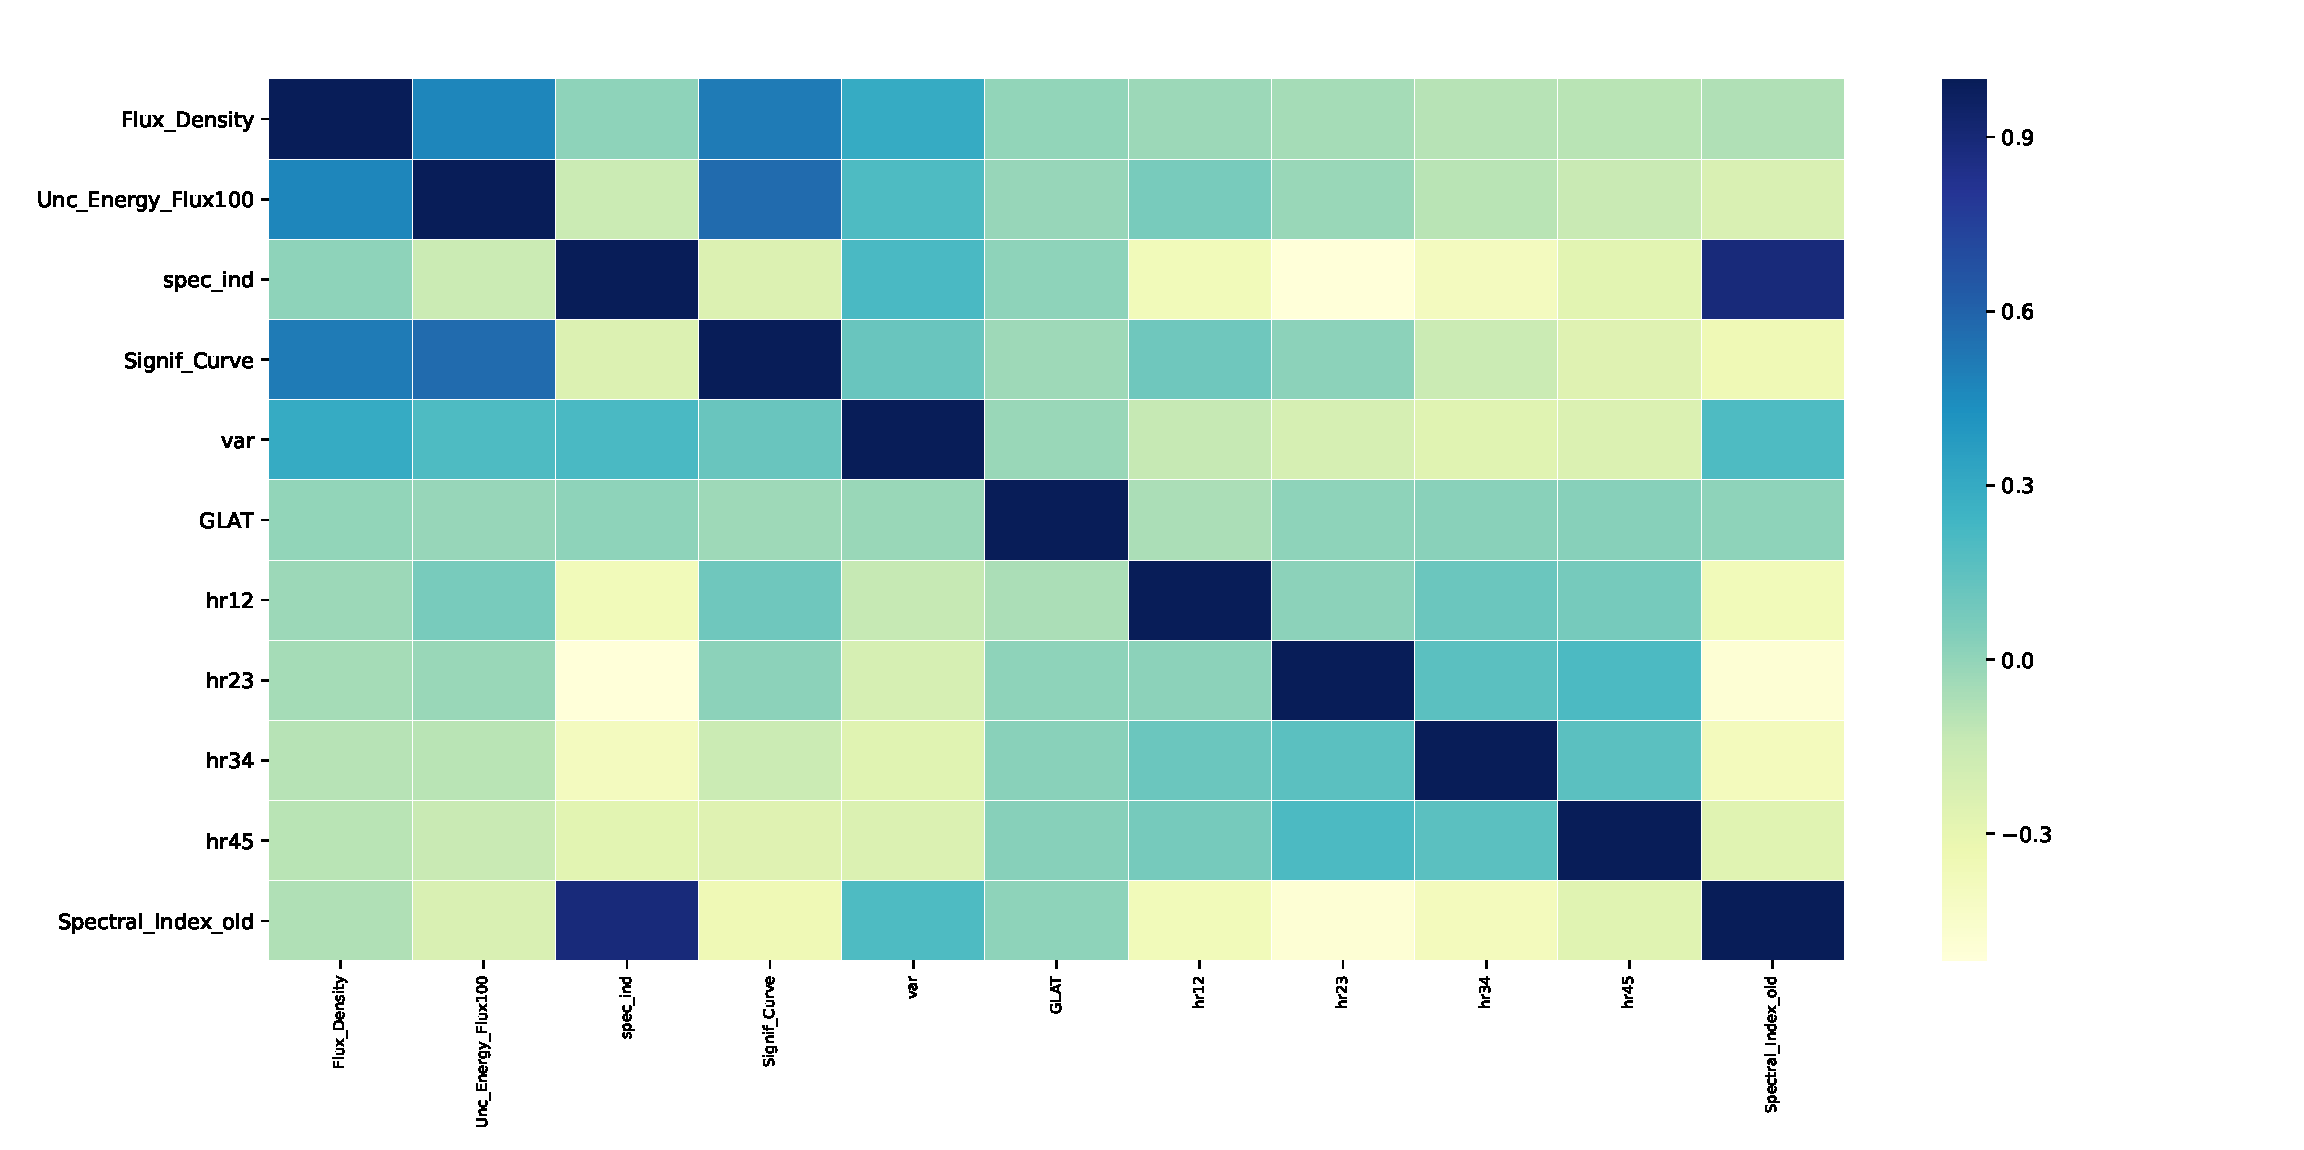
\includegraphics[width=\onepic\textwidth]{plots/correlation.pdf}
\caption{Correlation matrix for the most important features}
\label{fig:corr}
\end{figure}
[Add Table]\\

The features used for our analysis follow the same idea as the previous studies. The features, along with statistical and methodological details, are given below. A correlation matrix is presented for the most important features as well. The matrix is important for the case where there might be redundant features, in which case using only one of the two features would be a better idea.\\




Our initial hypothesis was that certain features would be more important for classification than others. For instance, as shown below, one can see a clear distinction between the regimes of AGNs and Pulsars, based on spectral idex and significant curvature. [Add image] While not clearly obvious from the get go, we were also interested in comparing the importance of features based on the algorithms that we were using. Due to the difference in the basic method of Random Forests and Neural Networks, we expected a slight shift in their reliance on certain features. Despite that we hypothesized that features with the most contribution would be among spectral index, variability, and the curvature; as already observed by Parkinson et. al. This is made clearer by the two figures below, which highlight the separation of PSR and AGN. The separation is seen to be much easier when spectral index and curvature are used, as opposed to the flux and uncertainty on the flux.\\

\begin{figure}[h]
%\centering
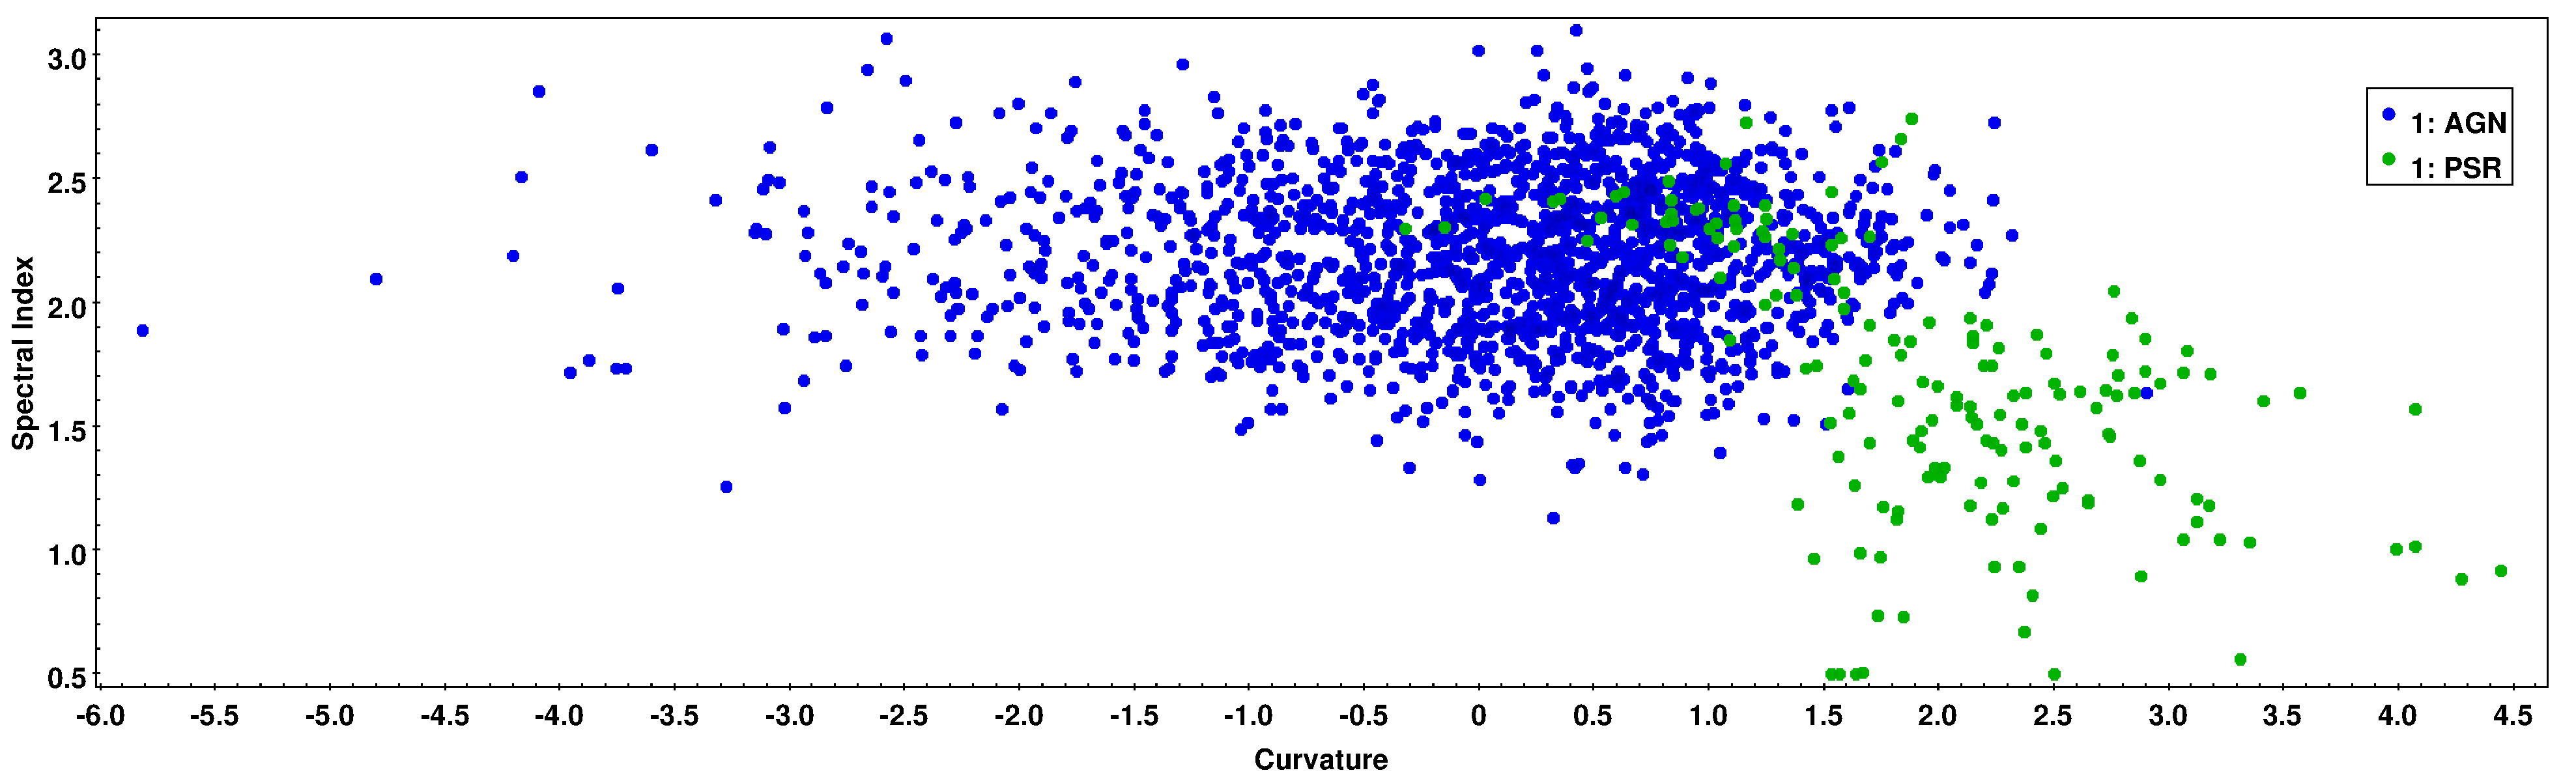
\includegraphics[width=\onepic\textwidth]{plots/signifcurvvsspecind2.pdf}
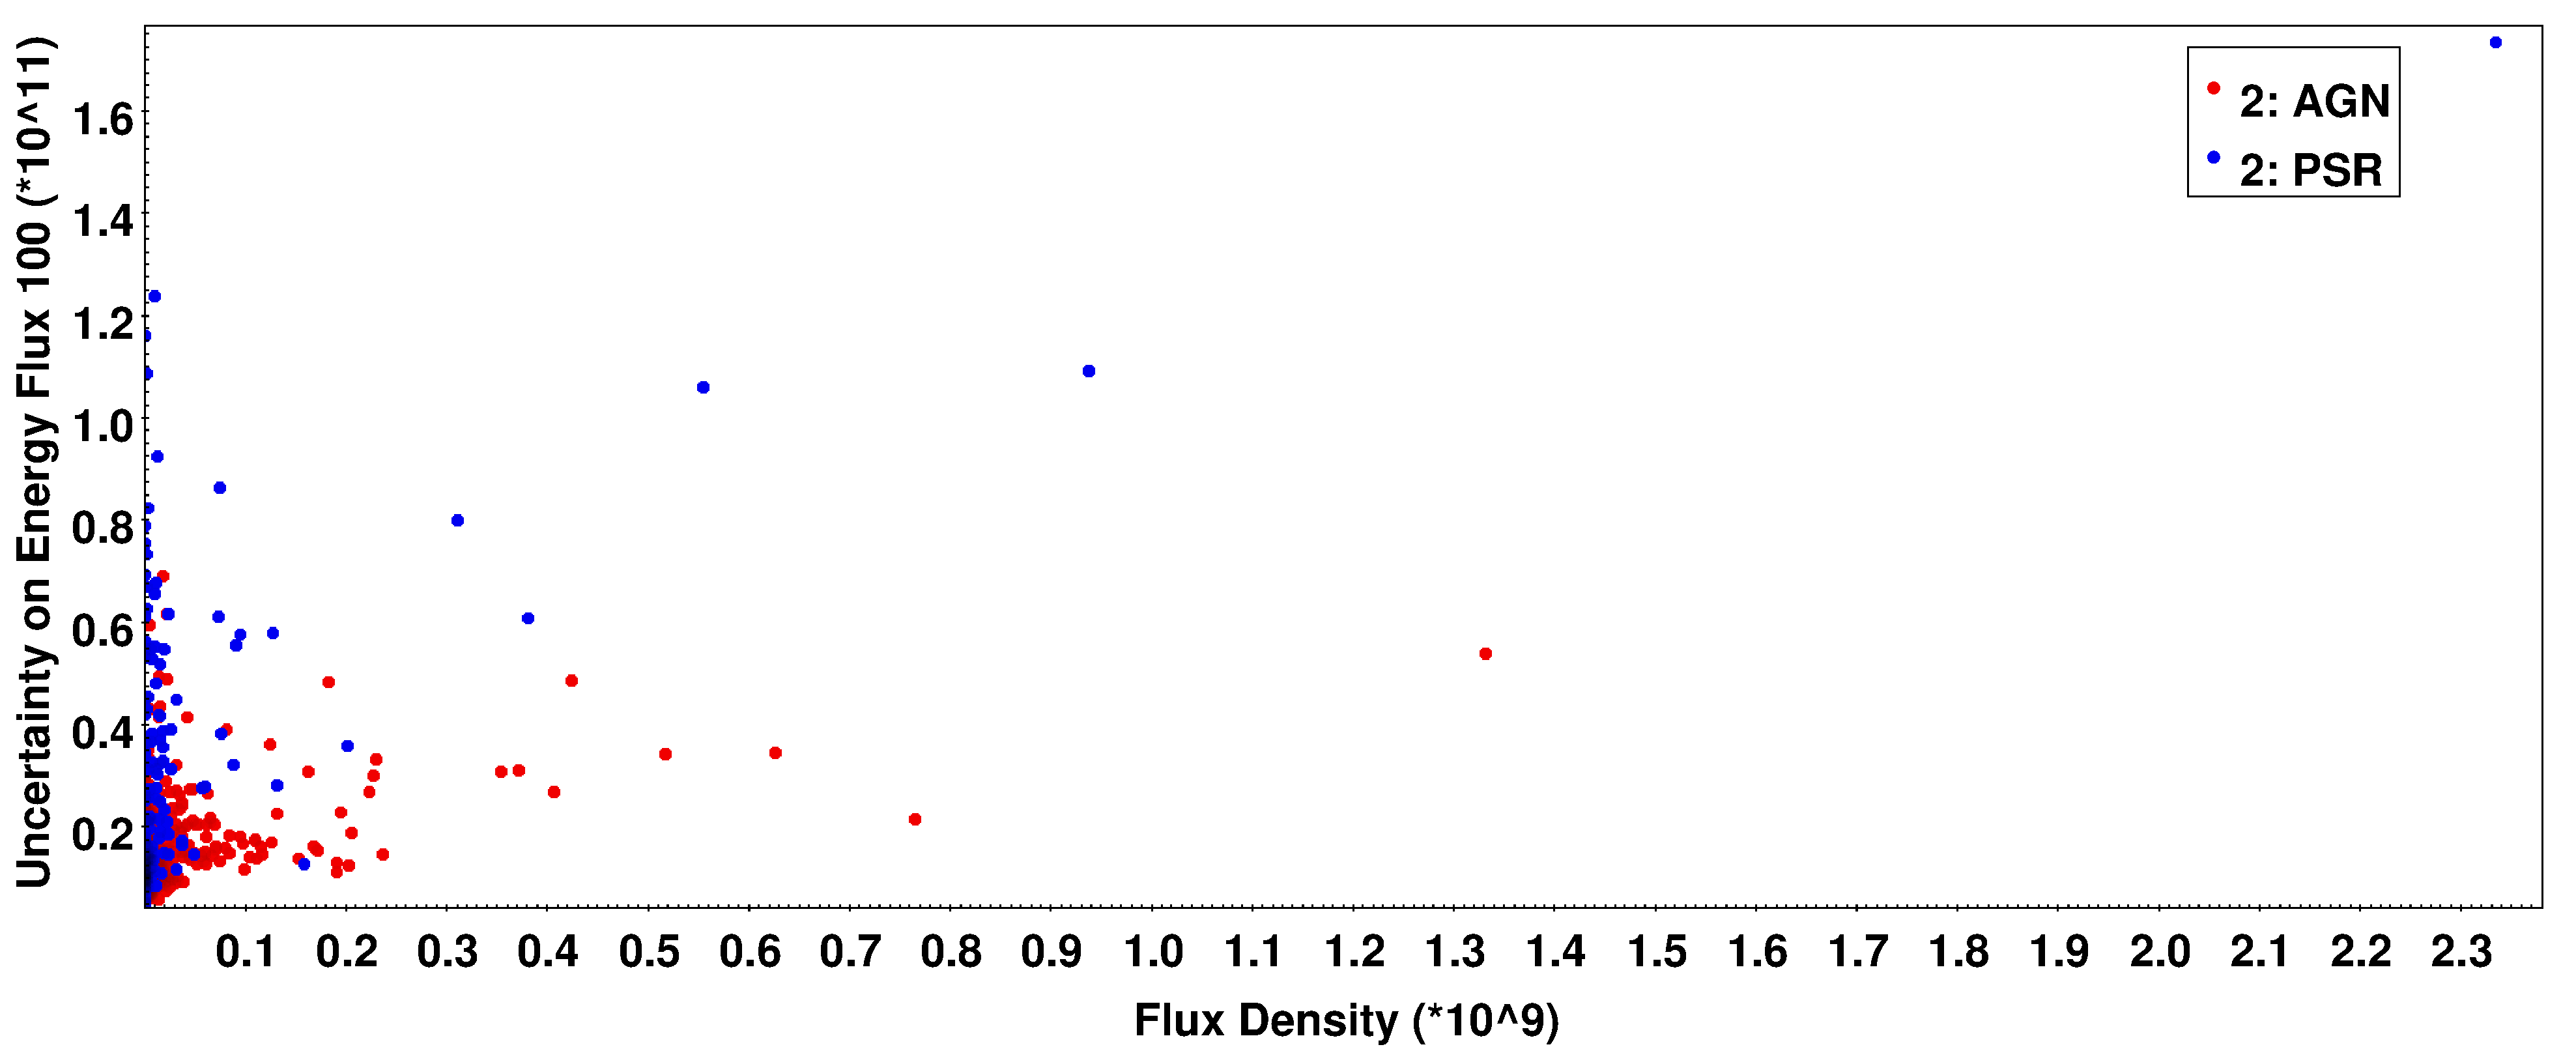
\includegraphics[width=\onepic\textwidth]{plots/fluxvsunc.pdf}
\caption{Separation of AGNs and PSRs from the 3FGL catalog based on different features}
\label{fig:corr}
\end{figure}




These importances were found to be consistent for various different algorithm parameters. So while the value might change a bit for different tree architechtures, for instance, the importances of these features were still pronounced. \\
\subsection{Comparison of the classification algorithms}

\end{comment}

\subsubsection{Random Forests}


\begin{figure}[h]
%\centering
\hspace*{-0.5cm}
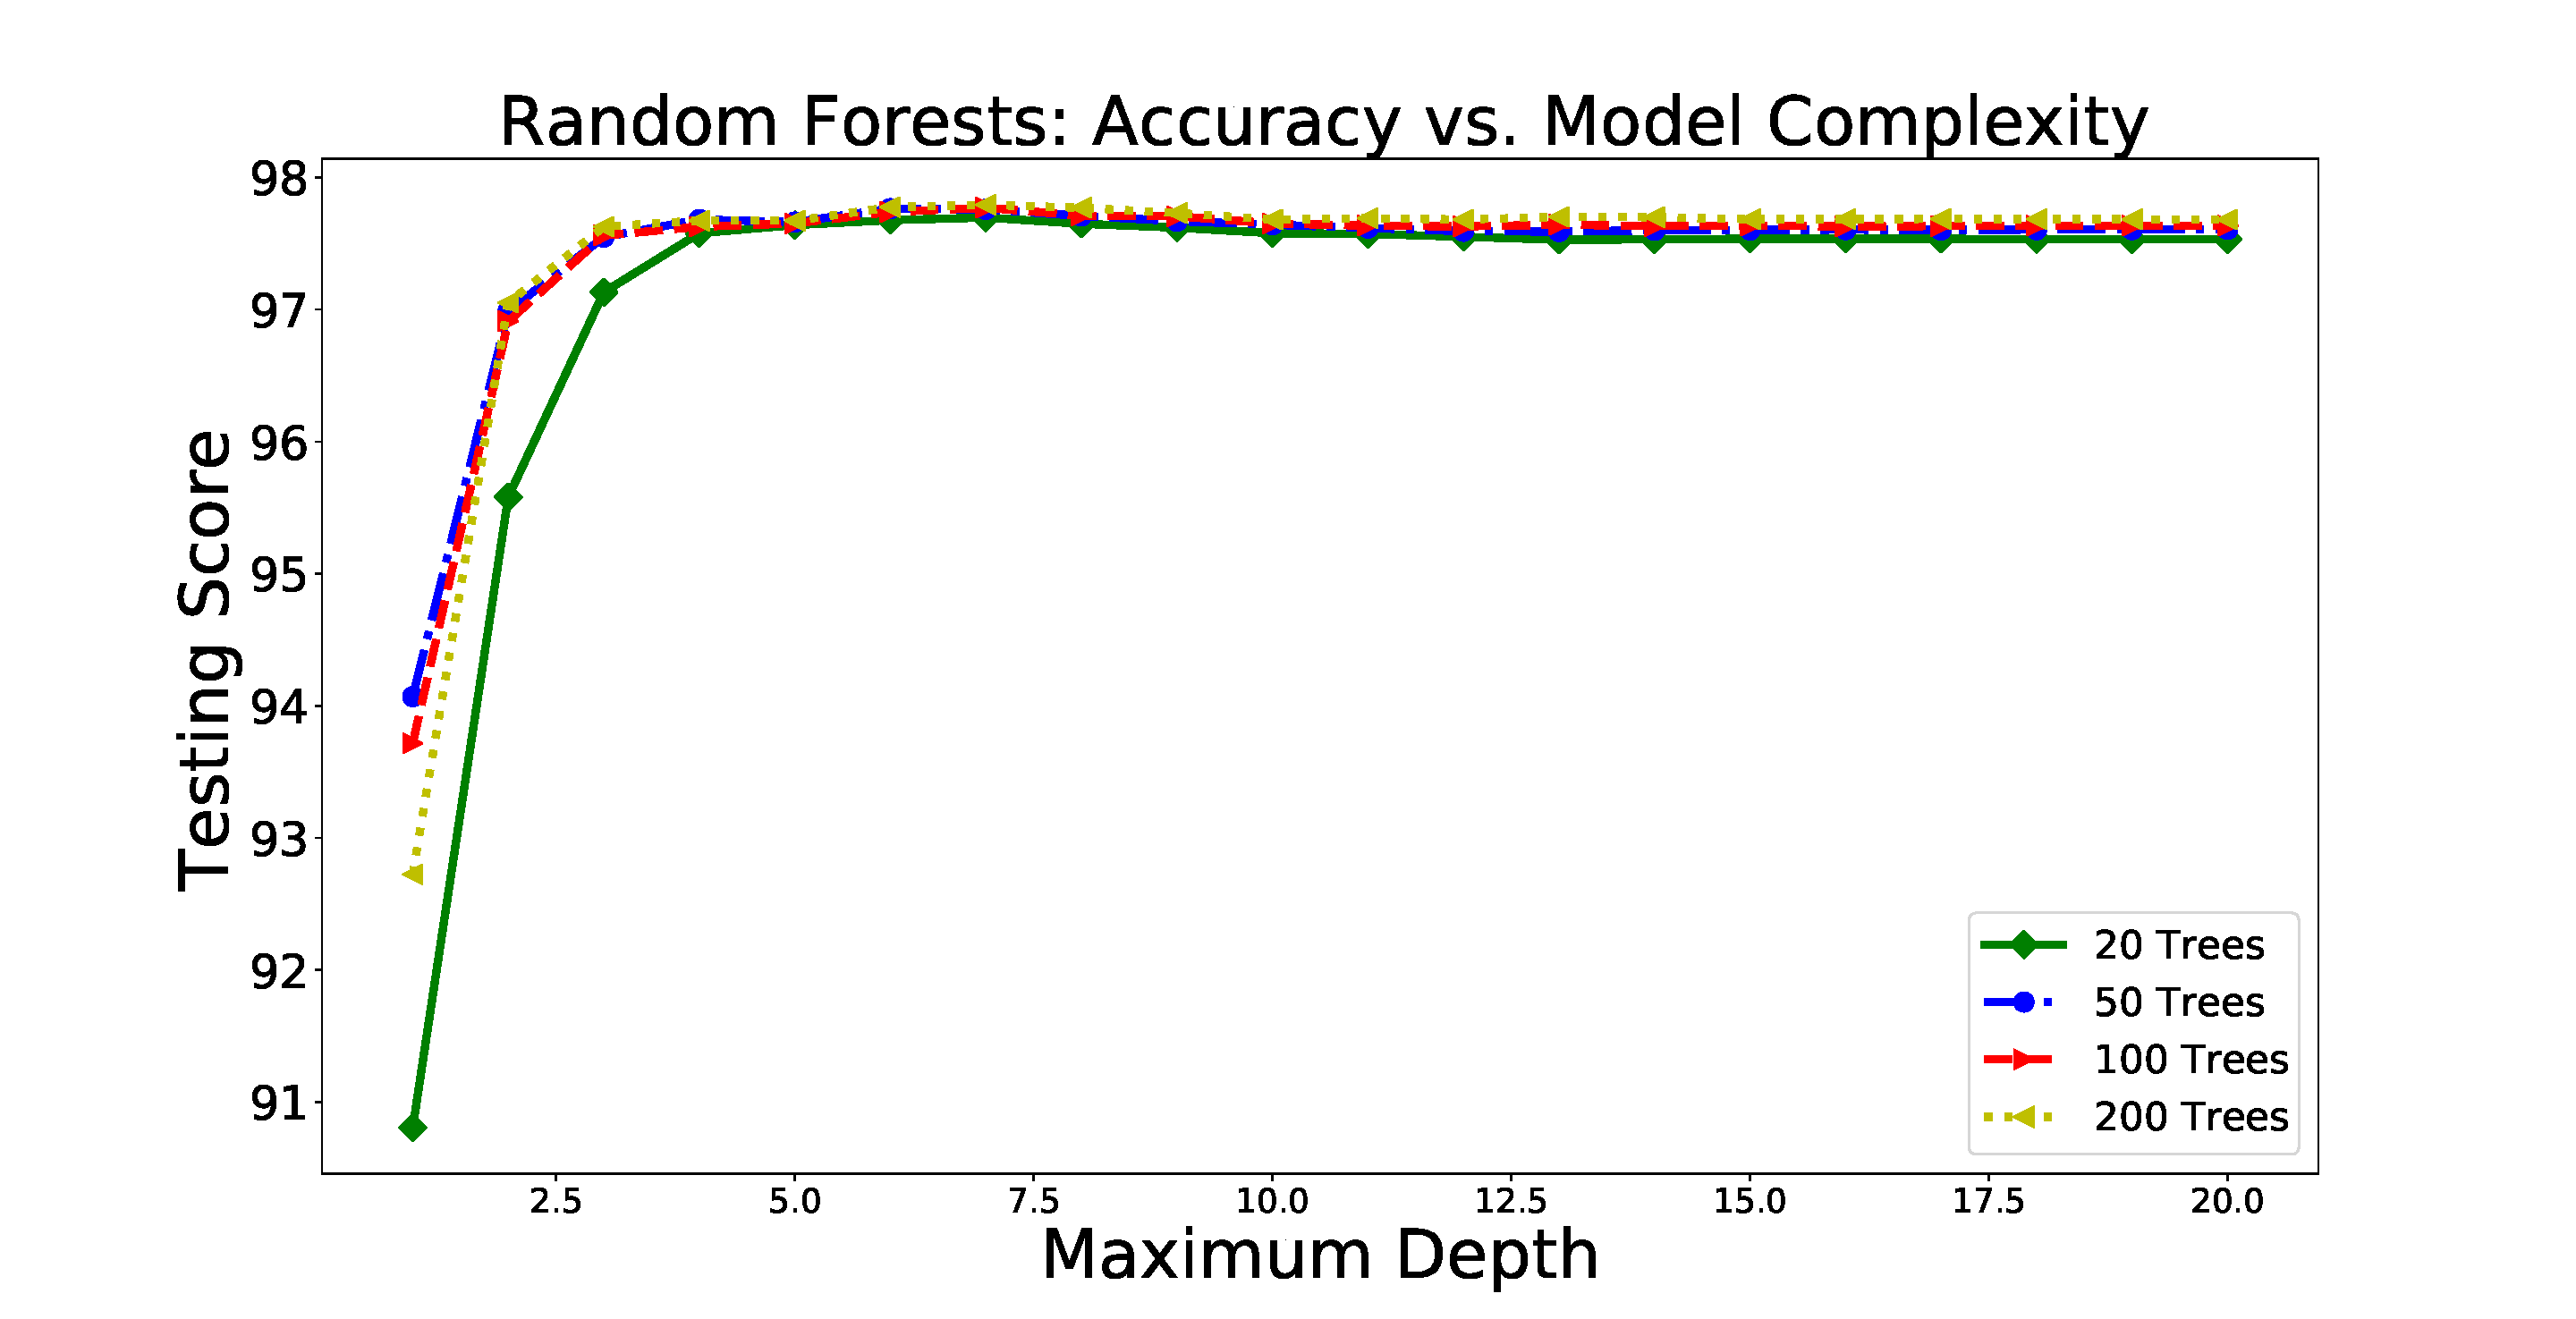
\includegraphics[width=0.5\textwidth]{plots/rf_train}
%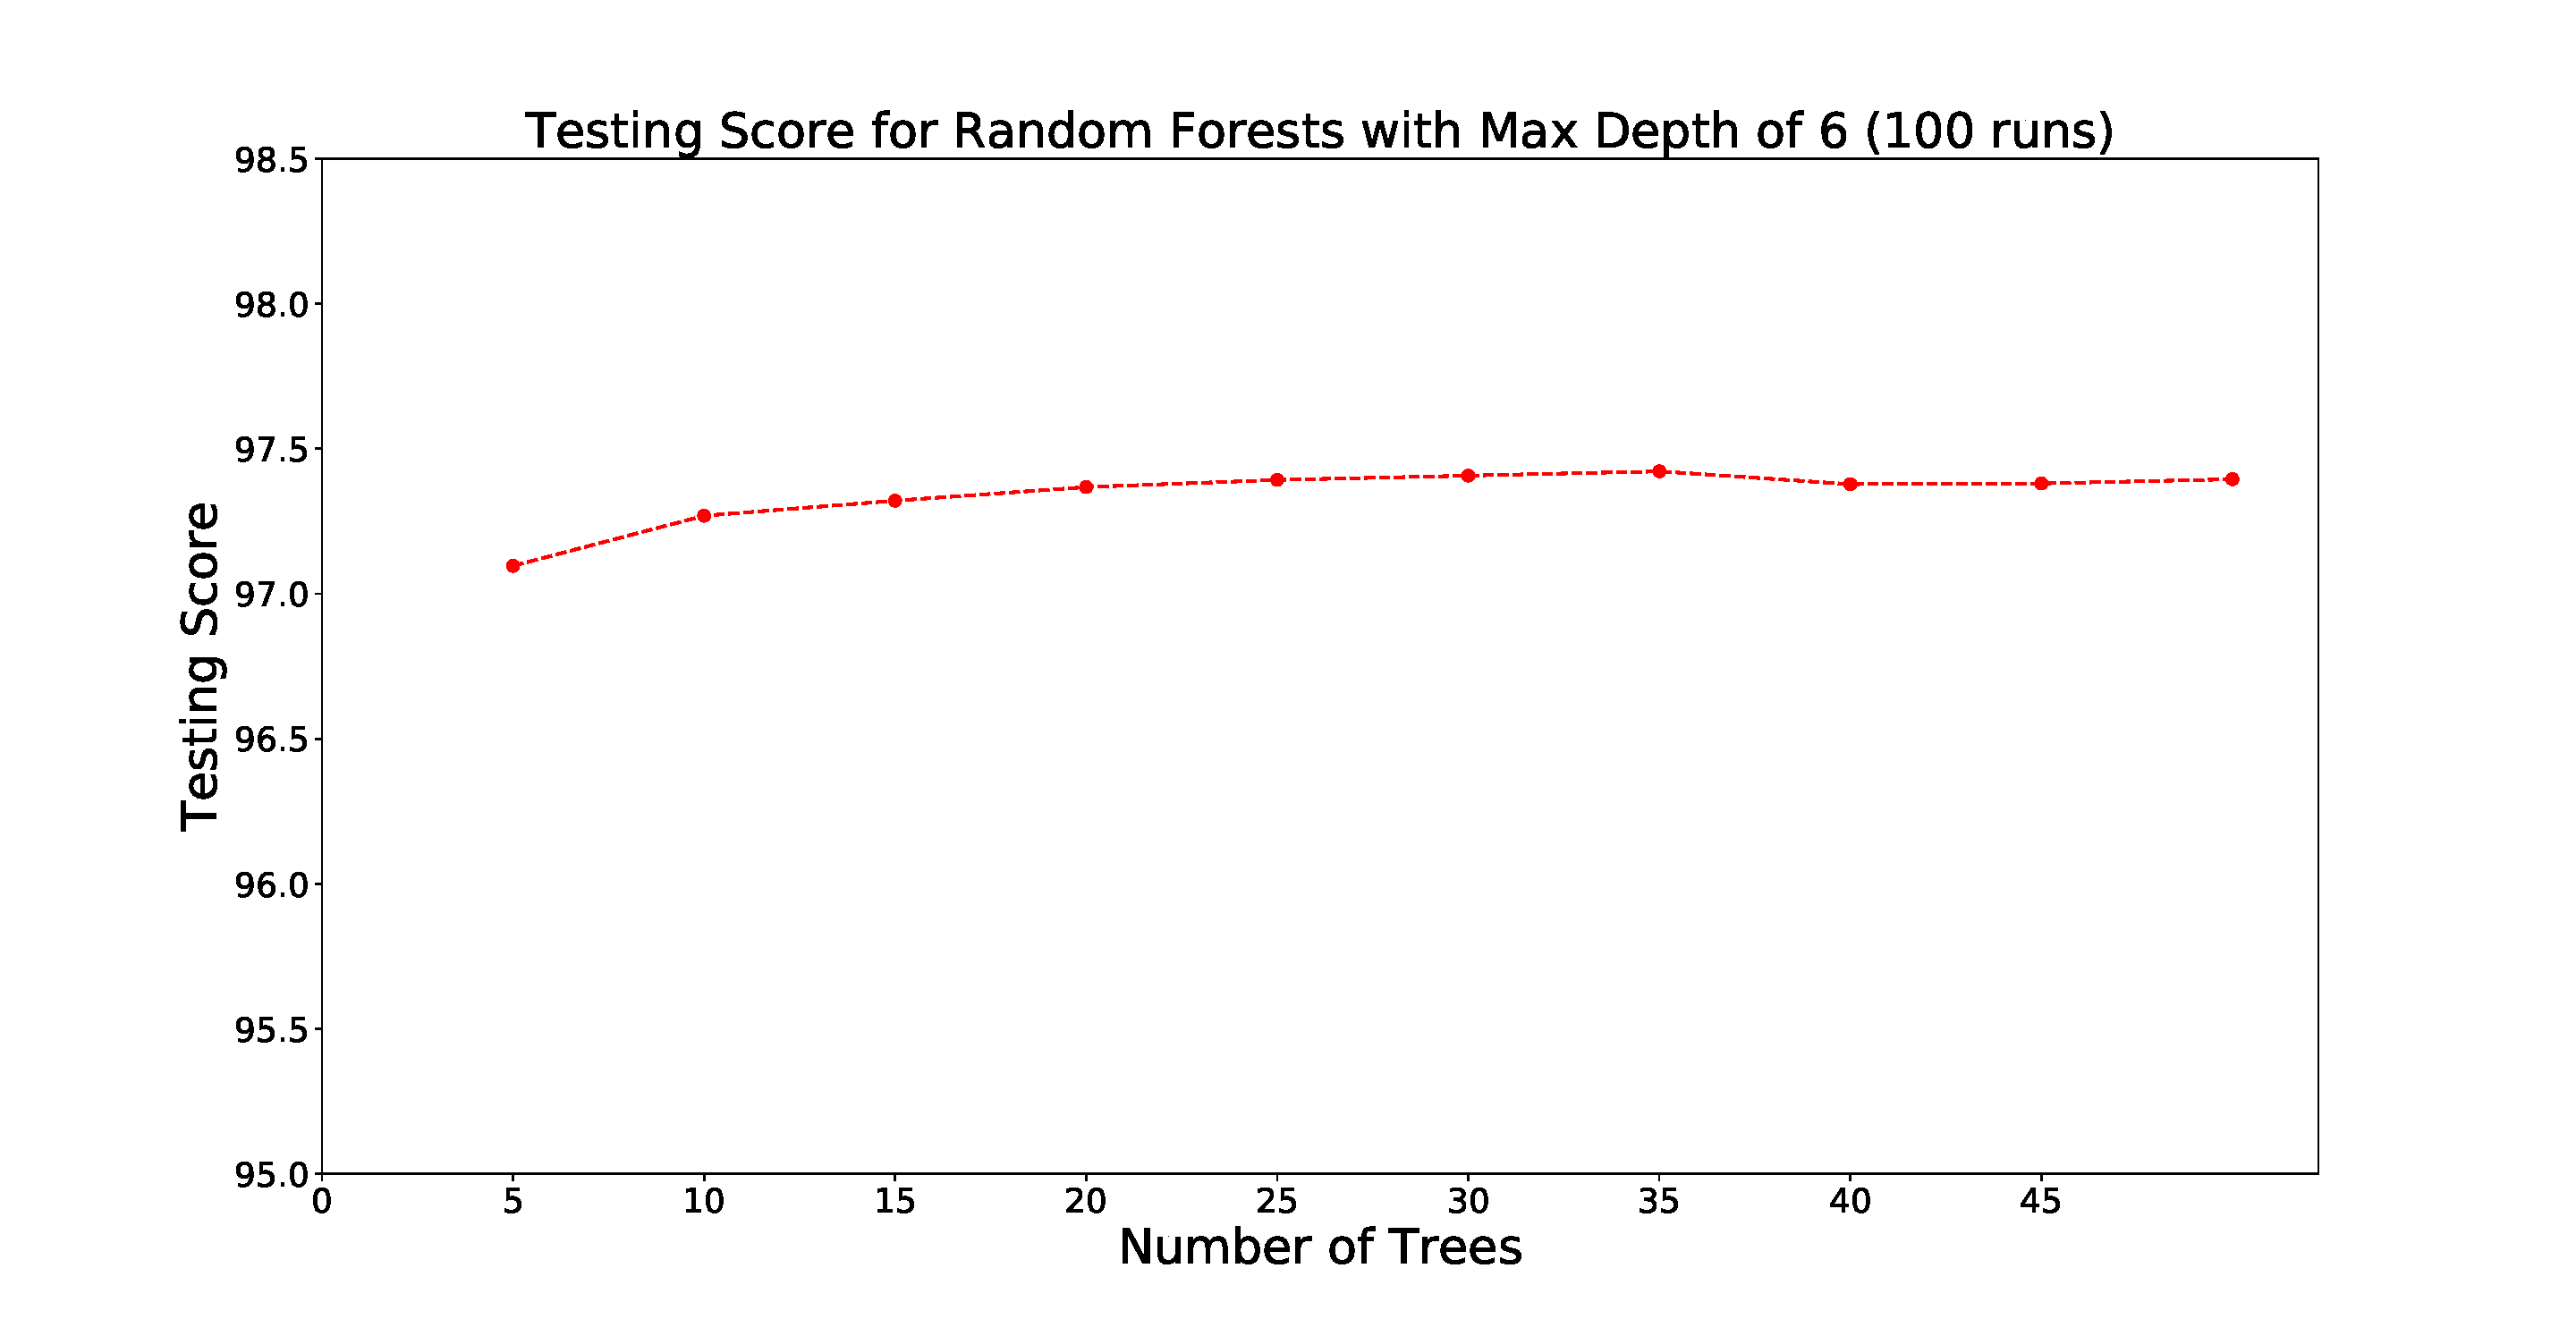
\includegraphics[width=\twopicsp\textwidth]{plots/6md_trees_weighted}
\caption{
Test score of RF classification as a function of the number of trees and maximal depth of trees.
%\dima{I think we should stop at 15 here since results don't change for max depth above 15.}
}
\label{fig:RF_complexity}
\end{figure}

The two main parameters characterizing the random forest algorithm are the number of trees and the maximum depth. 
Figure \ref{fig:RF_complexity} shows the dependence of the accuracy on the test sample as a function of maximum depth and the number of trees. For each line the number of trees is fixed.
The results for each point are averaged over 100 runs.
We have performed weighting the data by the inverse numbers of pulsars and AGNs to take into account that there are more AGNs than pulsars. Training on data without the inverse weighting did not have a significant effect on the accuracy.
We notice that the test score does not decrease with larger complexity of the model 
(larger number of free parameters due to larger maximal depth of trees).
This is due to the random choice of a subset of features at each node.
For the final algorithm, we will use a RF with 200 trees and a maximum depth of 8 trained on inversely weighted data. A depth greater than 8 results in a drop in performance. For the objective function we chose the gini index, which uses the square of the class probabililties for minimization.\\
%In the case of training, we found no significant differences when using weights for our data set. However, we chose to use a inversely weighted dataset since that allows us to generalize the algorithm more. The influence of weights will also be discussed more in the case of unassociated data, in the next section.
%After running tests on various architectures we chose a Random Forest with 20 trees to avoid over-fitting, and a maximum depth of 12.
%\dima{
%Why 12? It looks like 4 or 5 is already good enough.
%We should write here an equation for test score in case of weighted data.}

In tree-based algorithms, one can calculate feature importance by using the averaged reduction of impurity for nodes involving the different features. The feature importances for the case of two different RF algorithms: 20 trees with max depth 12 and 50 trees with max depth of 6 are shown in Table \ref{tab:feat_imp}.
We find that the four most important features are spectral curvature, hardness ratio of the last two energy bins, spectral index, and variability, which follow the trend regardless of hyper-parameters chosen.
%Since Random forests are based on decision trees, they allow us to characterize feature importances based on how helpful a feature was to split a tree. In our case, using all 10 features discussed above we found the following feature importances for two architectures of random forests with similar accuracies of 97.5:\\


\begin{table}[!h]
    \tiny
    \centering
    \renewcommand{\tabcolsep}{1mm}
\renewcommand{\arraystretch}{1}

    \begin{tabular}{|c|c|c|}
    \hline
    Feature &  20 trees, depth 2& 50 trees, depth 6\\
    \hline
    Flux Density& 0.04 & 0.05        \\
    \hline
    Unc Energy Flux100& 0.07     & 0.08 \\
    \hline %\midrule   -> aakash do you mean this?
   Spectral Index & 0.13     &   0.11\\
    \hline %\midrule   -> aakash do you mean this?
    Significant curvature& 0.33 &0.29  \\
    \hline
   var&  0.06   &  0.10  \\
    \hline %\midrule   -> aakash do you mean this?
    hr12& 0.03 &0.03 \\
    \hline
     hr23& 0.03 &0.04 \\
    \hline
    hr34& 0.02 &0.03 \\
    \hline
   hr45& 0.25 &0.21 \\
    \hline
    GLAT&0.01&0.02\\
    \hline
    \end{tabular}
    \vspace{0.4cm}
    \caption{Feature importances for two RF algorithms.}
    \label{tab:feat_imp}
\end{table}

%Our hypothesis about feature importances turned out to be correct, as curvature, variability, and spectral index were the most important features. The last hardness ratio was also seen to be quite important, most probably reflecting the end of the spectrum where the AGNs and PSRs shift from each other.\\

In order to illustrate the separation of the PS into AGNs and pulsars, we retrain the RF algorithm using only two features: curvature significance and spectral index, and plot the resulting probabilities of classes in Figure \ref{fig:RF_domains}. These classification domains provide us with a look at the complexity of the network. As we can see the depth 4 outperforms depth 2. We decide to go higher on the depth and trees, since this plot is a 2-d estimation of a 10 feature problem, as we have only plotted for two of the main features. As can be seen in the figure, the colourer is redder closer to cluster of AGNs and bluer in areas with higher PSRs. The probabilities are shown for only one run, as a way of illustrating how the algorithm seperates different regions of the data-set. The higher the depth the more the probabilities becomes denser and the dense areas become smaller. For instance, one can see region of near zero probabilities in the depth of 4, as opposed to a depth of 2.  
\dima{Add discussion of the domains, e.g., overfitting, and selection of the final model for classification.}

\begin{figure}[h]
\hspace*{-1.5cm}
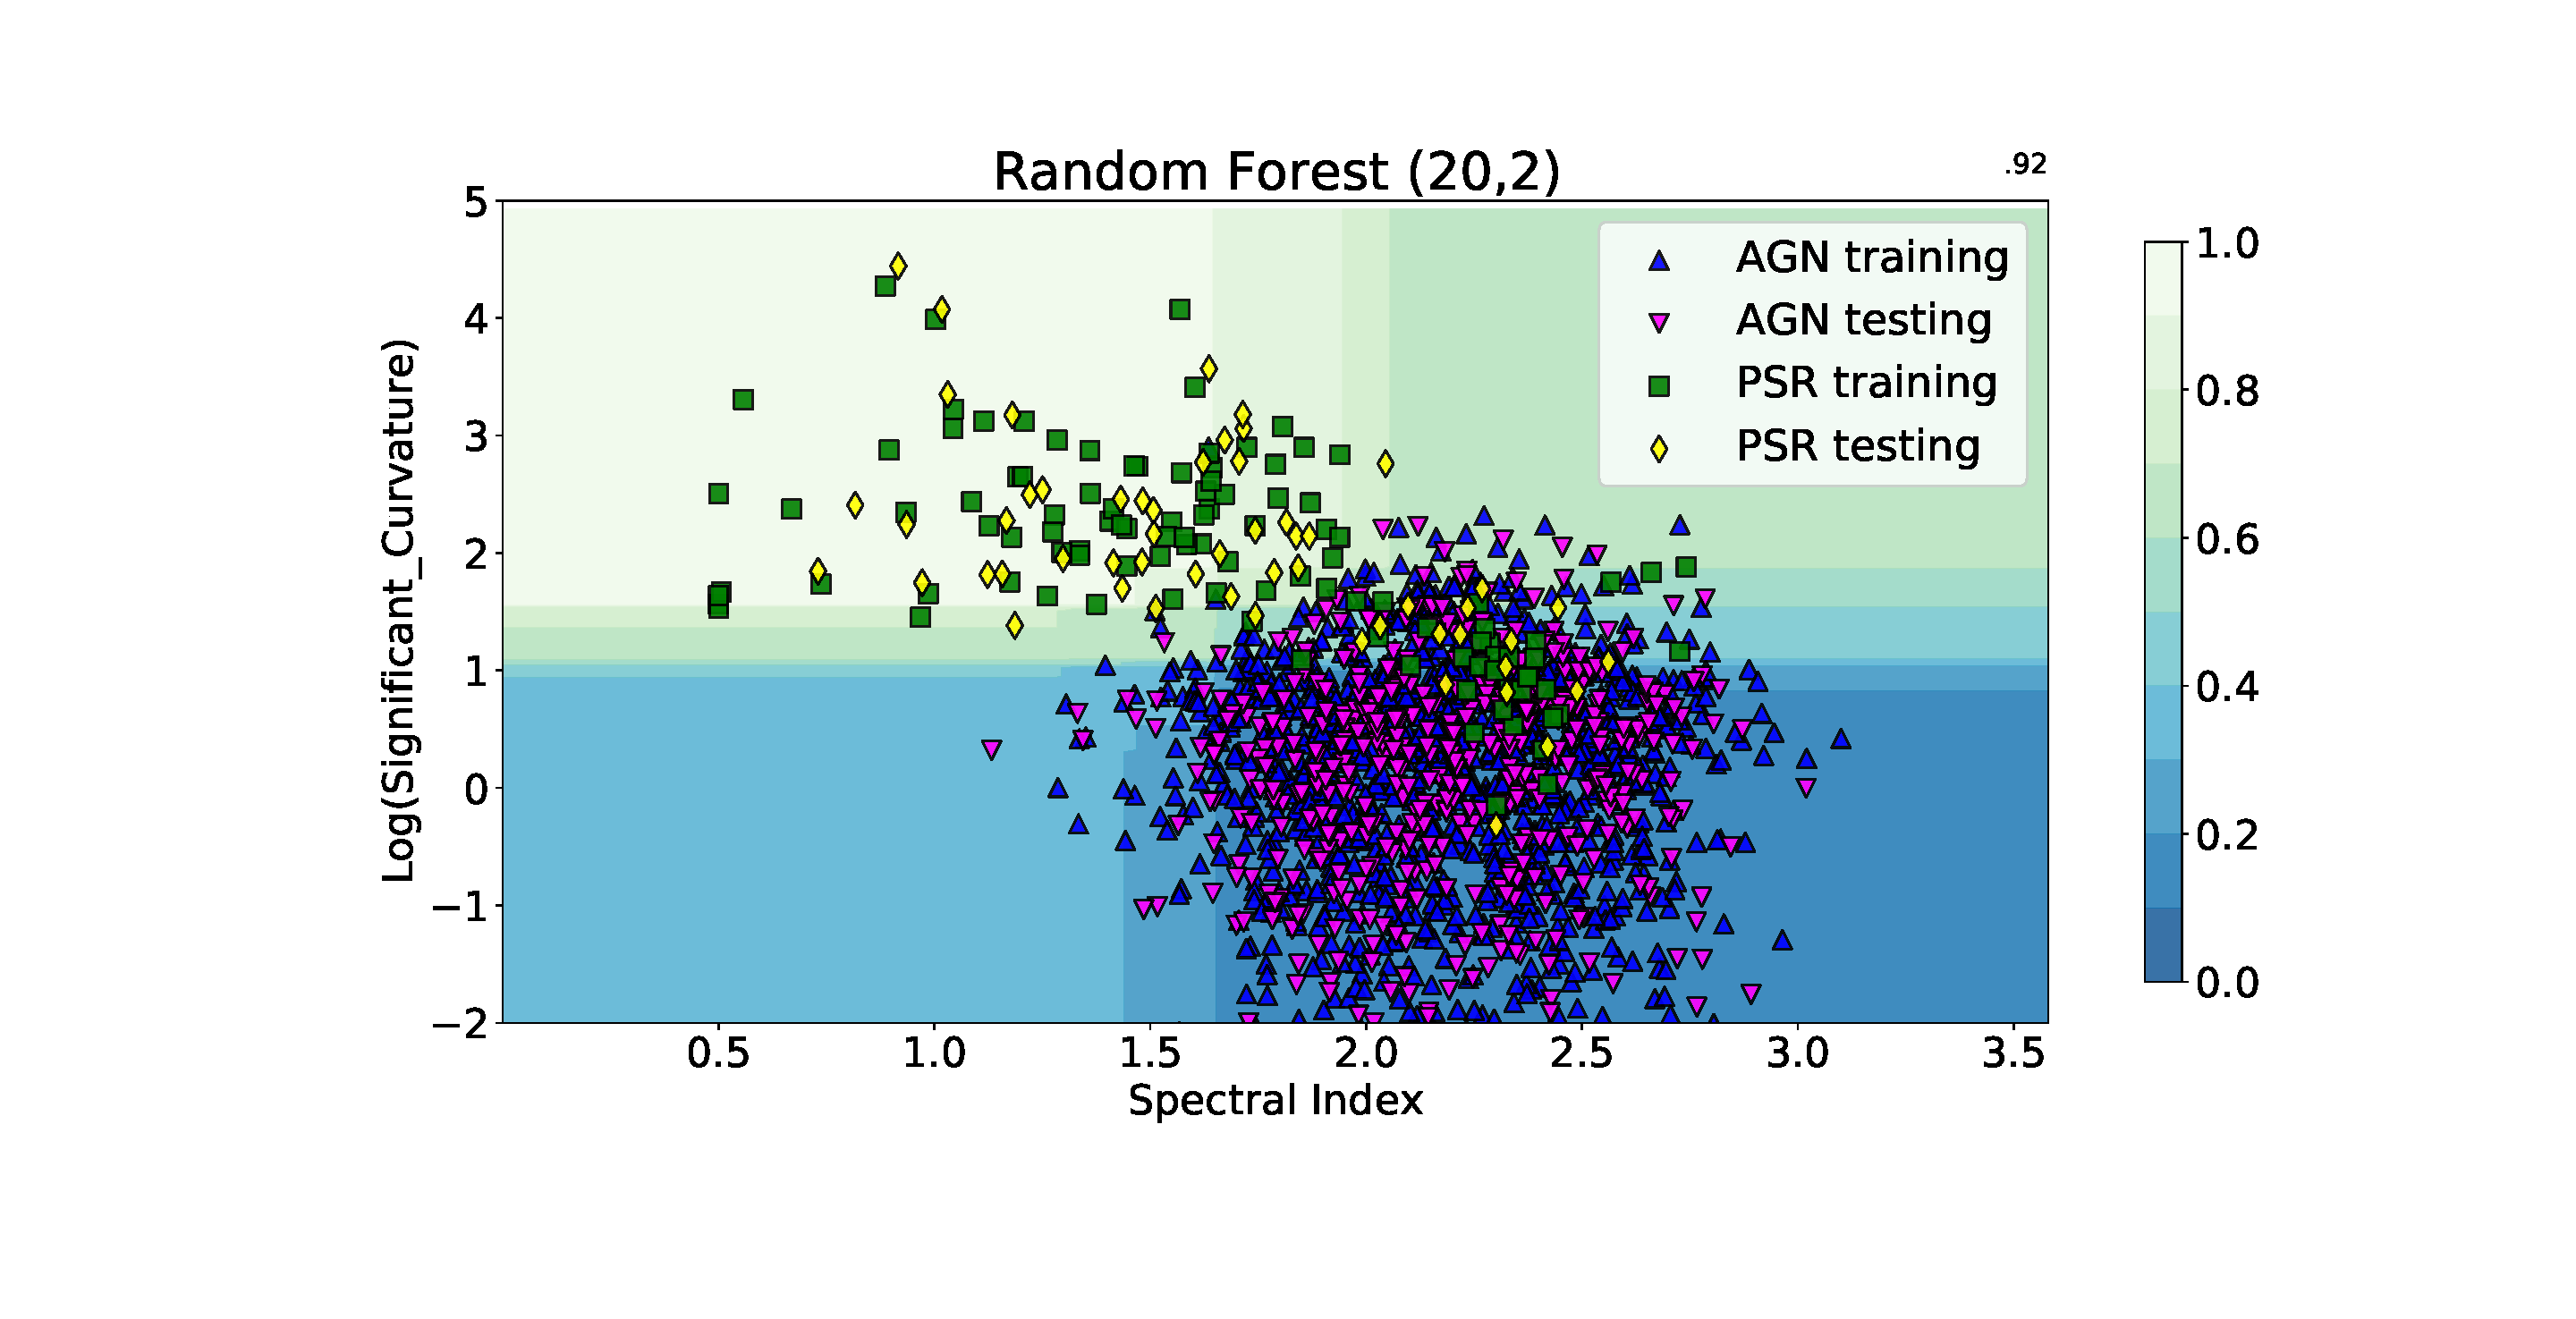
\includegraphics[width=0.6\textwidth]{plots/classification_domains/rf_20_2_final.pdf}
\hspace*{-1.5cm}
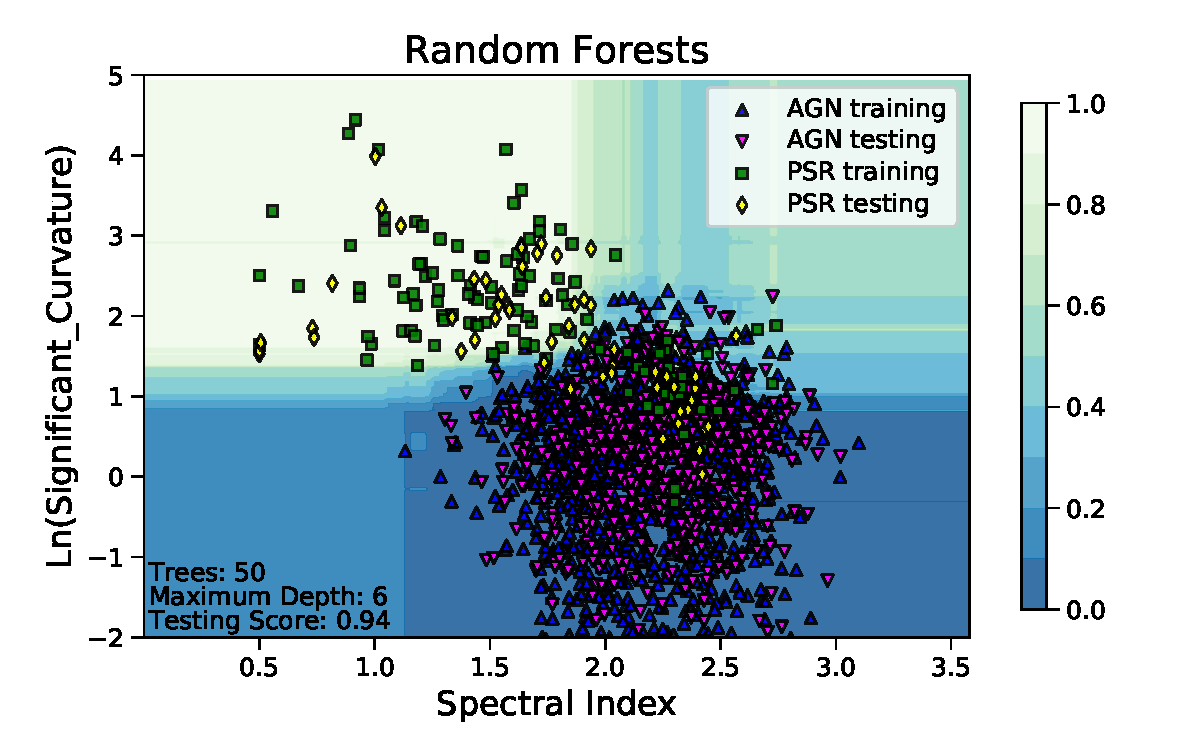
\includegraphics[width=0.6\textwidth]{plots/classification_domains/rf_50_6_final.pdf}
\caption{Classification Domains of RF: Differences in decision function for lower model complexity, compared to the chosen model.}  
\label{fig:RF_domains}
\end{figure}

%=======
%\begin{figure*}[h]
%\centering
%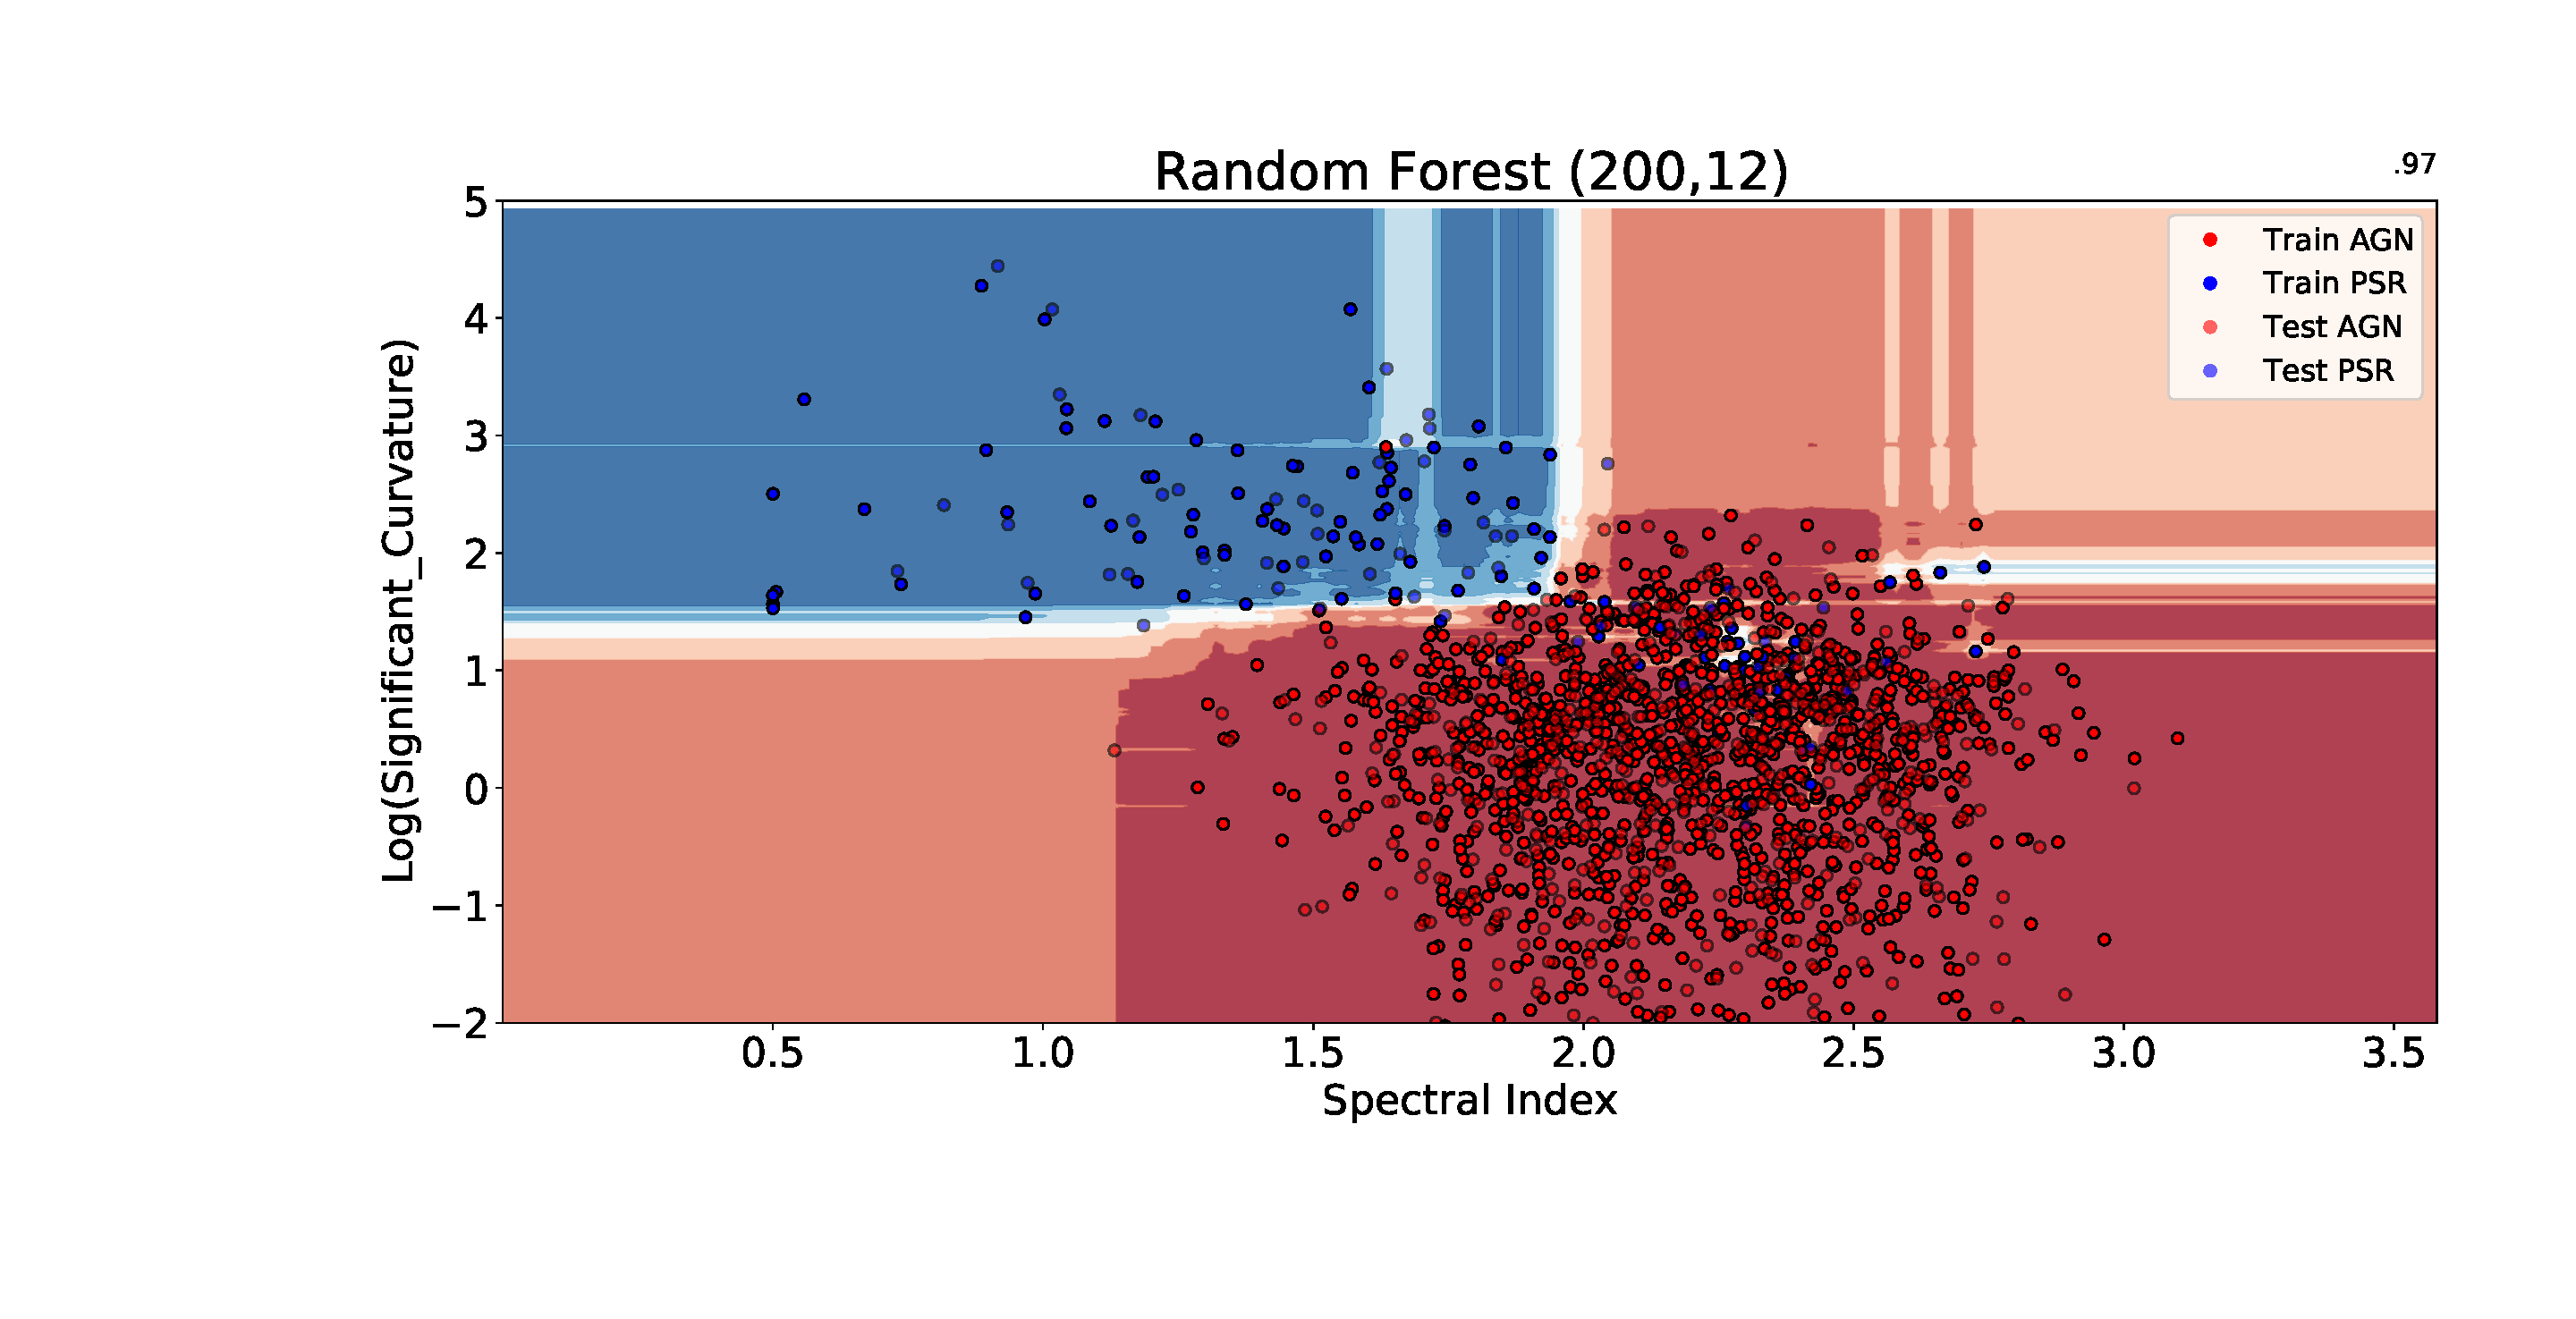
\includegraphics[width=\twocolumnwidth\textwidth]{plots/classification_domains/rf_200_12.pdf}\\
%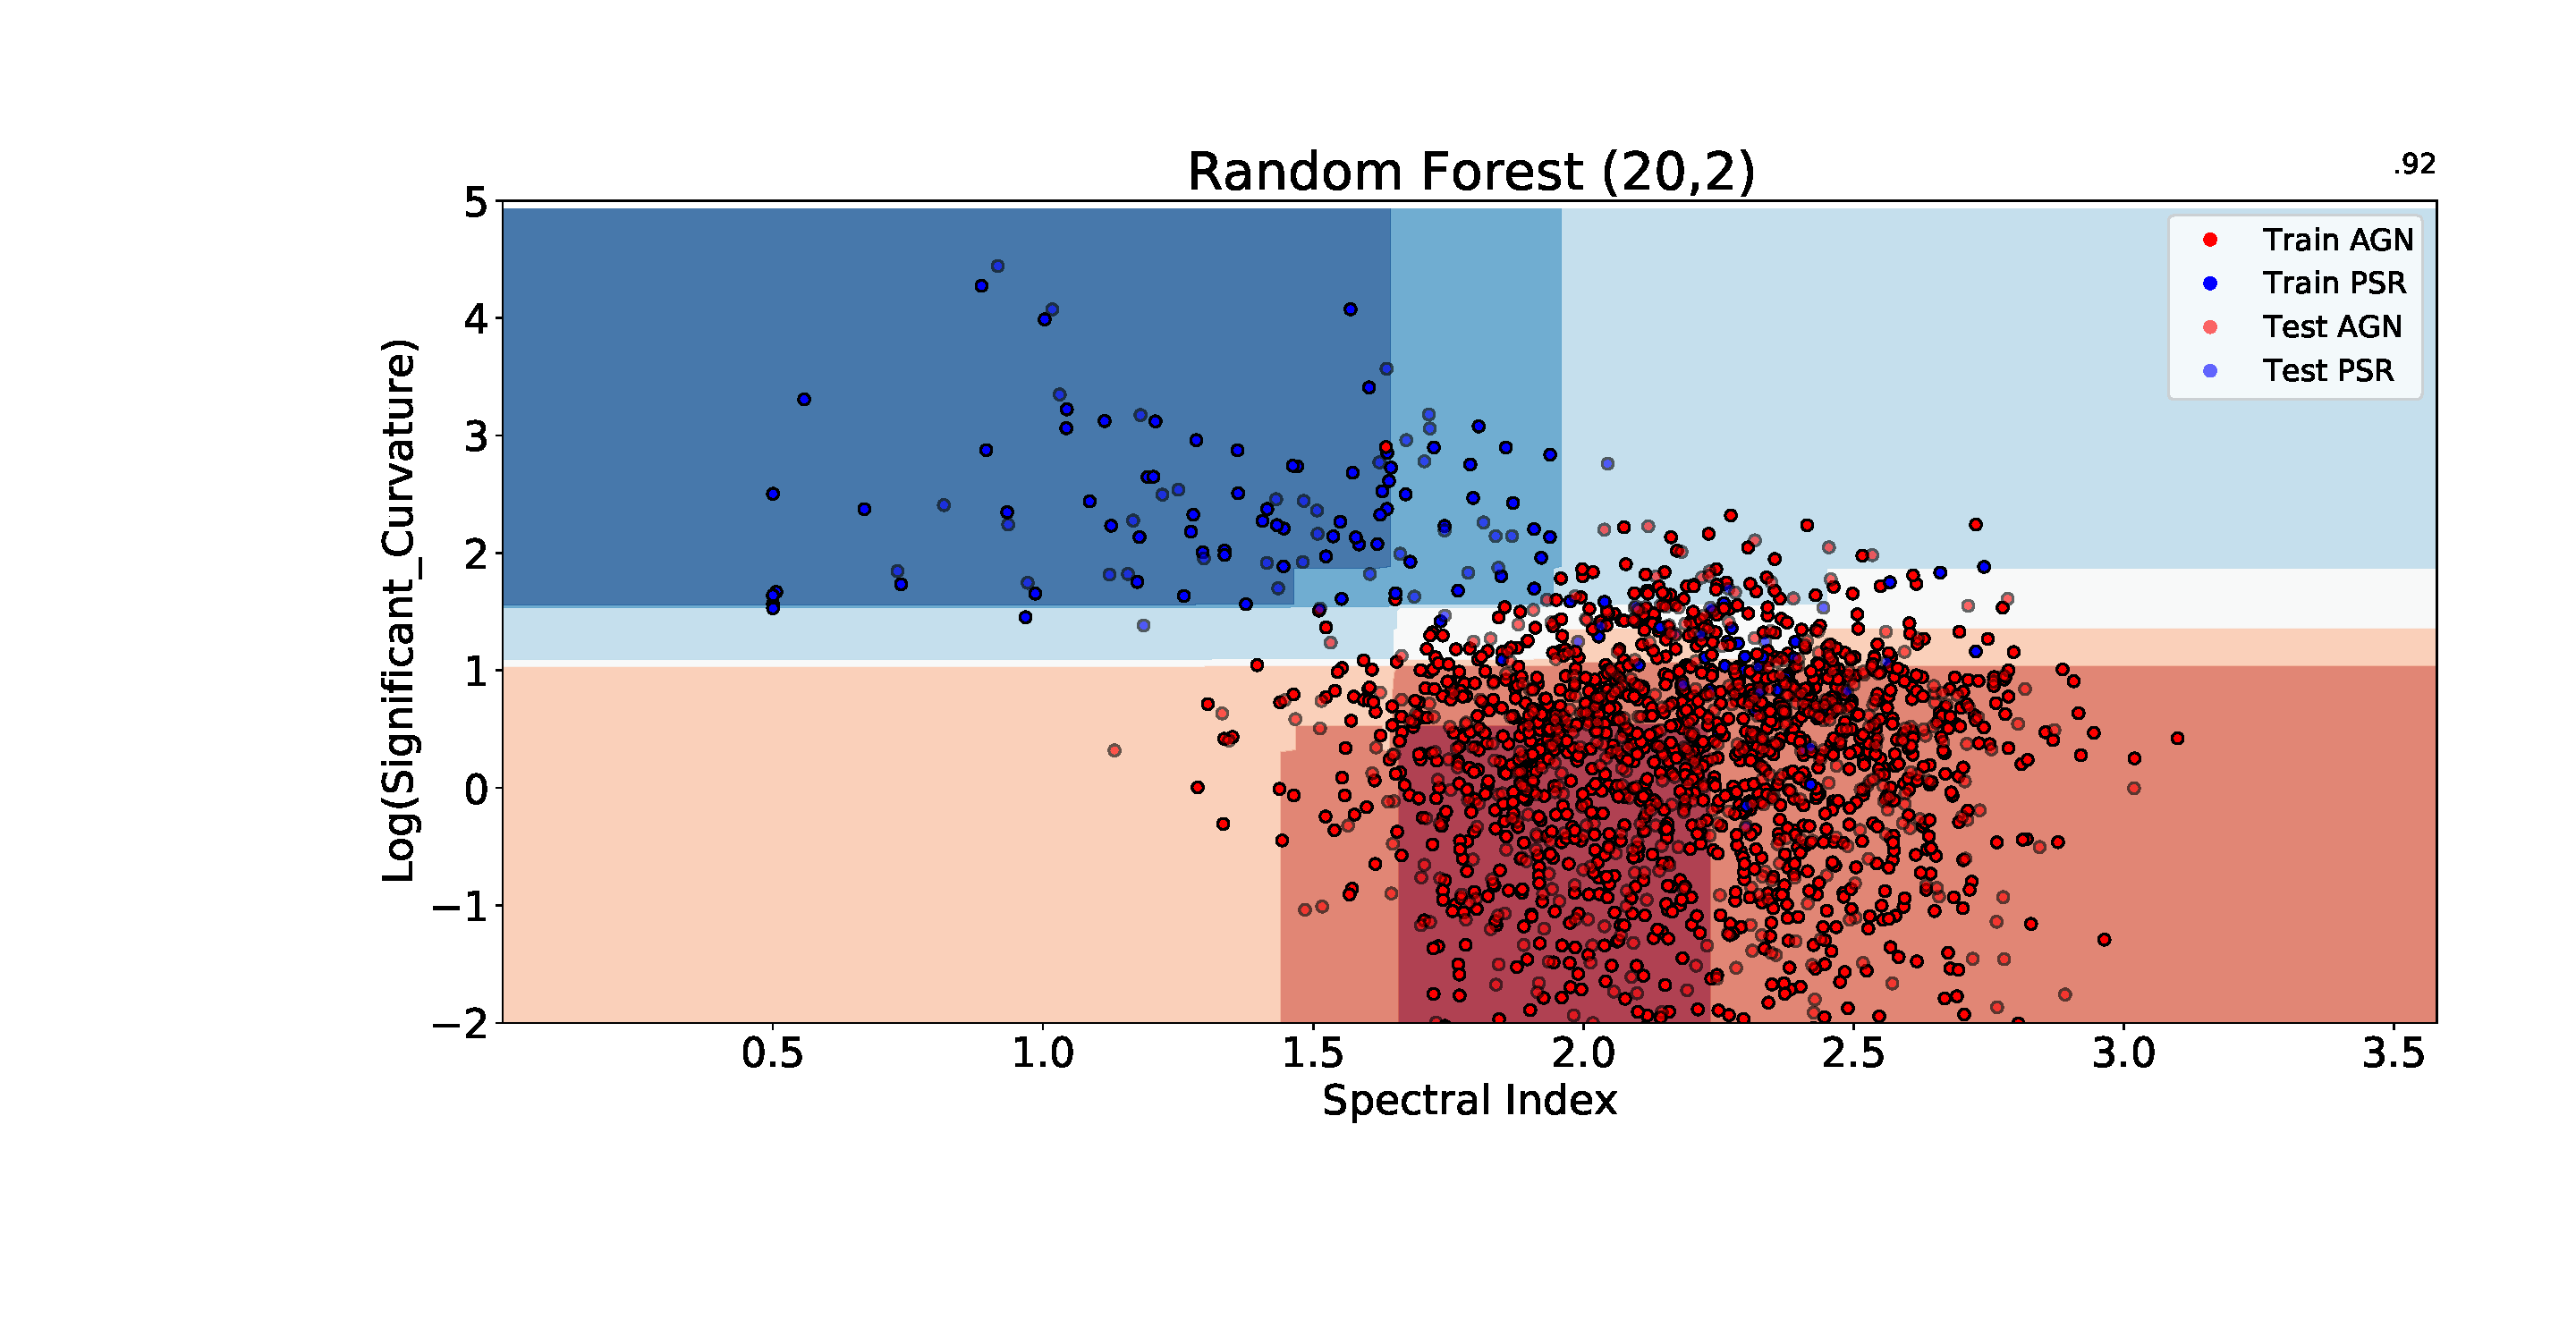
\includegraphics[width=\twocolumnwidth\textwidth]{plots/classification_domains/rf_20_2.pdf}
%>>>>>>> a522eecb66fa0cf6f440bc2907db2c42d74cac67
%\caption{Classification Domains of RF.  \dima{Why don't we show the domains for the final model, which we use for predictions?
%Moreover, it looks like for max depth 12 the model overfits the data, i.e., using max depth of 4 or 5 would be better for the final model.
%We should also add color bars for all domain plots and make the labels larger.}}
%\label{fig:RF_domains}
%\end{figure*}


\subsubsection{Neural Networks}

In the case of NN, the number of free parameters depends on the number of hidden layers and on the numbers of nodes.
Adding more than one hidden layer did not improve the accuracy of the classification.
In the following we will use NNs with only one hidden layer.
Dependence of the accuracy for test sample on the number of neurons in the hidden layer is shown in Figure \ref{fig:NN_neurons}.
Dependence on the number of epochs (number of iterations in fitting) is presented in Figure \ref{fig:NN_epochs}. 
The methods used to solve the loss function are L-BFGS and ADAM. L-BFGS (Limited memory Broyden-Fletcher-Goldfarb-Shanno) is an approximation of the quasi-newtonian BFGS method. The BFGS method uses the full inverse of the nxn Hessian matrix to find the direction of movement for minimizing the gradient. The limited memory counterpart however, only stores a smaller representation of the full matrix. This makes this method much faster for larger data-sets.\\
ADAM on the other hand belongs to a realtively newer family of algorithms which use gradient descent. Gradient descent is a first-order method to find the local minima or maxima of a differentiable function. Nowadays, this process is made more efficient by taking the gradient from parts of the data-set instead of the entire data-set itself. This is called stocahstic gradient descent, since the data is selected randomly. ADAM is a newer approach of the stochastic family using adaptive network learning rates for every parameter. ADAM is usually preferred for Neural Networks with big data-sets.\\ 
%\dima{Discuss L-BFGS and ADAM methods here. I don't understand where you can use tanh and relu activations, if we have only one hidden layer with classification for output.}

\begin{comment}
 we were concerned with the number of epochs that one would need to tweak, along with a dependence on the number of neurons in the hidden layers. A final improvement involved checking whether multiple hidden layers would actually add to such a classification algorithm or not.\\
As can be seen in the figure, with the specific stochastic gradient method ADAM, the number of epochs required are higher since ADAM converges slow. However, after around 200 epochs the accuracy saturates and reached the same as the lbfgs solver, which converges faster for smaller data-sets. \\
\end{comment}

\begin{figure}[h]
%\centering
\hspace*{-0.5cm}
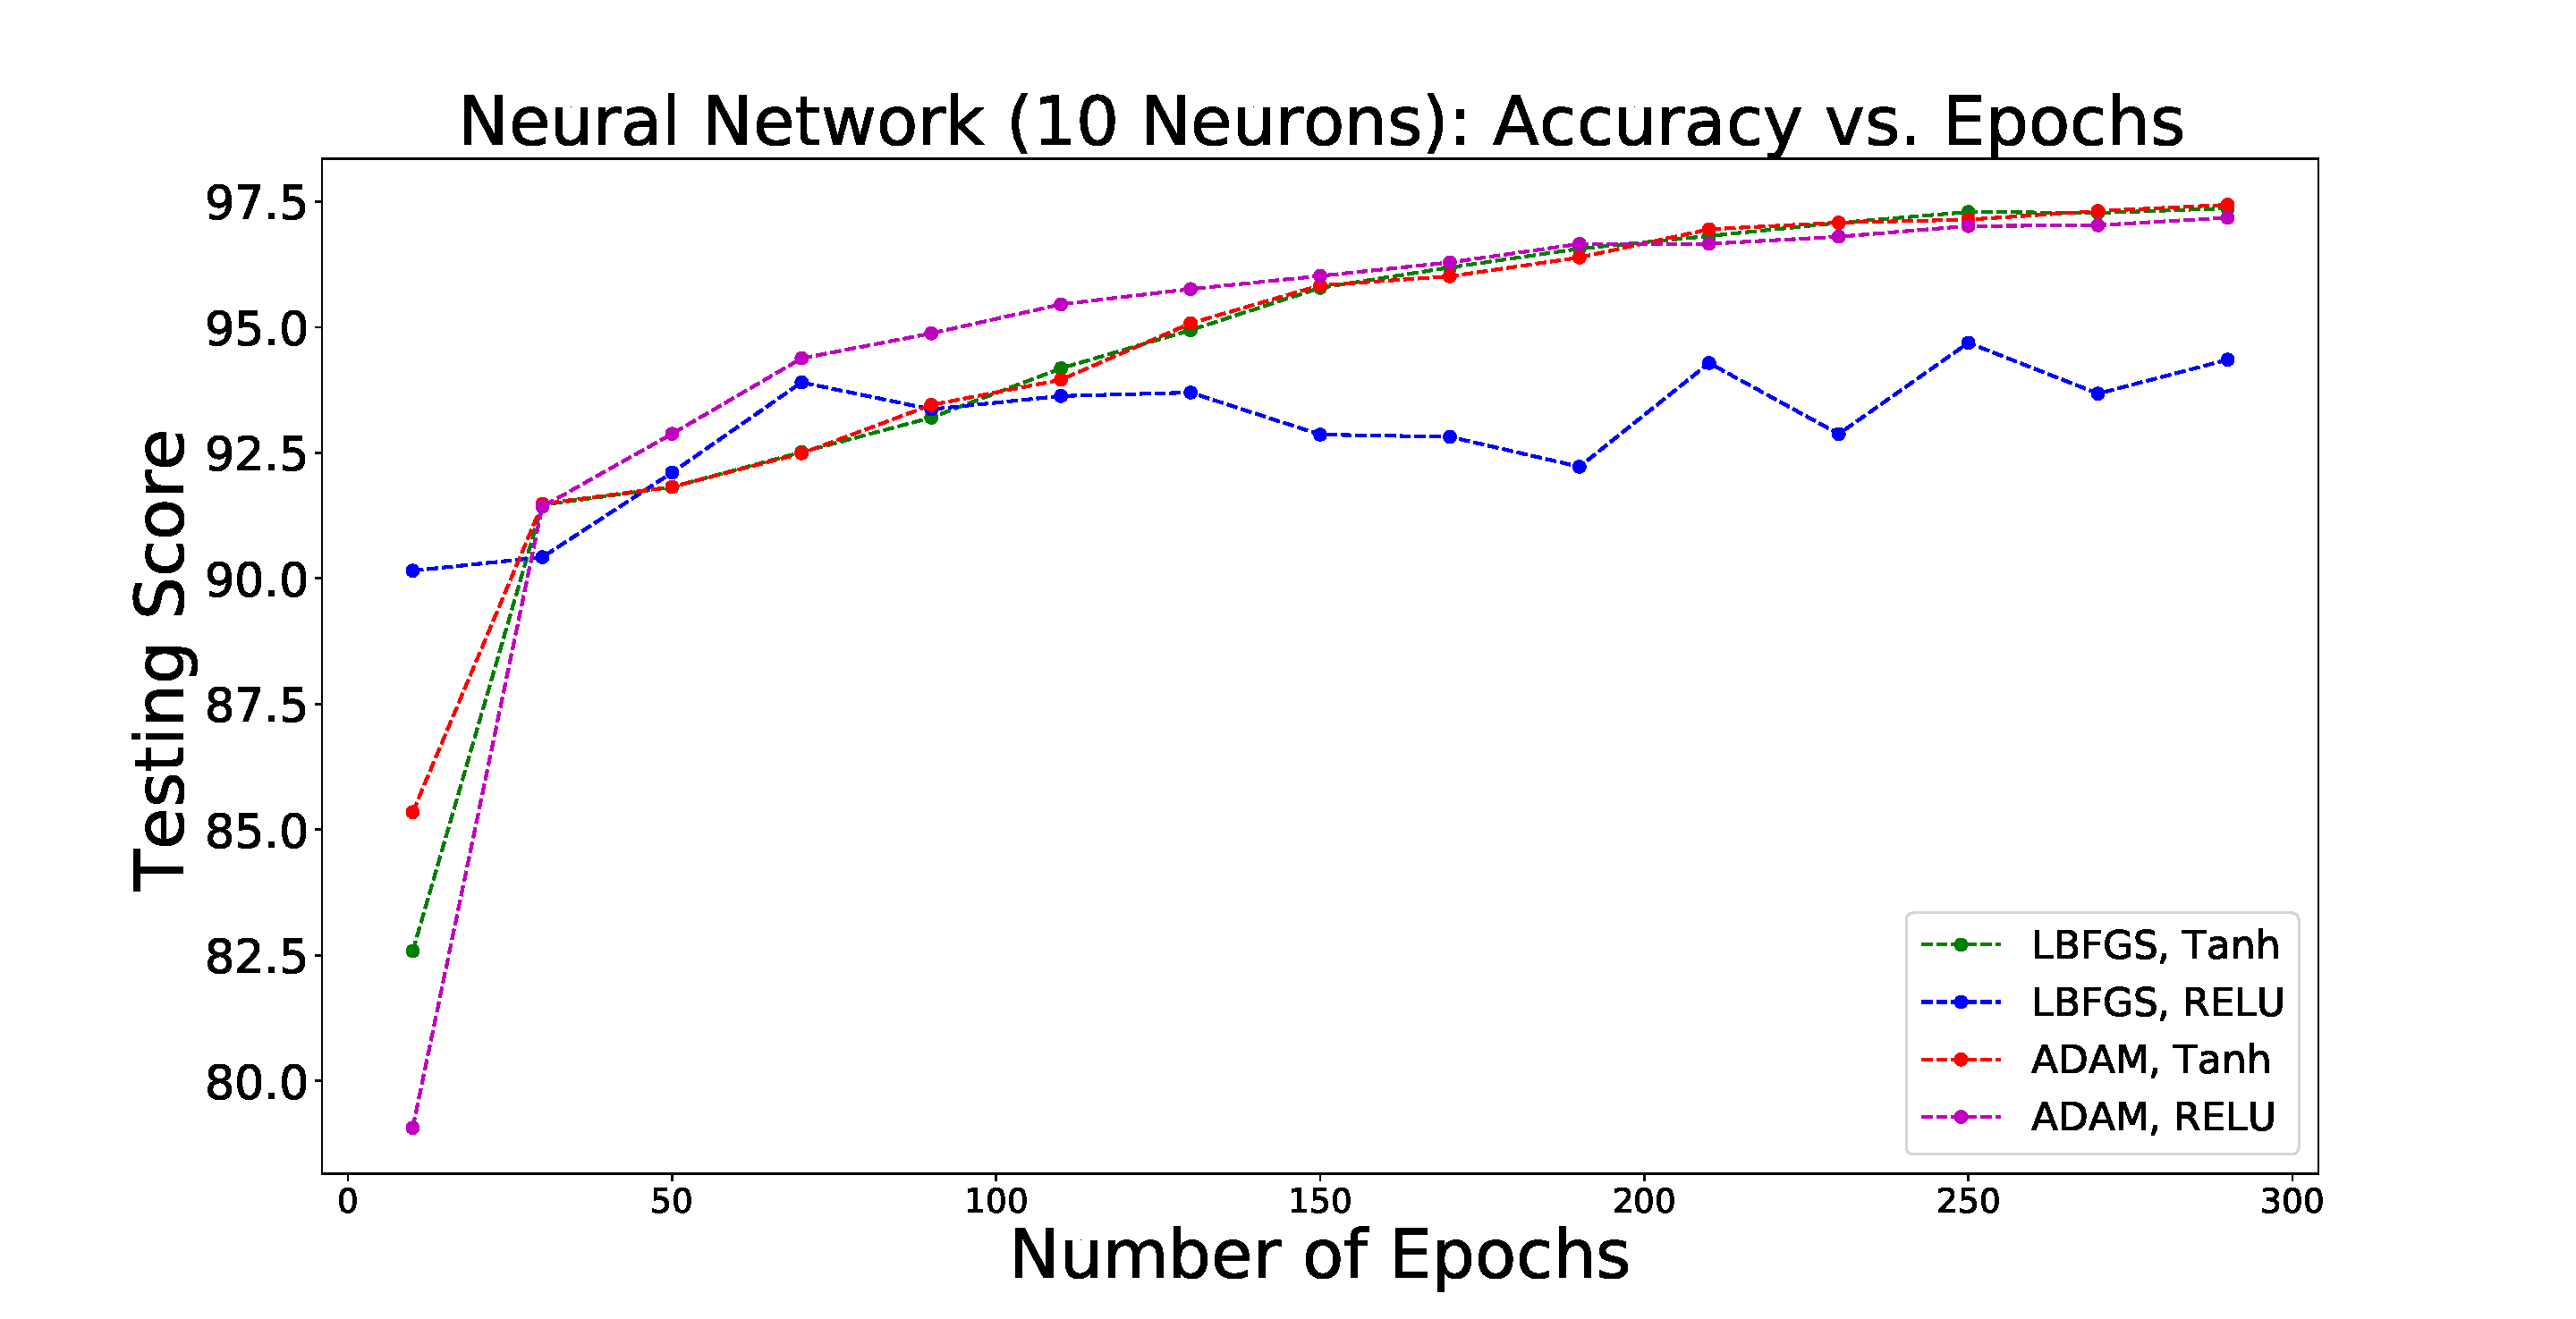
\includegraphics[width=0.5\textwidth]{plots/nn_epochs.pdf}
\caption{
Dependence on epochs for different solvers and activation function
}
\label{fig:NN_epochs}
\end{figure}

%The next step was to see the effect of multiple hidden layers and number of neurons on the accuracy. In this case we found no clear dependence, and it seems as though the network doesn't overtraiin even for a higher number of neurons. This could be explained by the less number of iterations. Higher number of hidden layers added nothing more to the accuracy and serve to only over-fit the data.\\


\begin{figure}[h]
%\centerin
\hspace*{-0.5cm}
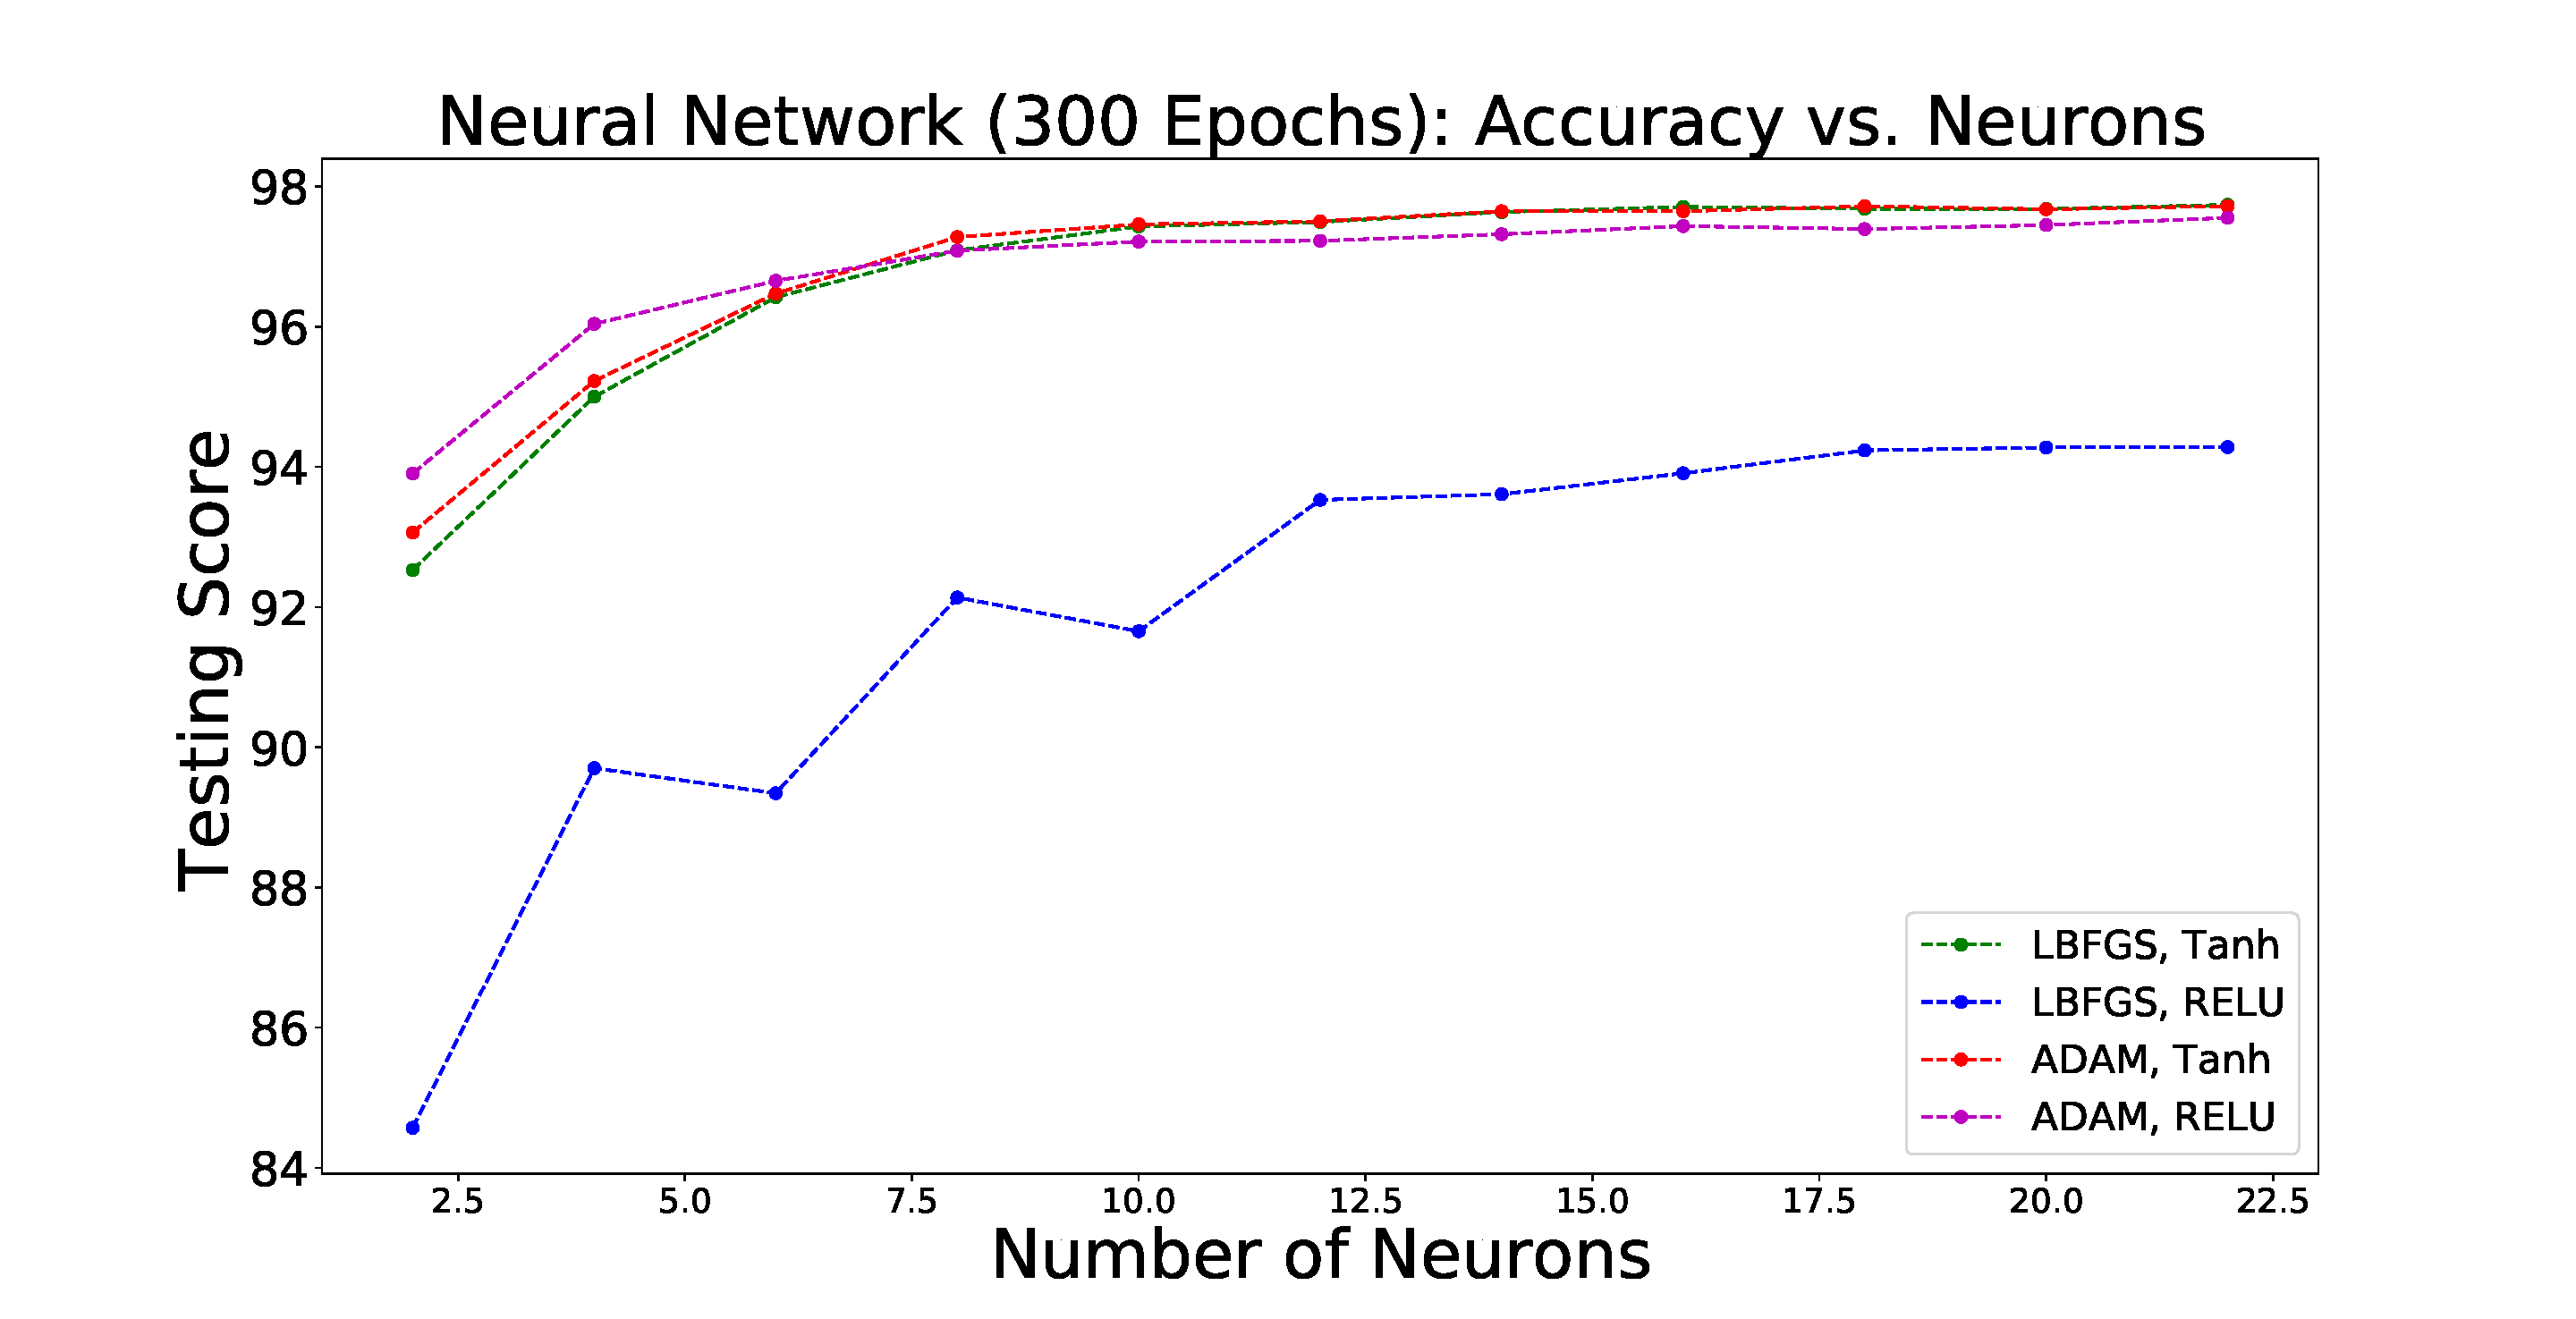
\includegraphics[width=0.5\textwidth]{plots/nn_neurons_300epochs.pdf}
%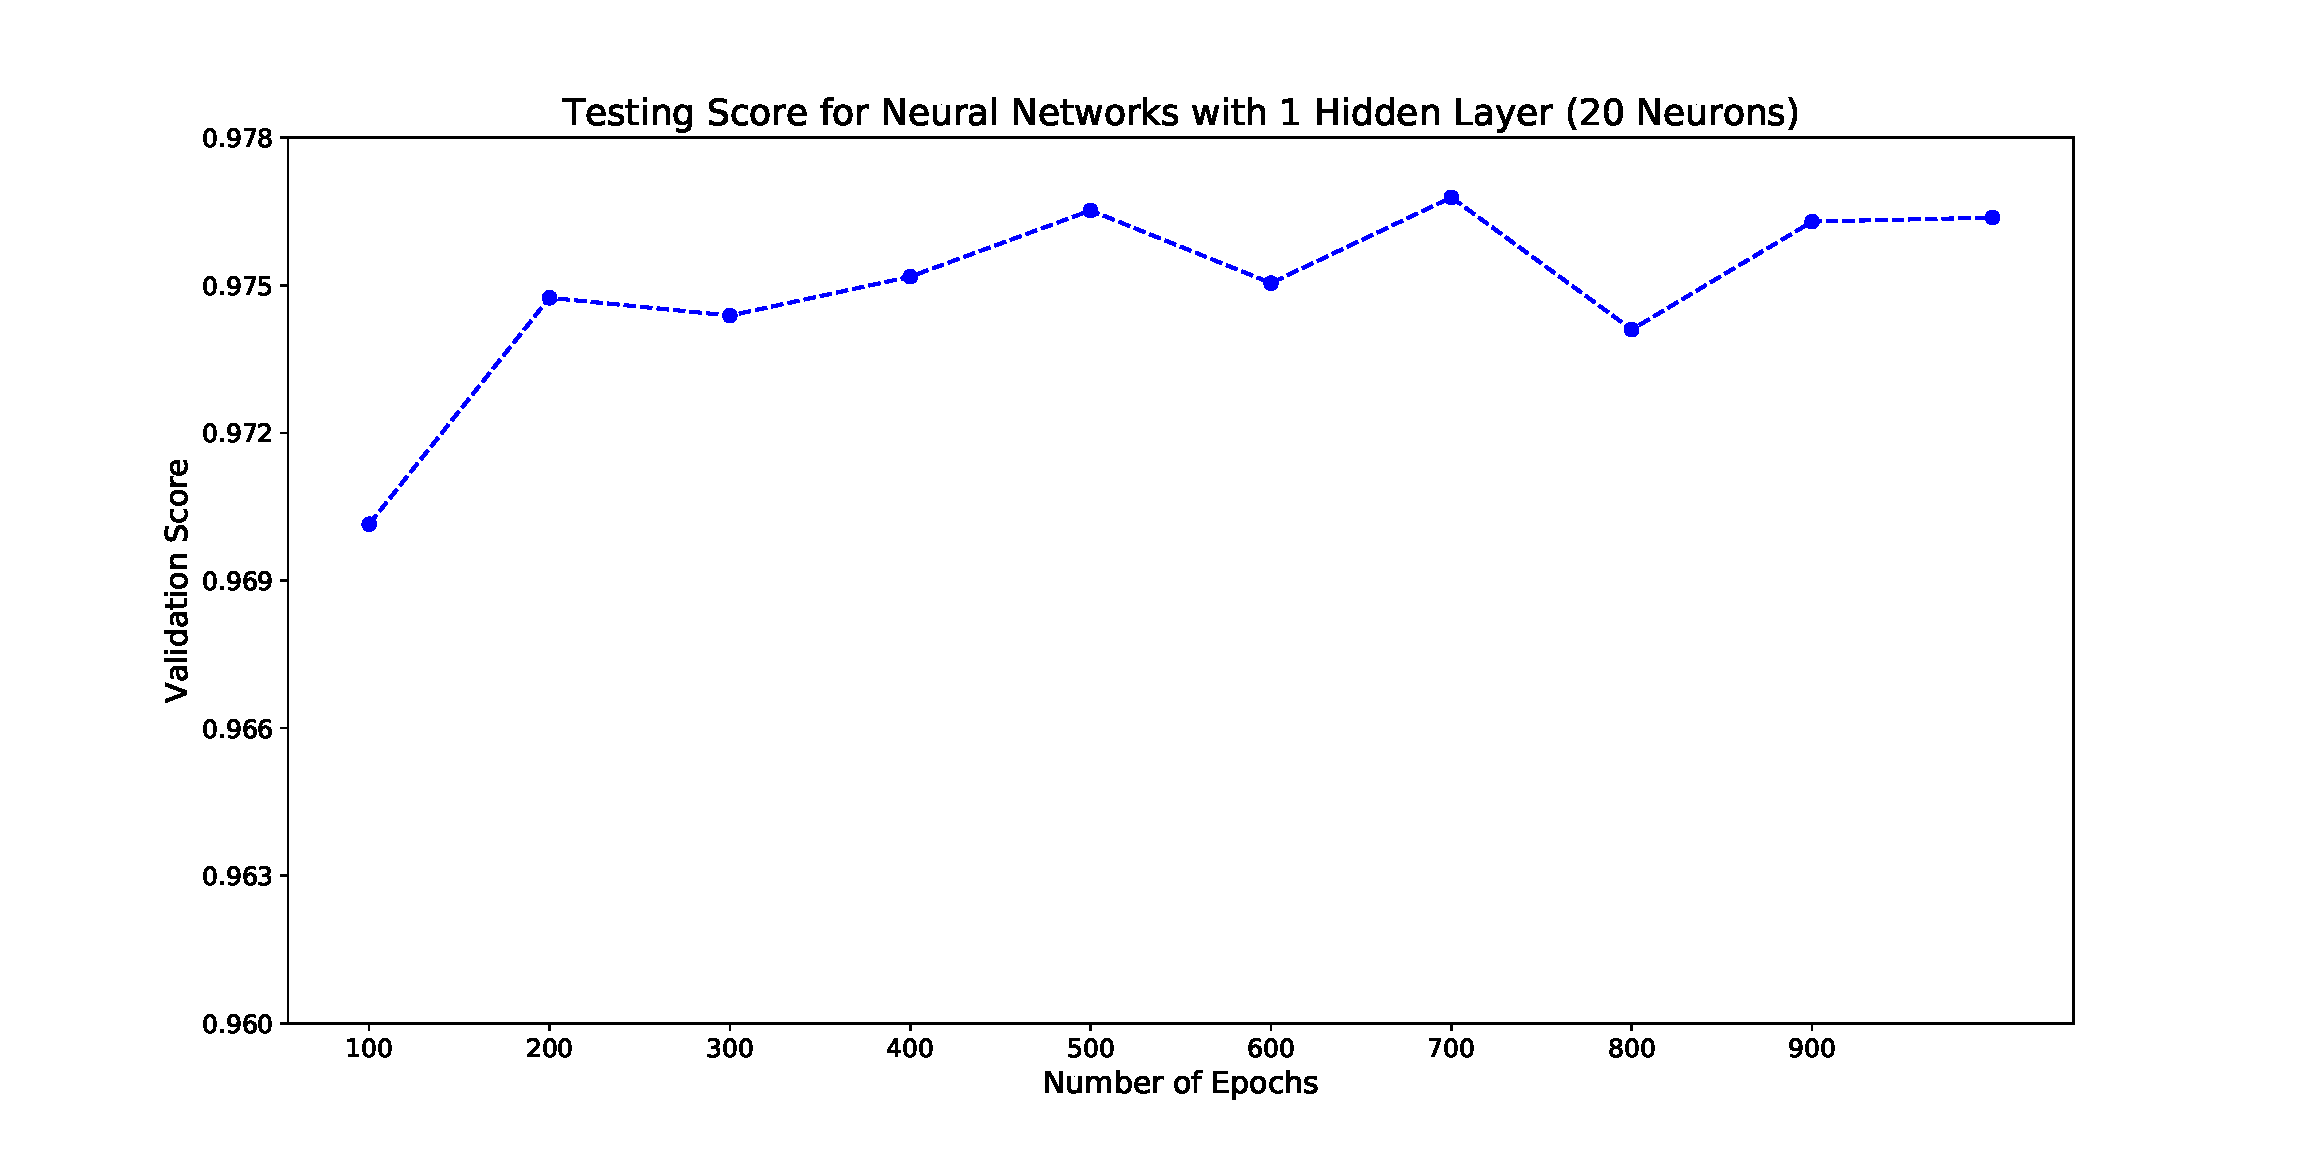
\includegraphics[width=\twopicsp\textwidth]{plots/epochsvsscore2_10seeds.pdf}
\caption{Dependence of accuracy on number of neurons for different models.}
%\dima{I'm not sure I understand where you use Tanh or RELU activations, if we have only one hidden layer with sigmoid activation (I guess) for classification?}}
\label{fig:NN_neurons}
\end{figure}

Domains for NN with only two input features are shown in Figure \ref{fig:NN_domains}.
\dima{As above, I don't think it makes sense to use more than 2 nodes in the hidden layer here, since there are only two input features.}


\begin{figure}[h]
%\centerin
\hspace*{-1.5cm}
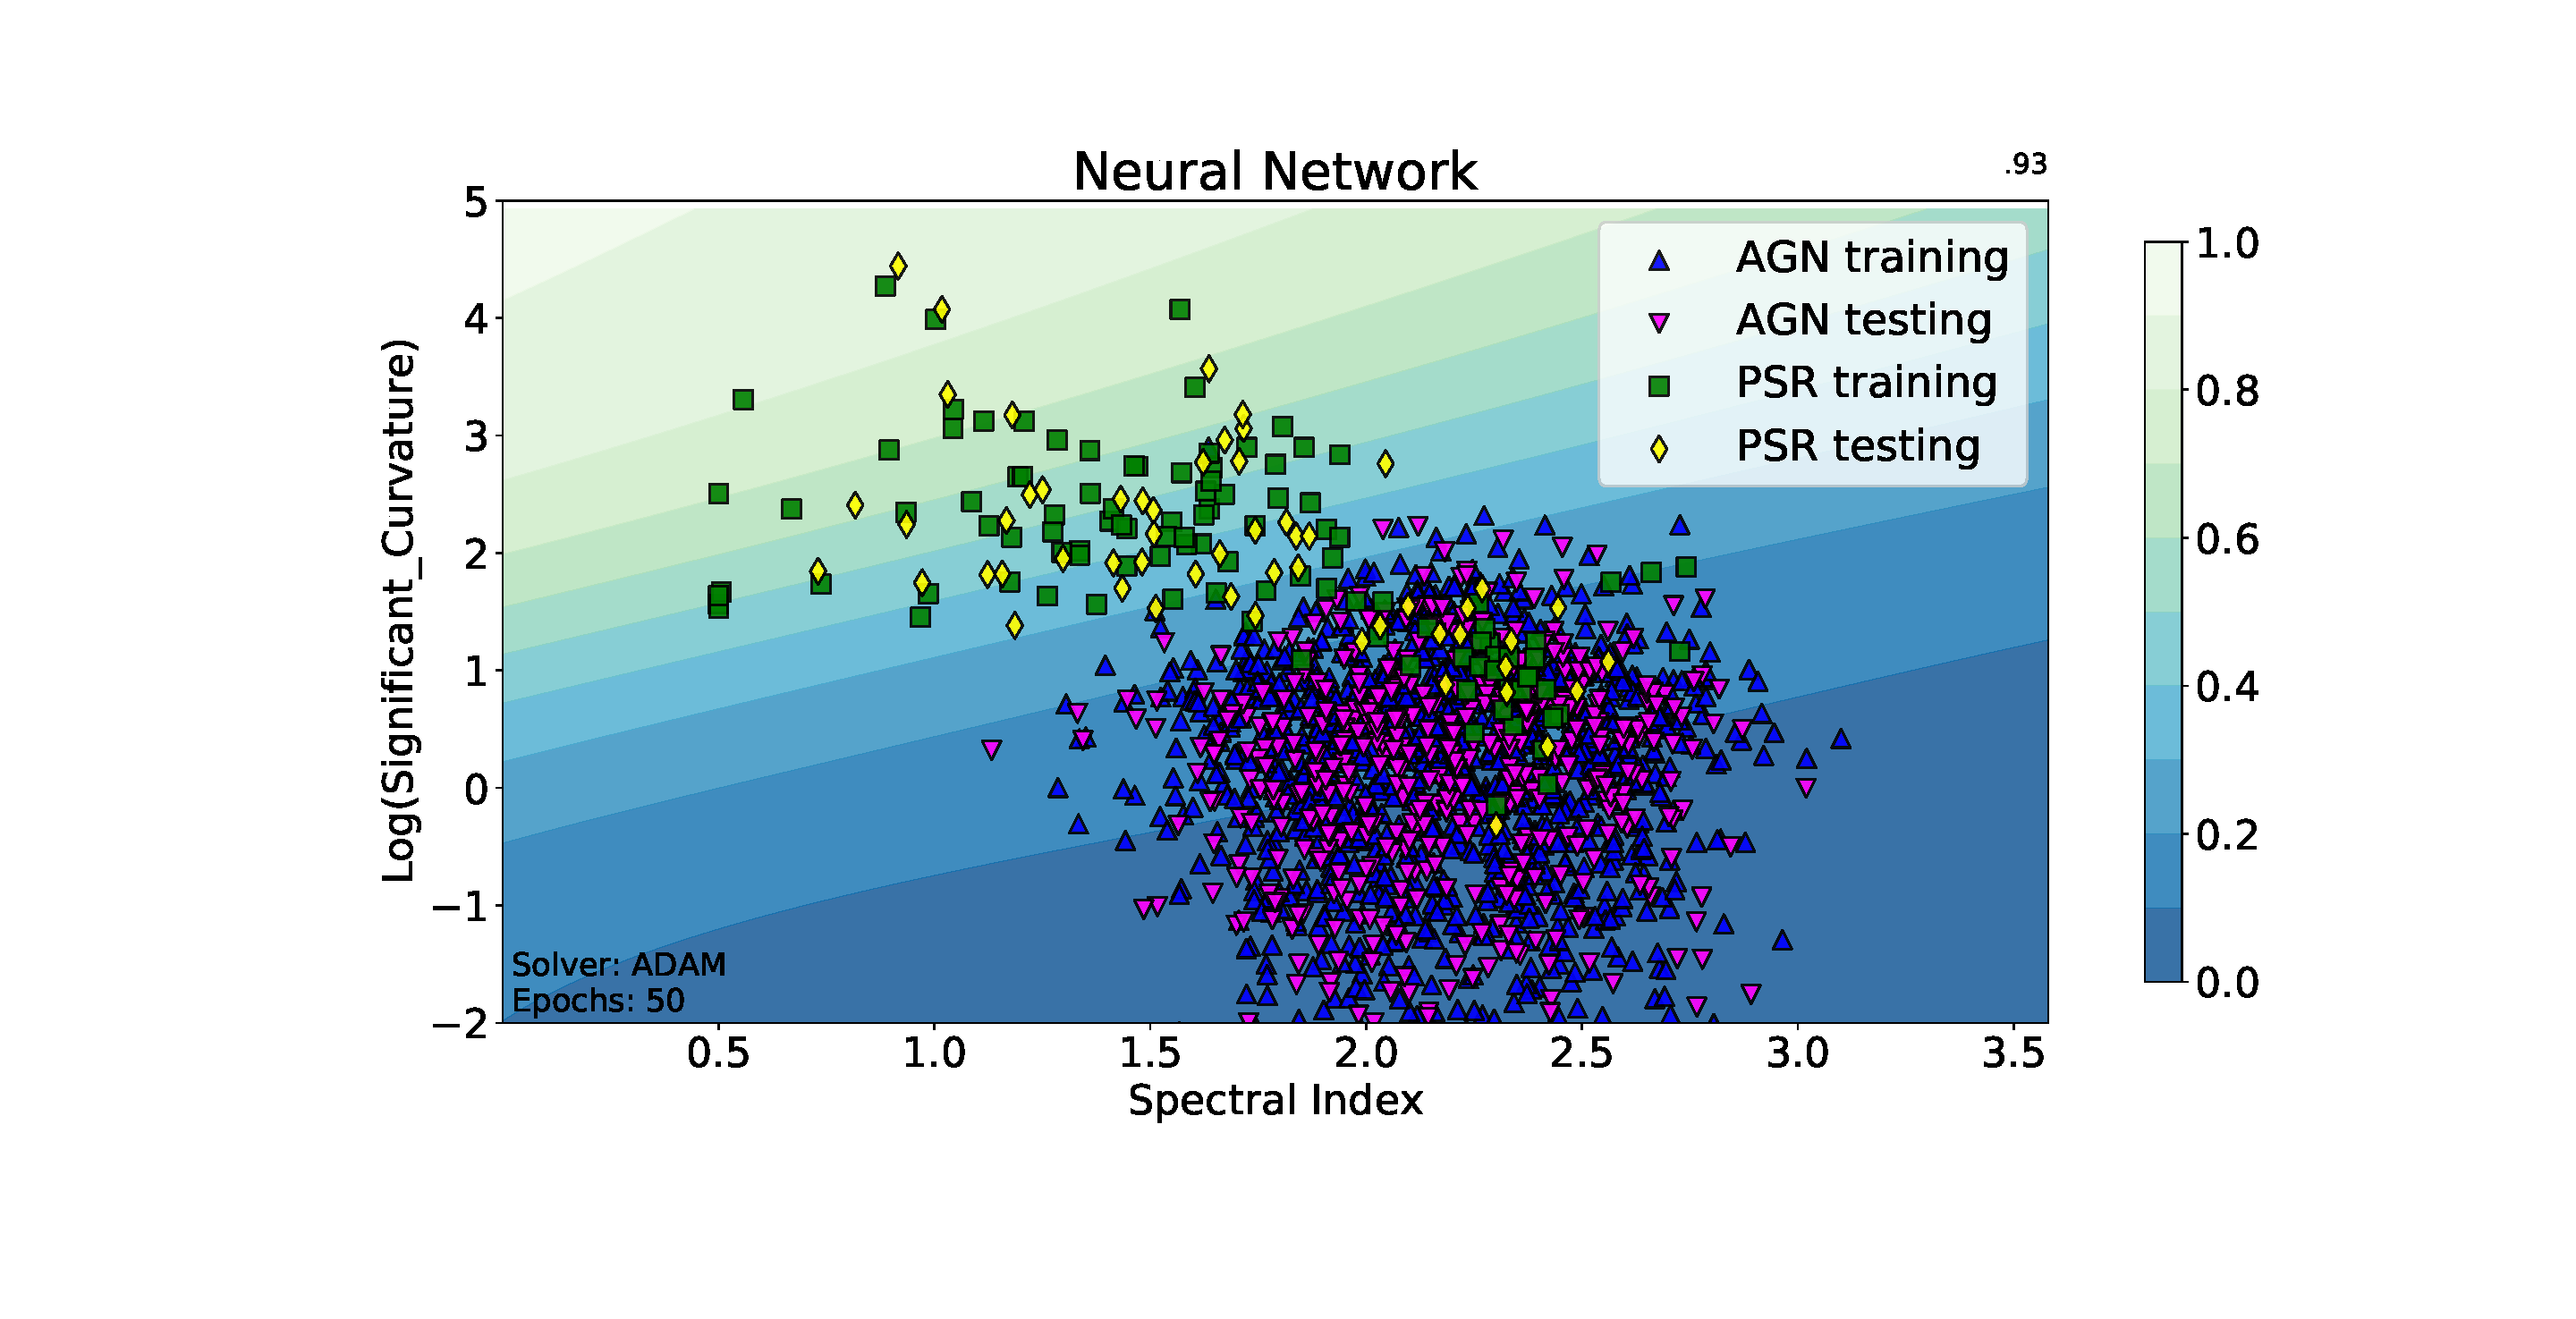
\includegraphics[width=0.6\textwidth]{plots/classification_domains/nn_adam_10_tanh_50_final.pdf}
\hspace*{-1.5cm}
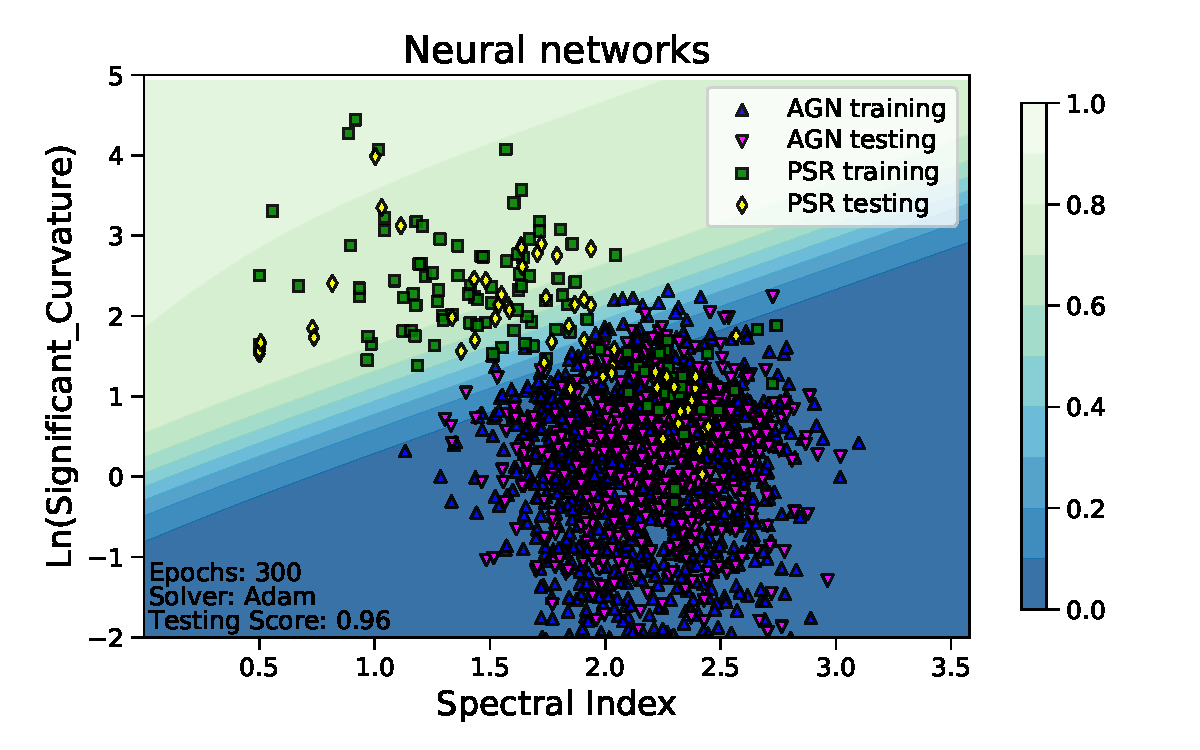
\includegraphics[width=0.6\textwidth]{plots/classification_domains/nn_adam_10_tanh_300_final.pdf}
\caption{Classification Domains for Neural Networks for the same complexity of 10 Neurons and tanh activation, using ADAM solver. }
\label{fig:NN_domains}
\end{figure}

\subsection{Boosted Decision Trees}

The free parameters for BDT algorithms are similar to RF algorithms: the number of trees and the maximal depth.
We will use the gradient boosting algorithm for the construction of BDT.
The classification is performed by a weighted average of trees, where the trees are constructed recursively in order to better address 
misclassifications from the previous step. The new trees are added with an additional parameter $\nu$ called learning rate.
We will use learning rate $\nu = 0.3$.
\dima{I'm not sure we need to discuss the learning rate, since we haven't done so in, e.g., neural networks}
Dependence of the accuracy on tree depth is shown in Figure \ref{fig:BDT_depth}. The plot shows that depth of 2 and 100 trees is near the optimal limit. 
%\dima{Which depth do we use for the final algorithm, it looks like depth 2 gives the best results. What about depth = 1?}

\begin{figure}[h]
%\centerin
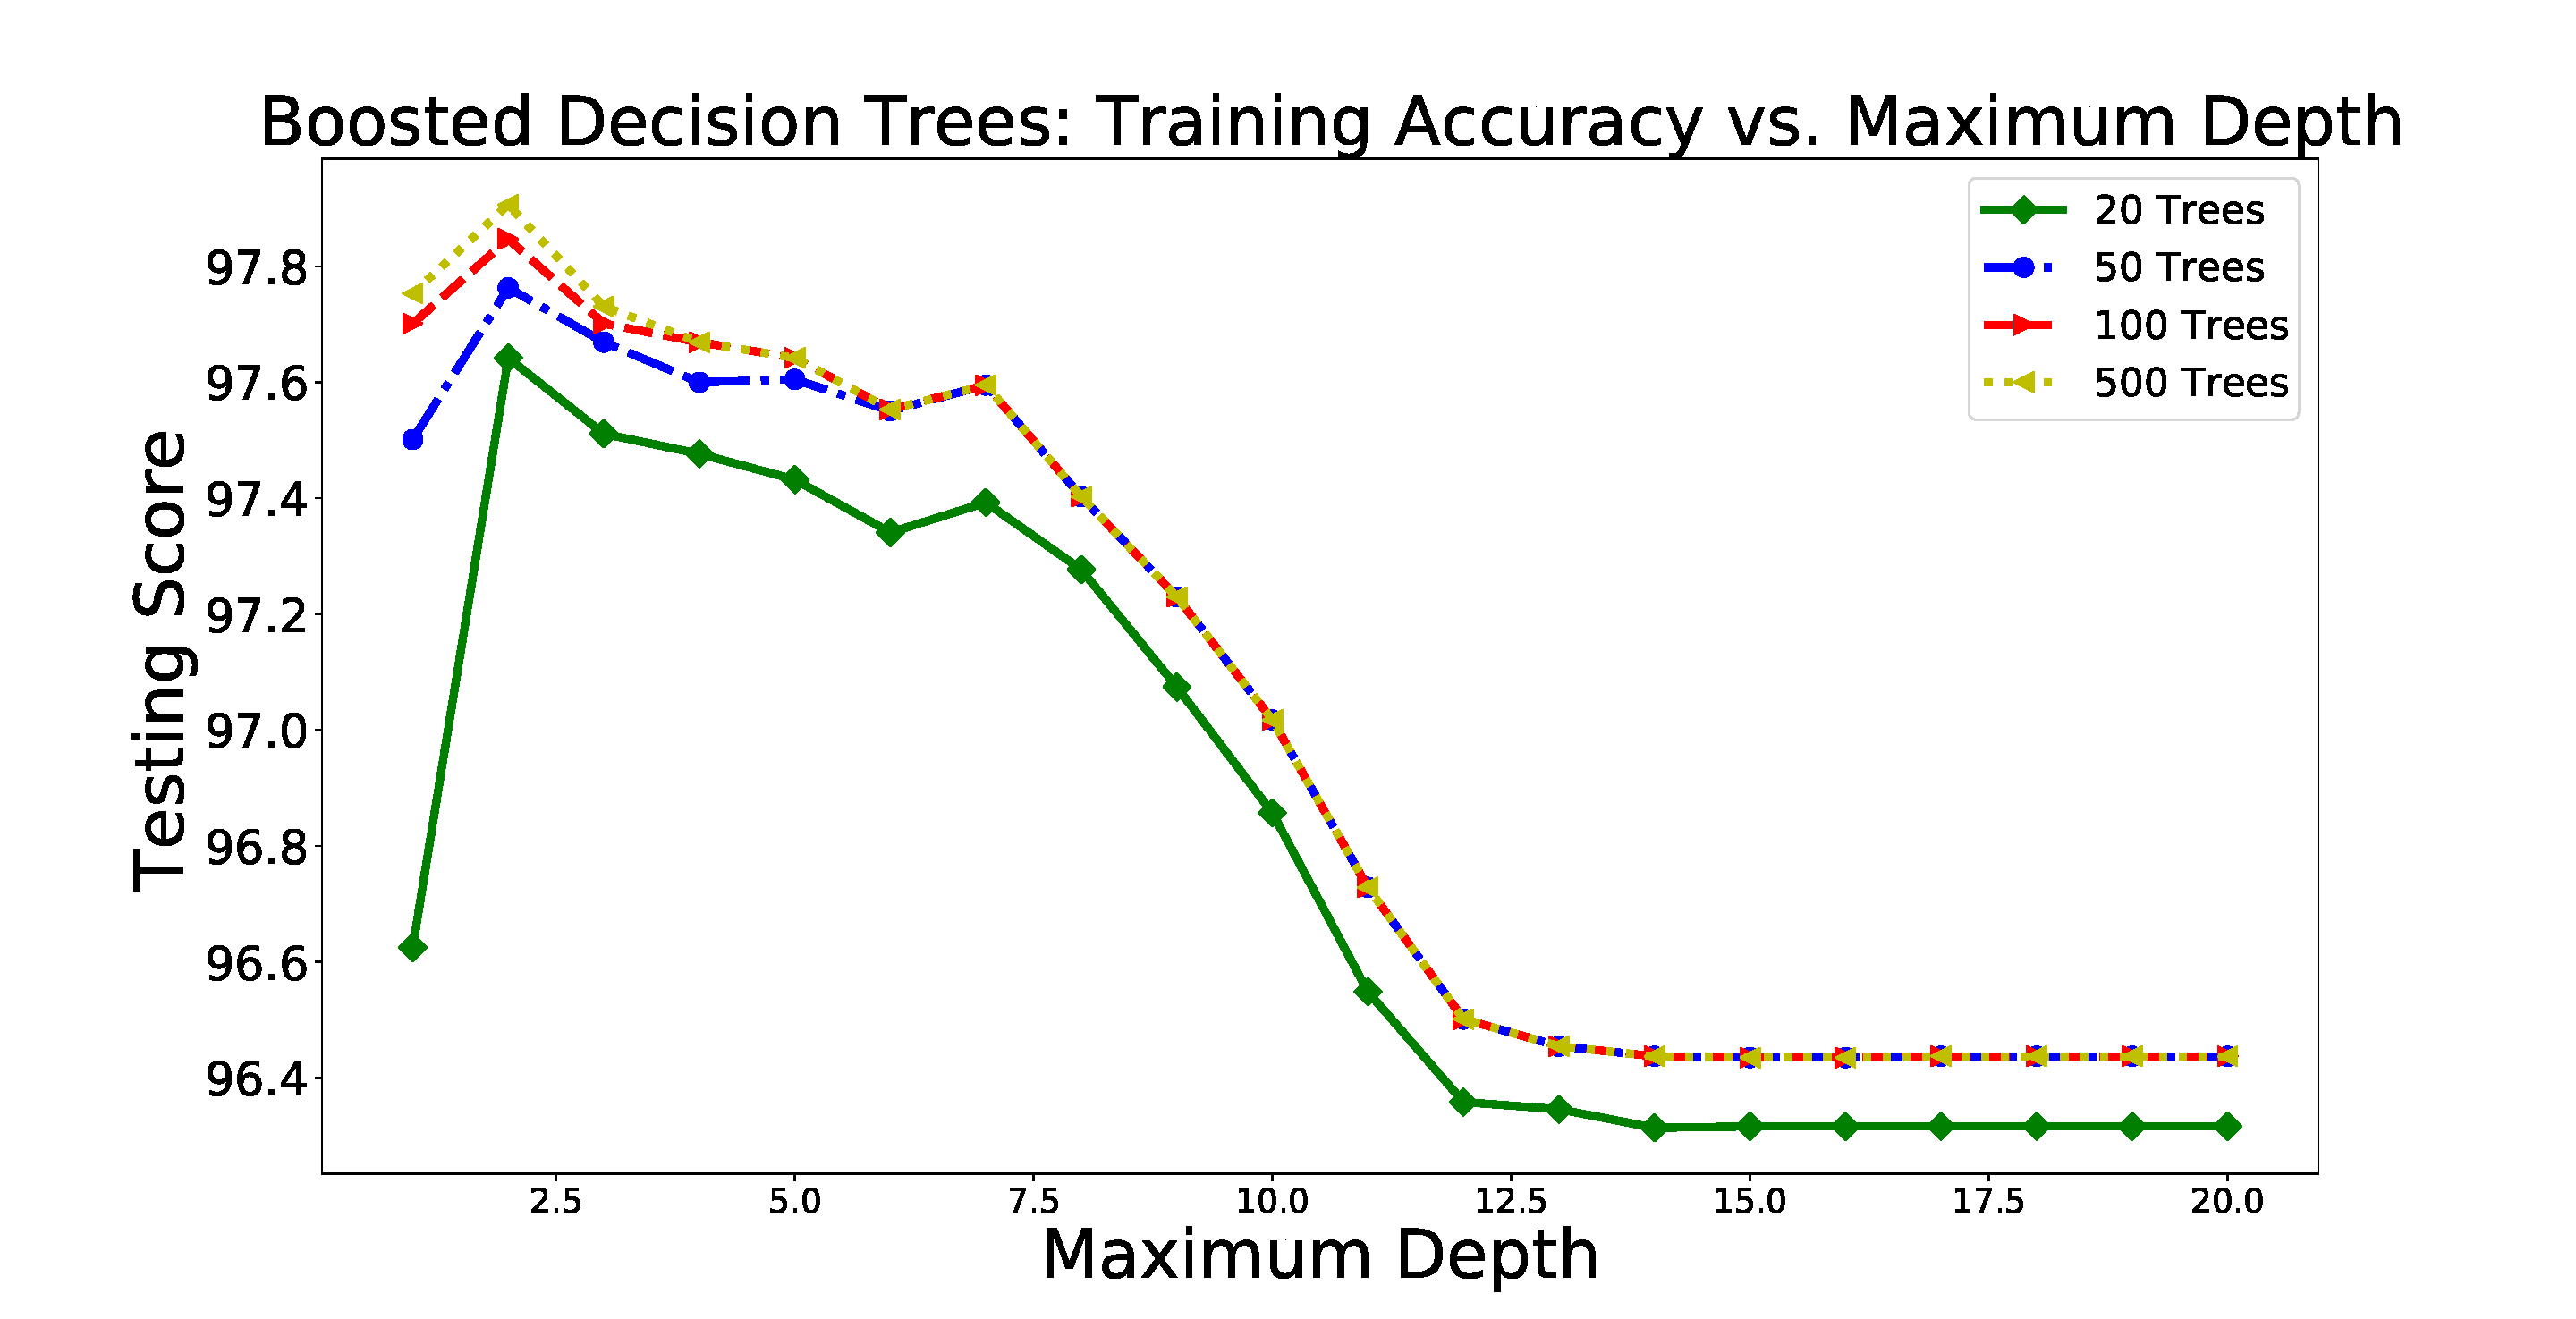
\includegraphics[width=\twopicsp\textwidth]{plots/bdt_train.pdf}
%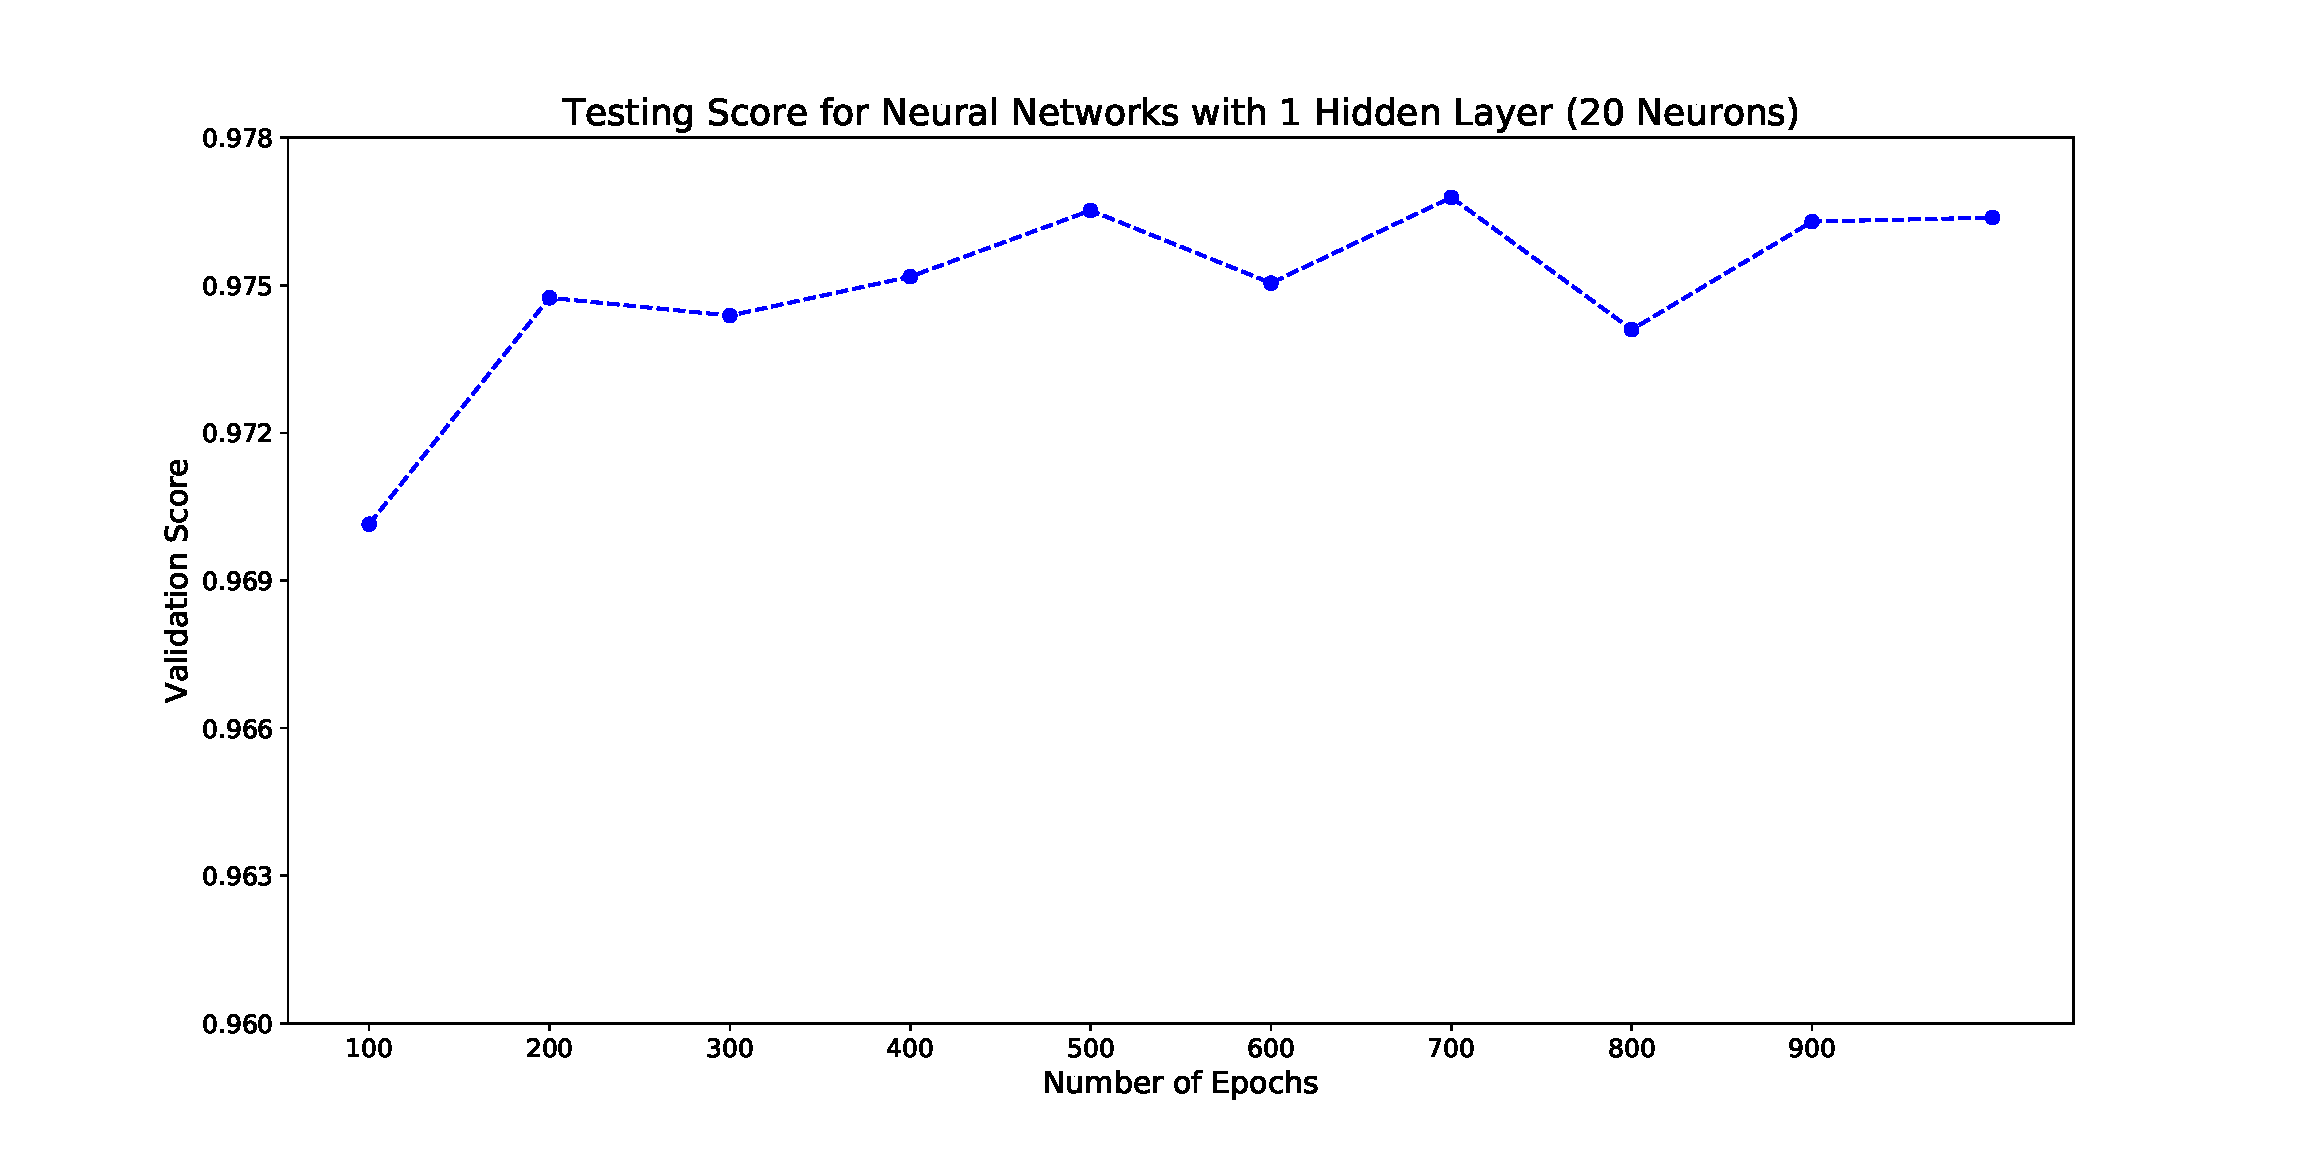
\includegraphics[width=\twopicsp\textwidth]{plots/epochsvsscore2_10seeds.pdf}
\caption{Dependence of BDT accuracy on maximum depth}
\label{fig:BDT_depth}
\end{figure}

The Classification domains in case of two features for the maximal depth of 3 and 15 is presented in Figure \ref{fig:BDT_domains}. The greater than a percent decrease in the accuracy from a max depth of 3 to a max depth of 15 can be explained by the domains, where we see a pattern of almost over-fitting the data. While for 2 features the decrease is small, it should increase as we increase the number of features, with a lower complexity network being enough for a good accuracy.
%Boosted Decision Trees again show a similar effect as Random forests in their classification, and have a significant difference when the model complexity is changed.

\begin{figure}[h]
%\centerin
\hspace*{-1.5cm}
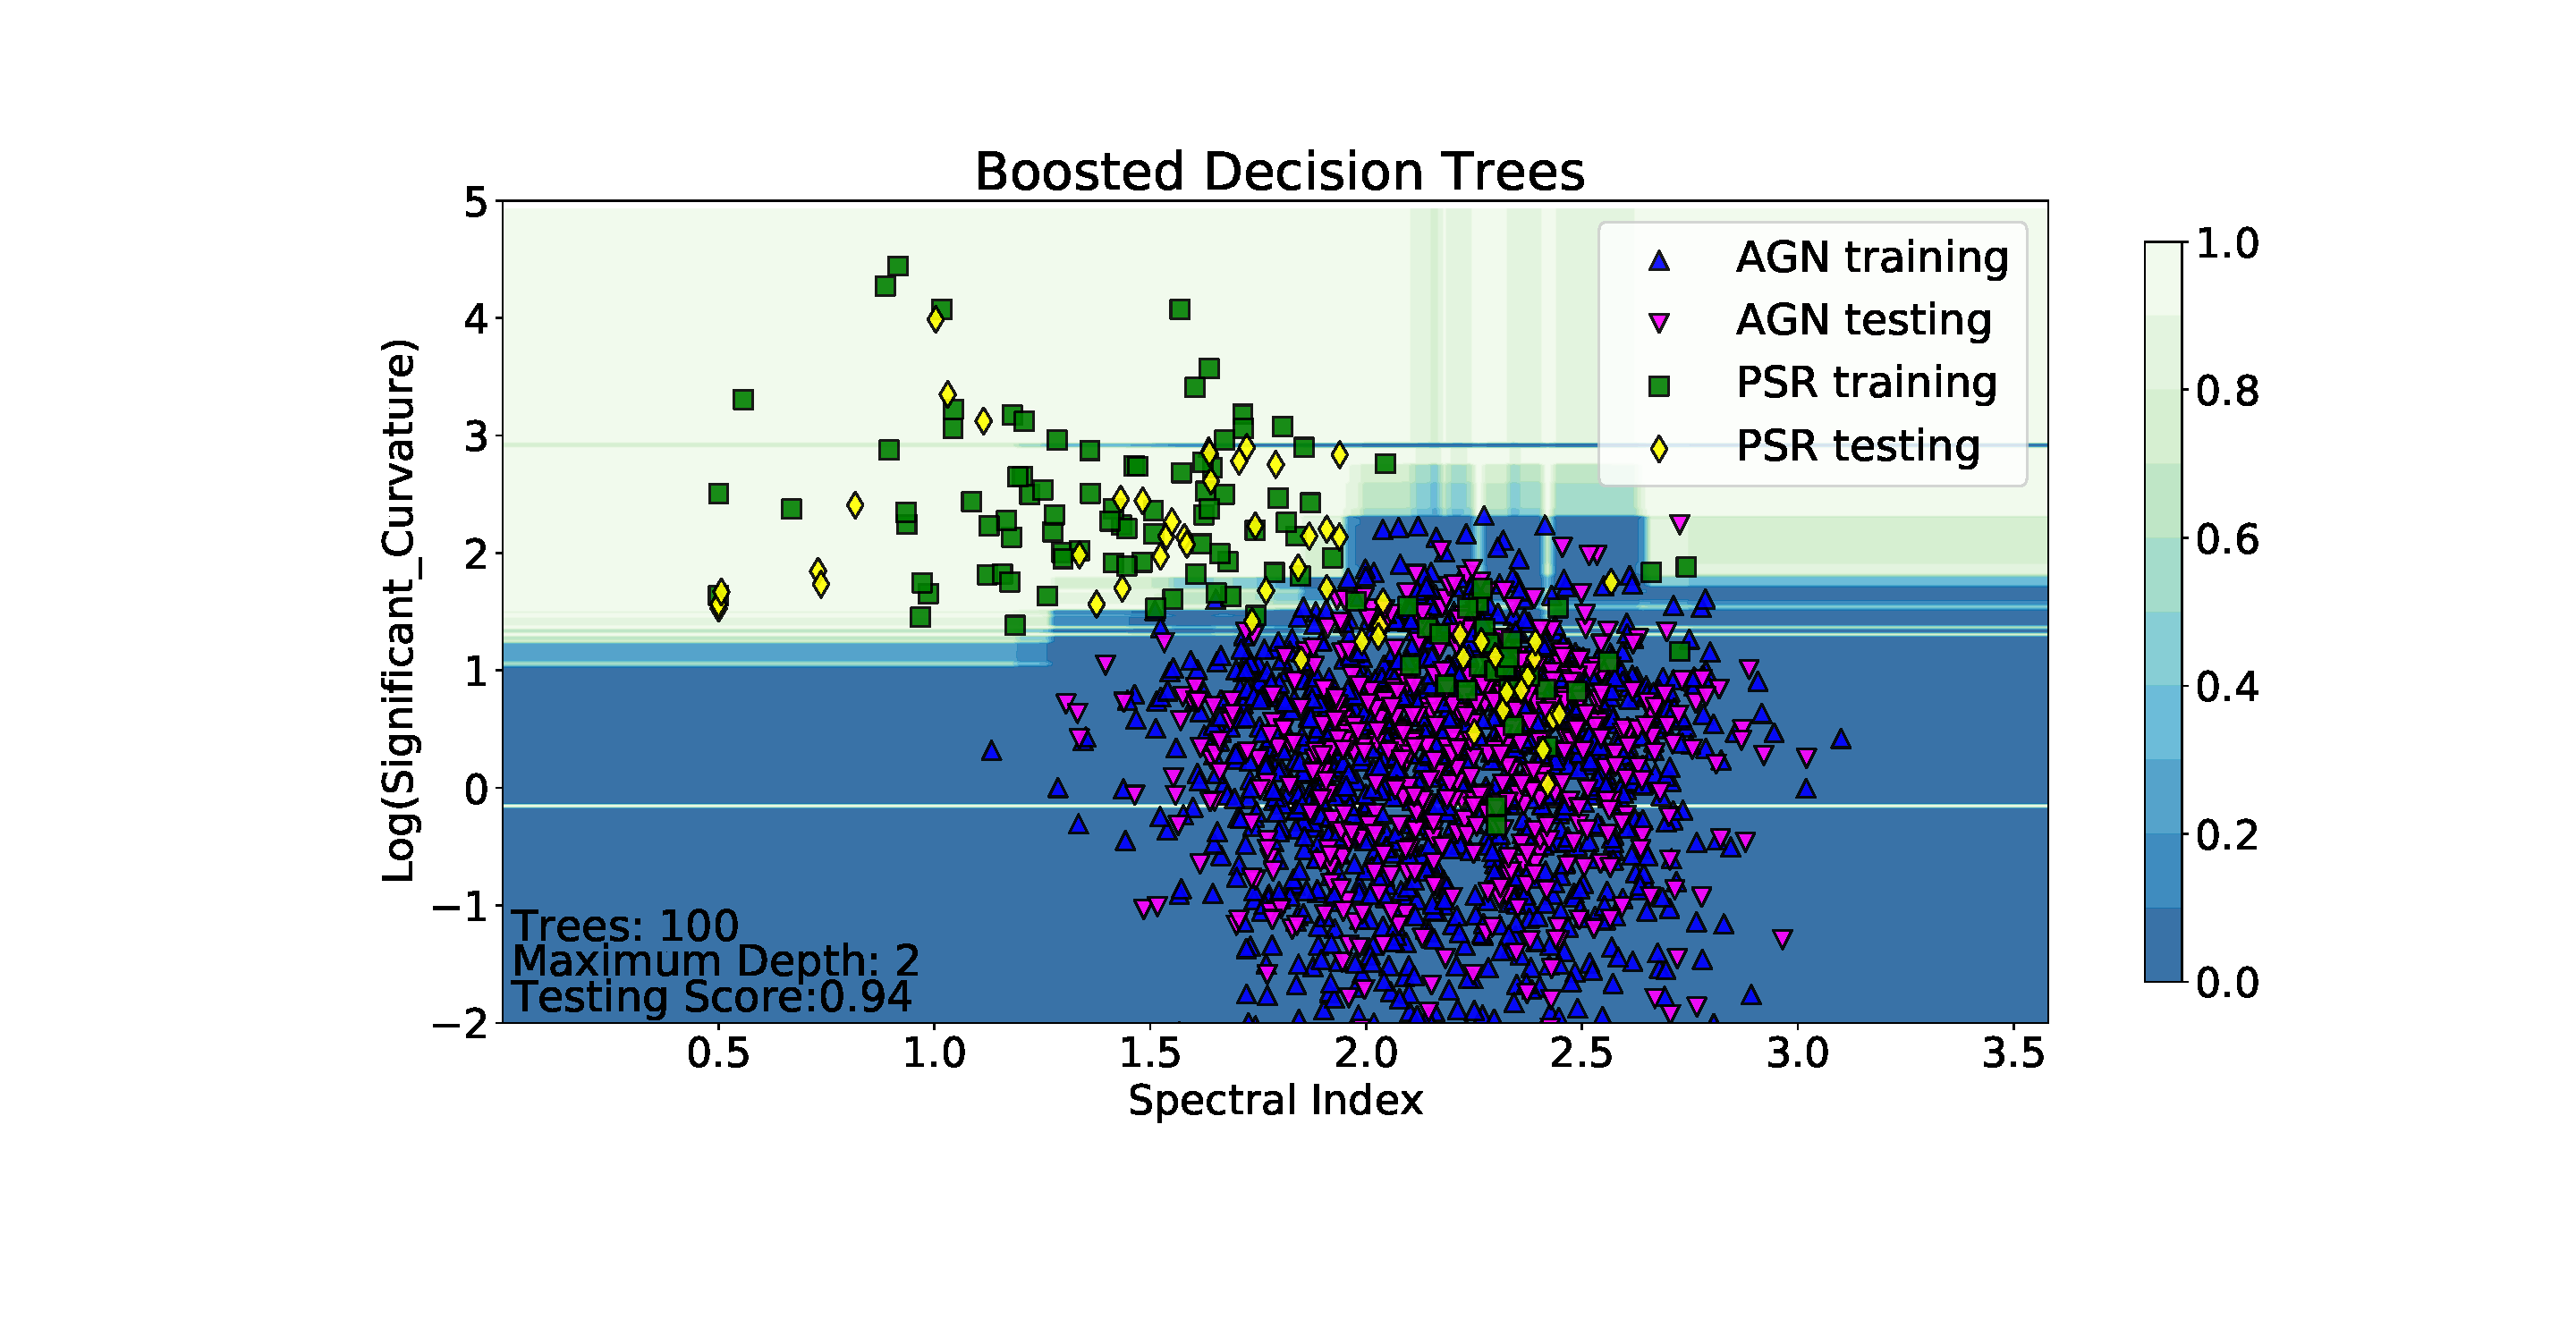
\includegraphics[width=0.6\textwidth]{plots/classification_domains/bdt_100_2.pdf}
\hspace*{-1.5cm}
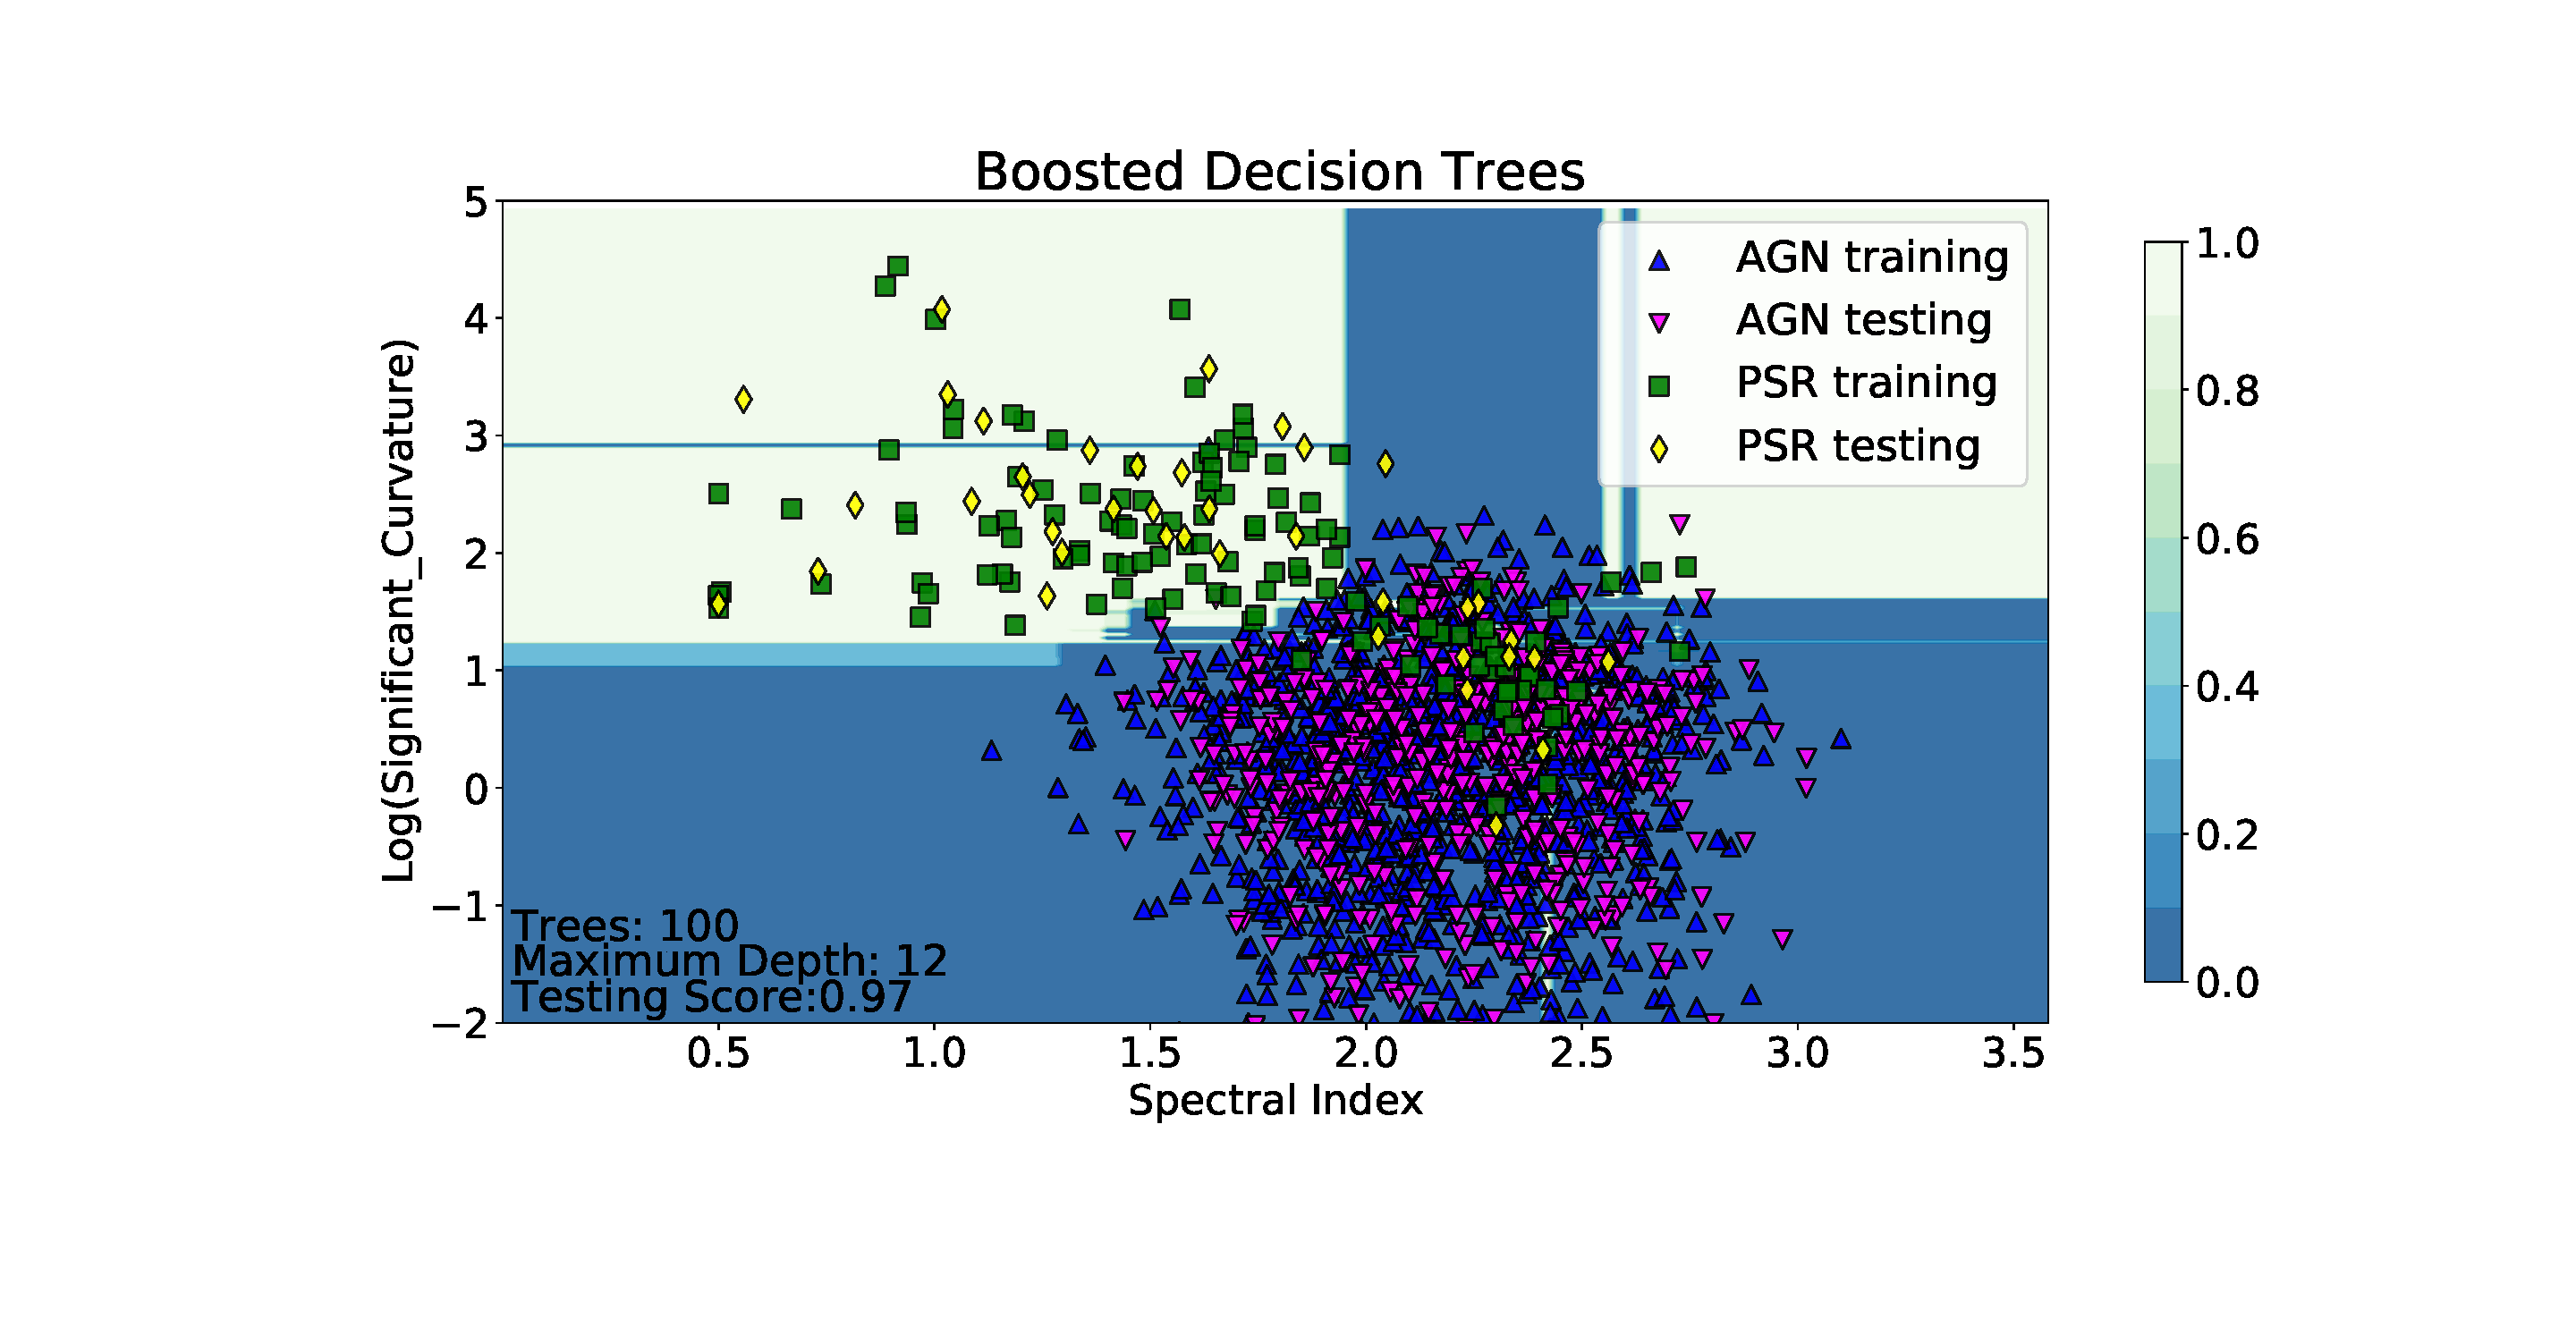
\includegraphics[width=0.6\textwidth]{plots/classification_domains/bdt_100_12.pdf}
\caption{Classification Domains for BDT}
\label{fig:BDT_domains}
\end{figure}


\begin{comment}
Is learning rate equivalent to the 
Boosted Decision Trees or Gradient boosting algorithms are similar to Random Forests, having number of trees and maximum depth as parameters. However, here we also have the learning rate which specifies how fast (or slow) a model learns. This parameter is quite important, as a high value will converge faster but under-fit, whereas a lower value will over-fit. Therefore, we first chose an architecture of (50,6) and (20,6) to look at the dependence on number of trees. Here we found that low learning rate is preferred, and the maximum accuracy is reached at around 0.1-0.3. After a maximum the accuracy falls drastically since the BDT doesn't have enough time to learn properly. However, after a certain maximum depth, this doesn't hold true anymore irrespective of the number of trees. In this case, the BDT is complex enough that it learns fast and the accuracy doesn't fall even for higher learning rates. The figures below illustrate this.\\



\begin{figure}[h]
%\centerin
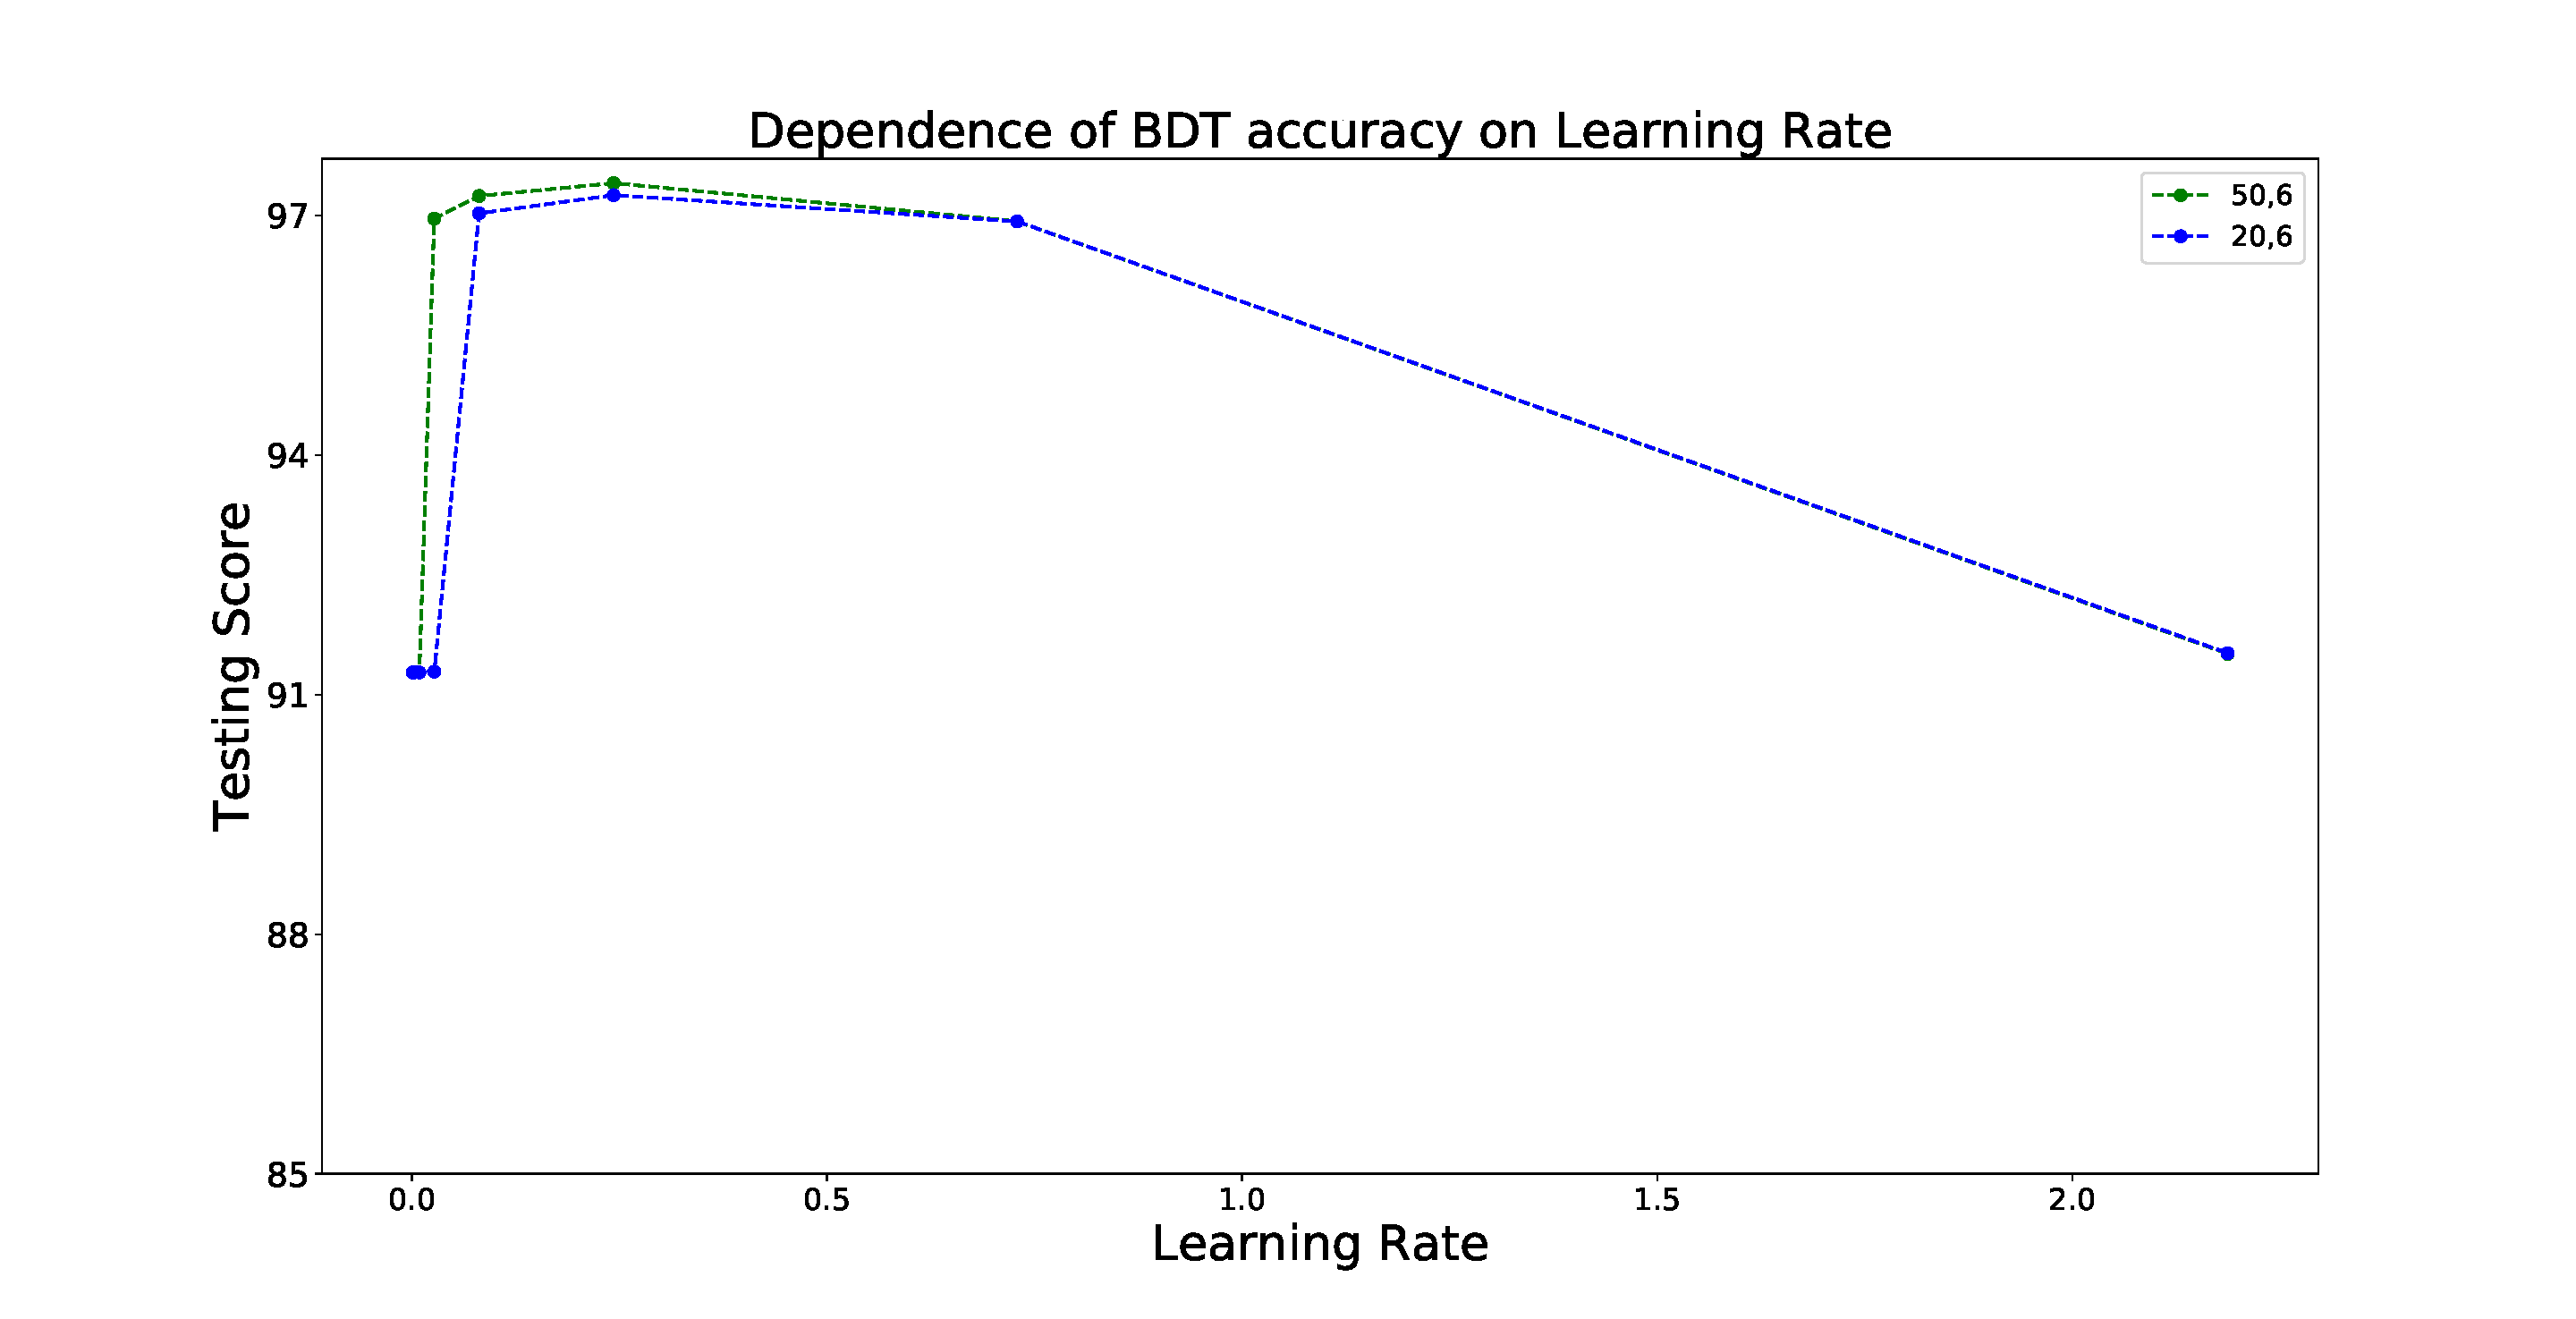
\includegraphics[width=\twopicsp\textwidth]{plots/lr.pdf}
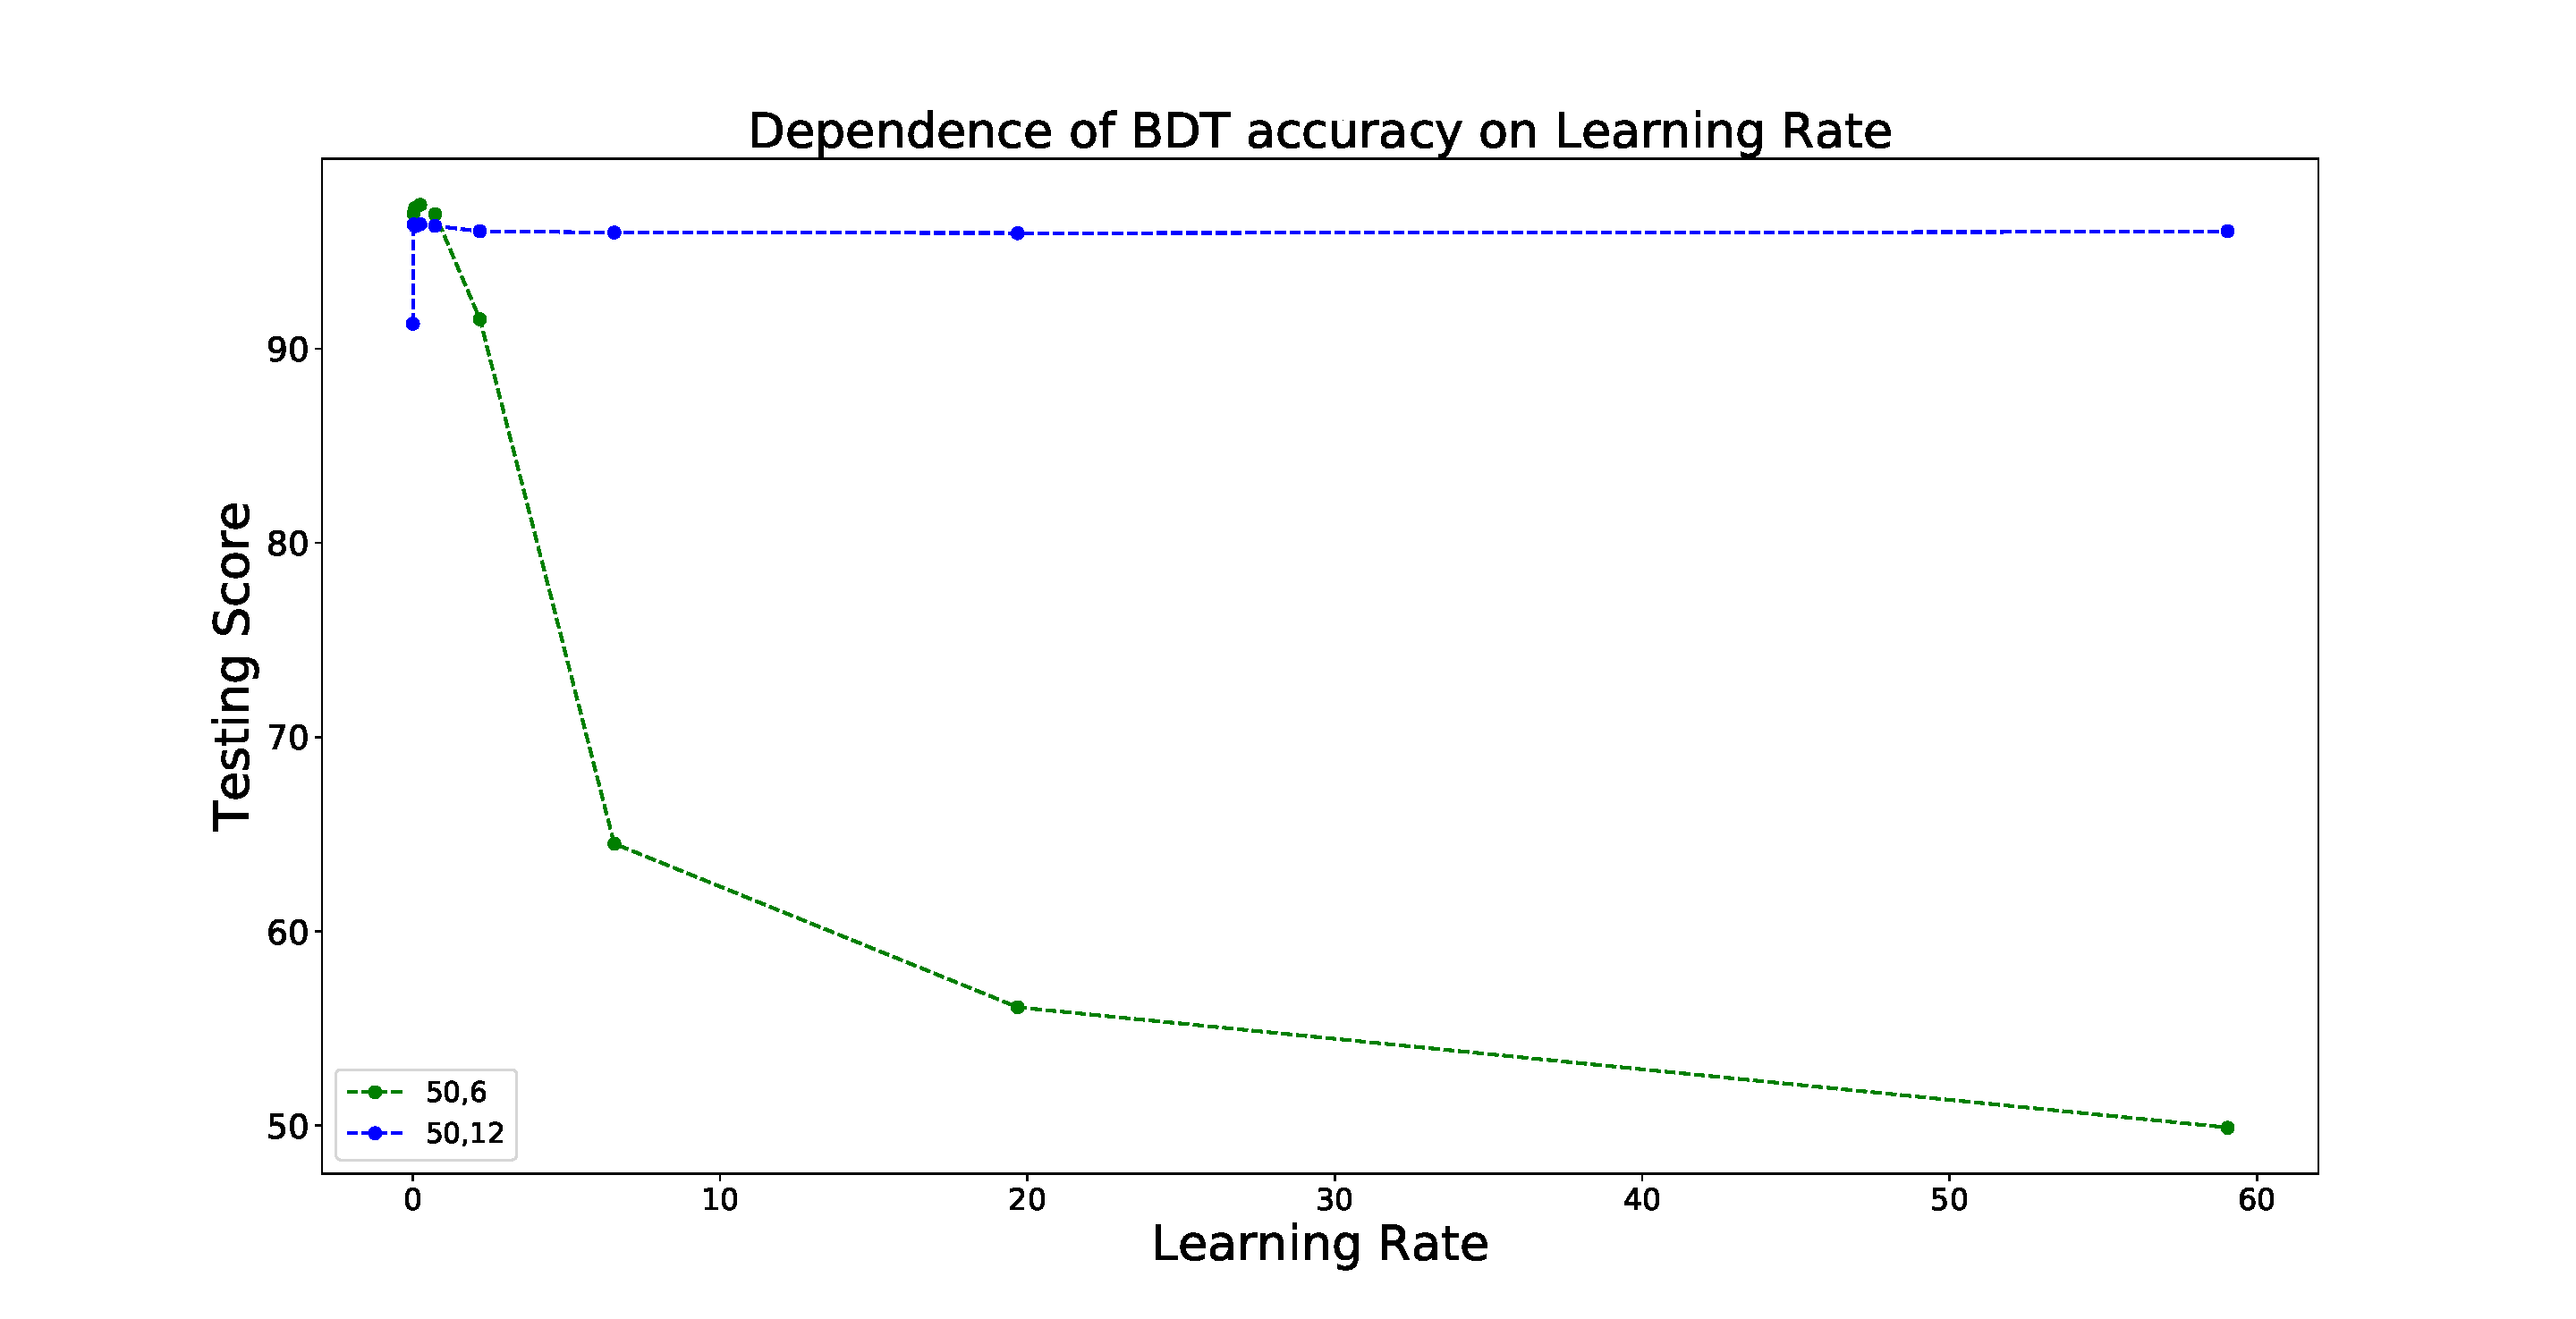
\includegraphics[width=\twopicsp\textwidth]{plots/lr3.pdf}
\caption{Dependence of BDT accuracy on learning rate with number of trees and maximum depth kept constant.
\dima{I'd include the name of the algorithm in the filenames, so that we can easier find them in the folder. ``lr'' sounds more like logistic regression.}}
\label{fig:BDT_learning_rate}
\end{figure}
\end{comment}




\subsection{Logistic Regression}

Logisitc Regression parameters include maximum iterations, tolerance, and a regularization parameter. In the figure below on can see that iterations change the accuracy only for the saga solver, and both lbfgs and liblinear are unchanged. The latter are faster algorithms good for smaller datasets like ours. Furthermore for our data set there is no strict dependence on the tolerance and after a threshold vale the regularization also produces the same result.
%\dima{Which parameters do we use for the final algorithm? For some set of parameters, the LR should be equivalent to NN in our case,
%in particular, the domains should be exactly the same (up to numerical convergence). 
%We can discuss several solvers, but for plots and further calculations I'd suggest to choose one solver and use only it, 
%I'm not sure if many people would be interested to see a dependence on the solver.}


\begin{figure}[h]
%\centerin
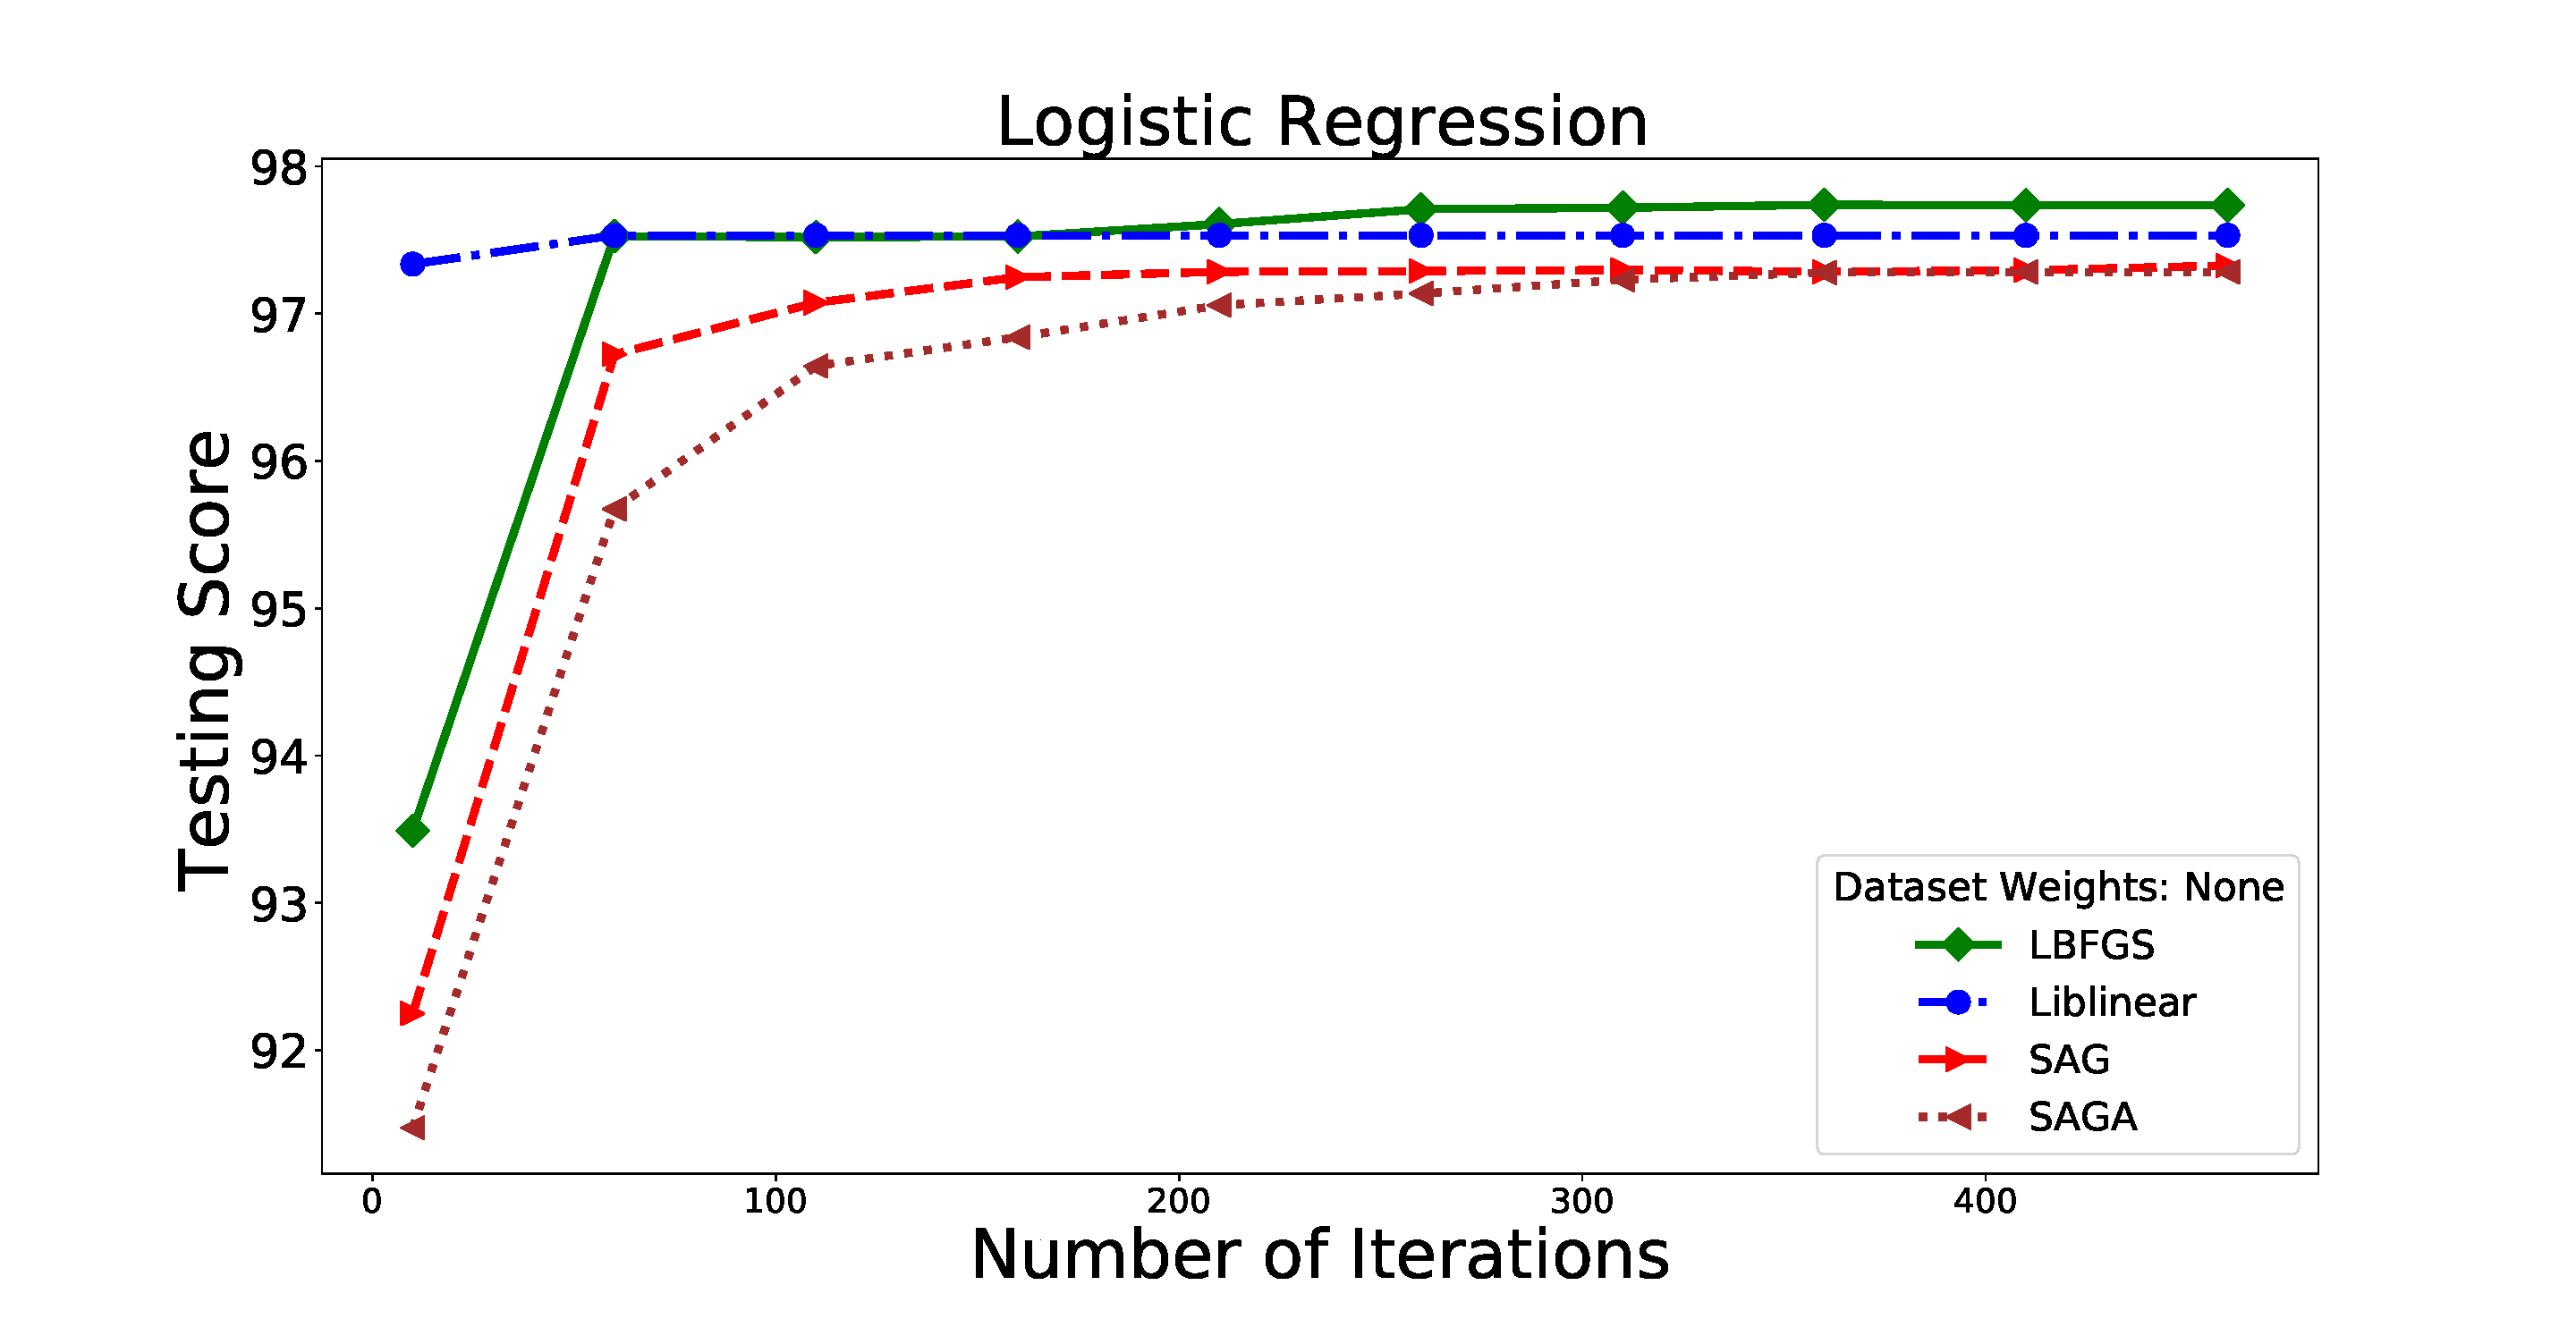
\includegraphics[width=\twopicsp\textwidth]{plots/lr_train.pdf}
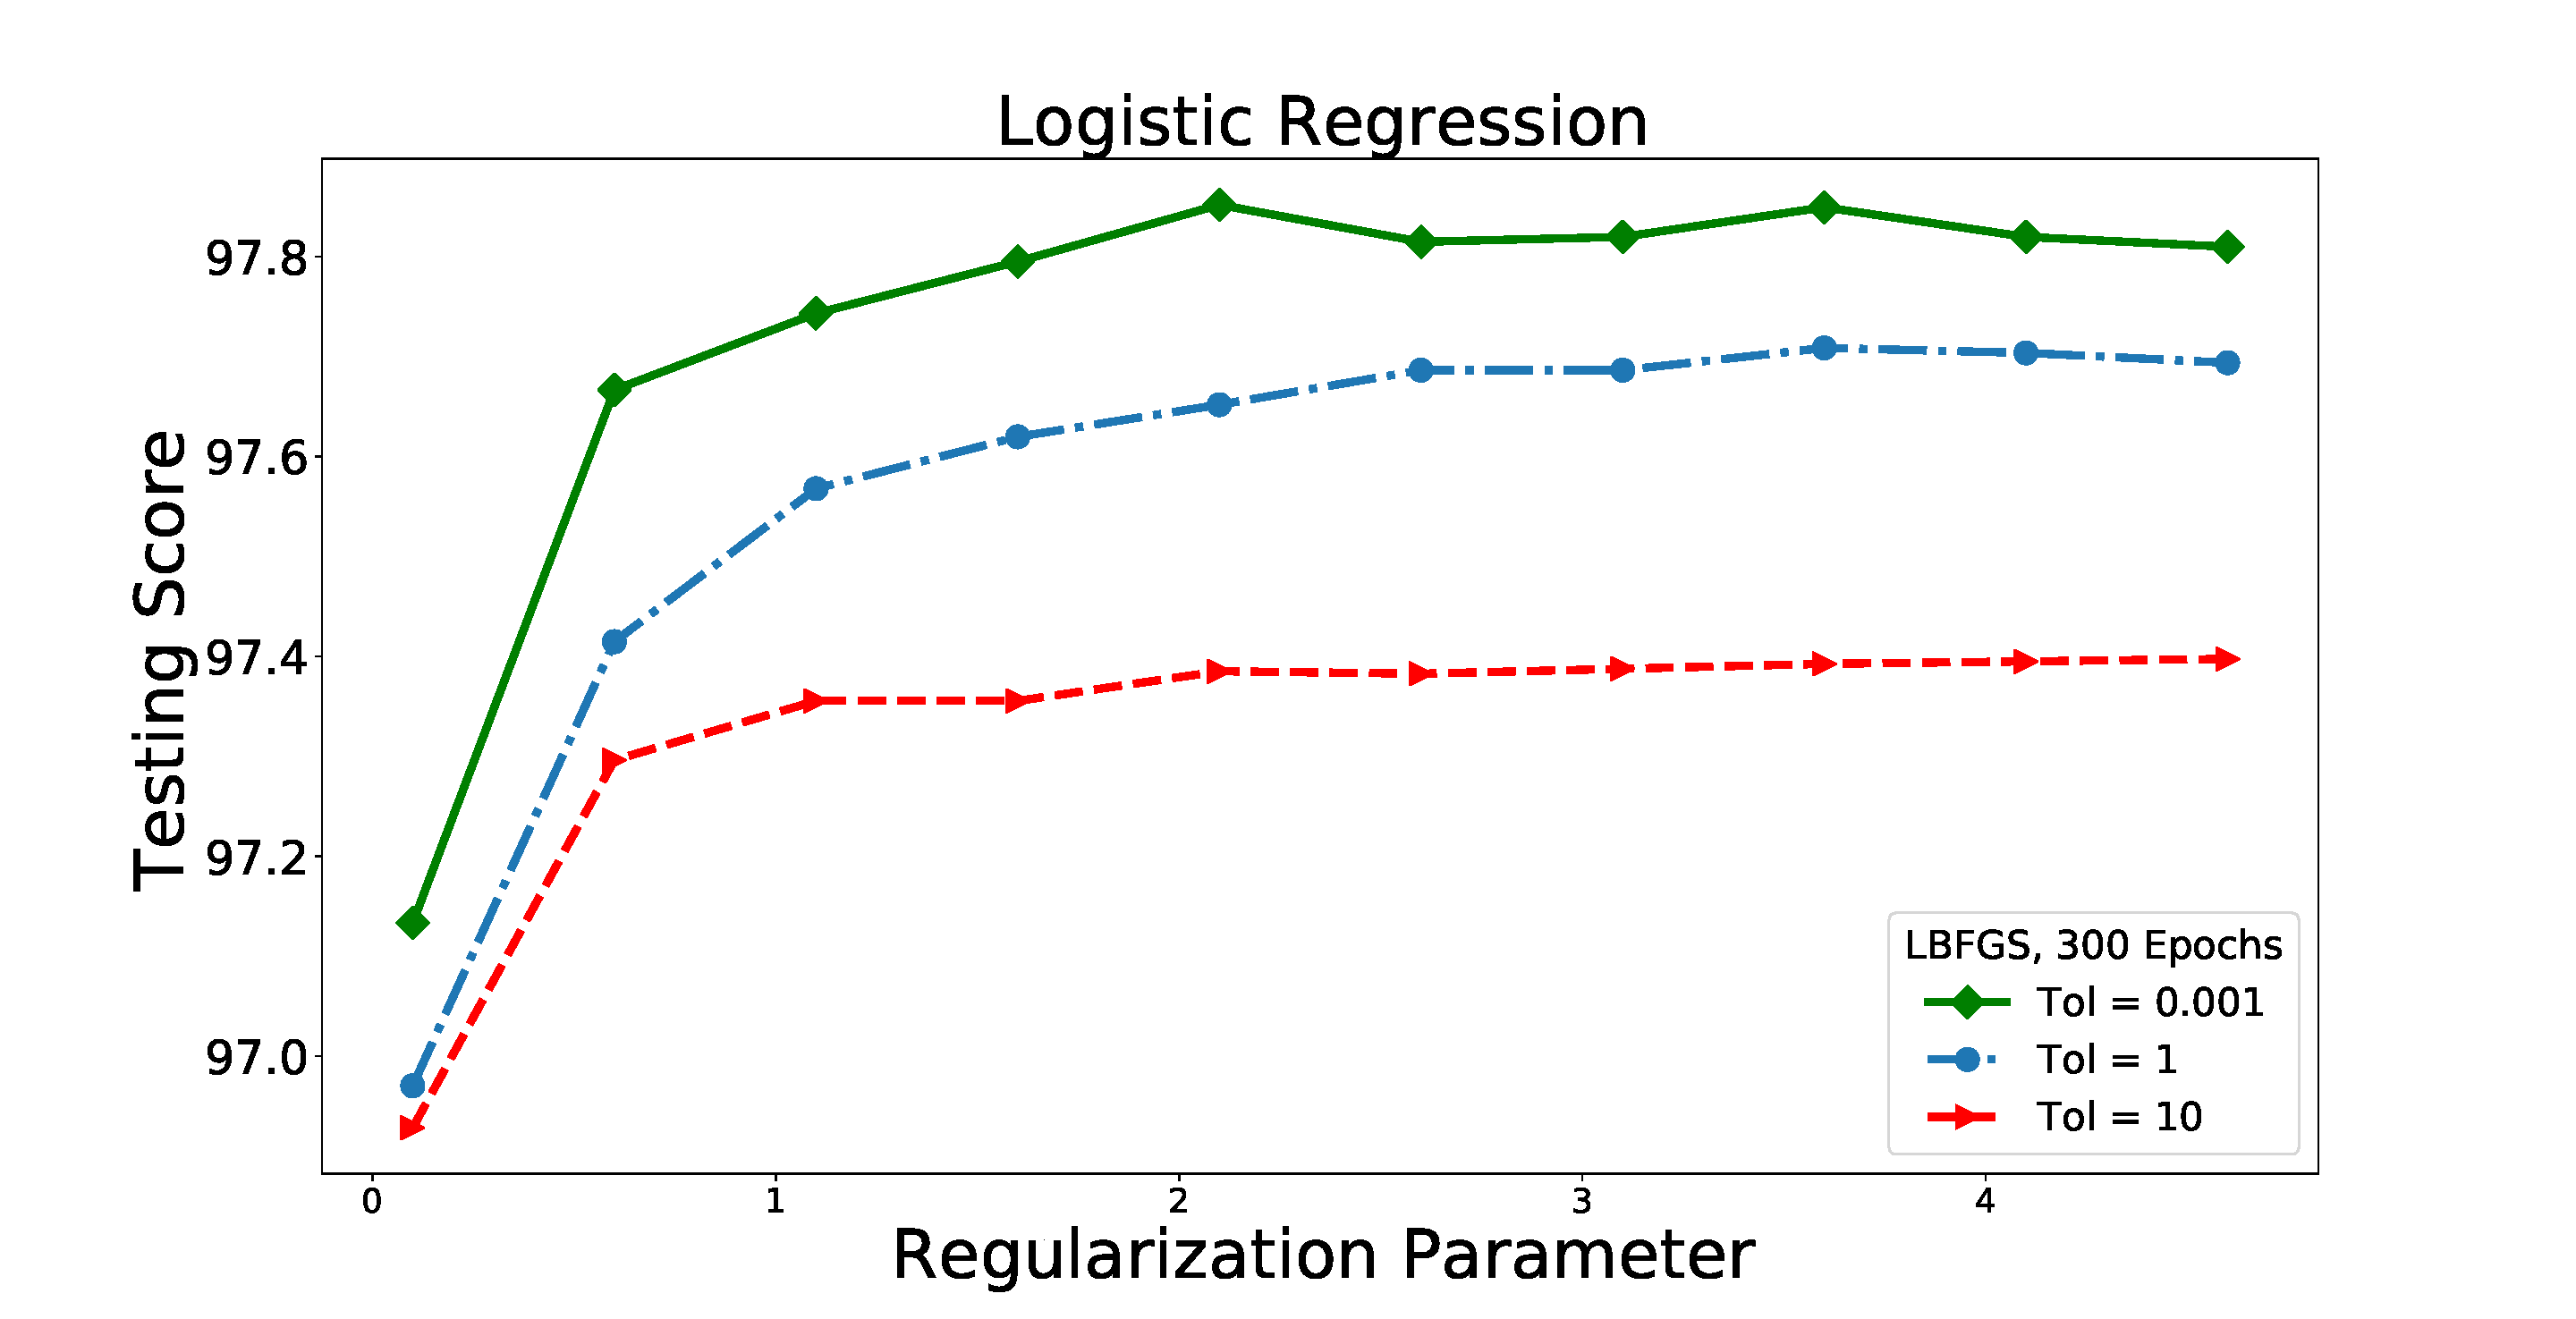
\includegraphics[width=\twopicsp\textwidth]{plots/lr_train_reg.pdf}
\caption{Dependence of LR accuracy on the regularization parameter}
%\dima{I think it's a wrong plot for regularization (it says tolerance in the plot title). 
%I'm not sure we need to plot accuracy vs tolerance or iterations.
%Also please add the algorithm names in the filenames.}}
\label{fig:LR_accuracy}
\end{figure}

Classification domains are presented in Figure \ref{fig:LR_domains}. As can be seen, when a Neural Network with no hidden layer is compared, the results are almost identical. \\

\begin{figure}[h]
%\centerin
\hspace*{-1.5cm}
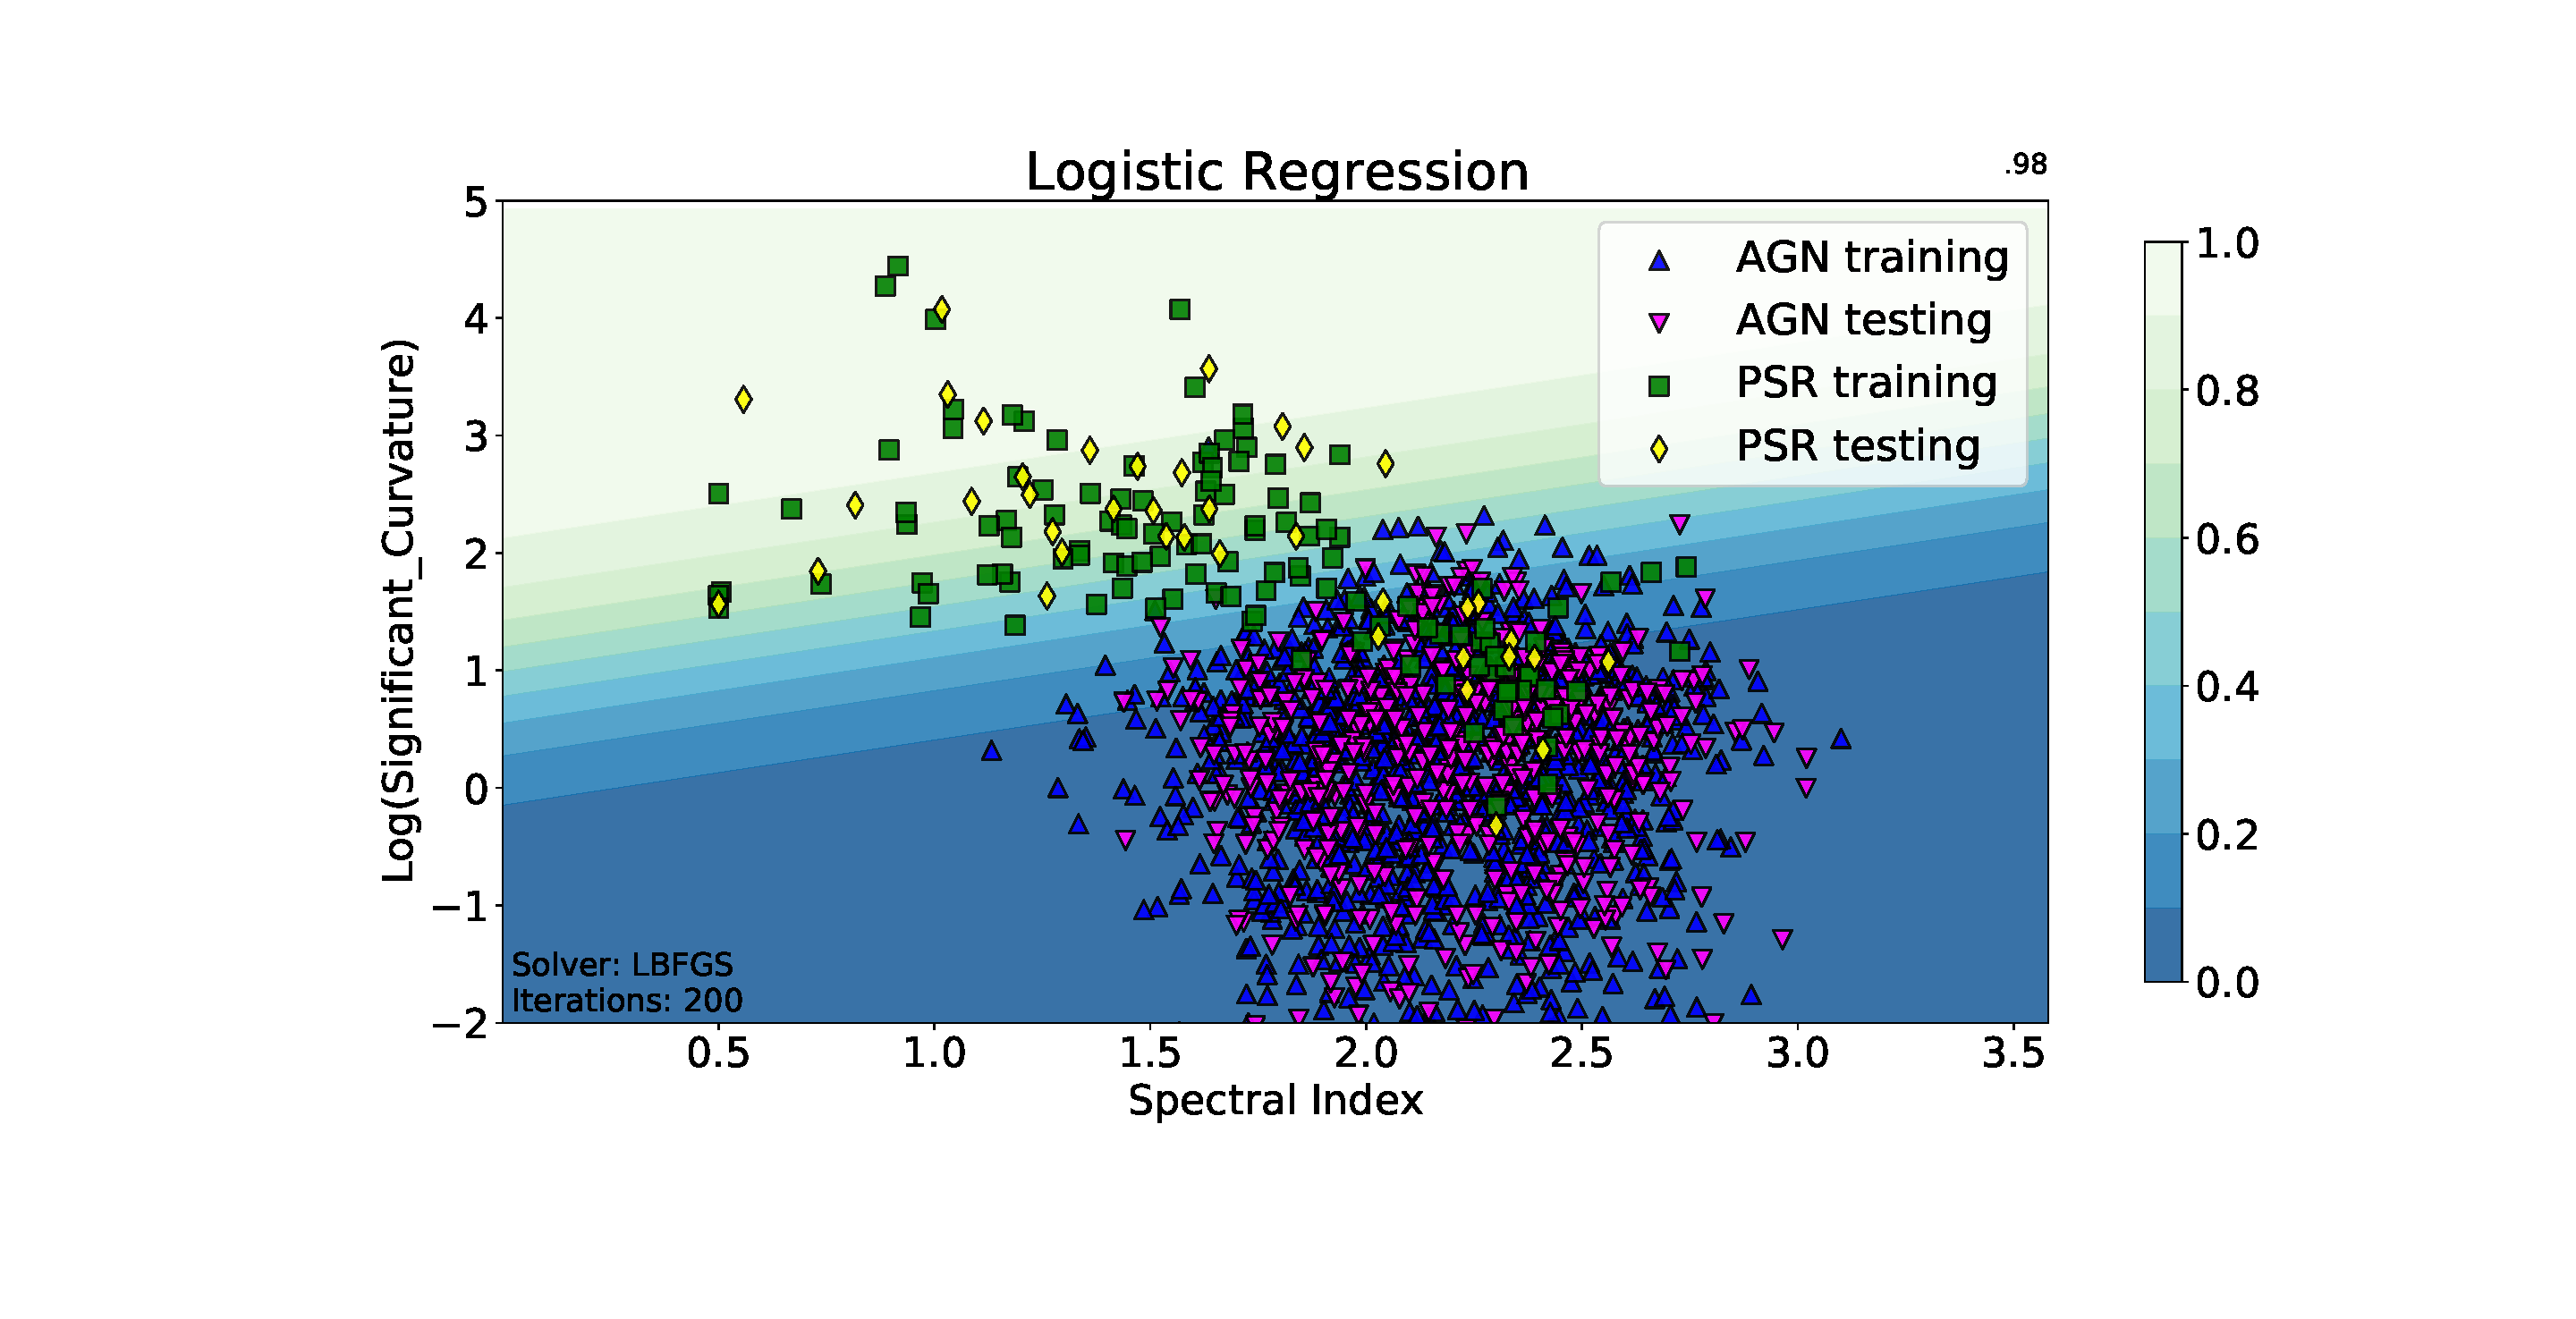
\includegraphics[width=0.6\textwidth]{plots/classification_domains/lr_200_lbfgs.pdf}
%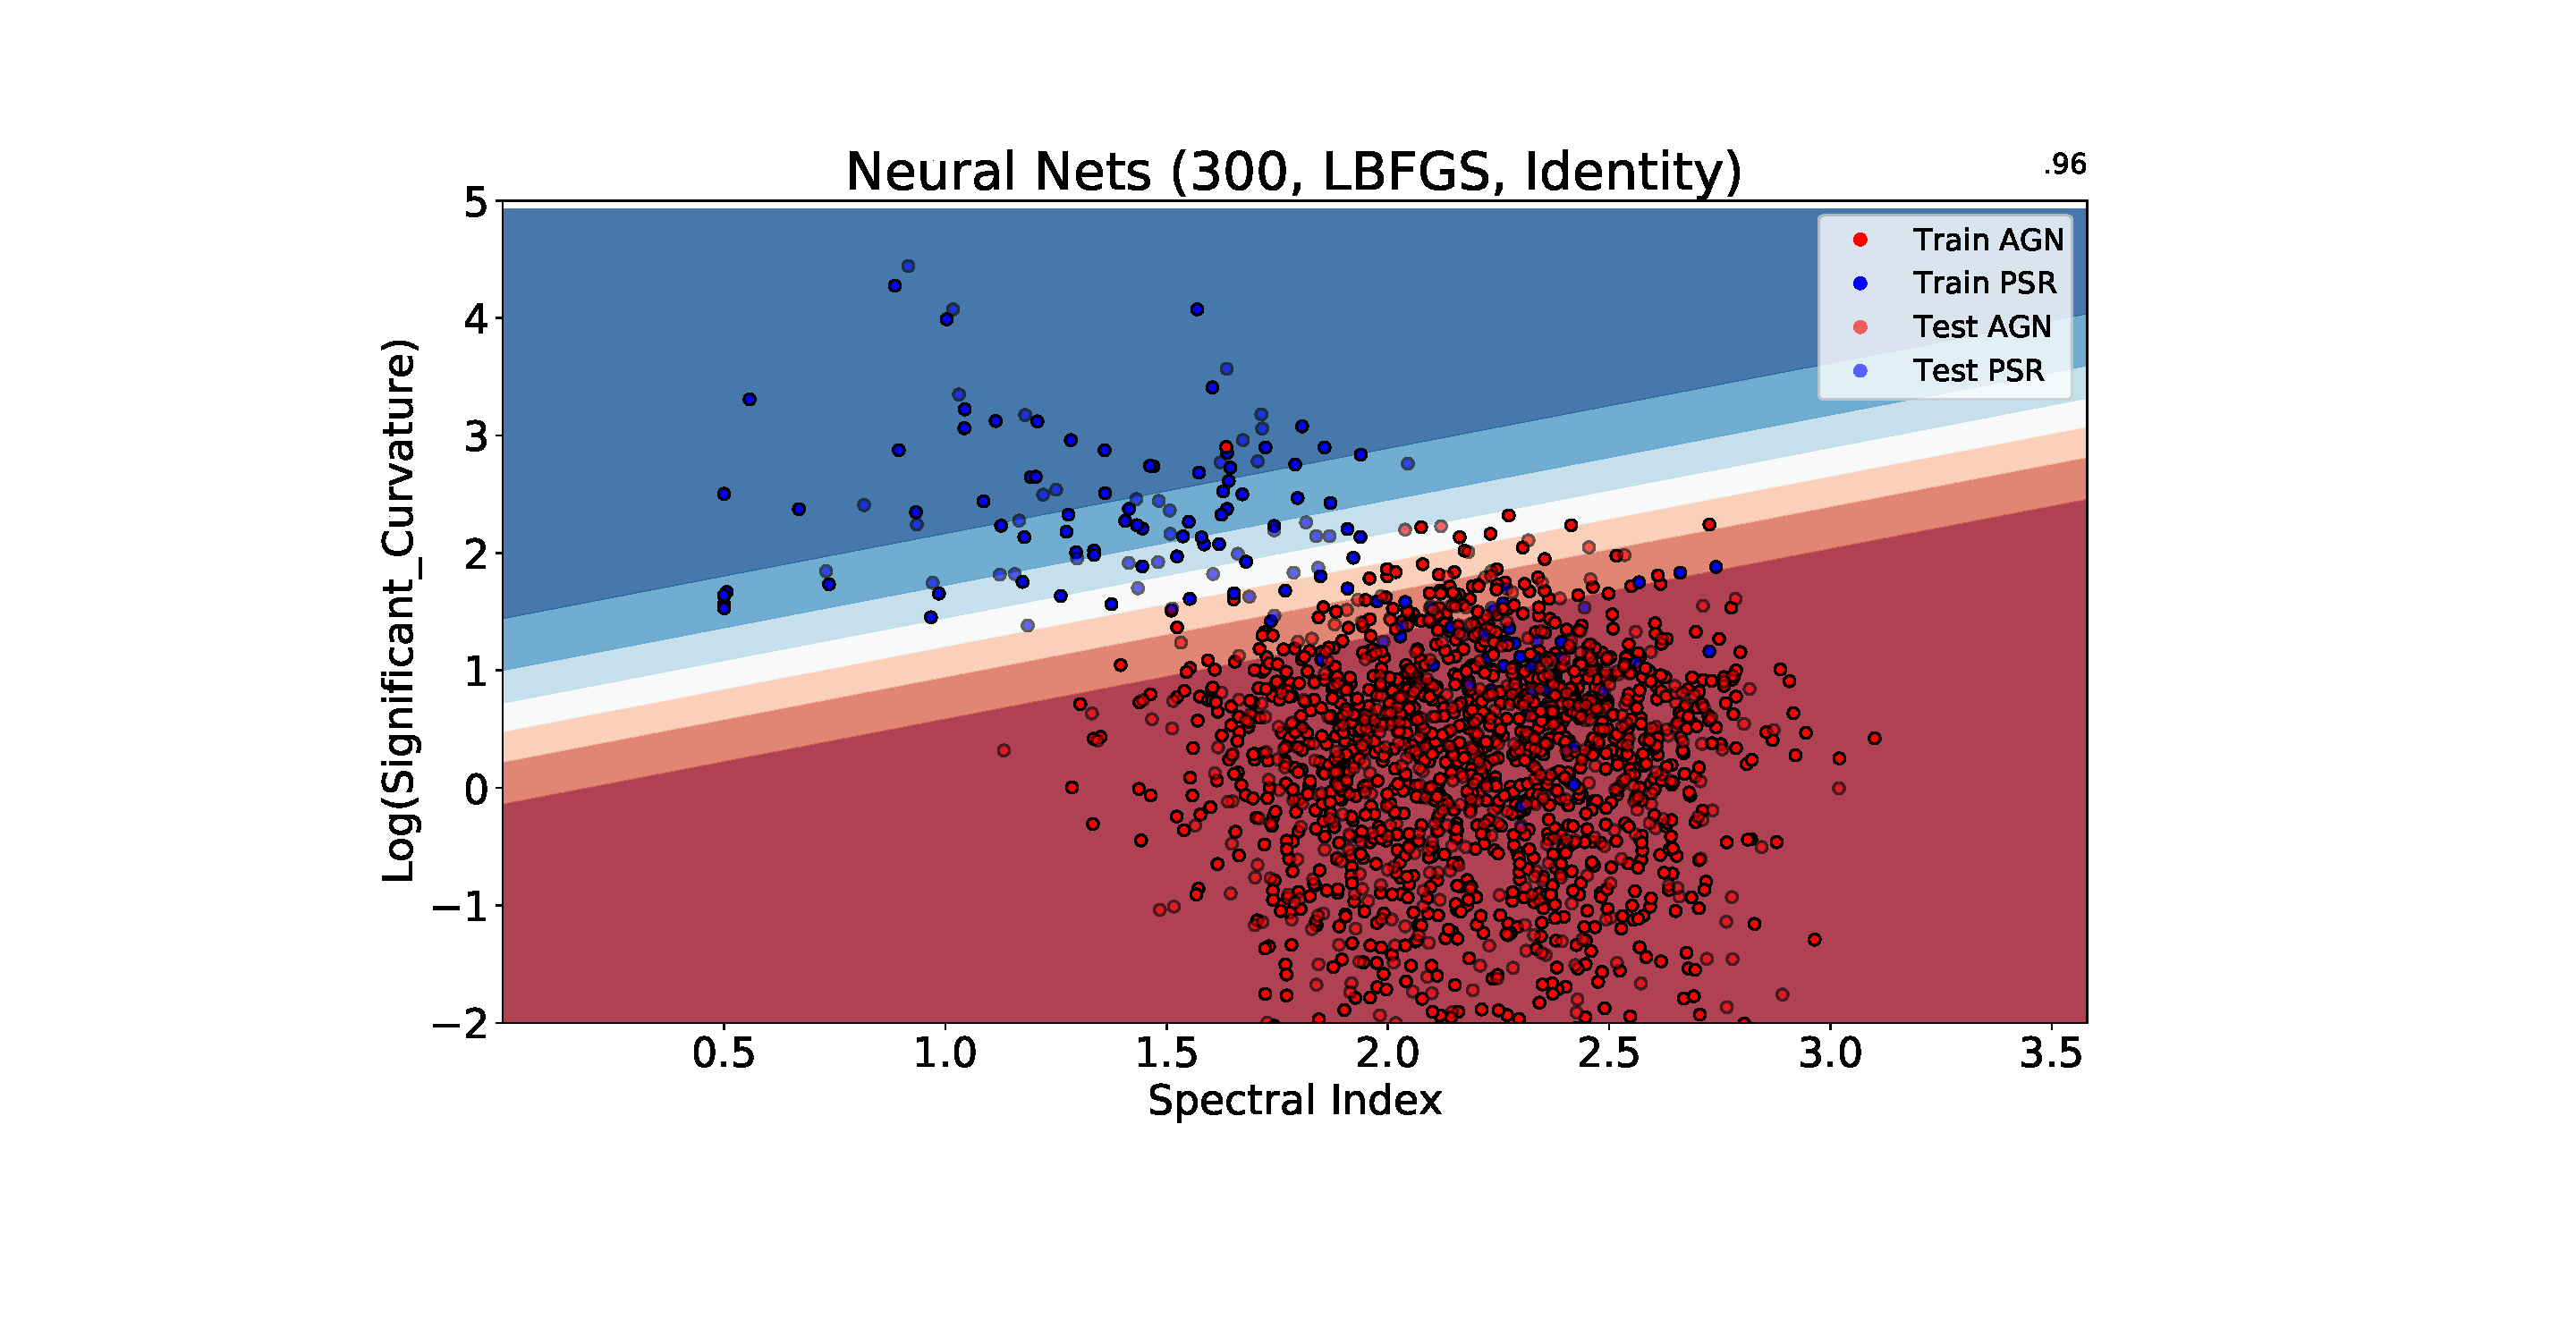
\includegraphics[width=\twopicsp\textwidth]{plots/classification_domains/NN_300_LBFGS_Identity.pdf}
\caption{Classification domains for Logistic Regression}
%\dima{There should be a set of parameters, which gives the same result as for the NN in Figure \ref{fig:NN_domains}.}}
\label{fig:LR_domains}
\end{figure}



\section{Probabilistic catalogs based on the 3FGL and 4FGL catalogs}
\lb{sec:prob_cats}

In this section we use the ML algorithms optimized in the previous section to construct probabilistic
classification of sources in the 3FGL and 4FGL catalogs.
%Having optimized our algorithms, we decided to test them on 3FGL data which was initially unassociated but then became associated in 4FGL. Furthermore, we tested the algorithms on 4FGL associated data, and also predicted for unassociated data.


\subsection{Probabilistic classification of sources in 3FGL and comparison with 4FGL}
\lb{sec:3FGLprediction1}


%In this section we perform probabilistic classification of sources in the 3FGL catalog.
We use the following four algorithms for the classification of sources: RF with 50 trees and maximal depth of 6, BDT with 100 trees and maximal depth of 2, NN with 11 neurons, LBFGS solver, and 300 epochs, and LR with LBFGS solver and 200 iterations. 
For training we use the pulsars and AGNs from the 3FGL catalog. In addition to original datasets, we perform oversampling of pulsars in order to balance the numbers of pulsars and AGNs.
As a result, we have 8 classification methods: 4 algorithms trained with and without oversampling.


\begin{table}[!h]
\hspace{-0.2cm}
\resizebox{0.47\textwidth}{!}{
    \tiny
  \centering
    \renewcommand{\tabcolsep}{0.4mm}
\renewcommand{\arraystretch}{1.6}

%\hspace{-3mm}
    \begin{tabular}{|c|c|c|c|c|c|c|}
    \hline
    Algorithm&Parameters &  Testing&Std. Dev.& Comparison with \\
    & & Accuracy & & 4FGL-DR2 Accuracy \\
    \hline
    RF & 50 trees, max depth 6  &97.37&0.60& 91.41  \\
    RF\_O &   &97.90&0.50& 90.28 \\
    \hline %\midrule   -> aakash do you mean this?
    BDT & 100 trees, max depth 2    &   97.65&0.54&90.64 \\
%    \hline %\midrule   -> aakash do you mean this?
%    BDT & 200 trees, max depth 2    &   95.8  \\
    BDT\_O &     &   97.79&0.51& 90.79 \\
    \hline
    NN & 300 epochs, 11 neurons, LBFGS & 97.29&0.97& 89.32\\
    NN\_O &  & 94.31&5.13& 85.99\\
    \hline
    LR & 200 iterations, LBFGS solver & 97.63&0.54& 89.97 \\
    LR\_O &  &93.68&0.99& 85.55\\
    \hline
     
    \end{tabular}}
    \vspace{2mm}
    \caption{Testing accuracy of the 4 selected algorithms for classification of 3FGL sources and comparison with associations in the 4FGL-DR2 catalog. 
    ``\_O'' denotes training with oversampling.}
    \label{tab:selected_algs}
\end{table}



\begin{figure}[h]
\centering
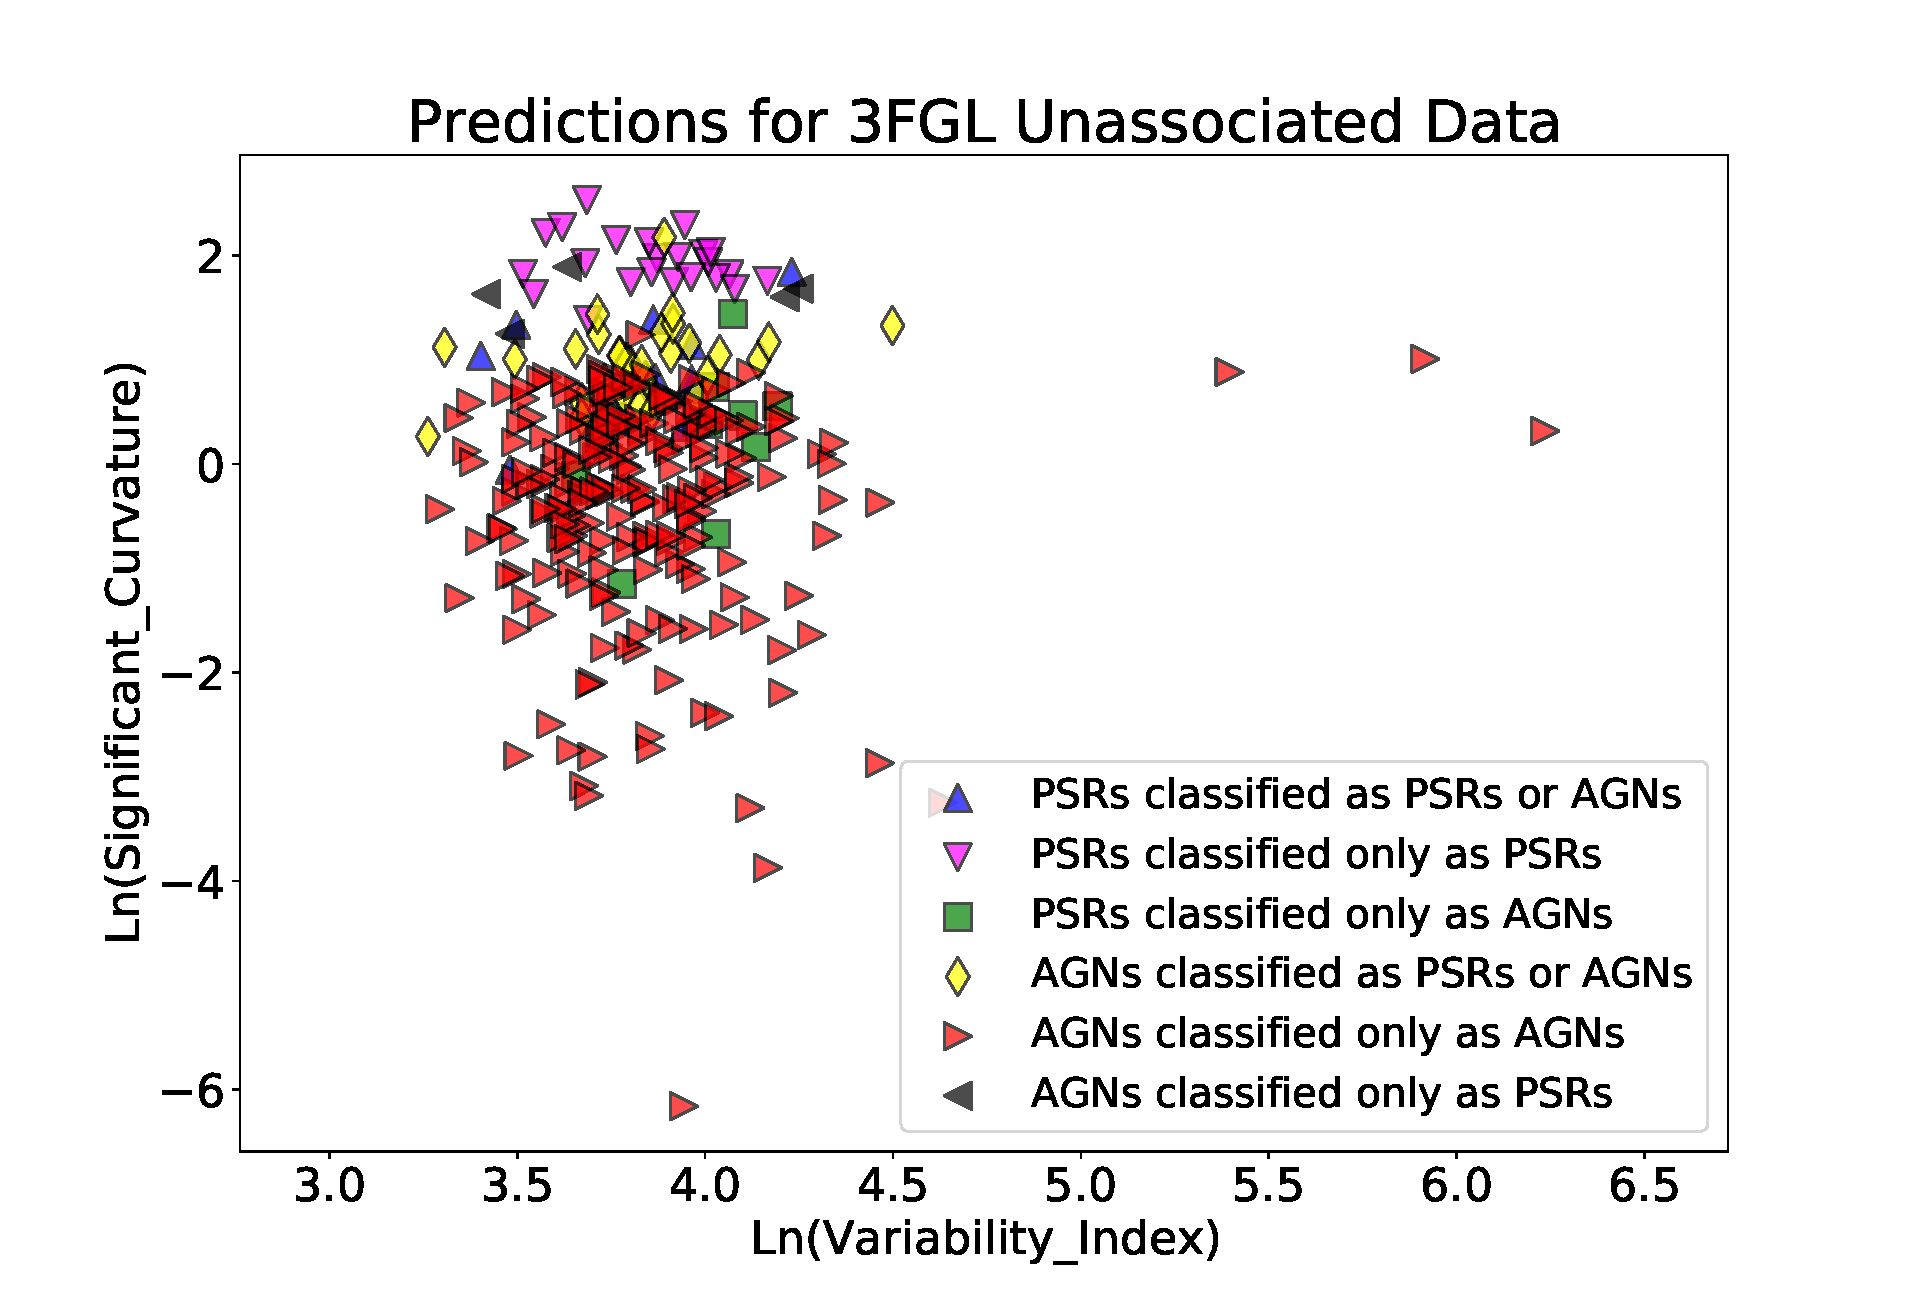
\includegraphics[width=0.48\textwidth]{plots/plot_final_DR2.pdf}
%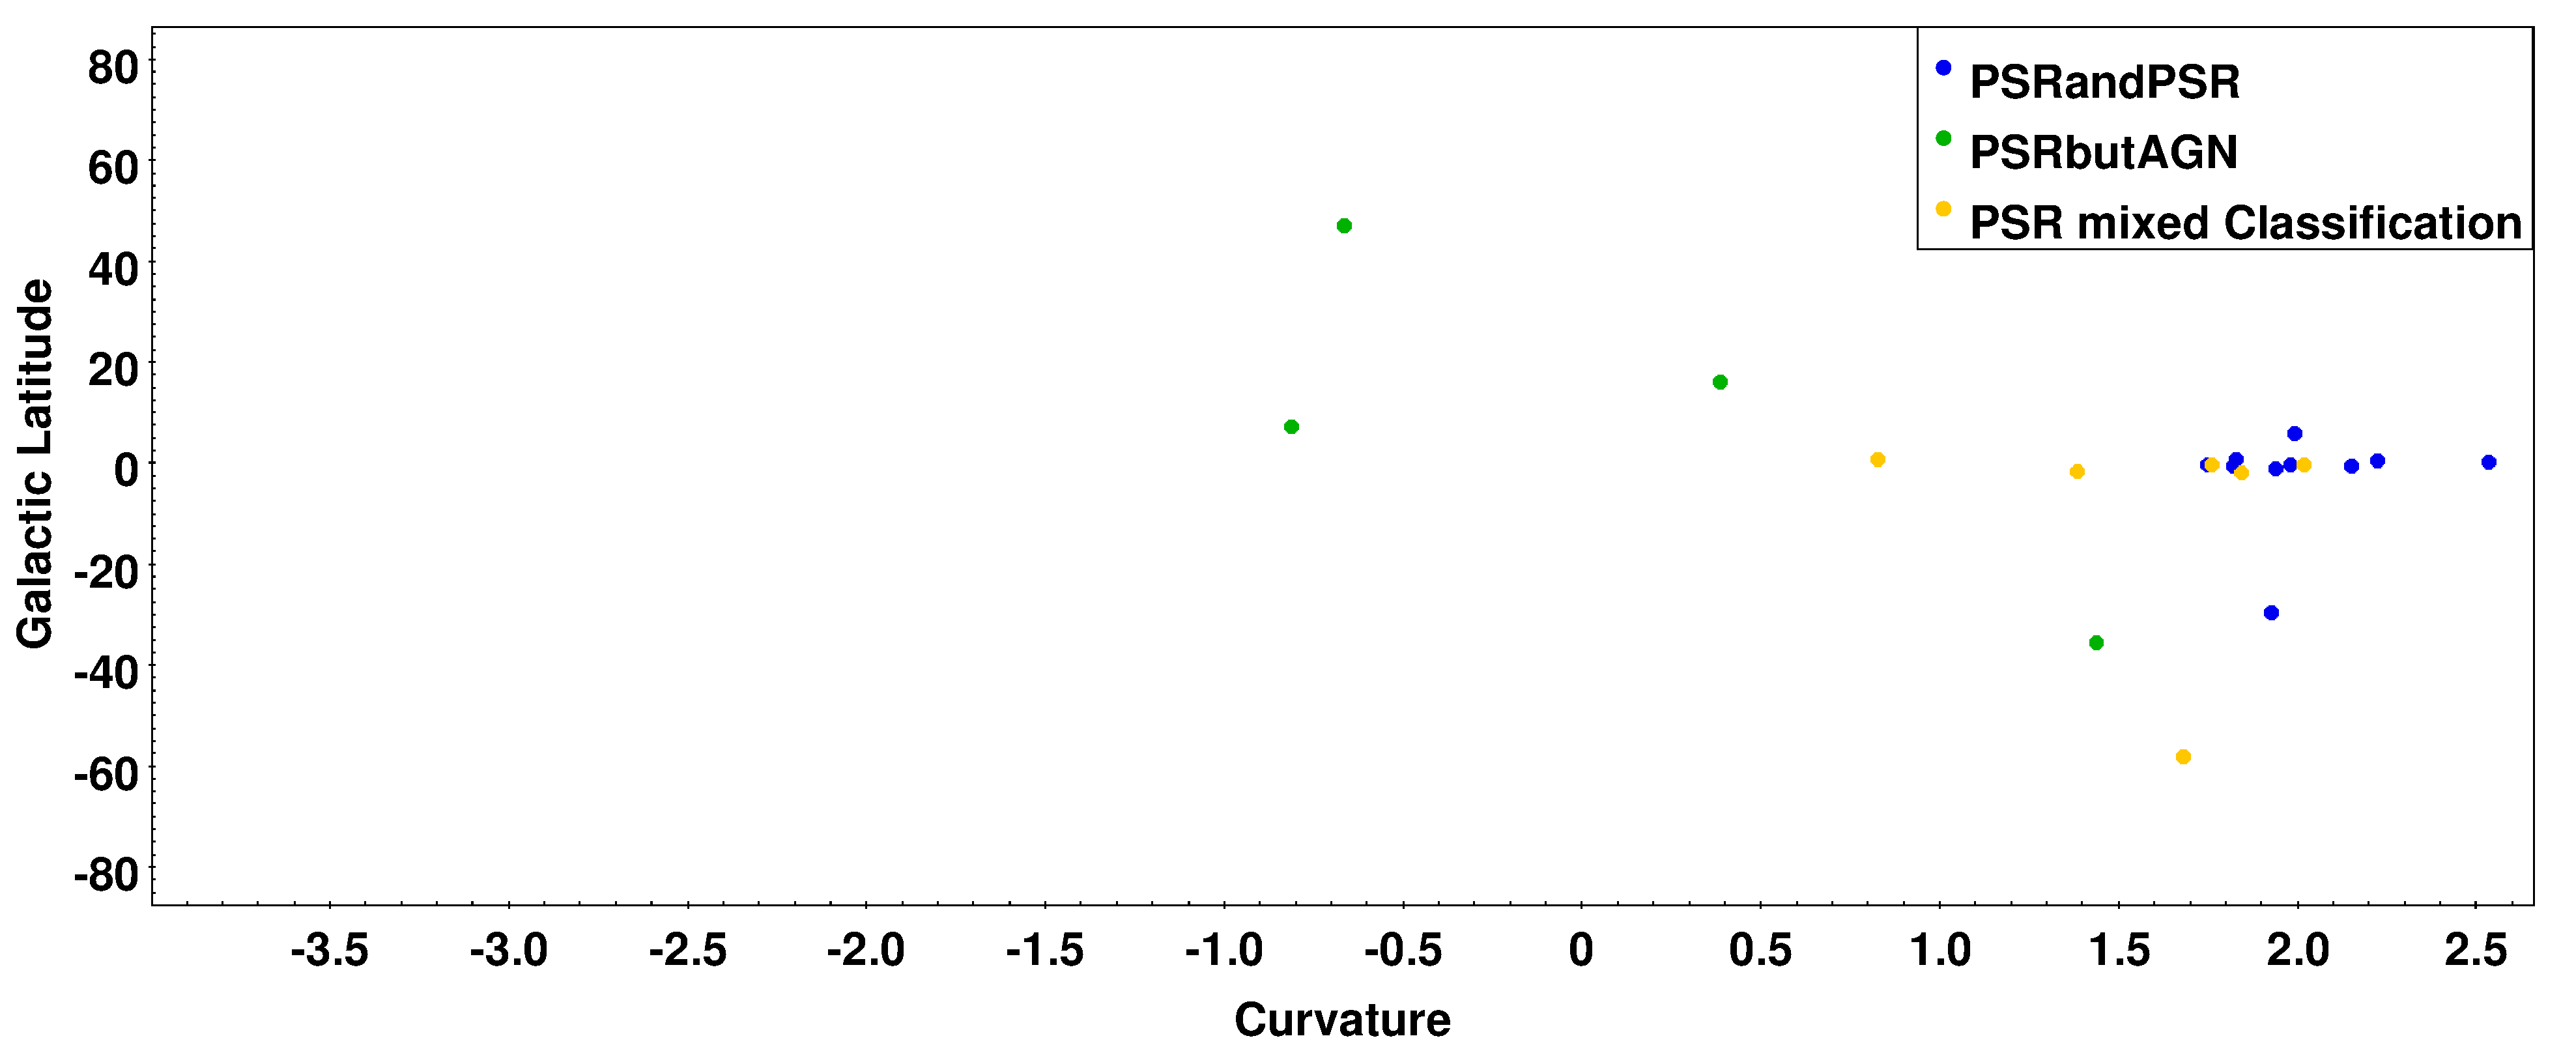
\includegraphics[width=\twopicsp\textwidth]{plots/PSR3.pdf}
\caption{Comparison of class prediction for unassociated 3FGL sources with classes in 4FGL-DR2. 
For more details see Section \ref{sec:3FGLprediction1}.}
%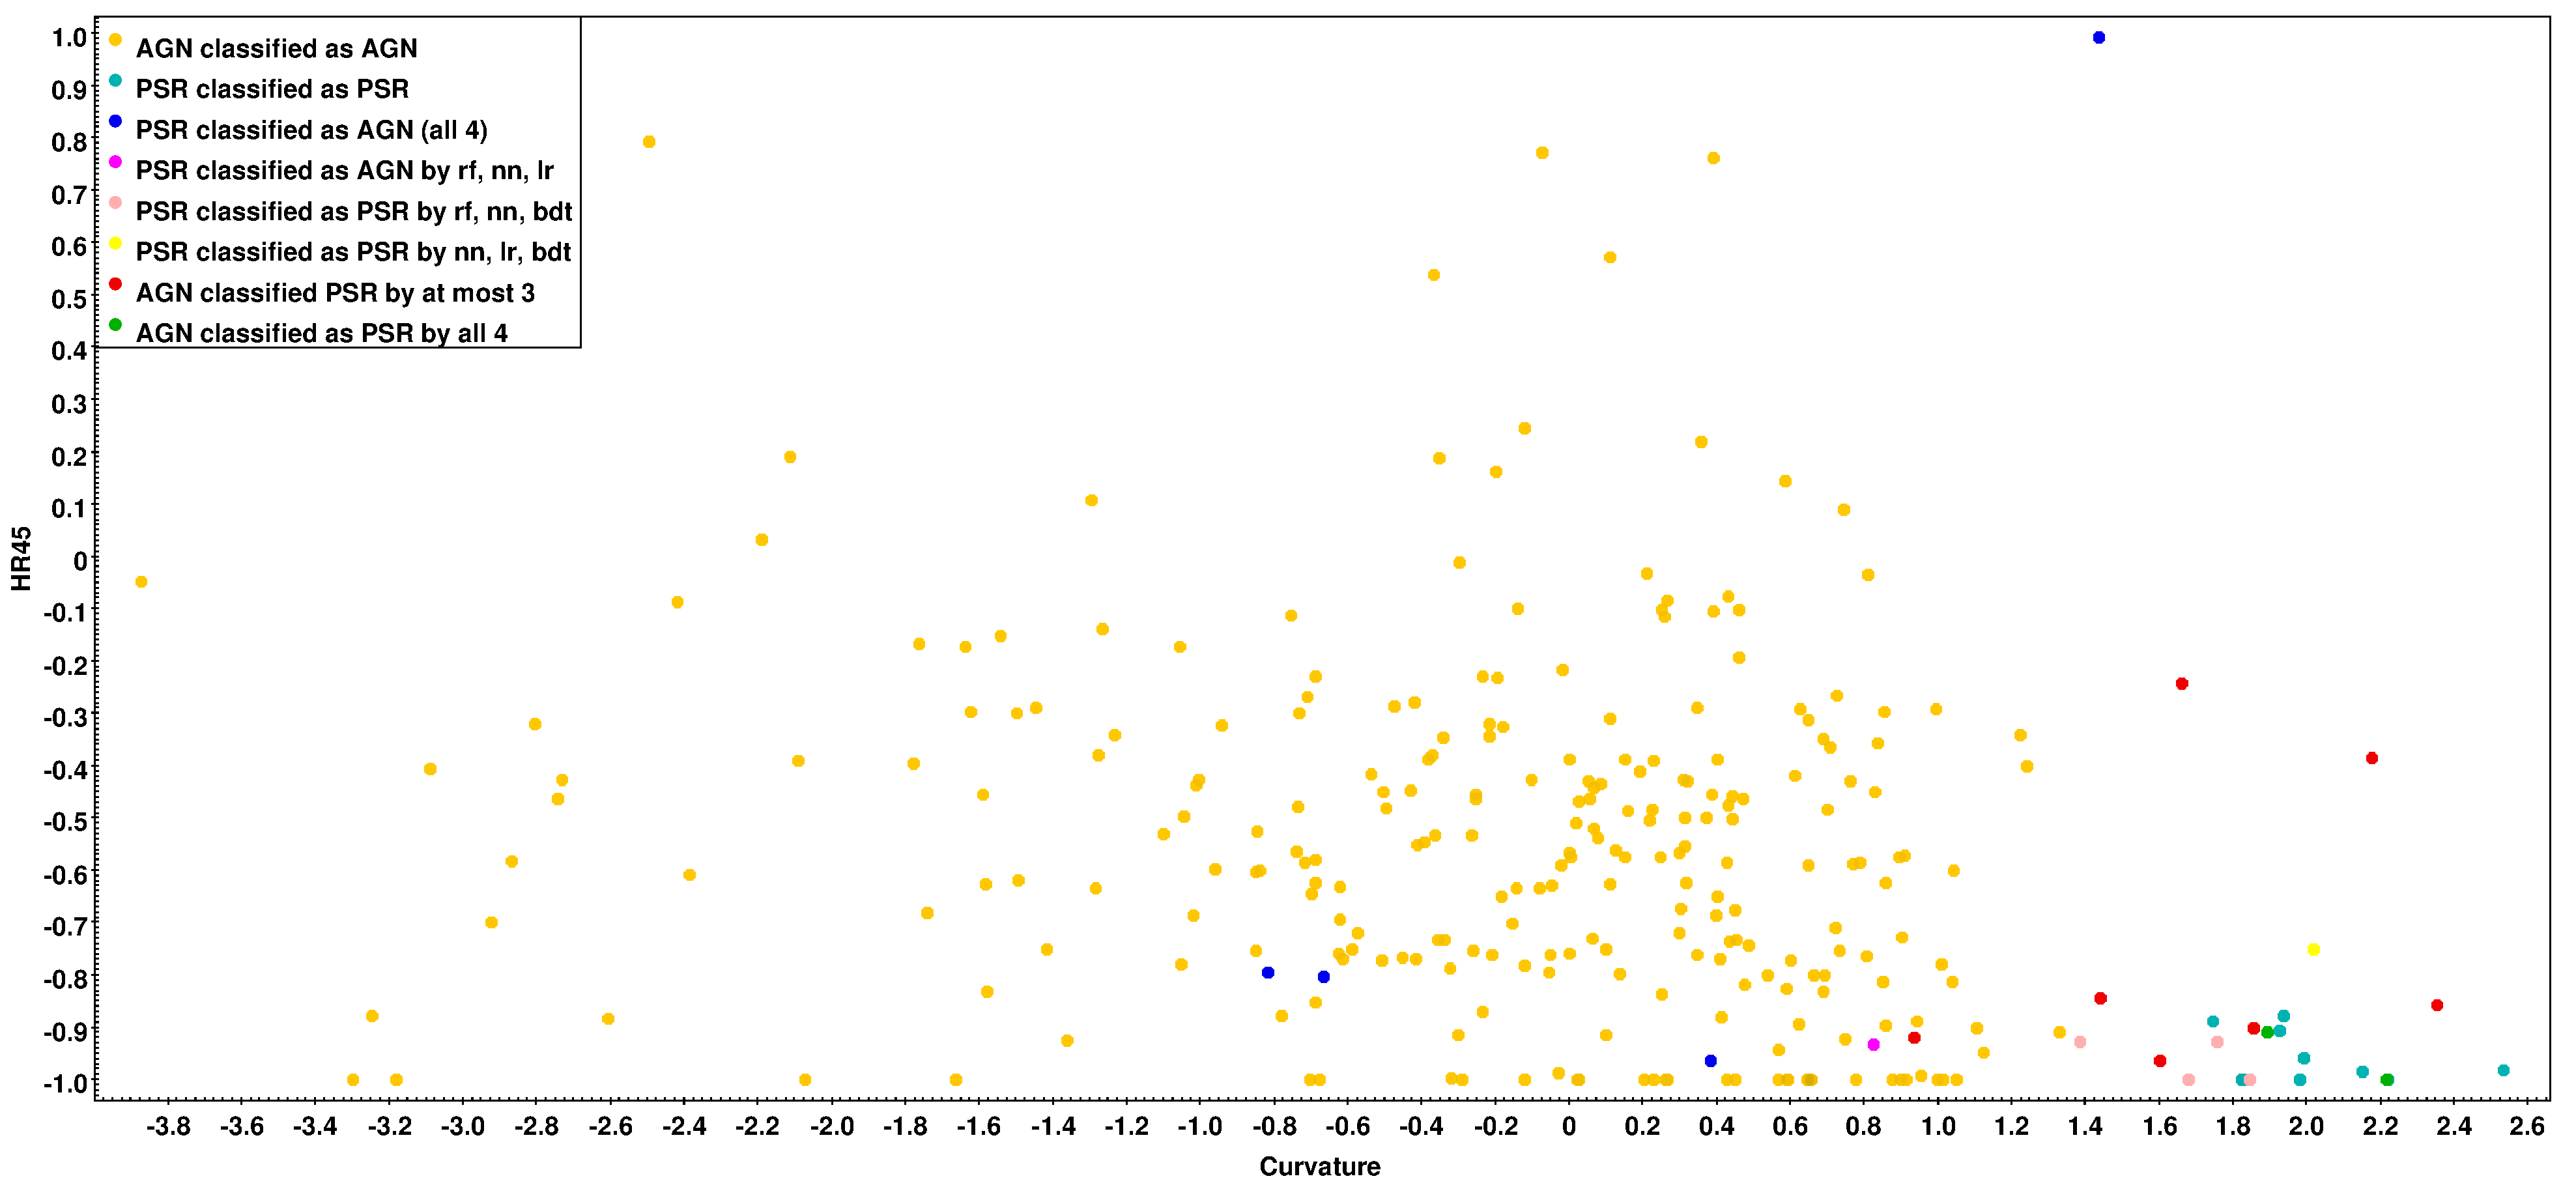
\includegraphics[width=\twopicsp\textwidth]{plots/final_catalog.pdf}
\label{fig:3FGL_vs_4FGL_classes}
\end{figure}

The selected algorithms are summarized in Table \ref{tab:selected_algs}, where oversampling is shown by ``\_O''.
``Average testing accuracy'' is computed by taking 1000 times 70\% - 30\% split into training and testing samples and averaging over the 
accuracies computed for the testing samples.
In addition, we look at sources, which are unassociated in 3FGL but have either pulsar or AGN association in 4FGL-DR2: there are 302 such sources.
The accuracy of our prediction for the four selected algorithms with and without oversampling, taking the 4FGL-DR2 classes as the true values, is reported in the column ``Comparison with 4FGL Accuracy''.
The correct classifications and misclassifications for the 302 sources with PSR or AGN associations in 4FGL-DR2 are also presented in Figure \ref{fig:3FGL_vs_4FGL_classes}.
The class at the beginning of the label name corresponds to the association in the 4FGL-DR2, while the second half of the labels corresponds to classification of unassociated sources in 3FGL. For example, ``PSRs classified only as PSRs'' shows sources which have PSR association in 4FGL-DR2 and all eight methods classified the corresponding unassociated sources in 3FGL as a pulsar. ``PSRs classified as either PSRs or AGNs'' labels sources with PSR associations in 4FGL-DR2 but the corresponding unassociated sources in 3FGL have both PSR and AGN classifications by different ML methods.
The unassociated sources are classified as PSRs or AGNs if the corresponding probability is larger than 0.5.
We notice that misclassified or partially misclassified sources in Figure \ref{fig:3FGL_vs_4FGL_classes} typically happen on the boundary between the two classes or even inside the opposite class.
Many of these sources also have flags in the 3FGL catalog, such as a potential problem with the background diffuse emission model in the location of the source, which can lead to a poor reconstruction of the source spectrum and, consequently, misclassification of the source.


As a result of the classification with the eight ML methods,
we created a probabilistic catalog based on the 3FGL sources without missing values.%
\footnote{There are thirteen sources with missing values in the 3FGL catalog (2 unassociated, 5 AGNs, 1 pulsar, and 5 ``other'' sources), 
which we save in a separate file ``3FGL\_sources\_with\_missing\_values.csv'' for reference. In particulat all of these sources have a value in significant curvature of 0.
%\dima{Which features are missing for these sources, could we still classify them?}
}
We train on 70\% of the sources associated with pulsars or AGNs and save the probability values for testing sources, for sources which are not classified as pulsars or AGNs, and for unassociated sources.
We repeat the splitting and training 1000 times and report the sample average and standard deviation of the classification probabilities,
i.e., we average over 1000 values for unassociated sources and sources not classified as AGNs or pulsars, 
while the average for AGNs and pulsar is over the number of times the sources appear in the testing sample, which is 300 on average.
%Like in the case of associated sources, where we split the data 1000 times, we also do a 1000 runs for the unassociated case. This allows us to calculate individual probabilities and their standard deviations for all sources.
%\dima{Classification of associated sources is done by averaging over testing-training samples splits.
%Do we also do averaging for unassociated sources?}
We have also subselected the 302 unassociated 3FGL sources, which have PSR or AGN associations in 4FGL-DR2,
and saved them for convenience of comparison as a separate file.

In the probabilistic catalogs we add columns with corresponding probabilities for each algorithm and each class,
i.e., provided that there are 8 methods (including oversampling) and 2 classes, we add 16 columns: 8 for unweighted and 8 for oversampled training data. The columns with '\_O' represent the oversampled probabilities. We also add 16 columns for standard deviations of probabilities. Although class probabilities and standard deviation for each algorithm are not independent (probabilities add up to 1 and standard deviations are equal for AGN and PSR classes), we keep the corresponding columns in view of the generalizations to multi-class classification (e.g., 3-class classification in Section \ref{sec:3class}).
%Although the class probabilities for each algorithms should add up to one for every source, we still keep the columns for all classes for convenience.
Table \ref{tab:prob_cat} shows an example of the probabilistic catalog for a few unassociated 3FGL sources.
Notice that the first source is classified as a pulsar by BDT and as an AGN by RF, LR, and NN algorithms,
it is an example of a source with mixed classification.
%i.e., it has a label ``classified either as PSRs or AGNs'' in Figure \ref{fig:3FGL_vs_4FGL_classes}. - is it associated in 4FGL?
%The second and third sources are classified as AGNs by all four algorithms, i.e., they will have a label ``classified only as AGNs'',
%while the last source is classified as a pulsar by all four algorithms, i.e., it will have a label ``classified only as PSRs''.
Out of 1008 unassociated sources in 3FGL, 111 are classified as pulsars by all eight methods, 597 are classified as AGNs, and 300 have mixed classifications.
Out of 111 sources classified as pulsars, 6 sources have counterparts in Parkes survey \citep{Camilo2015} within 2 arc minutes (see Table \ref{tab:parkes}).

We summarize the results of classification of unassociated sources in Table \ref{tab:prediction_2and3class} in the ``2-class'' row.
The ``AGNs'' column shows the number of unassociated sources where all eight methods from Table \ref{tab:selected_algs} 
give the probability for a source to be an AGN above 50\%.
Similarly the ``Pulsars'' column shows the number of unassociated sources where all algorithms predict the source to be more likely a pulsar.
The ``Mixed'' column shows the number of sources with mixed classification, i.e., some algorithms predict that the source is more likely an AGN while the other algorithms predict that it is more likely a pulsar.
We also add the ``OTHER'' column in order to compare the results with the 3-class classification later in this Section.
Since there is no ``OTHER'' class in the 2-class classification, the corresponding entry is empty.
In the ``2-class corr'' row we show a possible correction of the number of pulsars and AGNs due to presence of other sources.
Here we assume that the fraction of AGN-like and pulsar-like sources among the other sources is the same for associated and for unassociated sources.
In particular, if we denote by $N_{\rm AGN}$ the number of unassociated sources with AGN-like probabilistic classification,
by $N_{\rm AGN}^{\rm ass\,OTHER}$ the number of sources with AGN-like classification among associated OTHER sources,
by $N_{\rm ass}$ ($N_{\rm unass}$) the total number of associated (unassociated) sources, then
the number of AGN-like sources among the unassociated ones corrected for the presence of OTHER sources can be estimated as

\be
\lb{eq:other_correction}
N_{\rm AGN}^{\rm corr} = N_{\rm AGN} - N_{\rm AGN}^{\rm ass\,OTHER} \,\frac{N_{\rm unass}}{N_{\rm ass}}.
\ee
Analogous corrections are applied for the number of unassociated sources with PSR and with mixed classifications.
If we denote by $N^{\rm ass\,OTHER}$ the total number of associated other sources, then the estimated number of 
OTHER sources among unassociated ones is
\be
\lb{eq:2class_other}
N^{\rm unass}_{\rm OTHER} = N^{\rm ass\,OTHER} \,\frac{N_{\rm unass}}{N_{\rm ass}}.
\ee
We show this estimate in the OTHER column in the ``2-class corr'' row.
We note that since 
$N_{\rm AGN}^{\rm ass\,OTHER} + N_{\rm PSR}^{\rm ass\,OTHER} + N_{\rm MIXED}^{\rm ass\,OTHER} = N^{\rm ass\,OTHER}$,
this estimate is consistent with corrections in Equation (\ref{eq:other_correction}) for sources classified as AGNs, pulsars, or with mixed classification.


\pgfplotstableread[col sep=comma]{tables/3FGL_unassoc_vs_4FGL_assoc.csv}\loadedtable
\begin{table}
\pgfplotstabletypeset[columns={Source_Name_3FGL,AGN_BDT,AGN_RF,AGN_LR,AGN_NN},
column type=l,
string type,
every head row/.style={before row={\toprule & \multicolumn{4}{c}{AGN Probability} \\},after row=\midrule,},
every last row/.style={after row=\midrule}, %\vdots },
columns/Source_Name_3FGL/.style={column name=Source\_Name\_3FGL},
columns/AGN_BDT/.style={column name=BDT,numeric type,fixed,precision=3},
columns/AGN_NN/.style={column name=NN,numeric type,fixed,precision=3},
columns/AGN_RF/.style={column name=RF,numeric type,fixed,precision=3},
columns/AGN_LR/.style={column name=LR,numeric type,fixed,precision=3},
skip rows between index={4}{302}
]\loadedtable
\caption{\label{tab:prob_cat}
Example of the AGN classification probabilities for a few unassociated sources in the 3FGL catalog \citep{2015ApJS..218...23A}. We have ommited the oversampled probability columns here.}
\end{table}




\pgfplotstableread[col sep=comma]{tables/3fgl_unassoc_predictions_matches_with_Parkes(2015)_1.csv}\loadedtable
\begin{table}
\pgfplotstabletypeset[columns={Source_Name_3FGL,GLON,GLAT,Separation},
column type=l,
string type,
every head row/.style={before row={\toprule},after row=\midrule,},
every last row/.style={after row=\midrule },
columns/Source_Name_3FGL/.style={column name=Source\_Name\_3FGL},
columns/GLON/.style={column name=GLON,numeric type,fixed,precision=1},
columns/GLAT/.style={column name=GLAT,numeric type,fixed,precision=1},
columns/Separation/.style={column name=Sep (arksec),numeric type,fixed,precision=1}
]\loadedtable
\caption{\label{tab:parkes}
Connection of unassociated 3FGL sources classified as pulsars with Parkes pulsars \citep{Camilo2015}.}
\end{table}




\subsection{Probabilistic classification of sources in the 4FGL-DR2 catalog}
\lb{sec:4FGLprediction}

In this section we construct a probabilistic classification of sources in the 4FGL-DR2 catalog. The 4FGL-DR2 catalog \citep{2020arXiv200511208B} 
is based on 10 years of \Fermi-LAT data \citep[compared to 8 years of data in the 4FGL catalog,][]{2020ApJS..247...33A}.
It contains 5788 sources, which is 723 sources more than in the 4FGL catalog (all sources in 4FGL are kept in 4FGL-DR2 even if they fall
below the detection threshold with 10 years of data). 
3770 sources in 4FGL-DR2 have either an  AGN or a PSR classification, 
1658 sources are unassociated (we only look at CLASS1 column in the catalog), and the rest 346 sources are other sources with classification like PWN, SNR, etc.
There are 14 sources in 4FGL-DR2 with missing values: four AGNs, one PWN (Crab), and nine unassociated sources.
As in the previous section, we use for training and testing sources associated with either AGNs or pulsars,
which have no missing values used for classification.
%\footnote{In the 4FGL catalog there is only one source with missing values: 4FGL J0534.5+2201i associated with the Crab pulsar wind nebula.}
We then calculate the classification probabilities of AGN and PSR classes for both the associated and the unassociated sources.
The 4FGL catalog has higher number of features, especially due to the difference in modeling of the spectra compared with the 3FGL catalog. 
We selected 28 of these features and looked for correlations among them. If any feature was correlated or anti-correlated with a Pearson index of $\pm$0.75 or higher with another feature, then only one of these features was kept. 
%The correlation matrix is shown in Figure \ref{fig:corr_mat}.
The resulting 10 features are:
GLON, GLAT, ln(Pivot\_Energy), ln(Energy\_Flux100), ln(Unc\_Energy\_Flux100), LP\_Index, Unc\_LP\_Index, LP\_beta, LP\_SigCurv, ln(Variability\_Index).
In addition similar to the classification of the 3FGL sources, we add 6 hardness ratios to the list of features:
hr12, hr23, hr34, hr45, hr56, hr67 (in the 4FGL-DR2 catalog there are two more energy bins compared to the 3FGL catalog).
Thus, in total we use 16 features for classification of 4FGL-DR2 sources.
%Some of these features are direct counterparts to the features which we used in the 3FGL catalog, e.g., GLAT, LP\_Index (instead of 500MeV\_Index), LP\_SigCurv (instead of ln(Signif\_Curve)), ln(Variability\_Index), hardness ratios.

\begin{comment}
\begin{figure*}[h]
\centering
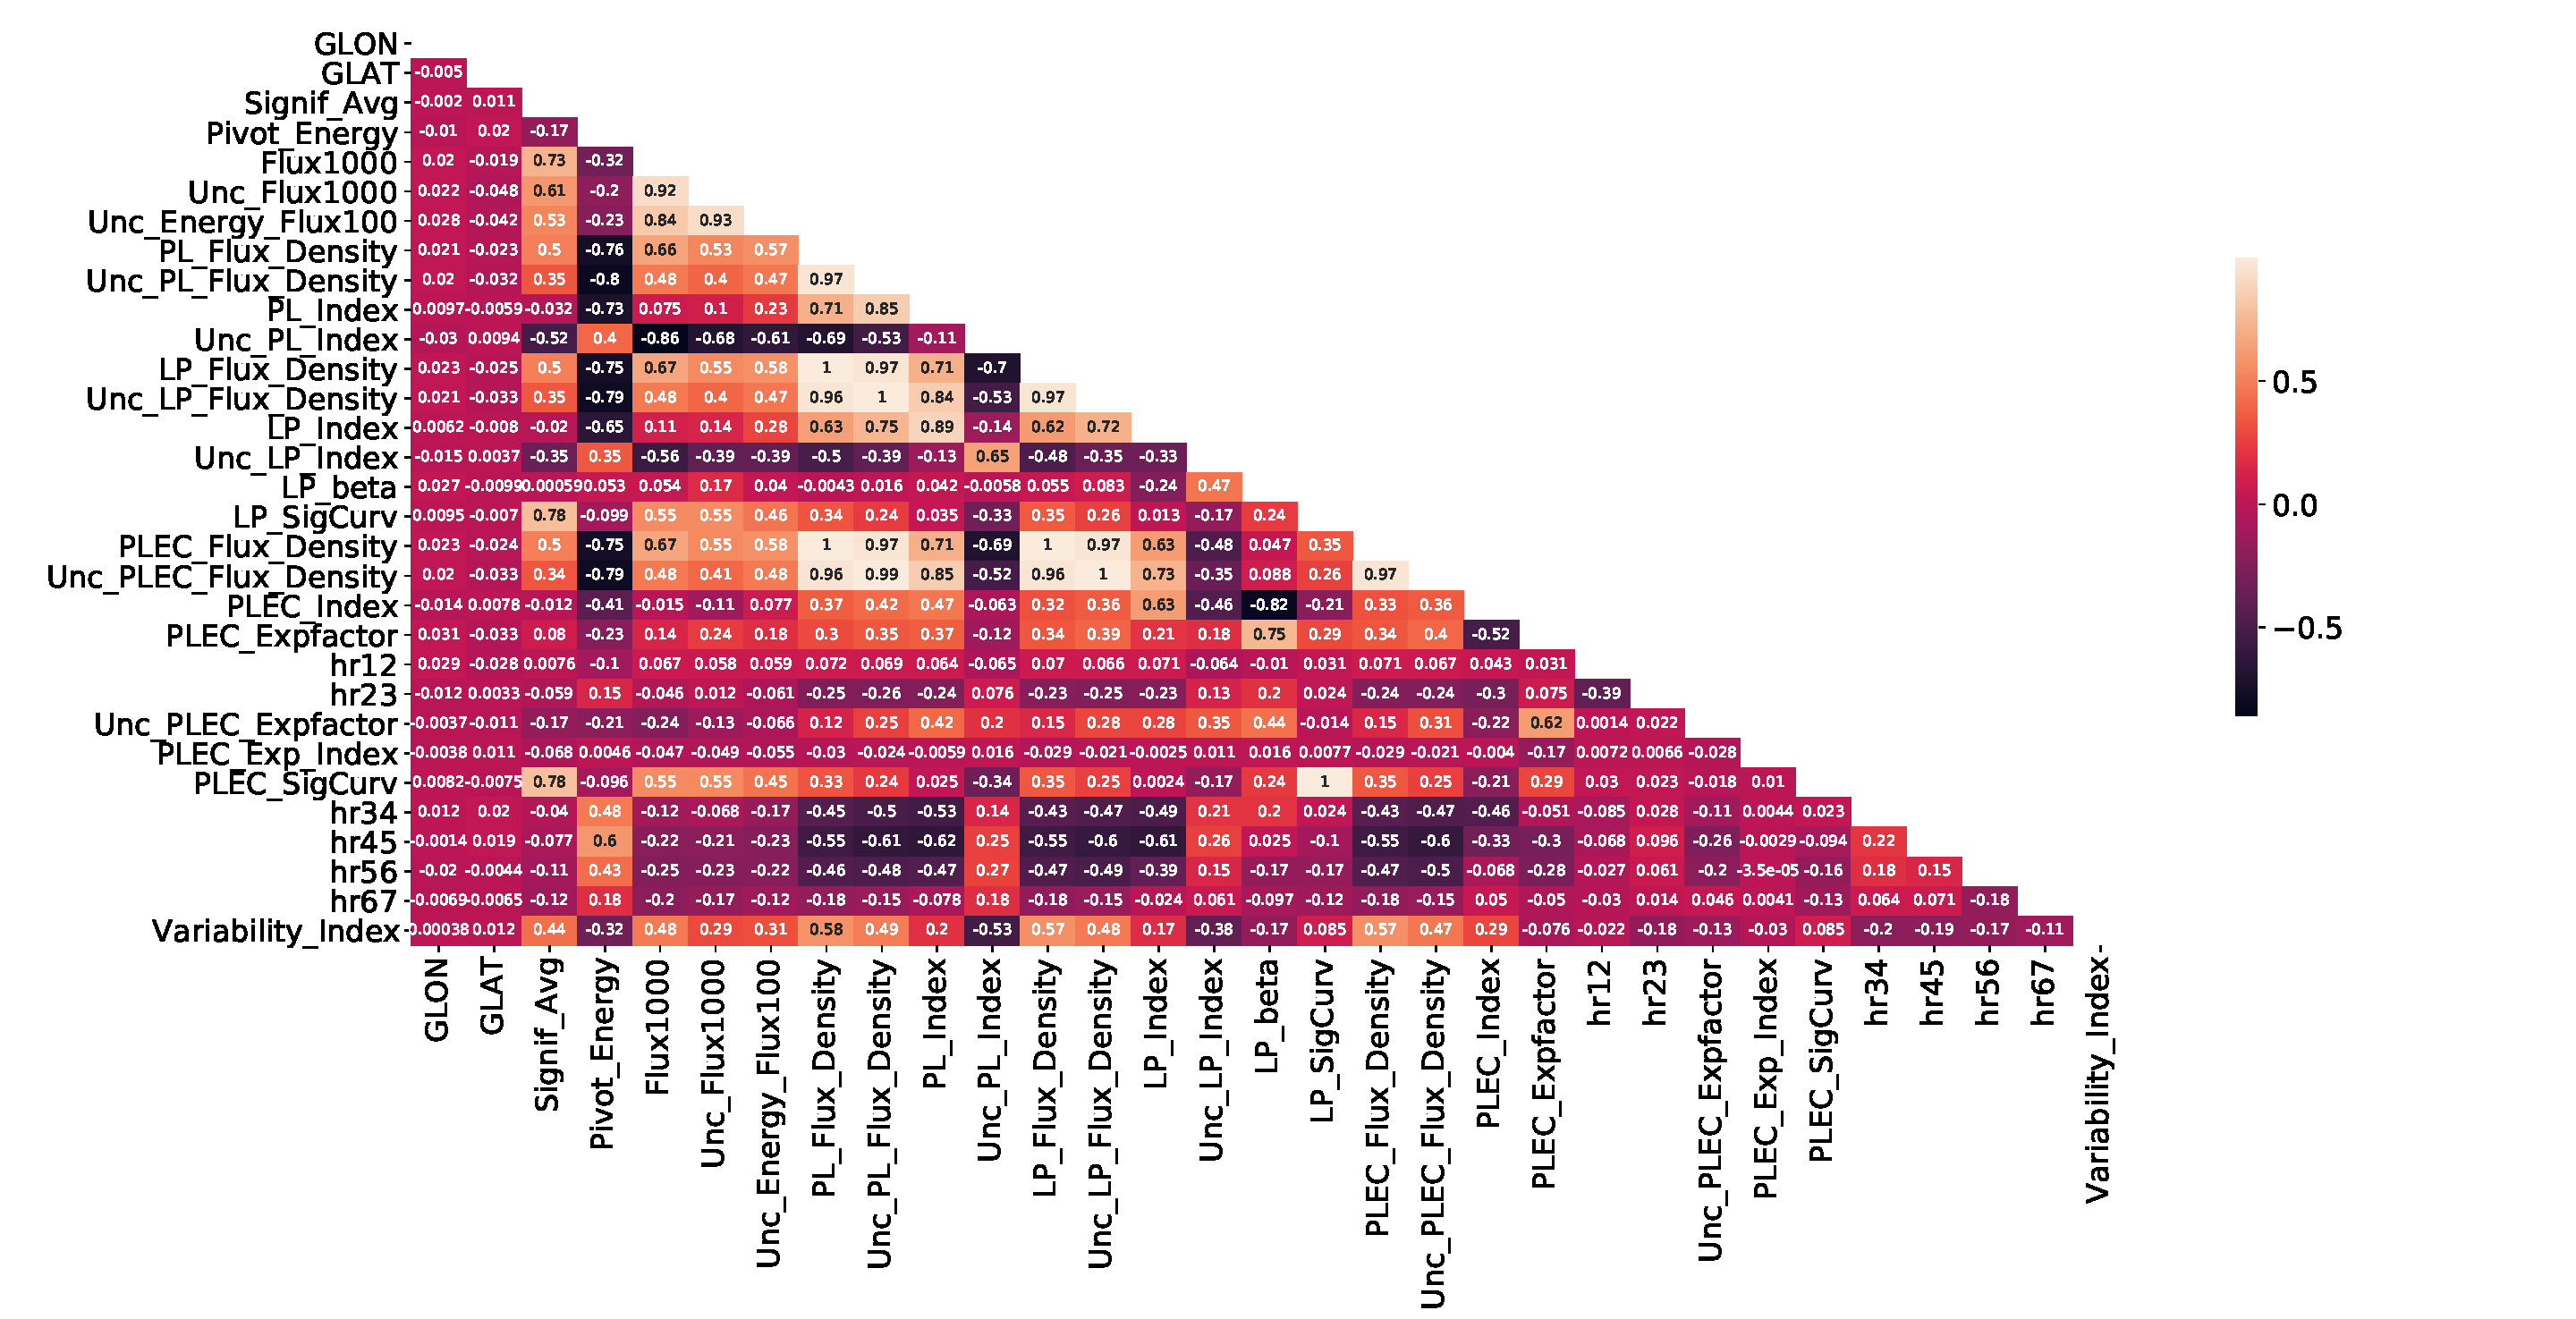
\includegraphics[width=\textwidth]{plots/correlation_4fgl_assoc.pdf}
%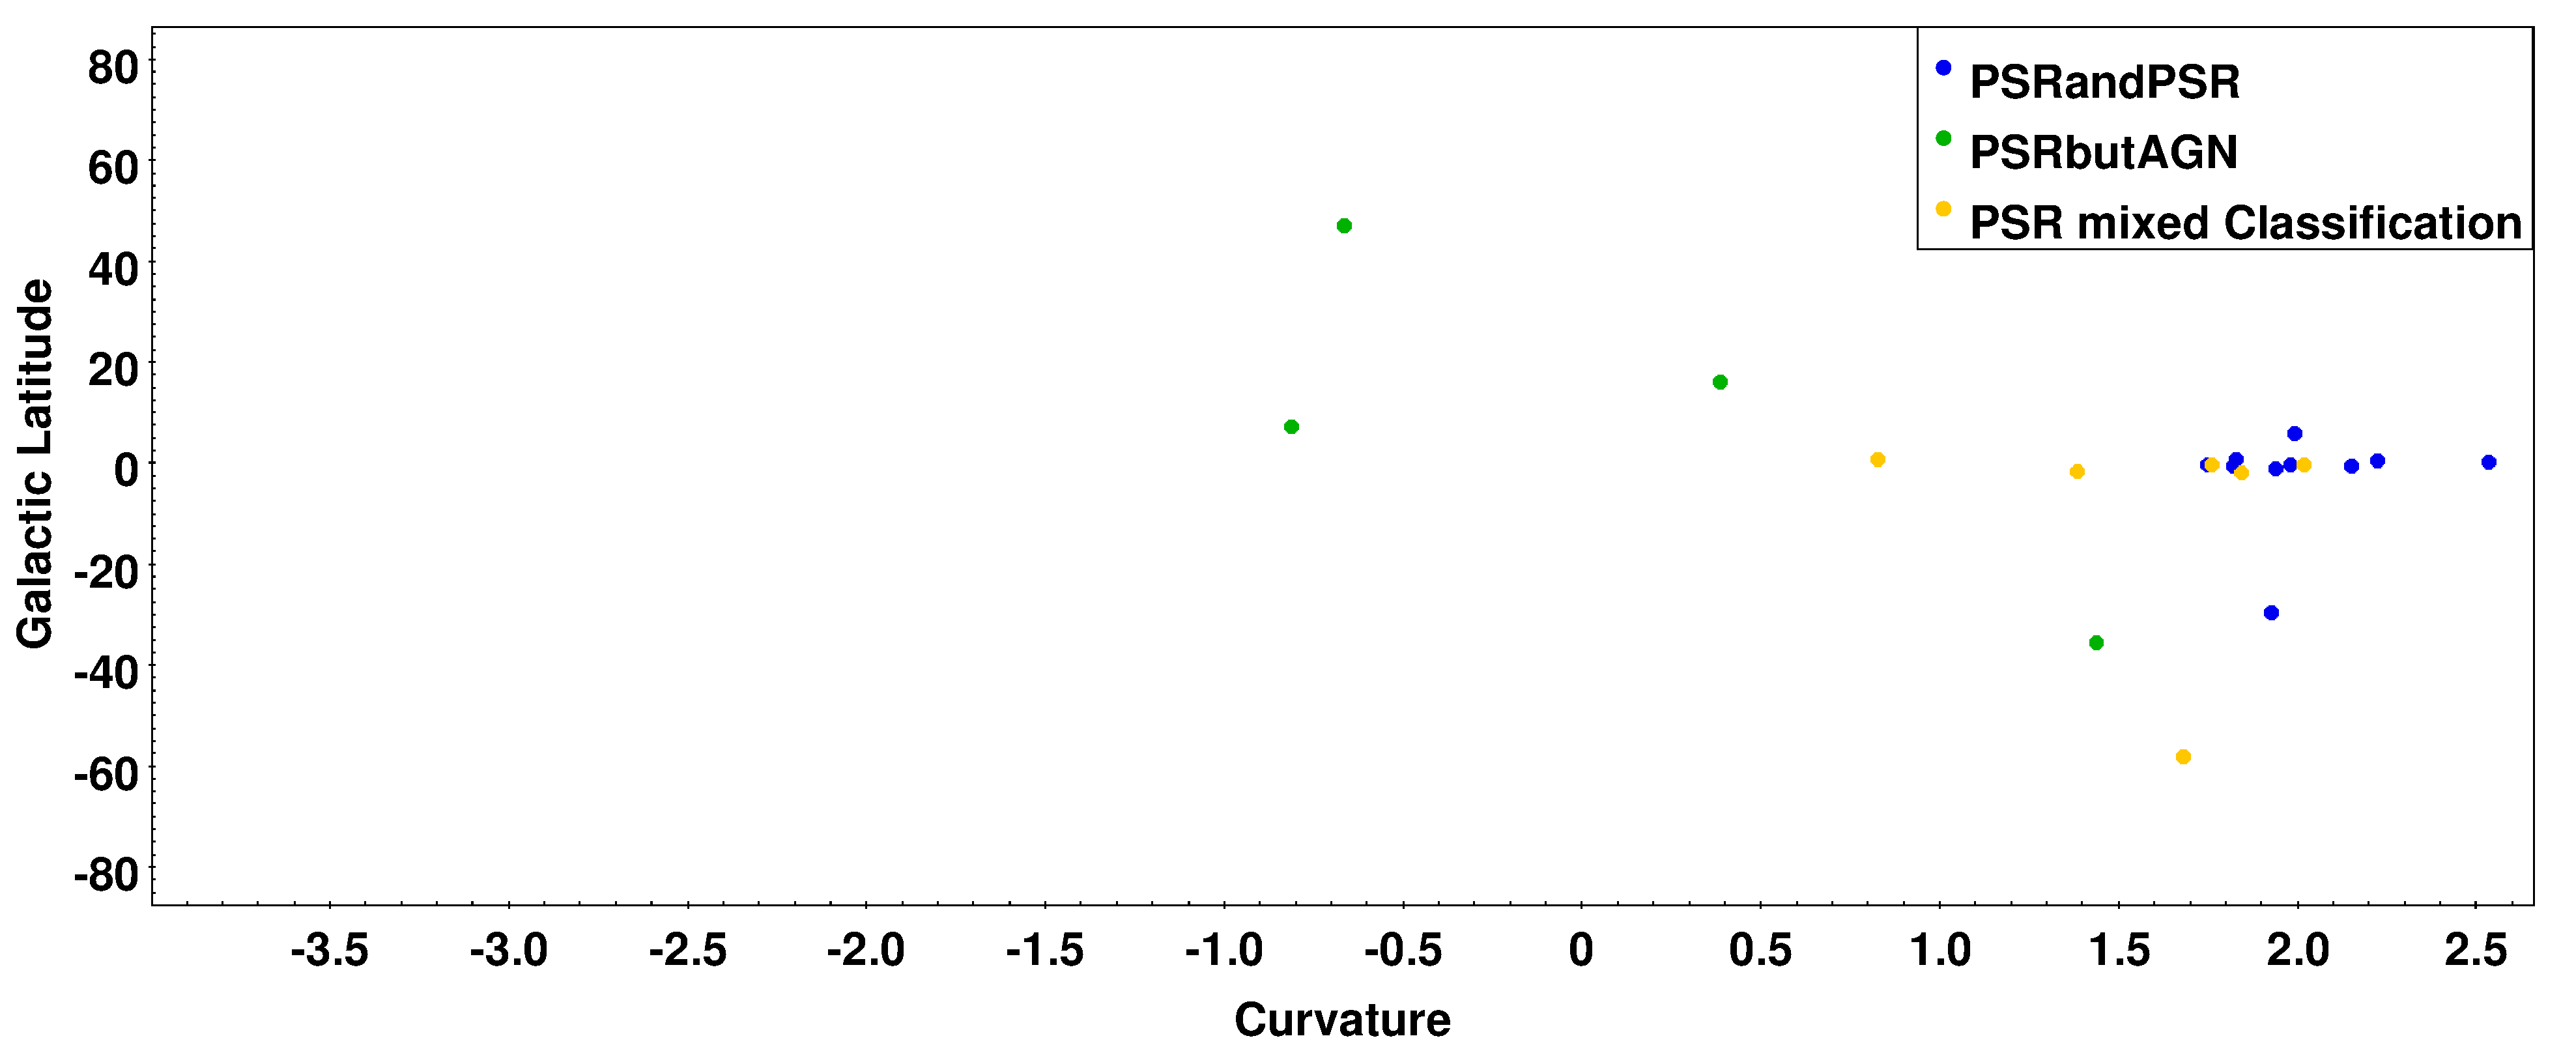
\includegraphics[width=\twopicsp\textwidth]{plots/PSR3.pdf}
\caption{Corelation matrix for 4FGL-DR2 associated data }
%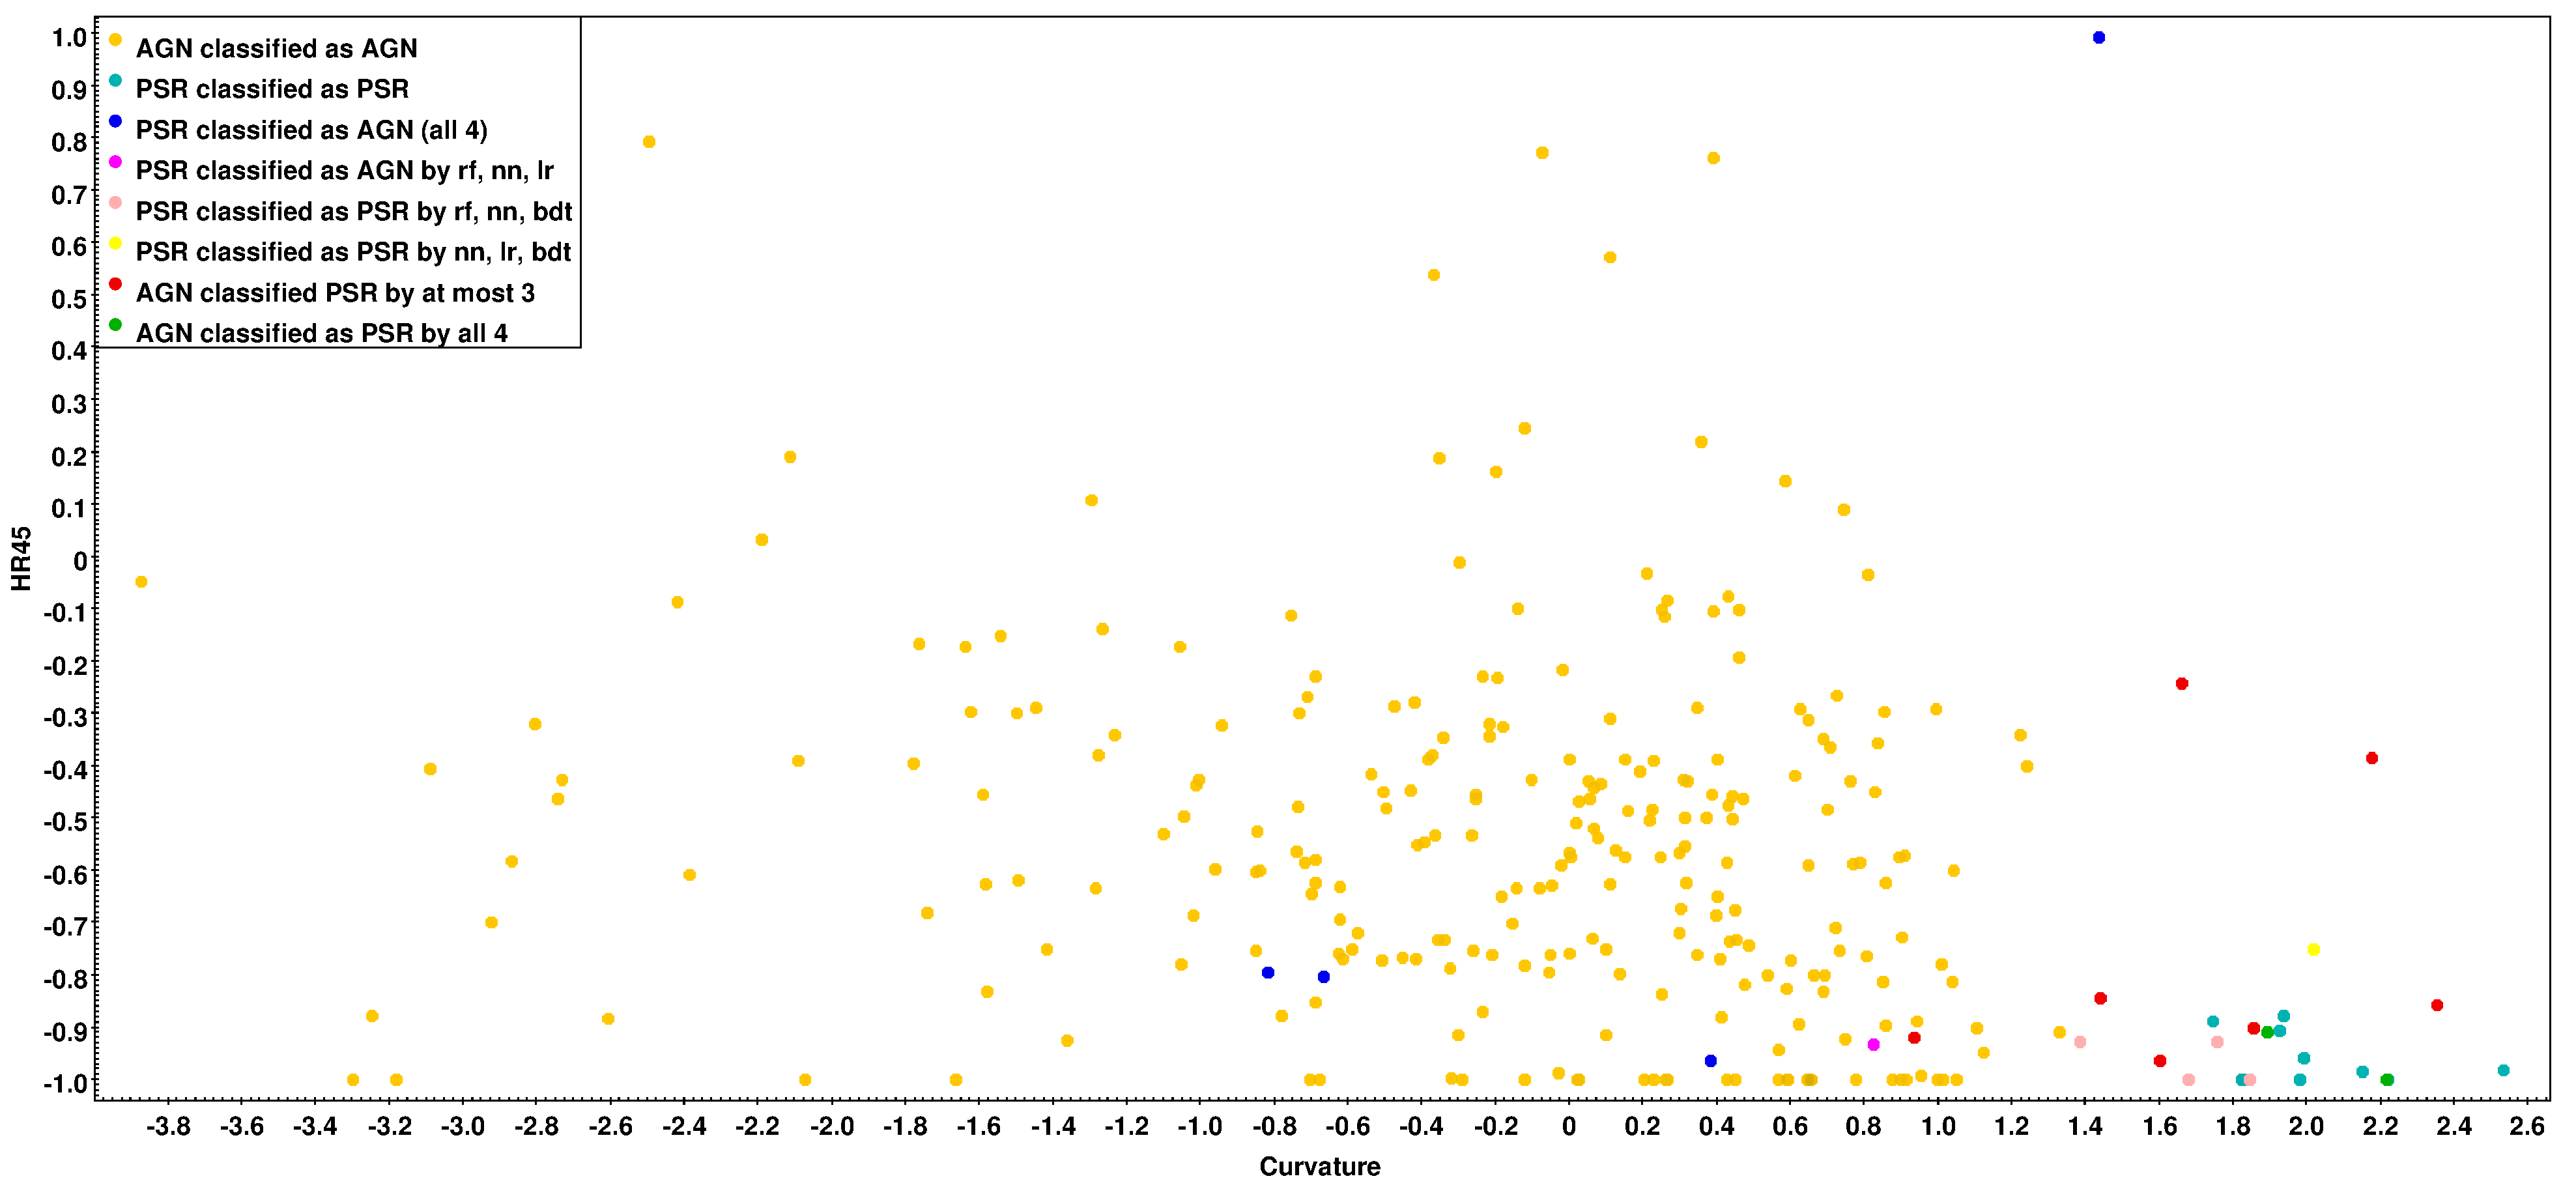
\includegraphics[width=\twopicsp\textwidth]{plots/final_catalog.pdf}
\label{fig:corr_mat}
\end{figure*}
\end{comment}

For the classification of 4FGL-DR2 sources, we confirmed that the parameters used in 3FGL classification provide an optimal performance for the 4FGL-DR2 catalog as well.
Therefore, we used the same meta-parameters for the four algorithms as in the construction of the probabilistic catalog based on 3FGL, except for NN where we increased the number of neurons in the hidden layer to 16. Similar to the construction of the 3FGL probabilistic catalog, we use both unweighted training samples and oversampling, i.e., we have 8 classification methods.
We retrain the algorithms using the 16 features for the 4FGL-DR2 sources.
The corresponding accuracies are reported in Table \ref{tab:selected_algs2}.
All algorithms have a slightly better accuracy for the 4FGL-DR2 catalog compared to the 3FGL catalog, which is likely due to a better determination of the spectra in 4FGL-DR2, to a higher number of features, and more associated sources used as training data. 

% (same as the number of features). However, due to the number of features being higher, we hypothesized that the Neural Network should under-perform as compared to before.

\begin{table}[!h]
\resizebox{0.45\textwidth}{!}{
    \tiny
 %  \centering
    \renewcommand{\tabcolsep}{0.4mm}
\renewcommand{\arraystretch}{1.6}

    \begin{tabular}{|c|c|c|c|}
    \hline
    Algorithm&Parameters & Testing Accuracy & Std. Dev.\\
    \hline
    RF& 50 trees, max depth 6  &97.87 & 0.36\\
    RF\_O   &&97.56&0.39 \\
    \hline %\midrule   -> aakash do you mean this?
    BDT & 100 trees, max depth 2    &   97.63 &0.39\\
    BDT\_O&&97.72&0.38\\
    \hline
    NN & 300 epochs, 16 neurons, LBFGS  & 97.41 & 0.47\\
    NN\_O&&95.48&0.66\\
    \hline
    LR & LBFGS solver, 200 iterations & 97.80&0.38\\
    LR\_O&&96.03&0.53\\
    \hline
     
    \end{tabular}}
    \vspace{0.2cm}
    \caption{Testing accuracy of the 4 algorithms on 4FGL-DR2 associated data. ``\_O'' denotes training with oversampling.}
    \label{tab:selected_algs2}
\end{table}

The expected numbers of pulsars and AGNs among the 1658 unassociated sources in 4FGL-DR2 without missing values are
presented in the 4FGL-DR2 part of Table \ref{tab:prediction_2and3class}.
The definition of rows is the same as in the 3FGL catalog 2-class classification in Section \ref{sec:3FGLprediction1}.


\begin{table}[!h]
\resizebox{0.45\textwidth}{!}{
    \tiny
 %  \centering
    \renewcommand{\tabcolsep}{0.3mm}
\renewcommand{\arraystretch}{1.5}

    \begin{tabular}{| l |c|c|c|}
    \hline
    Correction for other sources & AGNs & Pulsars & Mixed \\
    \hline
    Uncorrected &  872 & 162  &  624 \\
    \hline
    Corrected & 820.8  & 134.6  & 563.2 \\
    \hline
     
    \end{tabular}}
    \vspace{0.2cm}
    \caption{Expected numbers of pulsars and AGNs among unassociated sources in the 4FGL-DR2 catalog \citep{2020arXiv200511208B}.
    For definitions see Table \ref{tab:3FGL_prediction}.}
    \label{tab:4FGL-DR2}
\end{table}


Finally, we looked at sources which were unassociated in both 3FGL and 4FGL-DR2 (using 'ASSOC\_FGL' as an identifier for 3FGL sources). Out of 303 such sources\footnotetext{These are actually 303 4FGL-DR2 sources and 302 3FGL sources with 2 4FGL-DR2 sources associated with 1 3FGL source.}, 40 sources are predicted to be pulsars using 3FGL features and 75 sources are predicted to be pulsars using 4FGL features. This leads to 29 sources which are predicted by all eight methods to be pulsars for features taken from both 3FGL and 4FGL catalogs. 
For convenience, we save these 29 pulsar candidates as a separate file.

Among the 6 unassociated 3FGL sources classified as pulsars and spatially associated with pulsars in the Parkes survey in Table \ref{tab:parkes}, four are unassociated in 4FGL-DR2 and are predicted to be pulsars by the probabilistic classification of unassociated 4FGL-DR2 sources. Of the other two, one is now associated as a pulsar in 4FGL-DR2, and the second one is not detected in 4FGL-DR2. 




\section{Application of probabilistic catalogs for population studies}
\lb{sec:pop_studies}

\subsection{Number of sources as a function of flux}
\lb{sec:dNdS}


In this section we show how probabilistic catalogs can be used, for instance, for population studies.
One of the most important questions in gamma-ray astronomy is contribution of point sources, 
e.g., AGNs, to the extragalactic gamma-ray flux 
\citep[e.g.,][]{2010ApJ...720..435A, 2011ApJ...738..181M, 2016PhRvL.116o1105A, 2016ApJS..225...18Z, 2016ApJ...826L..31Z, 2016ApJ...832..117L, 2018ApJ...856..106D}:
if most of the extra-galactic emission is explained by point sources, then one can put stringent constraints, 
e.g., on  dark matter annihilation or decay into gamma rays 
\citep{2015ApJ...800L..27A, 2015PhRvD..91l3001D, 2015JCAP...09..008F, 2015PhR...598....1F, 2017ChPhC..41d5104L} or 
on evaporation of primordial black holes \citep{2010PhRvD..81j4019C}.
In particular, it is important to understand the contribution to the population of AGNs from the unassociated sources.
A probabilistic catalog provides an answer to the question: how many sources among the unassociated ones are expected to belong to different classes, such as pulsars or AGNs. 
One can calculate the total expected number of AGNs or pulsars among the unassociated sources, or calculate the contribution as a function of one or more parameters.
In this section we determine the numbers of AGNs and pulsars as a function of their flux.



\begin{figure*}[h]
\center
%\hspace*{-1cm}
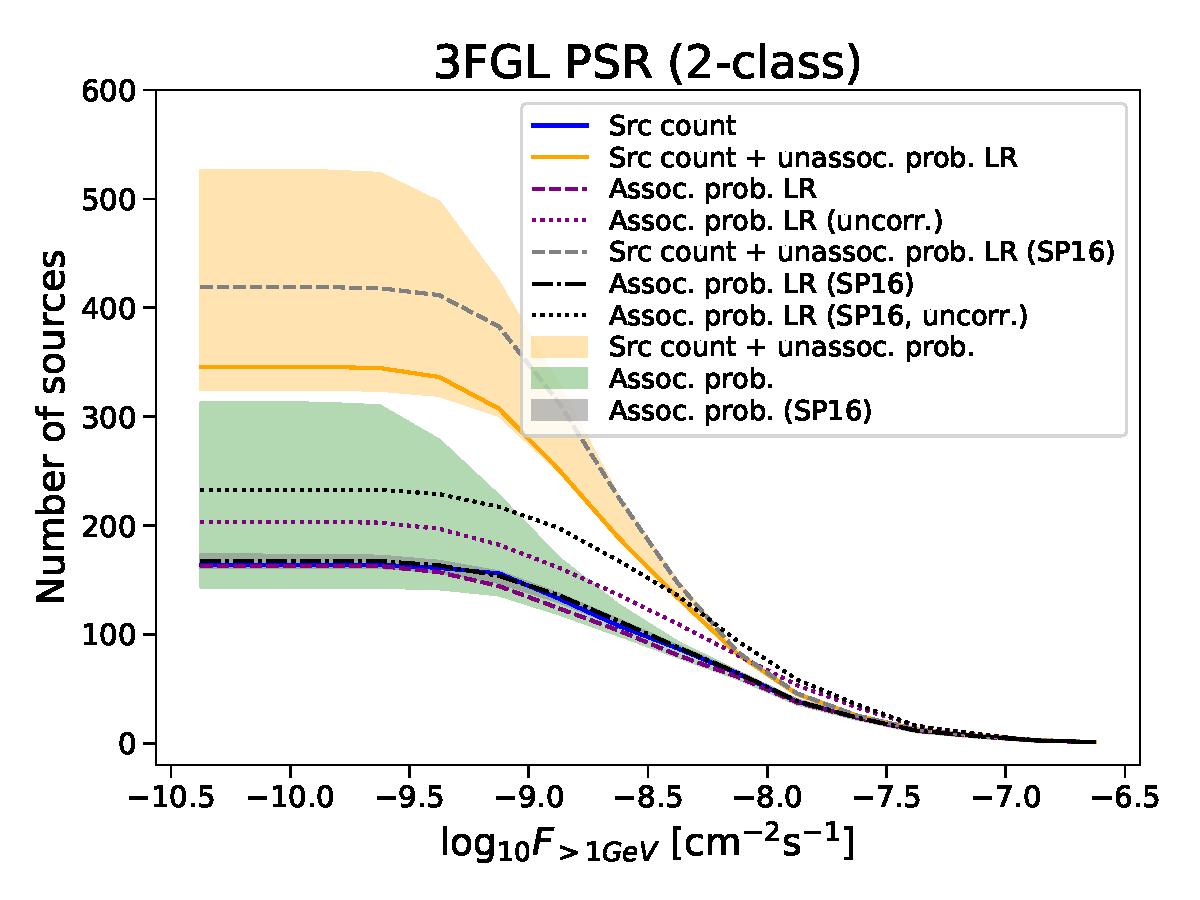
\includegraphics[width=0.45\textwidth]{plots/N_logS_3FGL_PSR_SazP_add_os.pdf}
%\hspace*{-1cm}
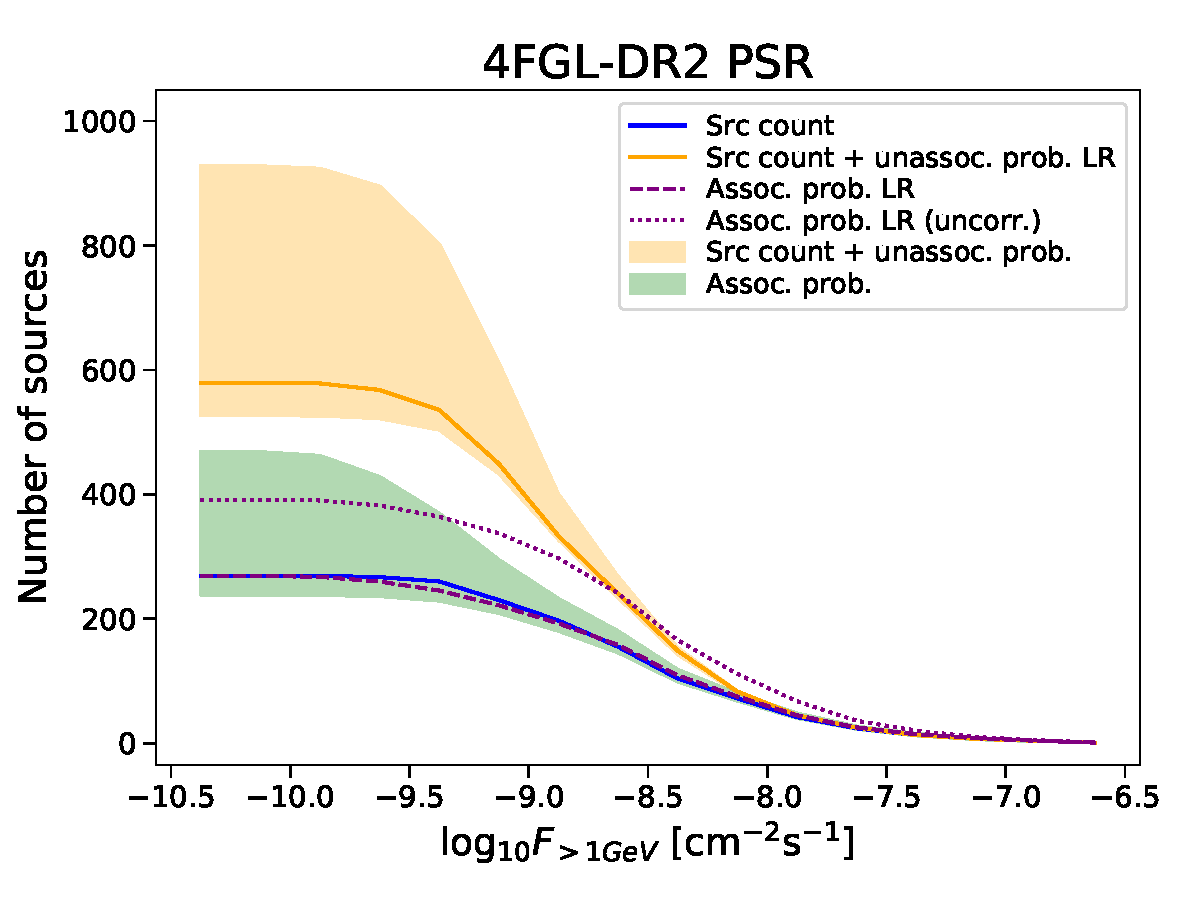
\includegraphics[width=0.45\textwidth]{plots/N_logS_4FGL-DR2_PSR_add_os.pdf} \\
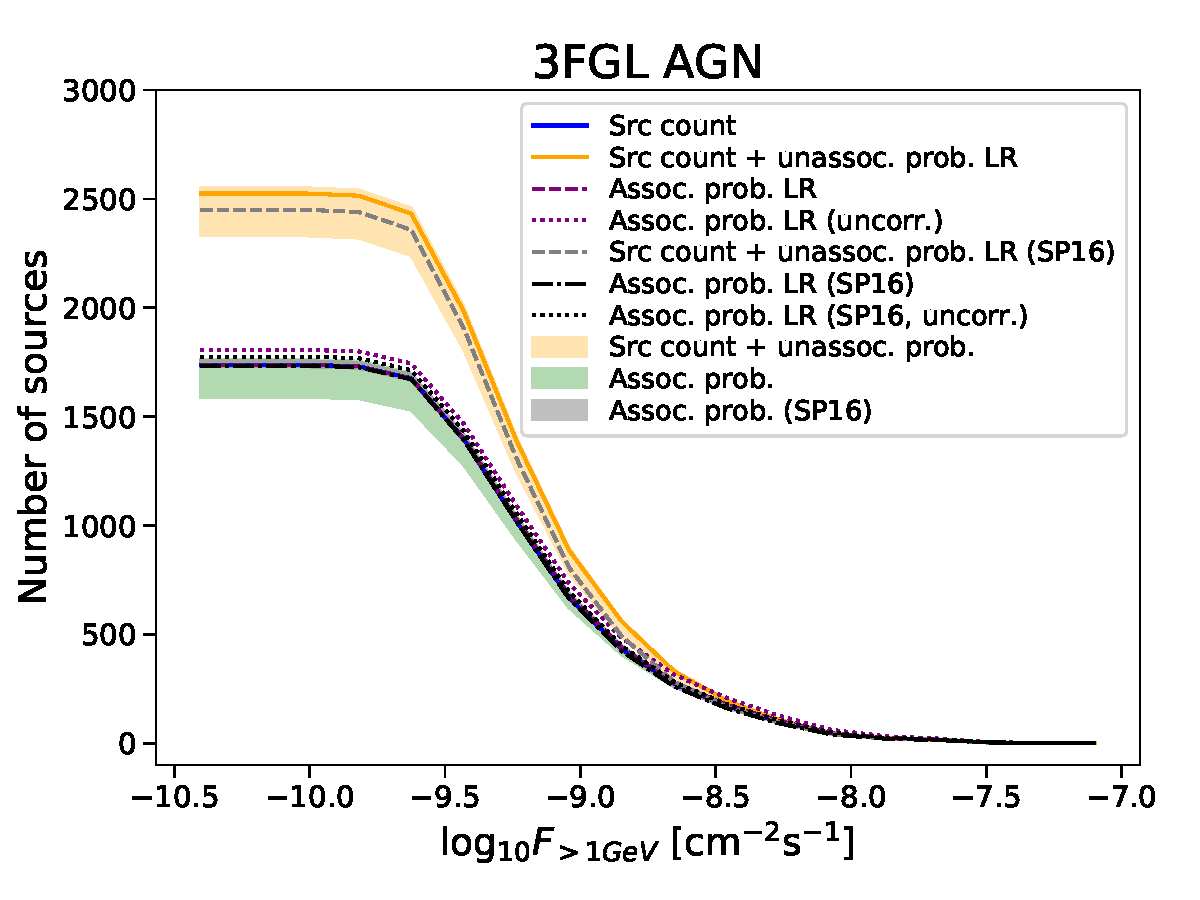
\includegraphics[width=0.45\textwidth]{plots/N_logS_3FGL_AGN_SazP_add_os.pdf}
%\hspace*{-1cm}
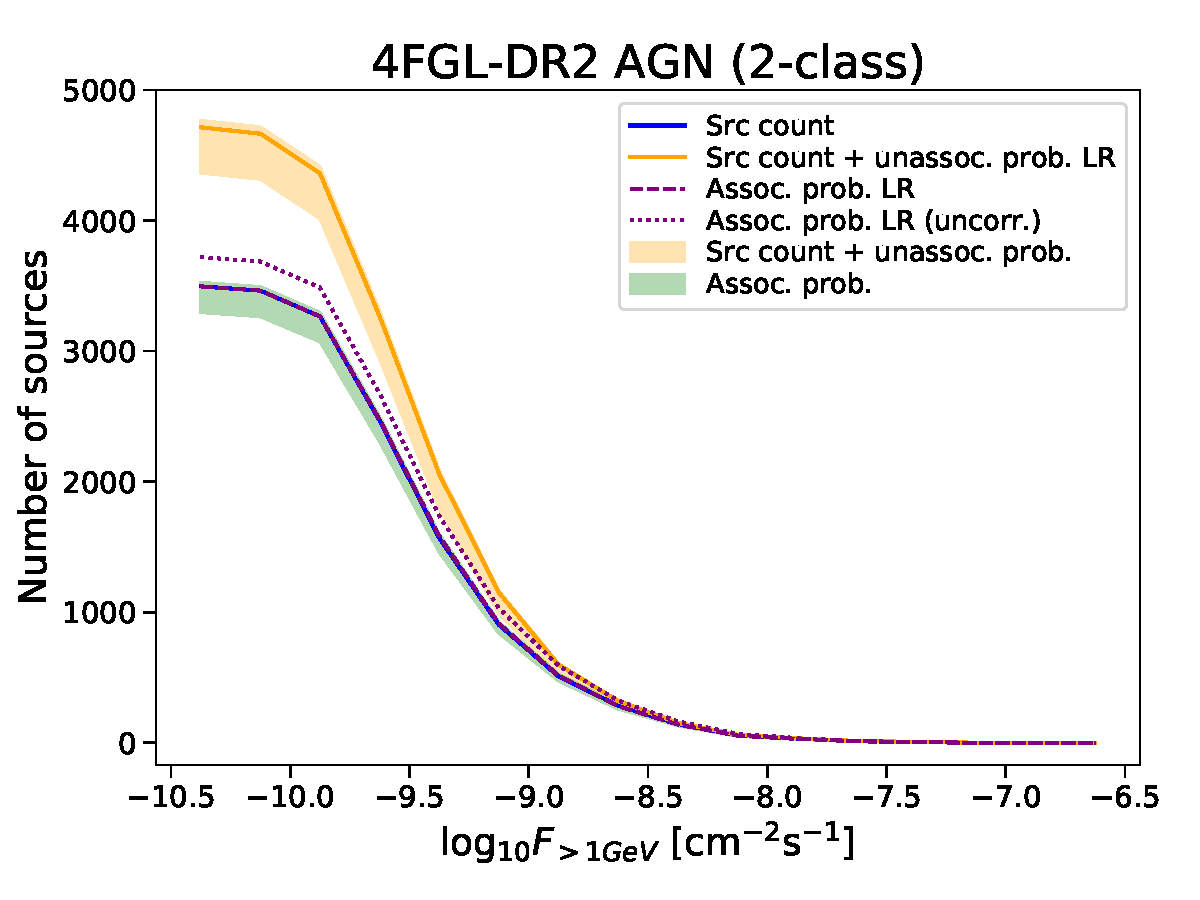
\includegraphics[width=0.45\textwidth]{plots/N_logS_4FGL-DR2_AGN_add_os.pdf}
\caption{Cumulative number of sources as a function of their flux. Green bands show the envelope of the sum of class probabilities for associated sources, while orange bands show the sum of counts of associated sources (blue solid line) plus the sum of probabilities for unassociated sources. The curves with ``SP16'' in the labels are derived from the data in \cite{2016ApJ...820....8S}. For details see Section \ref{sec:dNdS}.}  
\label{fig:logN_logS}
\end{figure*}


\begin{figure}[h]
\center
%\hspace*{-1cm}
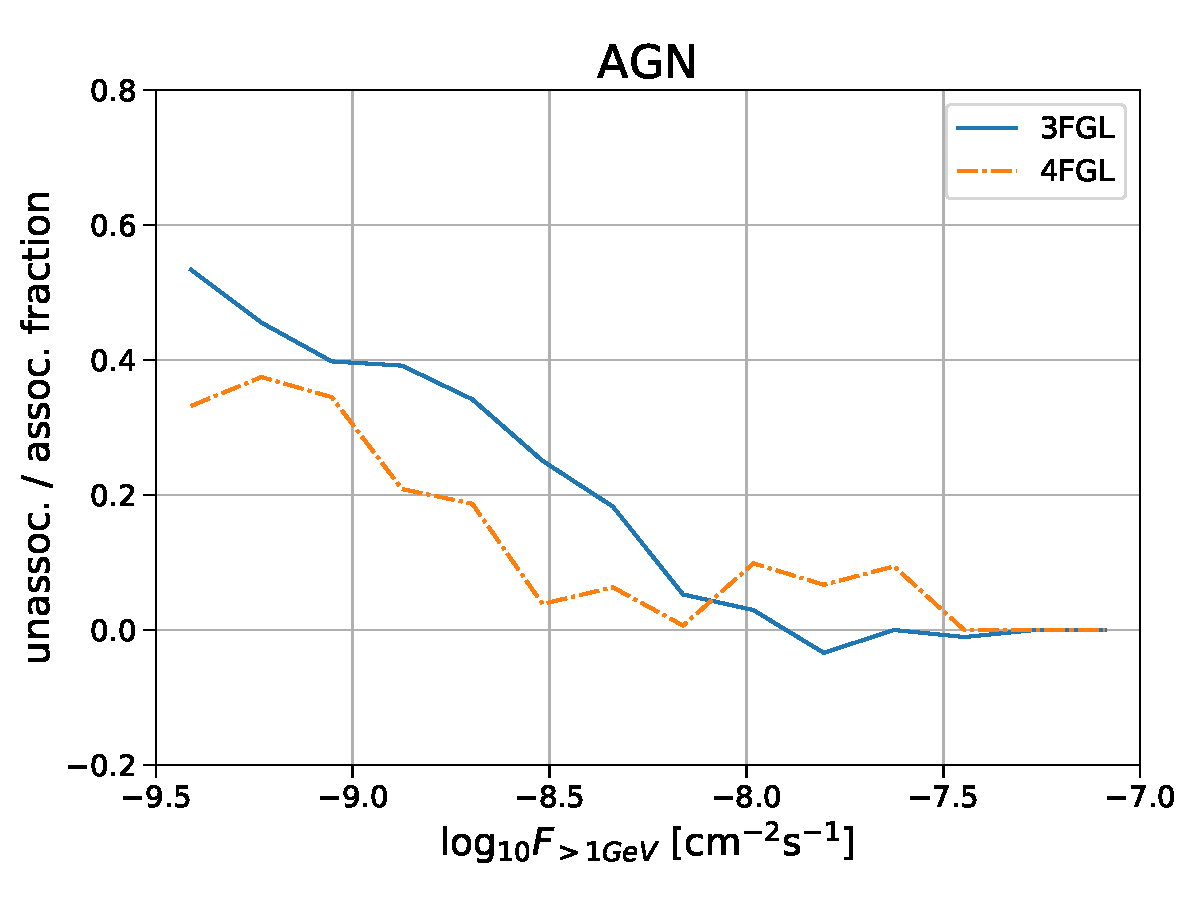
\includegraphics[width=0.45\textwidth]{plots/N_logS_diff_AGN.pdf}
%\hspace*{-1cm}
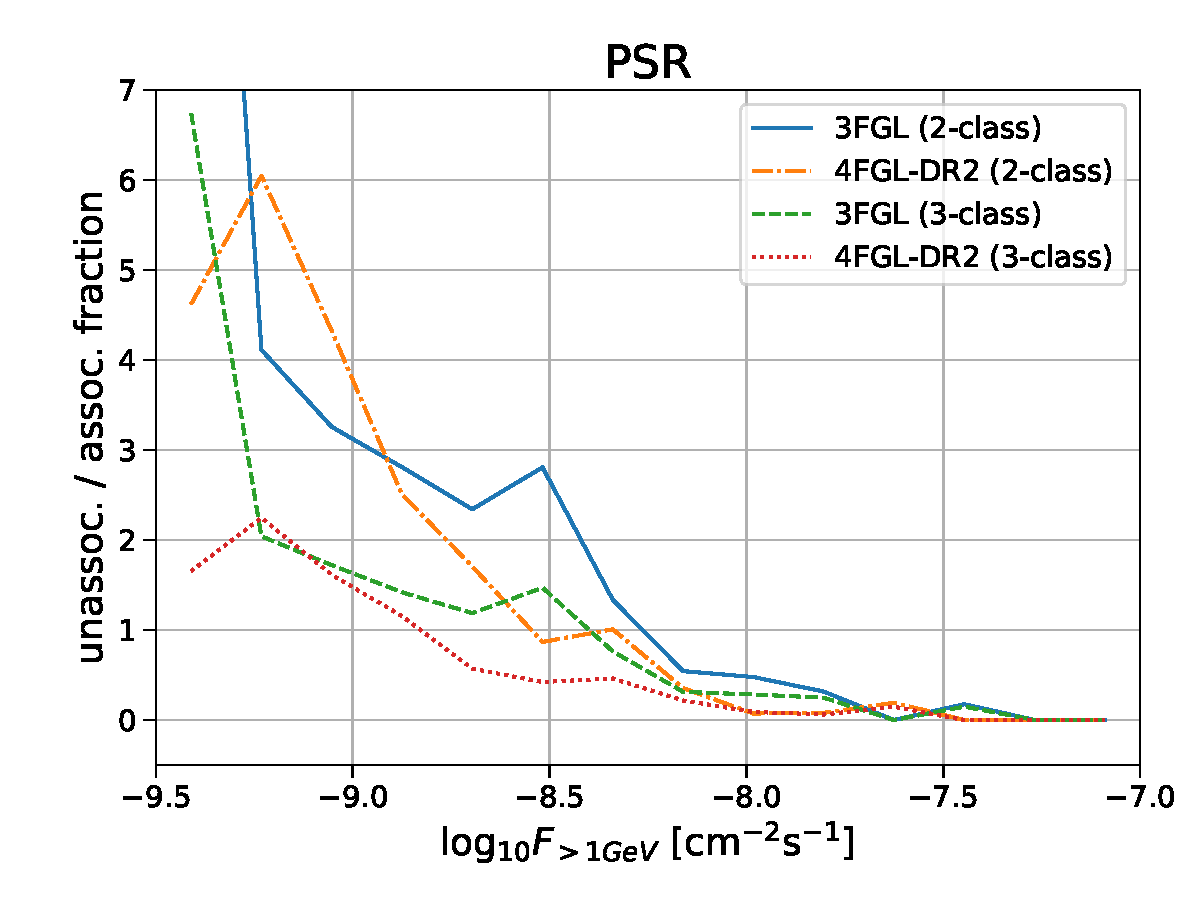
\includegraphics[width=0.45\textwidth]{plots/N_logS_diff_PSR.pdf}
\caption{Ratio of estimated number of AGNs and pulsars among unassociated sources corrected for the presence of other sources (Equation (\ref{eq:unassoc_ev})) to the counts of associated AGNs and pulsars respectively.}  
\label{fig:unass_vs_ass_frac}
\end{figure}




In Figure \ref{fig:logN_logS} we show the cumulative number of AGNs and pulsars with flux above 1 GeV larger than the
value on the x-axis.
Solid blue lines show the actual counts of sources (AGNs or pulsars) in the 3FGL and 4FGL catalogs.
As a consistency check of the method, we calculate the AGN- and PSR-like probabilities for associated sources.
The sum of probabilities (uncorrected for sources other than AGNs and pulsars) for LR algorithm are shown by dotted purple lines.
In order to correct the expected number of AGNs among associated sources for AGN-like probabilities in ``other'' sources, 
we subtract the corresponding AGN-like probabilities in each flux band:

\be
\lb{eq:assoc_ev}
N_{\rm AGN}^{\rm ass}  = \sum_{i \in \rm ass} p^i_{\rm AGN}\,\, - \sum_{i \in \rm ass\,other} p^i_{\rm AGN}.
\ee
The corrected sums of probabilities for LR method are shown by dashed purple lines.
The green bands show the envelope of the sums of corrected probabilities for the eight methods used in this paper.
We see that the counts of associated sources, AGNs and pulsars, are consistent with the expected number of associated sources
calculated from the class probabilities of associated sources.
This conclusion is not very surprising since we used associated sources for training of ML algorithms.
It is important to note that correction for ``other'' sources is important for consistency of the sum of probabilities and the number of associated sources.
We have also compared the sums of probabilities for the 3FGL associated sources in \cite{2016ApJ...820....8S}.
%\footnote{The data is downloaded from \url{https://www.physics.hku.hk/~pablo/pulsarness.html}.} !!! resolve the footnote issue?
The sum of probabilities for associated sources in the LR case uncorrected for ``other'' sources are shown by dotted black line,
while the sums corrected for ``other'' sources are shown by black dash-dotted lines.
The gray band is the envelope of the two methods (LR and RF) used by \cite{2016ApJ...820....8S}.
We see that the sum of probabilities for pulsars overpredicts the pulsar counts in 3FGL, 
while correction for ``other'' sources makes the prediction consistent with the counts of pulsars.

The predictions for the number of AGNs and pulsars among the unassociated sources corrected for ``other'' sources 
added to the 3FGL and 4FGL source counts are shown by solid orange lines (for the LR case).
The orange bands show the corresponding envelopes for the eight ML methods.
We assume that the fractional contribution of other sources is the same for associated and unassociated sources in the different flux bands.
Thus, the correction for the presence of other sources is calculated similarly to the associated sources in Equation \ref{eq:assoc_ev},
but we adjust for the fact that there are fewer unassociated than associated sources, i.e., 
the correction is assumed to be proportionally smaller.
In particular, the number of AGNs among unassociated sources in a flux band $\Delta F$ is estimated as

\be
\lb{eq:unassoc_ev}
N_{\rm AGN}^{\rm unass} = \sum_{i \in \rm unass} p^i_{\rm AGN}\,\, - \sum_{i \in \rm ass\,other} p^i_{\rm AGN} \cdot 
\frac{N_{\rm unass}}{N_{\rm ass}}
\ee
where all probabilities and the numbers of sources are computed for sources with flux inside $\Delta F$.
The first term is the sum of AGN-like probabilities among the unassociated sources,
while the second term is the sum of AGN-like probabilities among associated ``other'' sources rescaled by the total number
of unassociated and associated sources in this flux band.
The expected number of pulsars among the unassociated sources is calculated analogously.
The corresponding sums of associated source counts plus the expected number of sources calculated with LR method of \cite{2016ApJ...820....8S} 
and corrected for other sources are shown by dashed grey lines.


We predict that the expected number of pulsars among the unassociated sources in the 3FGL catalog
is $267 \pm 110$, where the range is the envelop of the sums of probabilities in Equation (\ref{eq:unassoc_ev})
for different ML methods (including oversampling) corrected for other sources among the unassociated sources.
The expected number of pulsars among the unassociated sources in the 4FGL catalog corrected for other sources is 
$386 \pm 179$.
These numbers are larger than the number of associated PSRs without missing values (164 in 3FGL and 237 in 4FGL).
Even at the lower range of expected numbers of pulsars among unassociated sources, there are potentially as many pulsars
as there are associated ones.

We note that according to Table \ref{tab:3FGL_prediction}, the number of unassociated 3FGL sources 
with $p_{\rm PSR} > 0.5$ for all four ML algorithms is 96 (83), while there are 332 (309.5) sources with mixed classification,
uncorrected (corrected) for other sources.
The number of sources with mixed classification (309.5 for 3FGL or 475.5 for 4FGL)
is larger than the range of values for the expected number of pulsars calculated for the sum of probabilities 
(220 for 3FGL or 358 for 4FGL).
It means that the decision which sources are considered to be more likely pulsars is more sensitive to the choice of the ML method
and the probability threshold than the expected number of pulsars calculated from the sum of probabilities.

We also note that the probabilistic classification mostly affects sources with smaller fluxes,
which we illustrate in Figure \ref{fig:unass_vs_ass_frac}, where we show that the ratio of expected number of AGNs and pulsars among 
unassociated sources computed according to Eq. \ref{eq:unassoc_ev} using LR method without oversampling to the number of associated 
sources decreases as the flux increases.
Negative values (e.g., at high fluxes for AGNs) are due to subtraction of probabilities for the ``other'' associated sources.

\begin{figure*}[h]
\center
%\hspace*{-1cm}
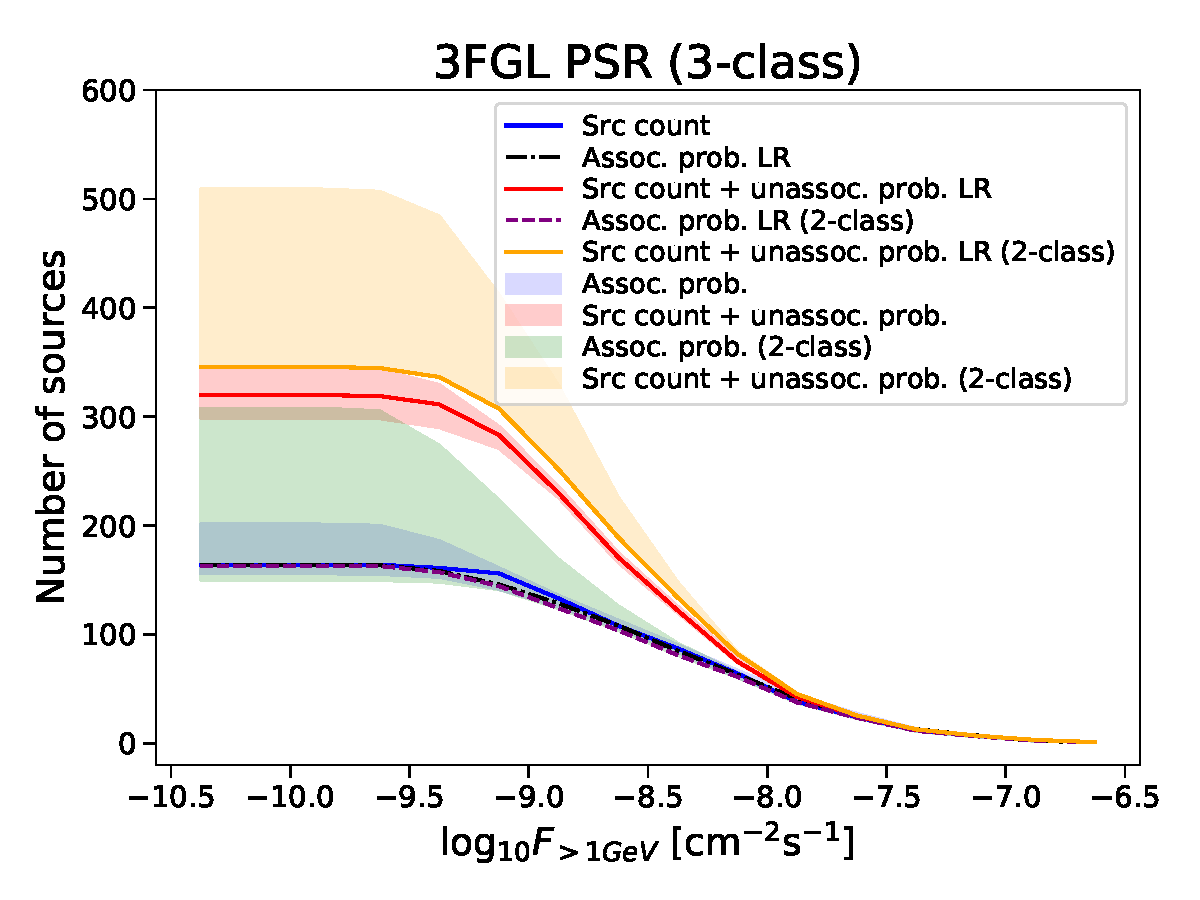
\includegraphics[width=0.45\textwidth]{plots/N_logS_3FGL_PSR_3classes.pdf}
%\hspace*{-1cm}
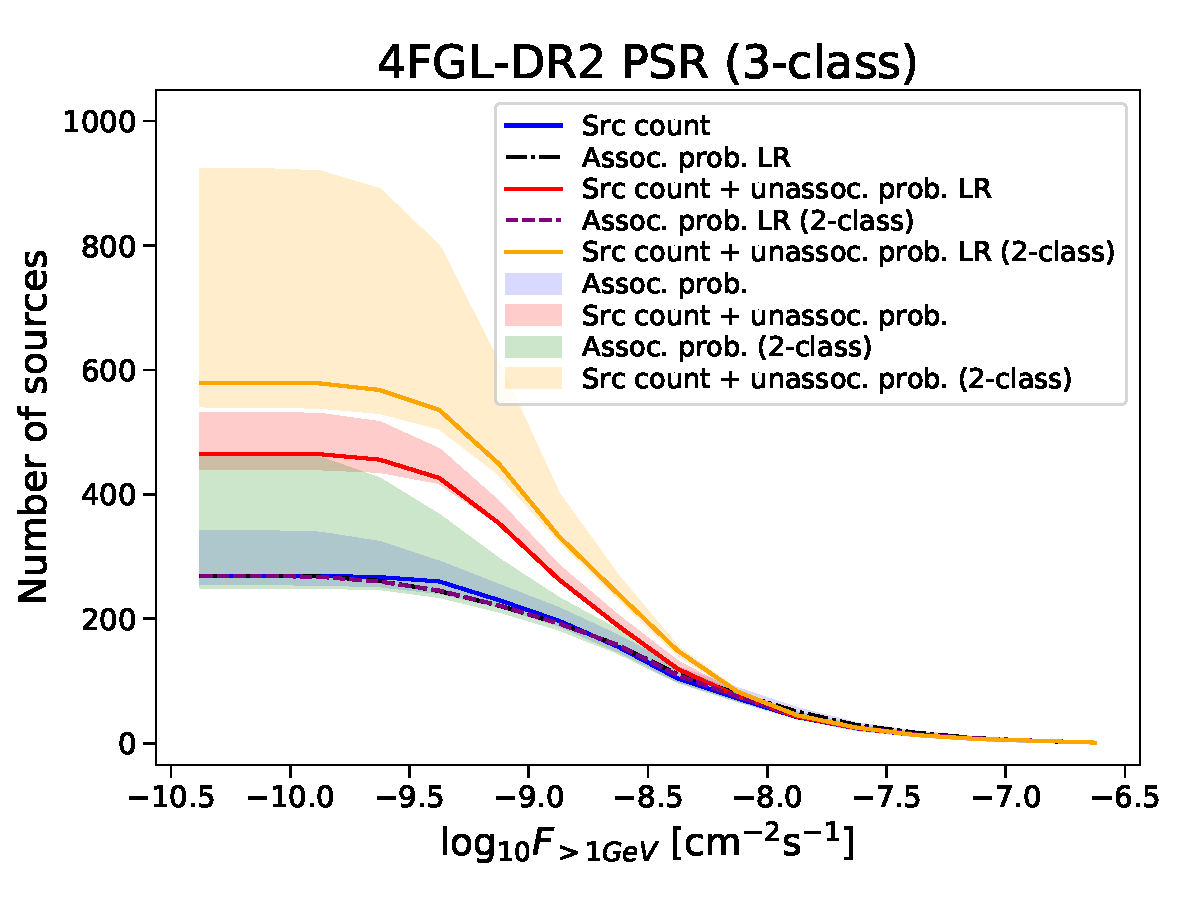
\includegraphics[width=0.45\textwidth]{plots/N_logS_4FGL-DR2_PSR_3classes.pdf} \\
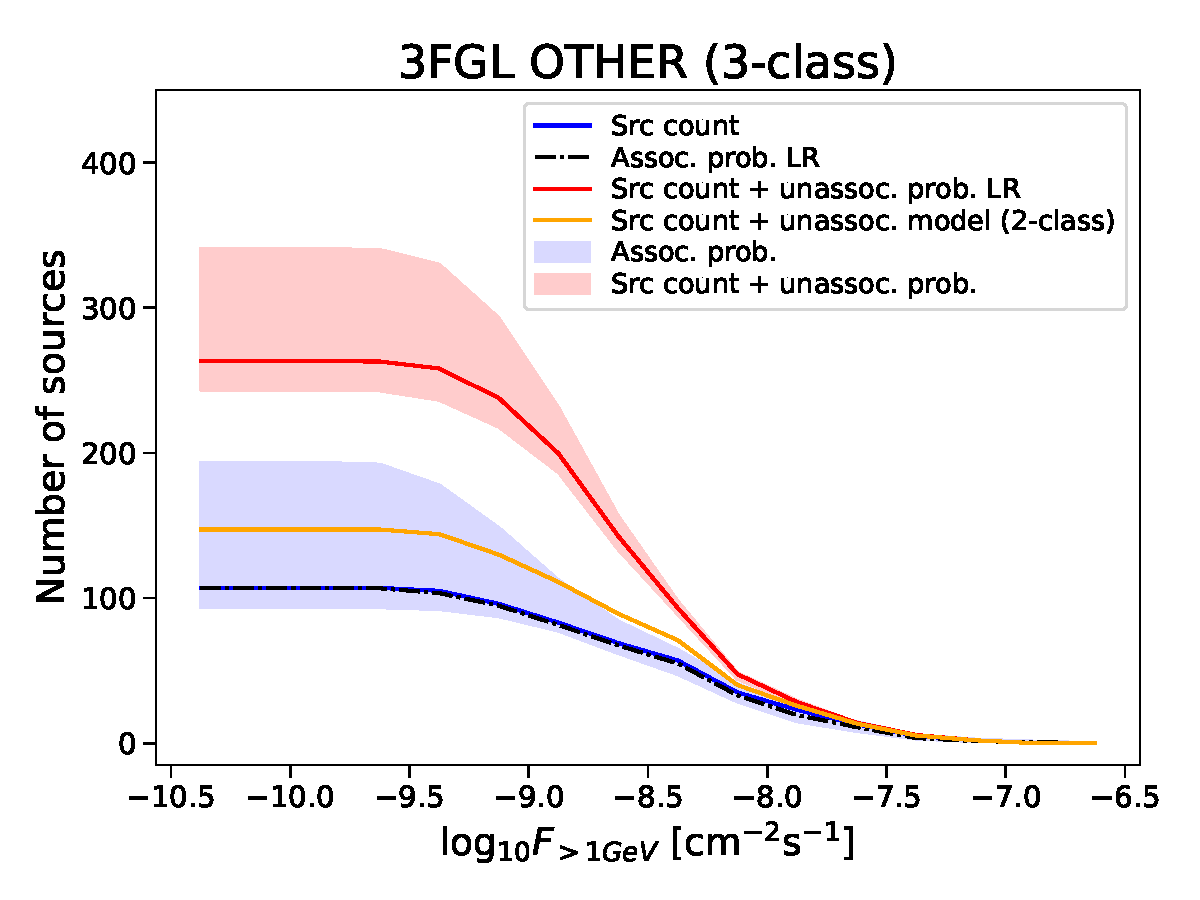
\includegraphics[width=0.45\textwidth]{plots/N_logS_3FGL_OTHER_3classes.pdf}
%\hspace*{-1cm}
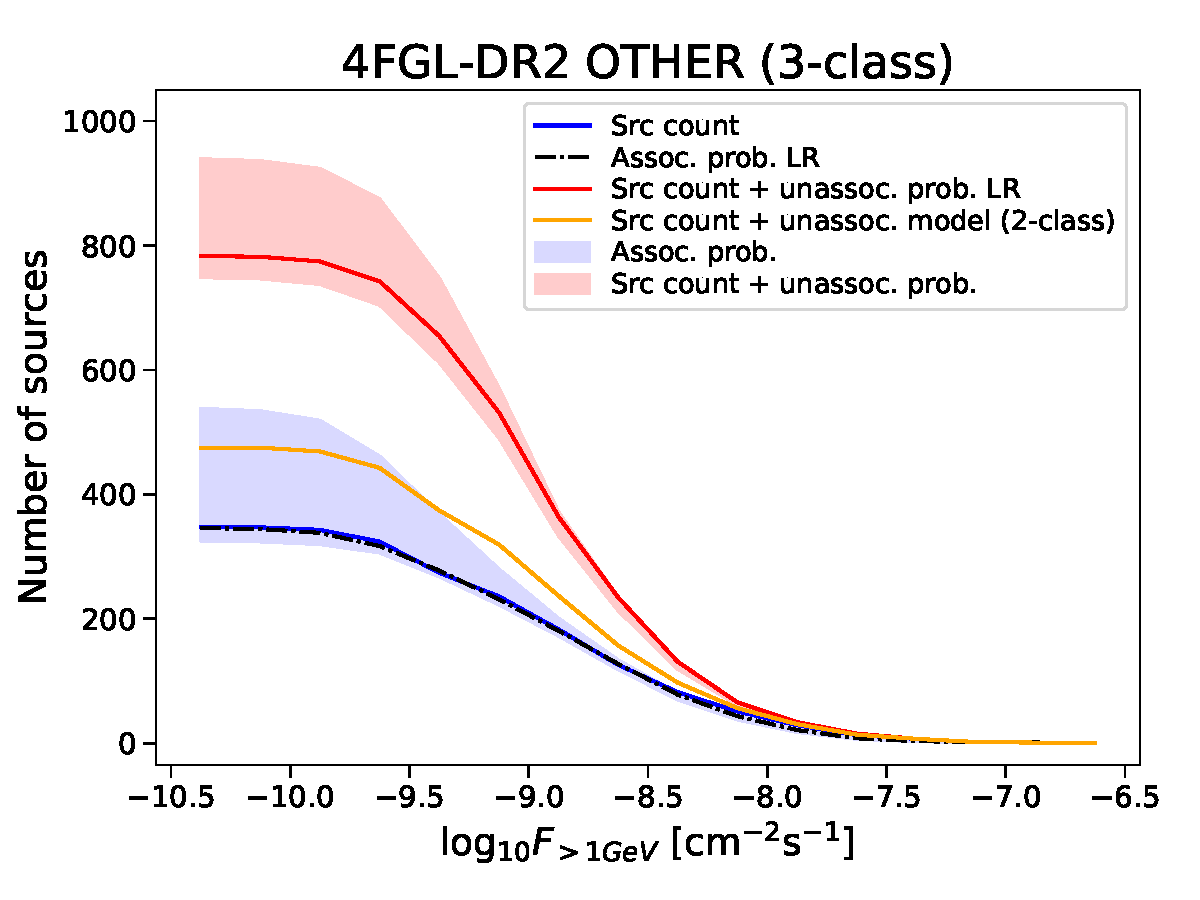
\includegraphics[width=0.45\textwidth]{plots/N_logS_4FGL-DR2_OTHER_3classes.pdf}
\caption{Cumulative number of sources as a function of their flux. Green bands show the envelope of the sum of class probabilities for associated sources, while orange bands show the sum of counts of associated sources (blue solid line) plus the sum of probabilities for unassociated sources. The curves with ``SP16'' in the labels are derived from the data in \cite{2016ApJ...820....8S}. For details see Section \ref{sec:dNdS}.}  
\label{fig:logN_logS_3classes}
\end{figure*}


\subsection{Latitude and longitude profiles}
\lb{sec:lat-lon-profiles}

\begin{figure*}[h]
\center
%\hspace*{-1cm}
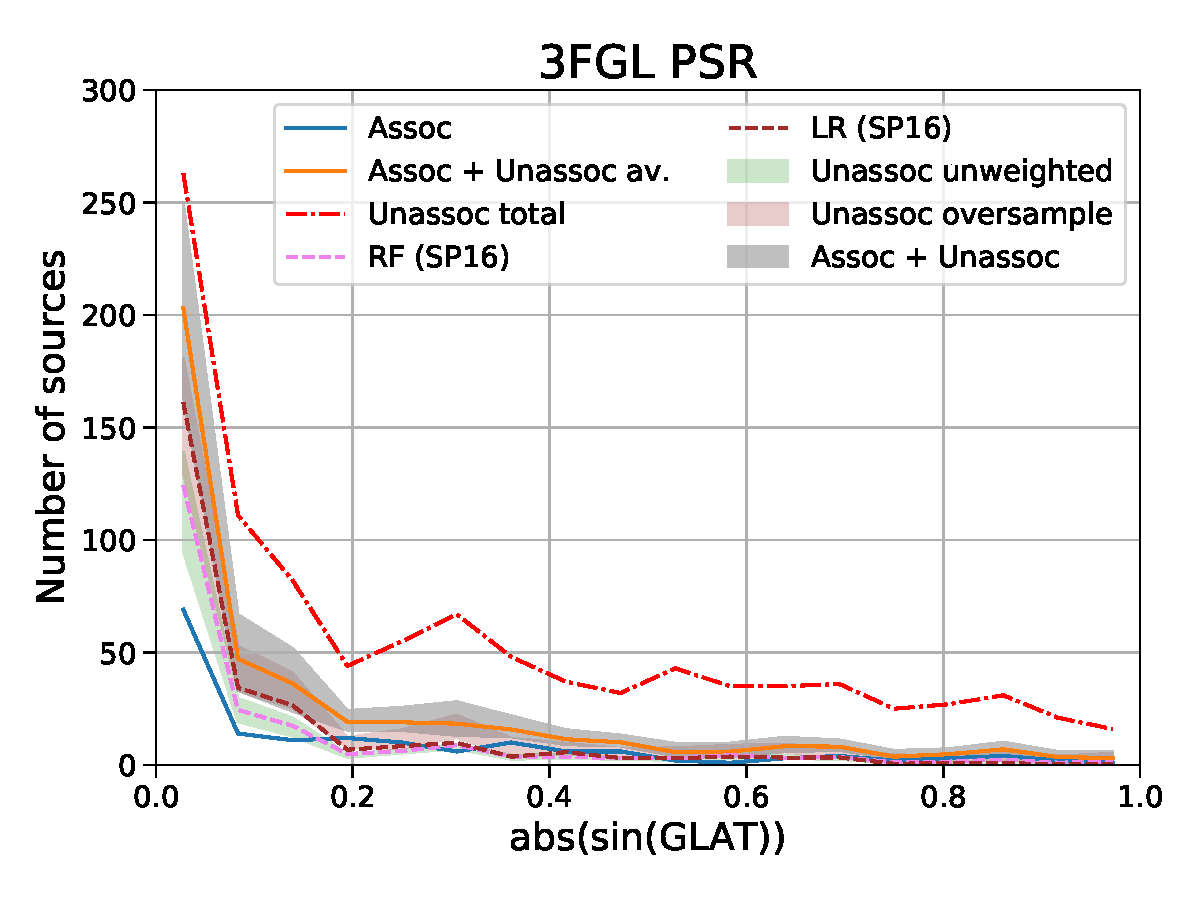
\includegraphics[width=0.45\textwidth]{plots/lat_profile_PSR_3FGL_oversample.pdf}
%\hspace*{-1cm}
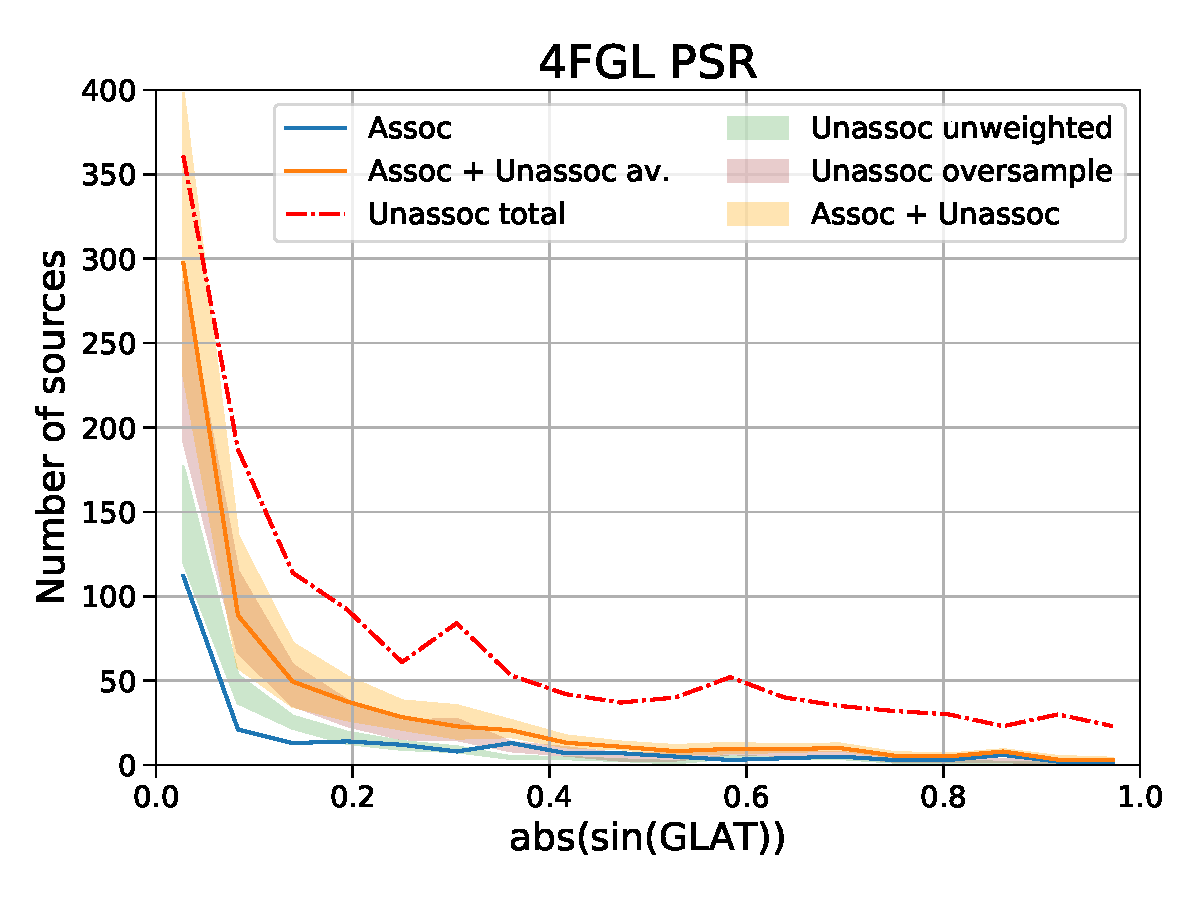
\includegraphics[width=0.45\textwidth]{plots/lat_profile_PSR_4FGL_oversample.pdf} \\
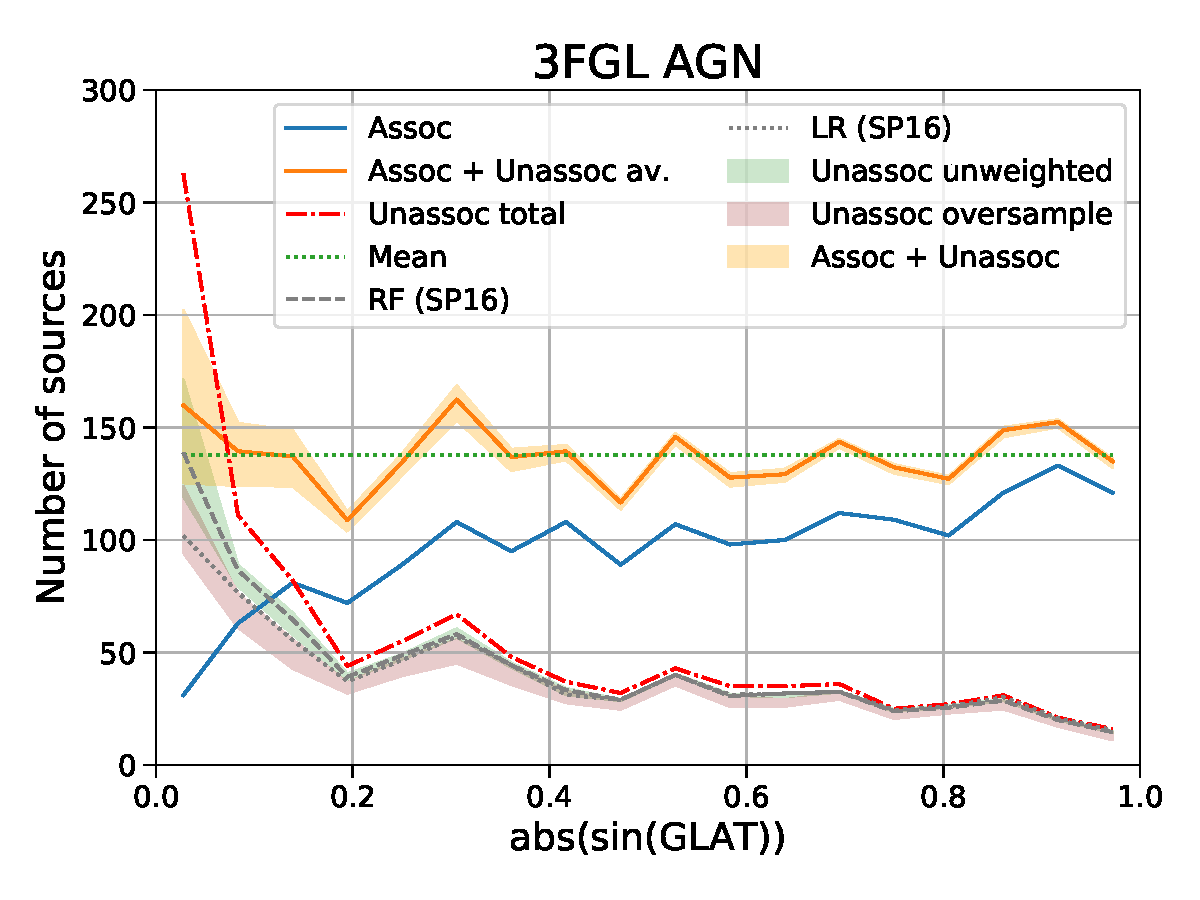
\includegraphics[width=0.45\textwidth]{plots/lat_profile_AGN_3FGL_oversample.pdf}
%\hspace*{-1cm}
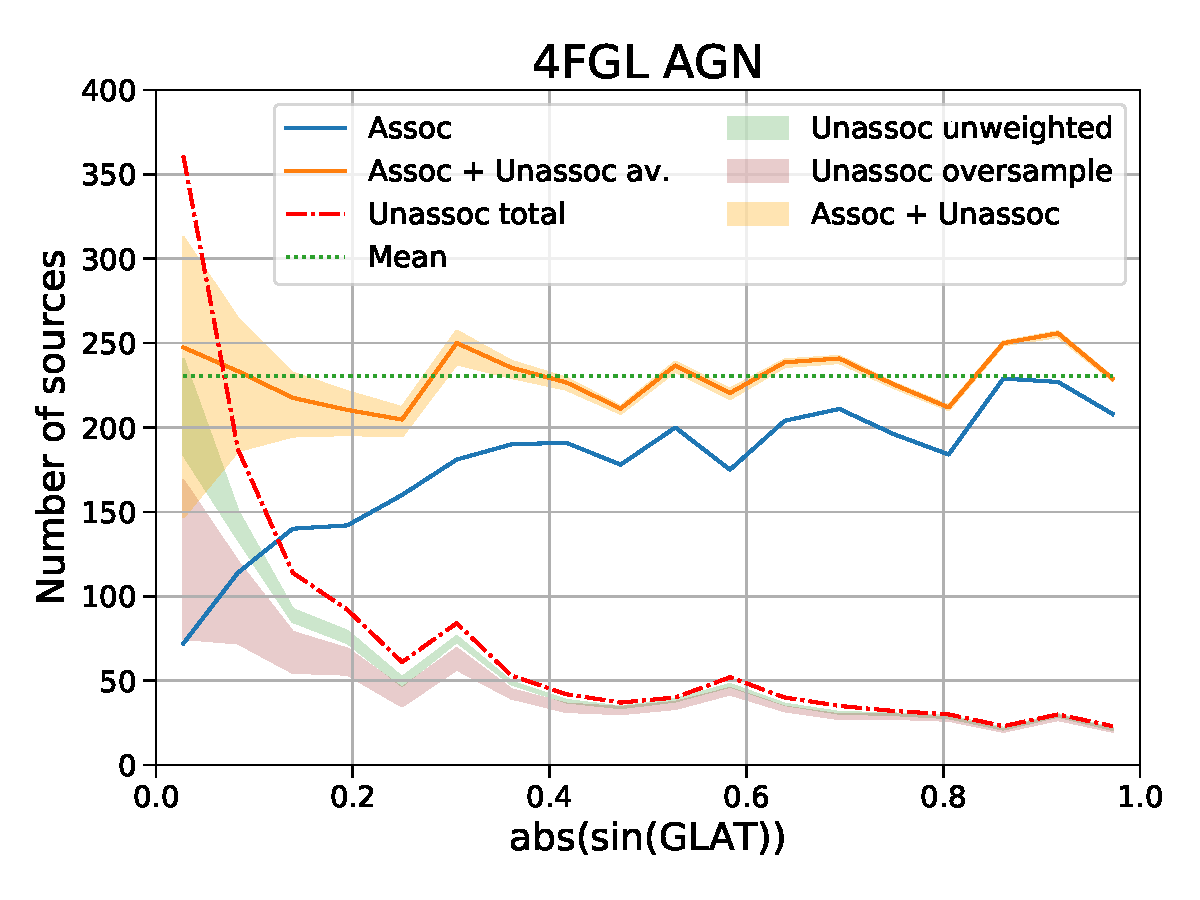
\includegraphics[width=0.45\textwidth]{plots/lat_profile_AGN_4FGL_oversample.pdf}
\caption{Latitude profiles of source counts. Blue solid line -- associated 3FGL and 4FGL sources. Red dash-dotted line -- all unassociated sources. Green (red) band -- envelope of sums of class probabilities for unassociated sources for the four ML algorithms without (with) oversampling. Orange solid line (band) -- average (envelope) of sums of class probabilities for the eight ML methods with and without oversampling added to the source count of associated sources. 
Green dashed line on the AGN plots -- mean of the sum of counts of associated sources and the average of the expectations for counts of unassociated sources (mean of the orange solid line).
Gray dashed (dotted) line -- RF (LR) sums of class probabilities from \cite{2016ApJ...820....8S}.
For details see Section \ref{sec:lat-lon-profiles}. }  
\label{fig:lat_profile}
\end{figure*}



\begin{figure*}[h]
\center
%\hspace*{-1cm}
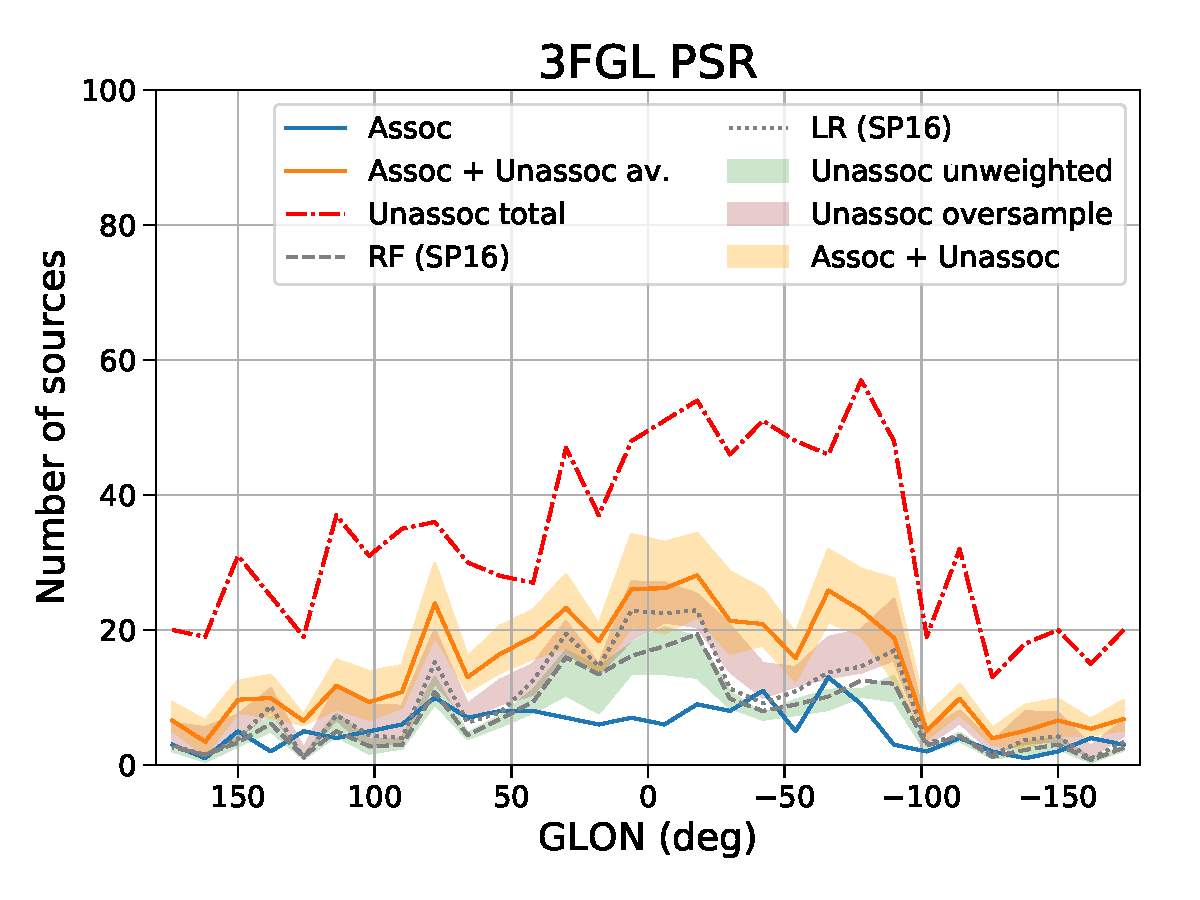
\includegraphics[width=0.45\textwidth]{plots/lon_profile_PSR_3FGL_oversample.pdf}
%\hspace*{-1cm}
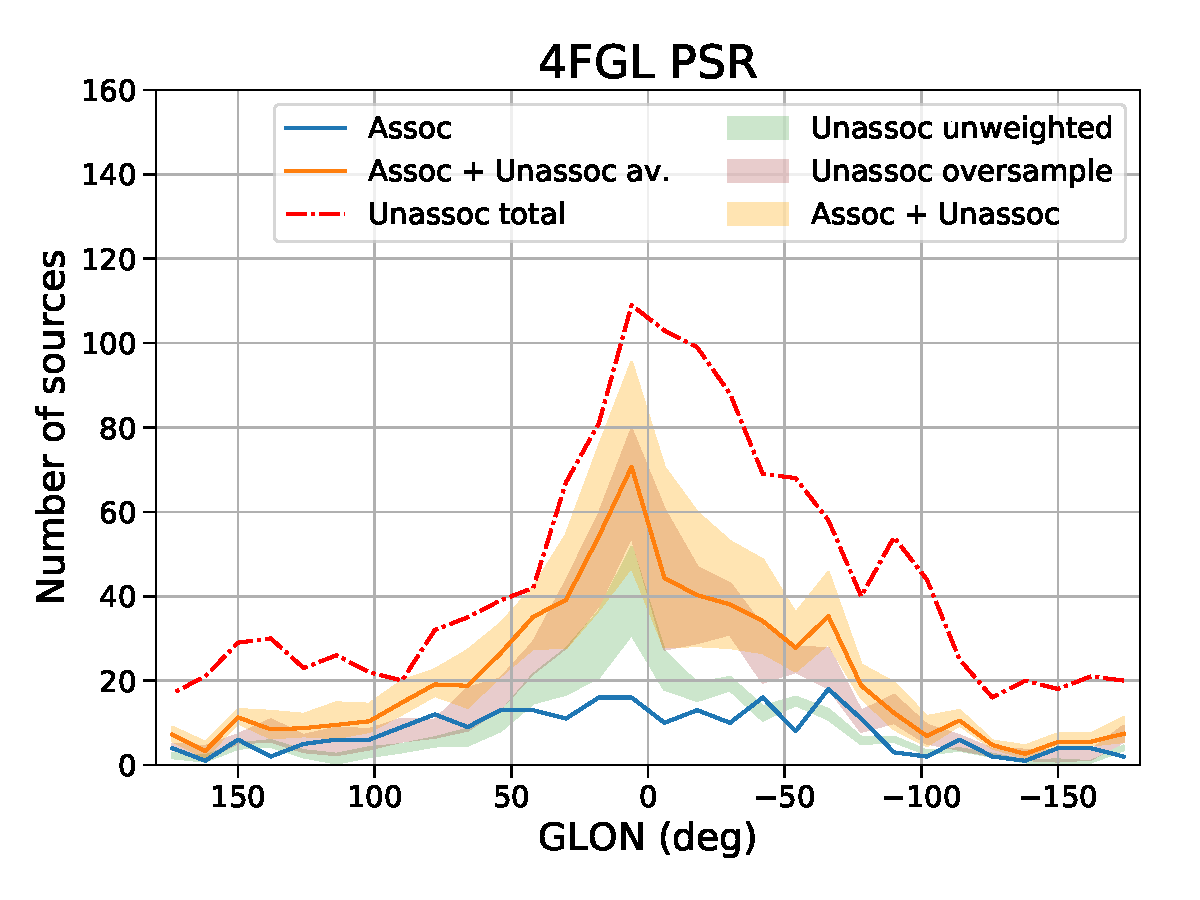
\includegraphics[width=0.45\textwidth]{plots/lon_profile_PSR_4FGL_oversample.pdf} \\
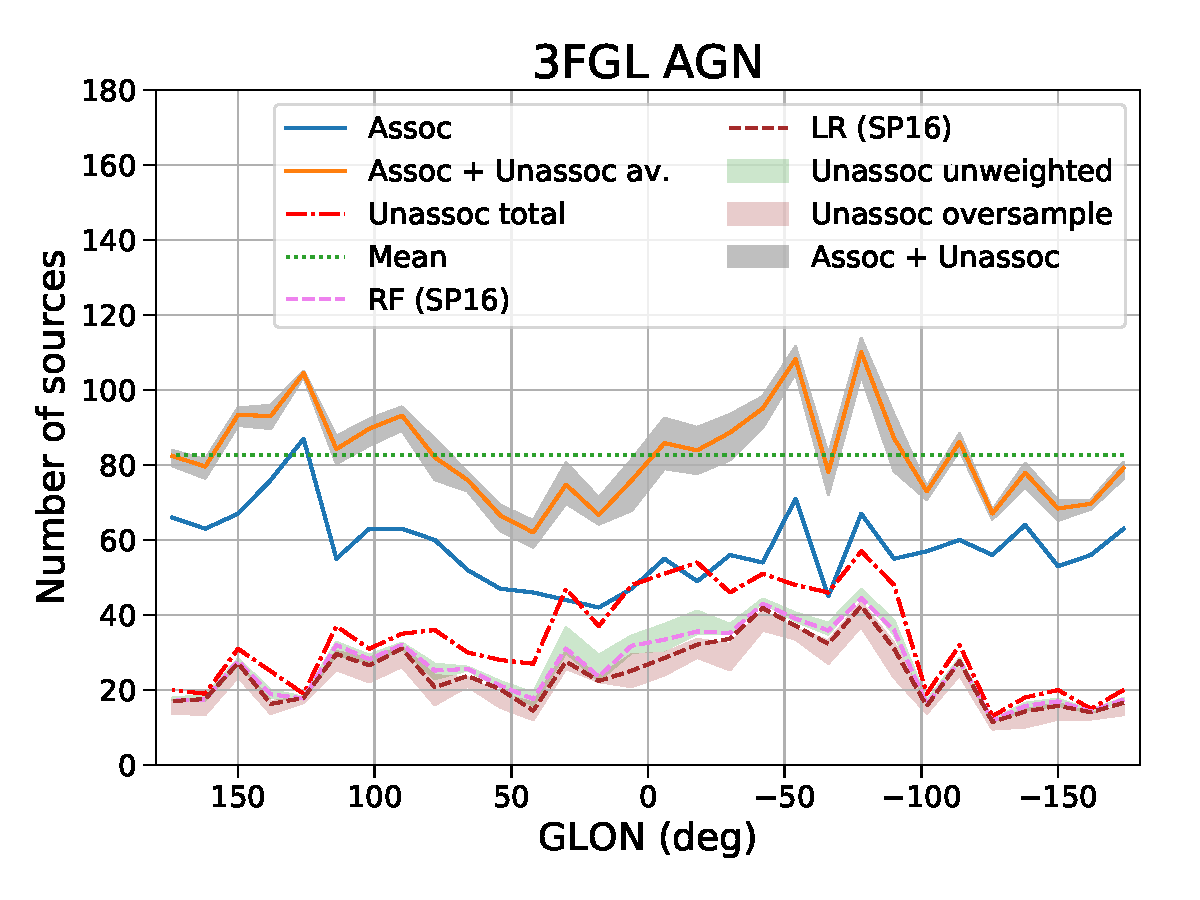
\includegraphics[width=0.45\textwidth]{plots/lon_profile_AGN_3FGL_oversample.pdf}
%\hspace*{-1cm}
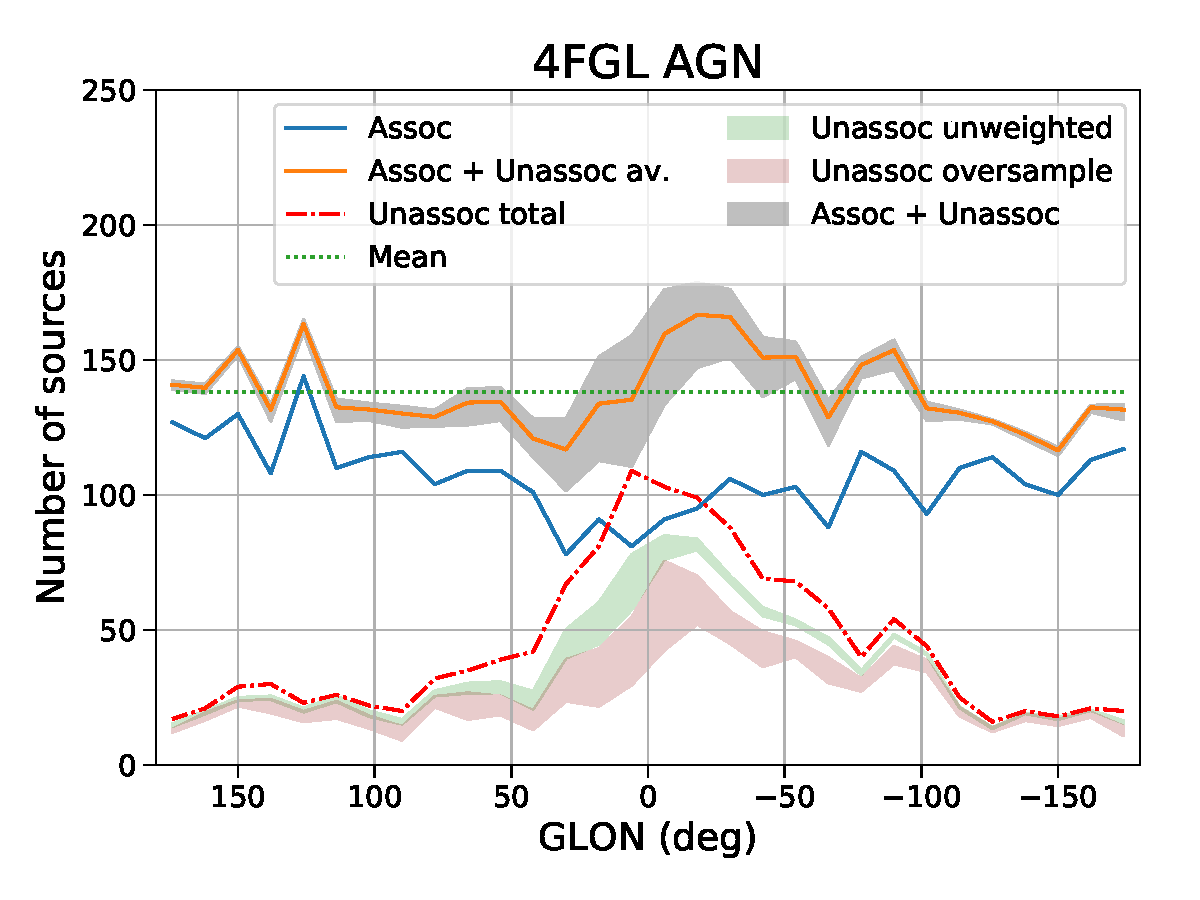
\includegraphics[width=0.45\textwidth]{plots/lon_profile_AGN_4FGL_oversample.pdf}
\caption{Longitude profiles of source counts. For the definition of labels see Figure \ref{fig:lat_profile}.}  
\label{fig:lon_profile}
\end{figure*}


In this section we show Galactic latitude and longitude profiles of the distributions of associated and unassociated sources.
In Figure \ref{fig:lat_profile} we present the source counts as a function of ${\rm abs(sin(GLAT))}$,
where we use 20 bins, i.e., each bin corresponds to a solid angle of $4 \pi / 20$. 
Solid blue lines show counts of associated sources in 3FGL and 4FGL catalogs.
It is interesting to note that the density of associated AGNs is decreasing near the Galactic plane.
The total counts of unassociated sources are shown by red dash-dotted lines.
Green shaded areas show the envelopes of sums of probabilities for AGN- and PSR-like sources for the four 
algorithms without oversampling, while the red shaded areas show the envelope for the four algorithms 
with oversampling.
The classifications of 3FGL sources by \cite{2016ApJ...820....8S} are shown by gray dashed (RF) and dotted (LR) lines.
In this section we do not perform a correction for the presence of other sources among the unassociated ones.
The numbers of unassociated sources classified as AGNs and PSRs grow towards the Galactic plane (GP).
Within $\approx 4^\circ\!\!.5$ from the GP the expected number of PSRs is about the same as the number of AGNs among unassociated sources (the first data point on the left).
At high latitudes, most of unassociated sources are classified as AGNs.
It is interesting to note, that according to Table \ref{tab:feat_imp}, GLAT is one of the least important features for the RF algorithm.
It can be a posteriori explained by the fact that
 the density of AGNs is such that even in the GP the expected number of AGNs is comparable to the expected number of PSRs.

Orange shaded areas show the sum of the source counts and the expected number of sources for the eight methods (both with and without oversampling).
The average among the eight methods added to the counts of associated sources is shown by solid orange line 
(for AGNs we also show the mean of these points by dotted green line).
We find that the number of associated AGNs is decreasing towards the GP, the expected number of AGNs among unassociated sources is increasing towards the GP, but the sum of the two is relatively uniform as a function of Galactic latitude.


In Figure \ref{fig:lon_profile} we show plots analogous to Figure \ref{fig:lat_profile} for Galactic longitudes.
We note that there is a significant increase in the number of unassociated sources in the 4FGL catalog for $|\ell | \lesssim 50^\circ$.
It leads to a large expected number of pulsars among unassociated sources for these longitudes.
The number of associated AGNs is smaller than average for $|\ell | \lesssim 50^\circ$, while the expected number of AGNs among unassociated sources is larger than average for these longitudes.
The sum of the two is relatively uniform, with a possible overprediction of AGNs in the unassociated sources in the 4FGL catalog for \mbox{$-50^\circ < \ell < 0^\circ$}.











\section{Conclusions}
\lb{sec:conclusions}

In the paper we determine the probabilities of classification of unassociated sources in the 3FGL and 4FGL \Fermi-LAT catalogs.
The probabilities are calculated with 4 different ML methods: random forests, boosted decision trees, logistic regression and neural networks.
The algorithms were trained and tested with associated sources.
We have also scanned some meta-parameters of the algorithms, such as depth of the trees, the number of trees, the number of neurons etc. in order to determine optimal parameters which do not create overfitting of data and provide good accuracy of classification.
The accuracy, which we obtained for the 3FGL catalog for all four algorithms, was about 97\%.
We have also checked the accuracy of classification by selecting unassociated sources in 3FGL, which have associations in 4FGL.
If we take the 4FGL associations as the true value, then the accuracy of classification in this subset of sources is between 93\% and 95\%.
As one can see from Figure \ref{fig:3FGL_vs_4FGL_classes}, the misclassified sources have spectral parameters in 3FGL which are typical of the other class, i.e., the misclassification can be due to problems with reconstructing the spectrum of the sources.

As a result of the analysis we create catalogs with probabilistic classifications of sources, where for each source and each class (i.e., AGNs and pulsars in our case) we report class probabilities for each of the four algorithms, i.e., 8 columns labeled by classes and by methods: ``AGN\_BDT'', ``PSR\_NN'' etc.
We report the classification probabilities not only for the unassociated sources, but also for the associated ones, which can be used to find outliers.
An advantage of such probabilistic classification is that a threshold on probability for selecting, e.g., pulsar candidates, can be chosen by the user based on his or her needs.
For example, in a search of new pulsars, one can select a low threshold in order to avoid missing possible pulsars.
In a derivation of an average property of the class, e.g., spectral index or cutoff energy, one can select a high threshold in order to avoid contamination from the other class, in addition one can use weighting by probability.
However, one should be careful here, since some of the properties of sources were used for the determination of probabilities,
the average of these features weighted by the probabilities can be biased compared to an average derived from multiwavelength associations.

As an example of the application of the probabilistic catalogs, we derive the expected number of sources in the catalog as a function of their flux, including the unassociated sources.
As a consistency check, we compare the counts of associated sources to the sums of probabilities for associated sources.
We find that correcting for the contribution of sources other than AGNs and pulsars plays an important role for estimation of the expected number of sources in a particular class.
We find the total expected number of AGNs and pulsars in 3FGL and 4FGL catalogs by adding the class probabilities in the unassociated sources to the source counts of associated sources and correcting for the contribution of other classes in the unassociated sources.
In particular, we find that the total expected number of pulsars is about two times larger than the number of associated pulsars.

We plot the counts of associated sources and the expected number of AGNs and pulsars among unassociated sources
as functions of Galactic latitude and longitude.
We find that the number of associated AGNs is decreasing towards low latitudes, while the expected number of AGNs among unassociated sources is increasing, but the sum of the two is relatively uniform, as expected for extragalactic sources.
We also find that the expected number of pulsars among unassociated 4FGL sources is significantly larger than average for longitudes 
$|\ell | \lesssim 50^\circ$.




\subsection*{Acknowledgements}

The authors would like to thank ...
for valuable comments and suggestions.
We would like to acknowledge the use of the following software:
Astropy \citep[\url{http://www.astropy.org},][]{2013A&A...558A..33A}, 
matplotlib \citep{Hunter:2007}, 
scikit-learn [\url{https://scikit-learn.org/stable/about.html}], 
TOPCAT \citep{2005ASPC..347...29T}.


\newpage
\bibliography{ML_3FGL_papers}  

\begin{appendix}
\section{Tests of additional meta-parameters}
\lb{sec:app}

In this appendix we discuss tests of some hyper-parameters, which had a relatively little effect on the 
accuracy of the algorithms. For these tests we use the 3FGL catalog.

LR algorithm has two hyper-parameters regularization and tolerance. 
%These features are the limit up to which one wants to go before accepting a solution. 
As can be seen in figure \ref{fig:LR_tol_reg} the effect on accuracy is less than 1\%. Therefore we used the default values for these parameters (tolerance is 1$e^{-4}$ and regularization parameter is set at 1).% \dima{If we mention the default value, we should say what the default values are}. 
\begin{figure}[h]
%\centerin
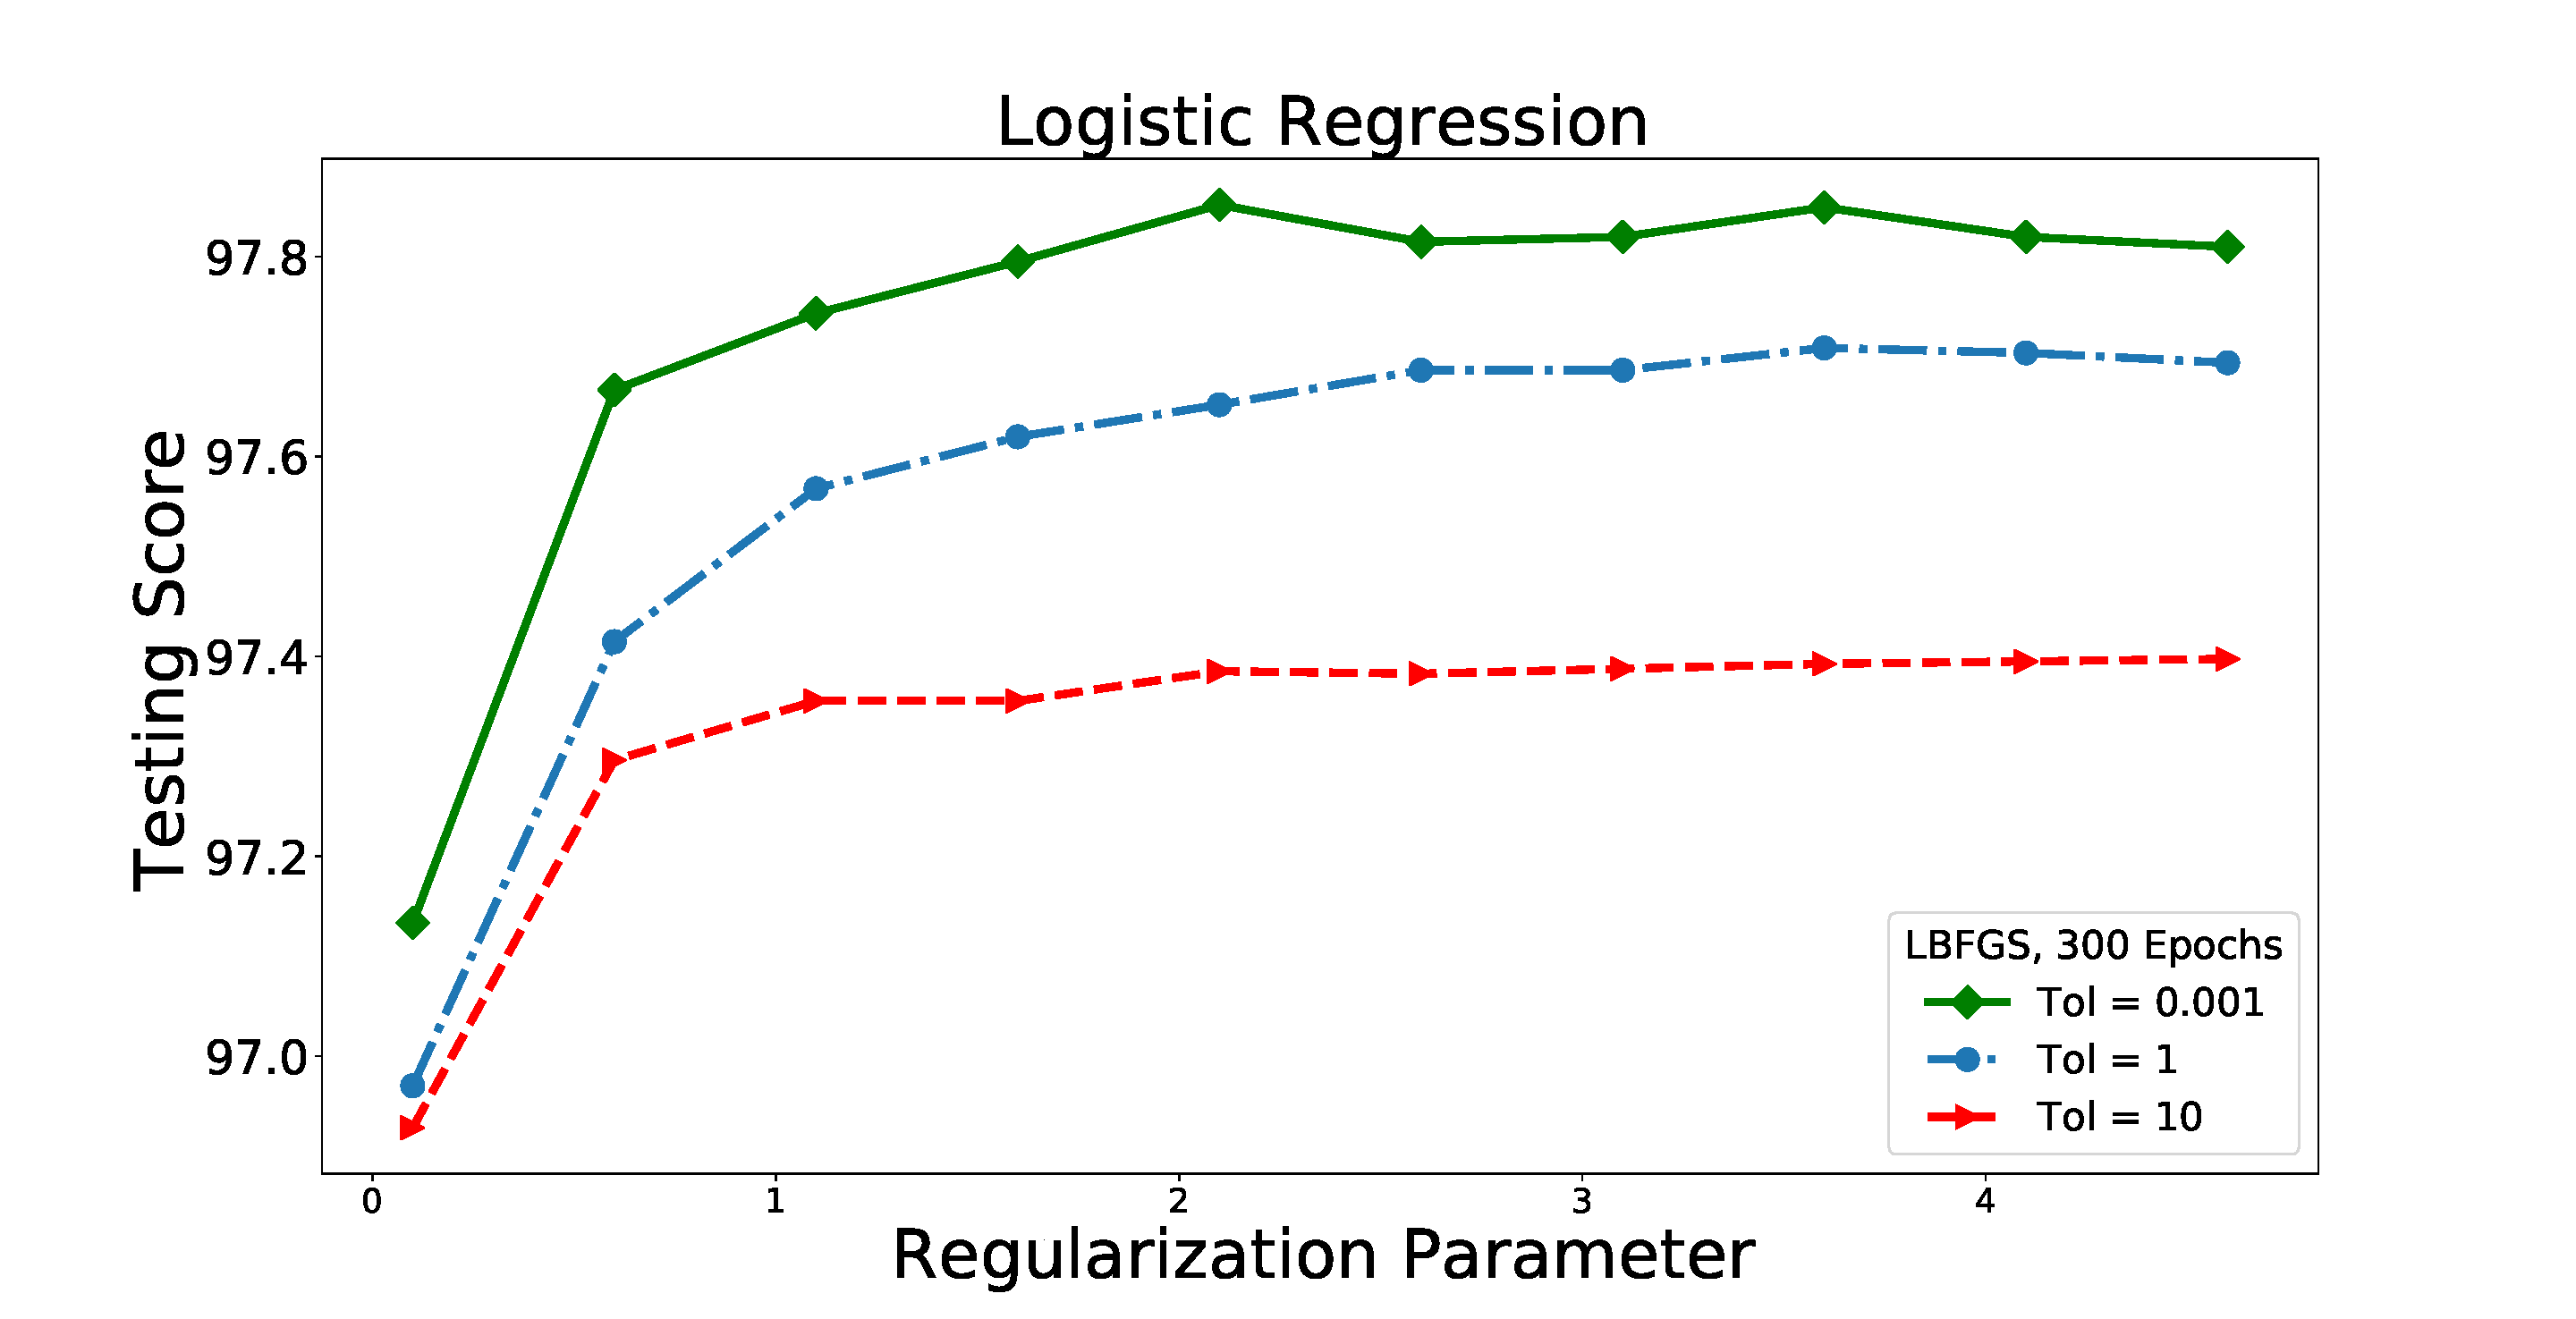
\includegraphics[width=\twopicsp\textwidth]{plots/lr_train_reg.pdf}
%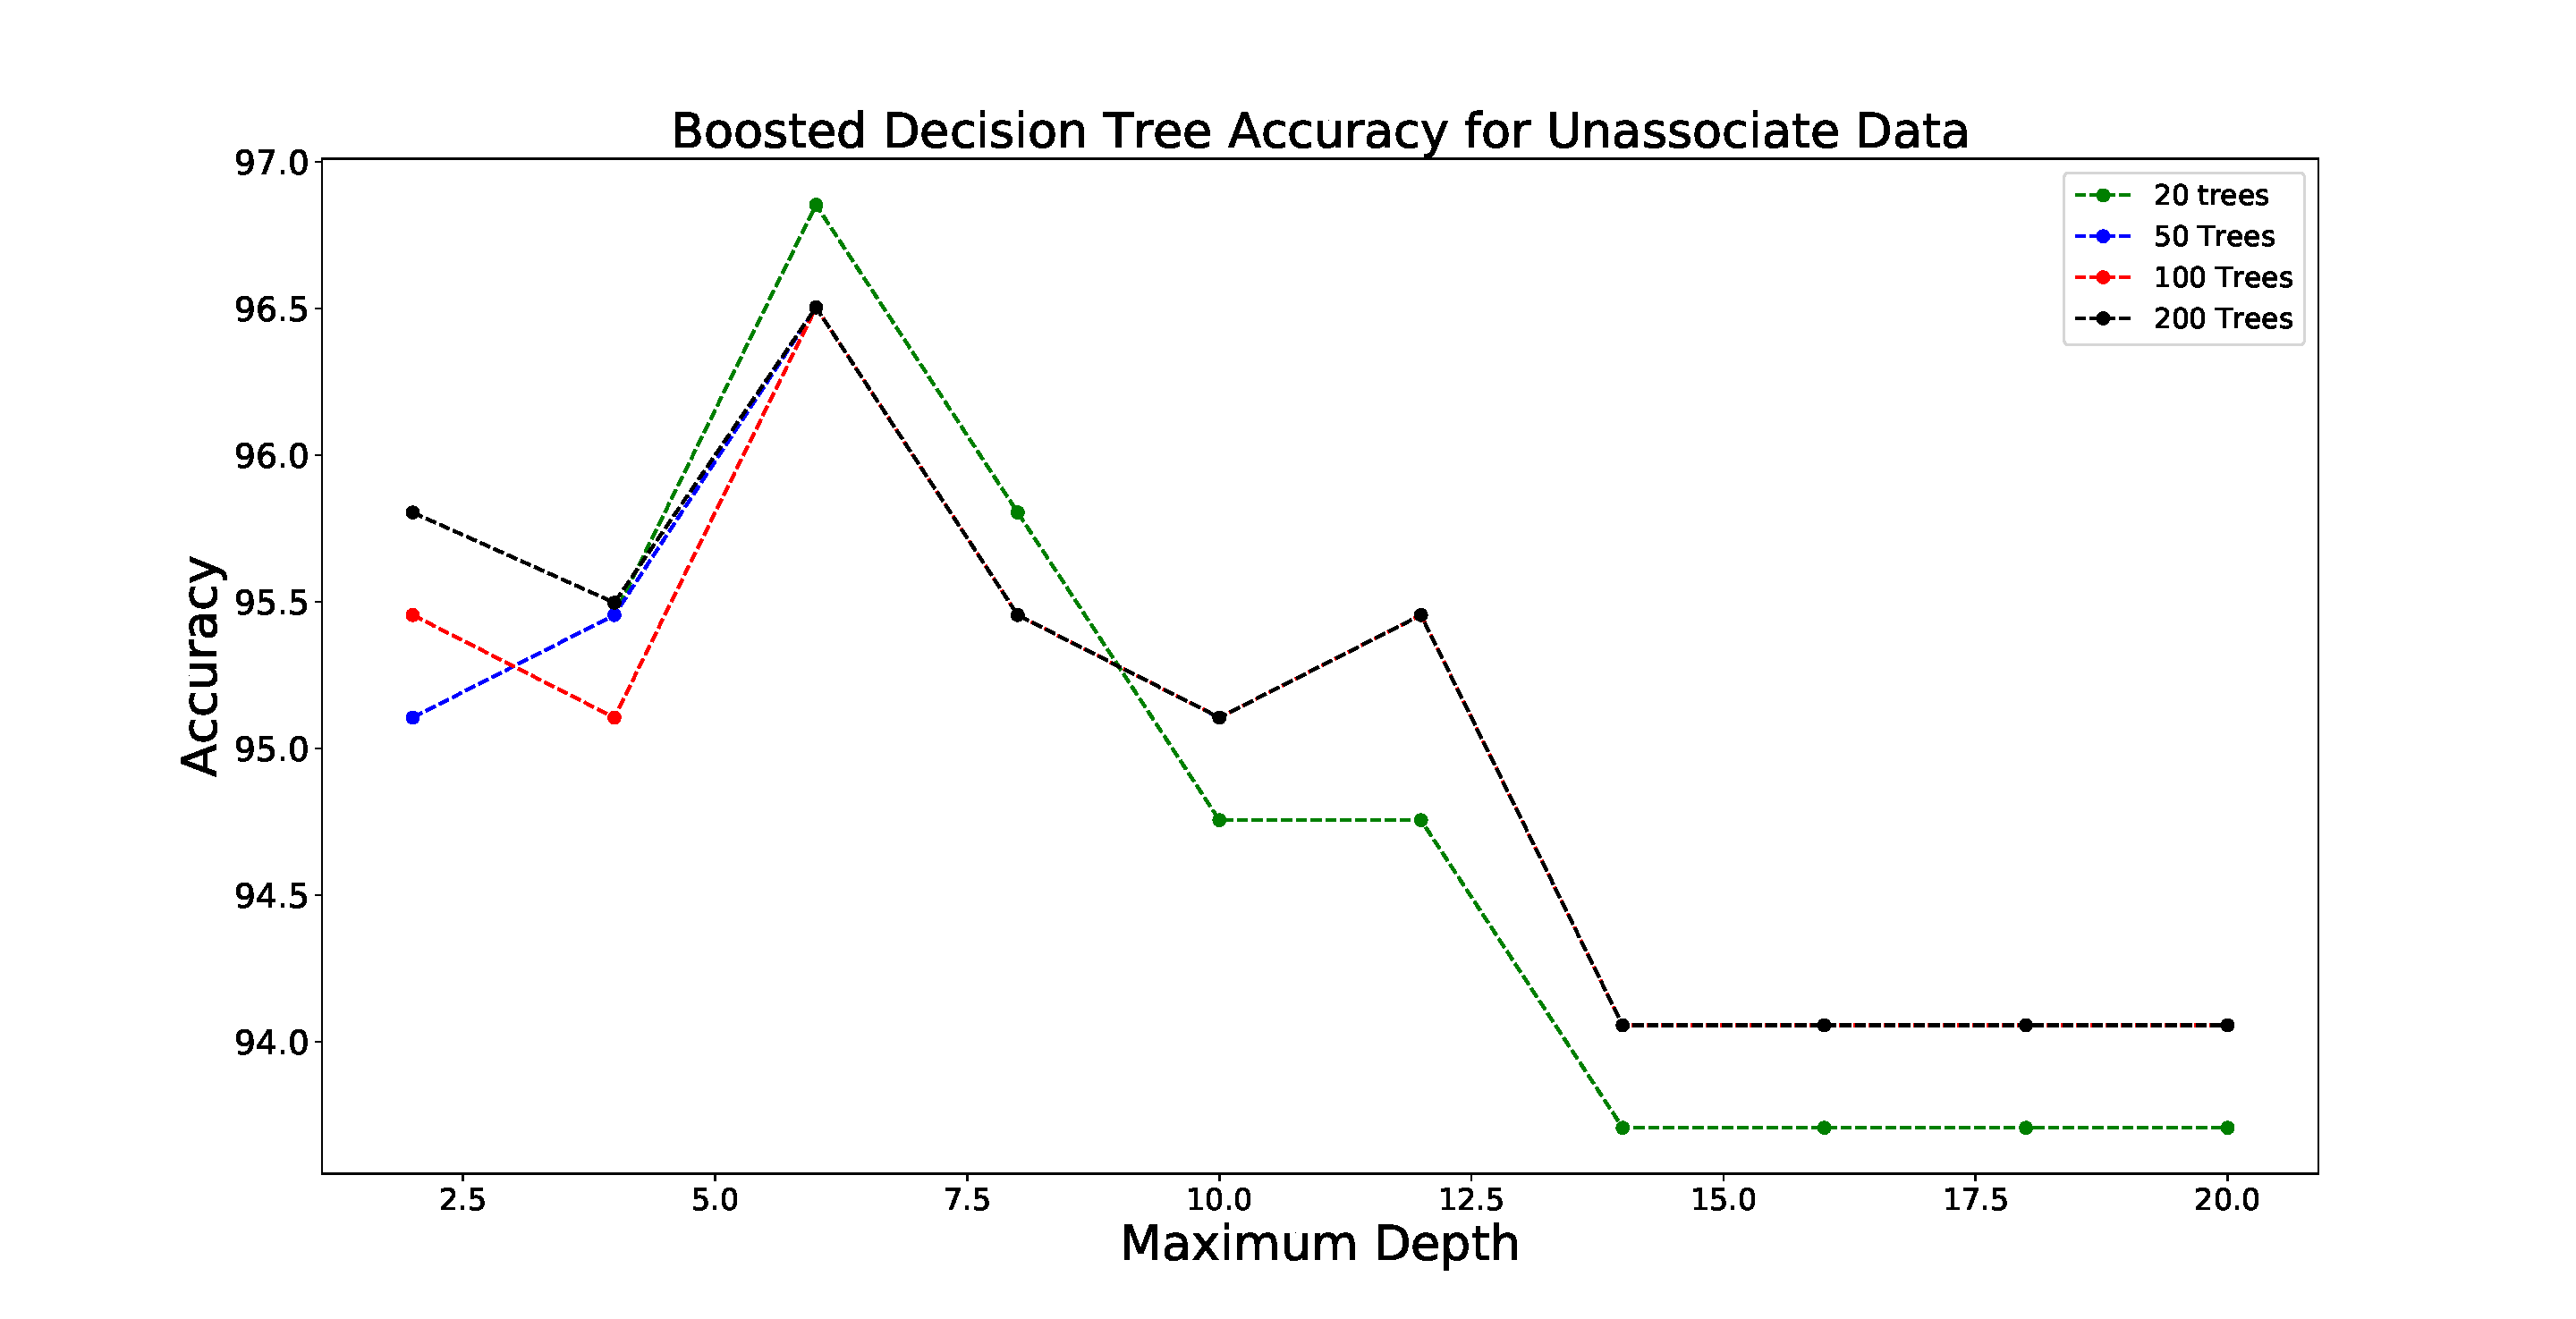
\includegraphics[width=\twopicsp\textwidth]{plots/unassoc_complex.pdf}
\caption{Dependence of LR on tolerance and regularization}
\label{fig:LR_tol_reg}
\end{figure}

In Figure \ref{fig:nn_nn} we show the effect of adding the second hidden layer in the NN algorithm.
The difference between the best accuracies with the additional hidden layer is less then 1\%
compared with the NN with one hidden layer (cf. Table \ref{tab:selected_algs}).
\begin{figure}[h]
%\centerin
\includegraphics[width=\twopicsp\textwidth]{plots/nn_2layers_3fgl.pdf}
%\includegraphics[width=\twopicsp\textwidth]{plots/unassoc_complex.pdf}
\caption{Dependence of NN on the second hidden layer, for 10 neurons in the first layer.}
%\dima{Strictly speaking this is the case of 3 hidden layers.}}
\label{fig:nn_nn}
\end{figure}

At the end we summarize features and their statistics,
which we use for probabilistic classification of sources in the 3FGL and 4FGL catalogs,
in Tables \ref{tab:3FGL_features} and \ref{tab:4FGL_features} respectively. 

\pgfplotstableread[col sep=comma]{tables/features/3fglassocfeaturesAGNPSRnewfeats.csv}\tablea
\begin{table}
\resizebox{0.45\textwidth}{!}{
\pgfplotstabletypeset[
columns={Name,Mean,SD,Minimum,Maximum},
column type=c,
string type,
every head row/.style={before row=\toprule,after row=\midrule,},
every last row/.append style={after row={\hline} },
every first column/.style={column type/.add={|}{}},
every last column/.style={column type/.add={}{|}},
columns/Name/.style={column name=Feature Name,string replace*={_}{\textunderscore}},
columns/Mean/.style={column name=Mean,column type=c,numeric type,fixed,precision=2},
columns/SD/.style={column name=Standard Deviation,numeric type,fixed,precision=2},
columns/Minimum/.style={column name=Minimum,numeric type,fixed,precision=2},
columns/Maximum/.style={column name=Maximum,numeric type,fixed,precision=2},
skip rows between index={11}{25}
]{\tablea}
}
\vspace{0.2cm}
\caption{Statistics of features used for 2 class probabilistic classification of the 3FGL sources.
\lb{tab:3FGL_features}}
\end{table}

\pgfplotstableread[col sep=comma]{tables/features/4fglassocfeatures.csv}\tableaf
\begin{table}
\resizebox{0.45\textwidth}{!}{
\pgfplotstabletypeset[
columns={Name,Mean,SD,Minimum,Maximum},
column type=c,
string type,
every head row/.style={before row=\toprule,after row=\midrule,},
every last row/.append style={after row={\hline} },
every first column/.style={column type/.add={|}{}},
every last column/.style={column type/.add={}{|}},
columns/Name/.style={column name=Feature Name,string replace*={_}{\textunderscore}},
columns/Mean/.style={column name=Mean,column type=c,numeric type,fixed,precision=2},
columns/SD/.style={column name=Standard Deviation,numeric type,fixed,precision=2},
columns/Minimum/.style={column name=Minimum,numeric type,fixed,precision=2},
columns/Maximum/.style={column name=Maximum,numeric type,fixed,precision=2},
%skip rows between index={17}{28}
]{\tableaf}
}
\vspace{0.2cm}
\caption{Statistics of features used for probabilistic classification of the 4FGL sources.
\lb{tab:4FGL_features}}
\end{table}




\end{appendix}

\end{document}

